\documentclass{article}
\usepackage{listings}
\usepackage{xcolor} % 
%in that file you will find the packages and other macro needed like \R for the real number set. 
\lstdefinestyle{Python-editor}{
    language=Python,
    numbers=left,
    frame=single,
    backgroundcolor=\color{gray!5},
    keywordstyle=\color{blue}\bfseries,
    stringstyle=\color{red},
    commentstyle=\color{green!50!black},
    basicstyle=\ttfamily\footnotesize,
    numberstyle=\tiny\color{gray},
    breaklines=true,
    captionpos=b
}
\input{Preamble}

\date{\today}

\begin{document}

%this creates the title page. You must complete the information there
\hypersetup{pageanchor=false} 
\begin{titlepage}
\newcommand{\HRule}{\rule{\linewidth}{0.5mm}} % Defines a new command for the horizontal lines, change thickness here

\center % Center everything on the page
 
%----------------------------------------------------------------------------------------
%   HEADING SECTIONS
%----------------------------------------------------------------------------------------

\vspace{3cm}
\textsc{\LARGE MATH-512 - Optimization on Manifolds}\\[1.5cm] % Name of your university/college
\textsc{\Large March 2025}\\[0.5cm] % Major heading such as course name
\textsc{\large }\\[0.5cm] % Minor heading such as course title

%----------------------------------------------------------------------------------------
%   TITLE SECTION
%----------------------------------------------------------------------------------------

\HRule \\[0.4cm] % line above and under the title
{ \huge \bfseries Project 1}\\[0.4cm] % Title of your document
\HRule \\[1.5cm]
 
%----------------------------------------------------------------------------------------
%   AUTHOR SECTION
%----------------------------------------------------------------------------------------

\Large{\textsc{Basseras} Théo} \\
\Large{\textsc{Coelho Lopes} Marta} \\
\Large{\textsc{Okamoto} Ryosei} \\ [6cm]

%----------------------------------------------------------------------------------------
%   LOGO SECTION
%----------------------------------------------------------------------------------------


\includegraphics[width=0.4\linewidth]{Logo}\\[1cm] % Include a department/university logo - this will require the graphicx package
 
%----------------------------------------------------------------------------------------

\vfill % Fill the rest of the page with whitespace

\end{titlepage}


\clearpage
\thispagestyle{empty}
\tableofcontents

\clearpage
\hypersetup{pageanchor=true} % to start numbering after title and ToC pages
\pagenumbering{arabic}
\setcounter{page}{1}





%\section*{Question 3}
%\[
%m(x, y) = \frac{1}{n} \sum_{i \in [n]} x_i^T y_i.
%\]

%Since \( m(x, y) \) is a polynomial in a finite-dimensional space, it is continuous. Therefore, we can take \( m \) as the Riemannian metric of \( OB(d, n) \) and we have m(x,v)=0 if x $\in OB(d,n)$ and v $\in$ $T_xOB(d,n)$.


\section*{The geometry of $\text{OB}(d, n)$}
\addcontentsline{toc}{section}{\protect\numberline{}The geometry of $\text{OB}(d, n)$}

\subsection*{Question 1}
$\mathcal{S}^{d-1} = f^{-1}(0)$, where $f: \mathbb{R}^d \to \mathbb{R}$ is defined by:
\[
    f(x) = 1 - x^T x.
\]
Moreover we have (since x $\neq0, ||x||=1$),
\[
\dim (\ker (df(x)) = dim (x^\perp)= d - 1 \quad \text{so} \quad \operatorname{rank} (df) = d - (d - 1) = 1.
\]
%\[
%\text{Hence, } \operatorname{rank} (f) = d - 1, \text{ so } f \text{ is full rank (since dim $S^{d-1}=d-1)$ .}
%\]
Since $f$ is smooth (being polynomial) and $df$ is full rank, it follows that $\mathcal{S}^{d-1}$ is a smooth embedded submanifold of $\mathbb{R}^d$. Hence, the manifold $\operatorname{OB}(d,n)$ is a smooth embedded submanifold of $\mathbb{R}^{d\times n}$ as it is a finite product of smooth manifolds.

Let's define the function $h: \mathbb{R}^{d \times n} \to \mathbb{R}$ as:
\[
    h(X) = \prod_{i \neq j} ||x_i - x_j||^2,
\]
where $h^{-1}(\{0\}) = \Delta$. Since $\{0\}$ is closed and $h$ is continuous (as it is the product of continuous functions), it follows that $\Delta$ is closed. Thus, $\operatorname{OB}(d,n) \setminus \Delta$= $\operatorname{OB}(d,n)$ $\cap$ $O$ ($O :=$ $\mathbb{R}^{d\times n} \setminus \Delta$ is an open in $\mathbb{R}^{d\times n}$)  is open in the manifold $\operatorname{OB}(d,n)$ by the subspace topology.
    
According to the course, an open subset of a manifold is itself a smooth embedded submanifold of the higher space, implying that $\mathcal{M}$ is a smooth submanifold of $\mathbb{R}^{d\times n}$. %Furthermore, since $h$ is smooth (being a polynomial in a finite-dimensional space), it follows that $\mathcal{M} \setminus \Delta$ is a smooth manifold.

\subsection*{Question 2}
Since $\text{OB}(d, n)$ is the product of $n$ spheres, its tangent space is the product of the tangent spaces of the spheres. We have that \( T_X \text{OB}(d, n) = r^{-1}(0) \), where \( r: \mathbb{R}^{d \times n} \to \mathbb{R} \) is defined (with \( f \) defined in Question 1) as:
\[
r(X) = \left( f(x_1), \dots, f(x_n) \right).
\]
Here, \( x_i \in \mathbb{R}^d \), and the differential of \( f \), denoted \( df(x_i)[h] \), is given by:
\[
df(x_i)[h] = -2 x_i^T h.
\]
Thus, we have:
\[
\ker \left( dr(X) \right) = \left\{ Z \in \mathbb{R}^{d \times n} \mid z_i \in x_i^\perp \text{ for every } i \in [1, n] \right\}.
\]
According to the course, \( T_X \text{OB}(d, n) = \ker \left( dr(x) \right) \).




We can define the projection \( p \) as follows:
\[
p(Z) = \left( z_1 - (x_1^T z_1) x_1, \dots, z_n - (x_n^T z_n) x_n \right).
\]
To verify that \( p \) is a projection, we check that applying \( p \) twice yields the same result:

\[
p(p(Z)) = p \left( z_1 - (x_1^T z_1) x_1, \dots, z_n - (x_n^T z_n) x_n \right).
\]

Applying \( p \) again,

\[
p(p(Z))_i = \left( z_i - (x_i^T z_i) x_i \right) - x_i^T \left( z_i - (x_i^T z_i) x_i \right) x_i.
\]

Expanding the inner term,

\[
x_i^T \left( z_i - (x_i^T z_i) x_i \right) = x_i^T z_i - (x_i^T z_i) (x_i^T x_i).
\]

Since \( x_i^T x_i = 1 \), we obtain:

\[
p(p(Z))_i = z_i - (x_i^T z_i) x_i - x_i \left( x_i^T z_i - (x_i^T z_i) \right) = z_i - (x_i^T z_i) x_i.
\]

Thus, \( p(p(Z)) = p(Z) \), confirming that \( p \) is a projection.

Next, we prove that \( \operatorname{Im}(p) = T_X \text{OB}(d, n) \) by double inclusion.

- Suppose \( Z \in T_X OB(d, n) \), meaning \( x_i^T z_i = 0 \) $\text{ }\forall i$. Then:
  \[
  z_i = z_i - 0 = z_i - (x_i^T z_i) x_i.
  \]
  Hence, \( Z = p(Z) \), so \( Z \in \operatorname{Im}(p) \).

- Suppose \( Z \in \operatorname{Im}(p) \), meaning \( Z = p(R) \) for some \( R \). Then:
  \[
  dr(X)(R)_i = -2 x_i^T \left( r_i - (x_i^T r_i) x_i \right).
  \]
  Expanding:
  \[
  -2 \left( x_i^T r_i - (x_i^T r_i) \|x_i\|^2 \right) = -2 (x_i^T r_i - x_i^T r_i).
  \]
  Since this simplifies to zero, we conclude that \( Z \in \ker(dr(X)) \), meaning \( Z \in T_X \text{OB}(d, n) \). 

Thus, we have shown \( \operatorname{Im}(p) = T_X \text{OB}(d, n) \).

Finally, let \( V \in T_X \text{OB}(d, n) \) and \( U \in \text{OB}(d, n) \). Then:
\[
(U - p(U))_i = x_i^T u_i x_i.
\]
Taking the inner product with \( v_i \):
\[
(U - p(U))_i^T v_i = x_i^T u_i x_i^T v_i=0 \text{ since we have \( x_i^T v_i = 0 \) because \( V \in T_X \text{OB}(d, n) \)}.
\]
Since \( V \in \ker(dr(X)) = T_X \text{OB}(d, n) \), this leads to:
\[
\langle U-p(U),V\rangle=\sum_{i \in [n]} (U - p(U))_i^T v_i = 0
\]
where the inner product is defined in the next question. Thus, \( p \) is the orthogonal projector onto \( T_X \text{OB}(d, n) \).

\subsection*{Question 3}
Let $\langle u, v \rangle_x = u^Tv$ be the inner product on the sphere $\mathcal{S}^{d-1}$, for $x\in\mathcal{S}^{d-1}$ and $u, v\in T_x\mathcal{S}^{d-1}$. We then define an inner product on $\text{OB}(d, n)$, the product of $n$ spheres, as $\langle U, V\rangle_X = \sum_{i=1}^n\langle u_i, v_i\rangle_{x_i} = \sum_{i=1}^n u_i^Tv_i$, where $U=[u_1\ldots u_n], V=[v_1\ldots v_n]$ and $X=[x_1\ldots x_n]$. We claim that
$$
\begin{array}{ccccc}
\langle\cdot, \cdot\rangle_X & : & T_X\text{OB}(d, n) \times T_X\text{OB}(d, n) & \to & \mathbb{R} \\
 & & (U, V) & \mapsto & \langle U, V\rangle_X = \sum_{i=1}^n u_i^Tv_i = \text{tr}(U^TV)\\
\end{array}
$$
is a Riemannian metric on $\text{OB}(d, n)$. We verify that it satisfies bilinearity, symmetry, positive definiteness and that it varies smoothly with $X$.
\begin{itemize}
    \item Bilinearity: Let $\lambda \in \mathbb{R}$ and $U, V, U_1, U_2, V_1, V_2\in T_X\text{OB}(d, n)$. Then
    \begin{align*}
        & \langle \lambda U, V\rangle_X = \sum_{i=1}^n\lambda u_i^Tv_i = \lambda\sum_{i=1}^nu_i^Tv_i = \lambda\langle U, V\rangle_X\\
        & \langle U, \lambda V\rangle_X = \sum_{i=1}^n u_i^T\lambda v_i = \lambda\sum_{i=1}^nu_i^Tv_i = \lambda\langle U, V\rangle_X\\
        & \langle U_1 + U_2, V\rangle_X = \sum_{i=1}^n(u_{1_i}+u_{2_i})^Tv_i = \sum_{i=1}^nu_{1_i}^Tv_i + \sum_{i=1}^nu_{2_i}^Tv_i = \langle U_1, V\rangle_X + \langle U_2, V\rangle_X\\
        & \langle U, V_1 + V_2\rangle_X = \sum_{i=1}^nu_i^T(v_{1_i}+v_{2_i}) = \sum_{i=1}^nu_i^Tv_{1_i} + \sum_{i=1}^nu_i^Tv_{2_i} = \langle U, V_1\rangle_X + \langle U, V_2\rangle_X.
    \end{align*}
    \item Symmetry: Let $U, V\in T_X\text{OB}(d, n)$. Then
    $$
    \langle U, V\rangle_X = \sum_{i=1}^n u_i^Tv_i = \sum_{i=1}^nv_i^Tu_i = \langle V, U\rangle_X.
    $$
    \item Positive definiteness: Let $U\in T_X\text{OB}(d, n)$. Then
    $$
    \langle U, U\rangle_X = \sum_{i=1}^nu_i^Tu_i = \sum_{i=1}^n\|u_i\|^2 \geq 0.
    $$
    Moreover, $\langle U, U\rangle_X = 0 \iff \|u_i\|=0\text{ }\forall i\in\{1, \ldots, n\}$, i.e. $\langle U, U\rangle_X = 0 \iff U=0$.
    \item Riemannian metric: Let $V(x), W(x)$ be two smooth vector fields on $\text{OB}(d, n)$. Then, $\langle V(X), W(X)\rangle_X = \sum_{i=1}^nv_i(X)^Tw_i(X)$. Each term in the sum is a product of smooth functions by assumption and is thus also smooth. The sum is then a sum of smooth functions and is thus also smooth. This proves that the metric $\langle\cdot, \cdot\rangle_X$ is a Riemannian metric.
\end{itemize}
Notice that the chosen Riemannian metric is the restriction of the inner product of the Euclidean space $\mathbb{R}^{d\times n}$ to the tangent spaces. As such, $\text{OB}(d, n)$ with this Riemannian metric inherited from $\mathbb{R}^{d\times n}$ is a Riemannian submanifold of $\mathbb{R}^{d\times n}$. This is going to be particularly useful when computing Riemannian gradients of functions defined over $\text{OB}(d, n)$.

\subsection*{Question 4}
Let's take $R:T\text{OB}(d, n)\rightarrow \text{OB}(d, n)$, which is clearly smooth:
\[
R_X(V)= \left(\frac{x_1 + tv_1}{\|x_1 + tv_1\|}, \dots, \frac{x_n + tv_n}{\|x_n + tv_n\|} \right).
\]

Define the curve:
\[
c(t) = R_X(tV).
\]

At \( t = 0 \), we have:
\[
c(0) = R_X(0) = (x_1, \dots, x_n)=X.
\]

Now, differentiate \( c(t) \) component-wise:
\[
c'(t)_i = \frac{d}{dt} \left( \frac{x_i + tv_i}{\|x_i + tv_i\|} \right).
\]

Using the quotient rule, we compute:

\[
c'(t)_i = \frac{\|x_i + tv_i\| \cdot v_i - (x_i + tv_i) \cdot \frac{d}{dt} \|x_i + tv_i\|}{\|x_i + tv_i\|^2}.
\]

Since
\[
\frac{d}{dt} \|x_i + tv_i\| = \frac{(x_i + tv_i)^T v_i}{\|x_i + tv_i\|}
\]

at \( t = 0 \), we get:

\[
c'(0)_i = \frac{\|x_i\| v_i - x_i \cdot \frac{x_i^T v_i}{\|x_i\|}}{\|x_i\|^2}.
\]

Now, since \( x_i^T v_i = 0 \) ($V\in T_X\text{OB}(d, n)$), we simplify:

\[
c'(0)_i = \frac{\|x_i\| v_i}{\|x_i\|^2} = \frac{v_i}{\|x_i\|}=v_i.
\]

This confirms that:

\[
\left. \frac{d}{dt} R_X(tV) \right|_{t=0} = V.
\]

Thus, \( R_X(V) \) satisfies the first-order condition for a retraction.

Then, the second condition is clearly satisfied. Indeed, for each \( i \), we have:

\[
\frac{(x_i + tv_i)^T (x_i + tv_i)}{\|x_i + tv_i\|^2}.
\]

Expanding both the numerator and denominator:

\[
(x_i + tv_i)^T (x_i + tv_i) = \|x_i + tv_i\|^2.
\]

Thus, we get:

\[
\frac{\|x_i + tv_i\|^2}{\|x_i + tv_i\|^2} = 1.
\]

This confirms that for every $ i \in [n], R_X(V)_i \in \mathcal{S}^{d-1}$ so $R_X(V) \in OB(d,n)$.

Hence $R_V(X)$ is a retraction.

\subsection*{Question 5}
\subsubsection*{(a)}
The following code samples a point from $\text{OB}(d, n)$ uniformly at random.
\begin{lstlisting}[language=Python, numbers=left, frame=single, numbersep = 5pt, numberstyle=\tiny\color{gray}, backgroundcolor=\color{gray!5}, keywordstyle=\color{blue}, stringstyle=\color{red}, commentstyle=\color{green!50!black}, basicstyle=\ttfamily\small, showstringspaces=false, tabsize=4, breaklines=true]
import numpy as np 
import matplotlib.pyplot as plt

d = 5
n = 10

def sampleOB(d=5, n=10):
    L = [] # Vector that we sample in OB(d,n)
    for k in range(n):
        point = np.random.randn(d) # Generates a random vector in R^d
        if np.linalg.norm(point) != 0:
            L.append(point / np.linalg.norm(point)) # Put this vector on the Sphere and add it to the global vector L
        else: # Probability to have 0 a point on a continuous space is 0
            return sampleOB(d, n)
    return L
\end{lstlisting}

\subsubsection*{(b)}
The following code computes the orthogonal projection.
\begin{lstlisting}[language=Python, numbers=left, frame=single, numbersep = 5pt, numberstyle=\tiny\color{gray}, backgroundcolor=\color{gray!5}, keywordstyle=\color{blue}, stringstyle=\color{red}, commentstyle=\color{green!50!black}, basicstyle=\ttfamily\small, showstringspaces=false, tabsize=4, breaklines=true]
def orthogonal(x, L):
    O = []
    for i in range(len(L)):
        O.append(L[i] - x[i].T.dot(L[i]))  # Compute the orthogonal
    return O
\end{lstlisting}

\subsubsection*{(c)}
The following code computes the value of the metric.
\begin{lstlisting}[language=Python, numbers=left, frame=single, numbersep = 5pt, numberstyle=\tiny\color{gray}, backgroundcolor=\color{gray!5}, keywordstyle=\color{blue}, stringstyle=\color{red}, commentstyle=\color{green!50!black}, basicstyle=\ttfamily\small, showstringspaces=false, tabsize=4, breaklines=true]
def metric(U, V):
    m = 0
    for k in range(len(U)):
        m += U[k].T.dot(V[k]) # Compute the metric
    m = m / len(U)
    return m
\end{lstlisting}

\subsubsection*{(d)}
The following code samples a random tangent vector of unit norm.
\begin{lstlisting}[language=Python, numbers=left, frame=single, numbersep = 5pt, numberstyle=\tiny\color{gray}, backgroundcolor=\color{gray!5}, keywordstyle=\color{blue}, stringstyle=\color{red}, commentstyle=\color{green!50!black}, basicstyle=\ttfamily\small, showstringspaces=false, tabsize=4, breaklines=true]
def sample_tangent_vector(x):
    Vector=np.random.normal(0, 1e10,np.shape(x))*sampleOB() #sample a random vector (the norm of the vector does not really matter)
    tangent_vector=orthogonal(x,Vector) #projects the random vector on the 
    norm=np.linalg.norm(tangent_vector)
    if norm!=0:
        return(tangent_vector/norm)
    return(sample_tangent_vector(x))
\end{lstlisting}


\subsubsection*{(e)}
The following code computes the retraction.
\begin{lstlisting}[language=Python, numbers=left, frame=single, numbersep = 5pt, numberstyle=\tiny\color{gray}, backgroundcolor=\color{gray!5}, keywordstyle=\color{blue}, stringstyle=\color{red}, commentstyle=\color{green!50!black}, basicstyle=\ttfamily\small, showstringspaces=false, tabsize=4, breaklines=true]
def retraction(x, v):
    R = [] # The value of the retraction
    for i in range(len(x)):
        R.append((x[i] + v[i]) / np.linalg.norm(x[i] + v[i])) # For every coordinate we compute the retraction
    return R
\end{lstlisting}

\subsection*{Question 6}
Here is the code that verifies the projection property:

\begin{lstlisting}[language=Python, numbers=left, frame=single, numbersep = 5pt, numberstyle=\tiny\color{gray}, backgroundcolor=\color{gray!5}, keywordstyle=\color{blue}, stringstyle=\color{red}, commentstyle=\color{green!50!black}, basicstyle=\ttfamily\small, showstringspaces=false, tabsize=4, breaklines=true]
def projection_test():
    x=sampleOB()
    v=sampleOB()
    if not np.isclose(np.array(orthogonal(x,orthogonal(x,v))),np.array(orthogonal(x,v)),1e-10).all():
        print("projector property not verified")
    if not (np.isclose(np.array(orthogonal(x,x)),np.array([[[0]*d]*n]),1e-10).all()):
        print("projector does not project on the right space")
        print(orthogonal(x,x))
        return
    print("projection is perfect, well done")
    return
\end{lstlisting}


For the metric, we verify that it is positive definite, symmetric, and bilinear.

\begin{lstlisting}[language=Python, numbers=left, frame=single, numbersep = 5pt, numberstyle=\tiny\color{gray}, backgroundcolor=\color{gray!5}, keywordstyle=\color{blue}, stringstyle=\color{red}, commentstyle=\color{green!50!black}, basicstyle=\ttfamily\small, showstringspaces=false, tabsize=4, breaklines=true]
def Metric_test():
    v1=sampleOB()
    v2=sampleOB()
    v3=sampleOB()
    if not np.isclose(metric(v1,v2),metric(v2,v1),1e-10):
        print ("non symetric")
    if metric(v1,v1)<0:
        print("non positive")
    if metric(v1,v1)==0:
        if not np.isclose(sum(v1),0,1e-10):
            print('non definite')
    if not np.isclose(metric([3 * a + b for a, b in zip(v1, v2)],v3),3*metric(v1,v3)+metric(v2,v3),1e-10):
        print("not bilinear")
    print("Metric is perfect, well done")
    return
\end{lstlisting}


For the retraction, we check that its image is within the OB manifold \( \text{OB}(d, n) \).

\begin{lstlisting}[language=Python, numbers=left, frame=single, numbersep = 5pt, numberstyle=\tiny\color{gray}, backgroundcolor=\color{gray!5}, keywordstyle=\color{blue}, stringstyle=\color{red}, commentstyle=\color{green!50!black}, basicstyle=\ttfamily\small, showstringspaces=false, tabsize=4, breaklines=true]
def retraction_test():
    x=sampleOB()
    v=sample_tangent_vector(x)
    r=retraction(x,v)
    for i in range(len(x)):
        if np.isclose(r[i].T.dot(r[i]),1e-10):
            print("retraction is not in the sphere")
            print(i)
            return
    print("retraction is perfect, well done")
    return
\end{lstlisting}

\begin{figure}[H] 
  \centering  
  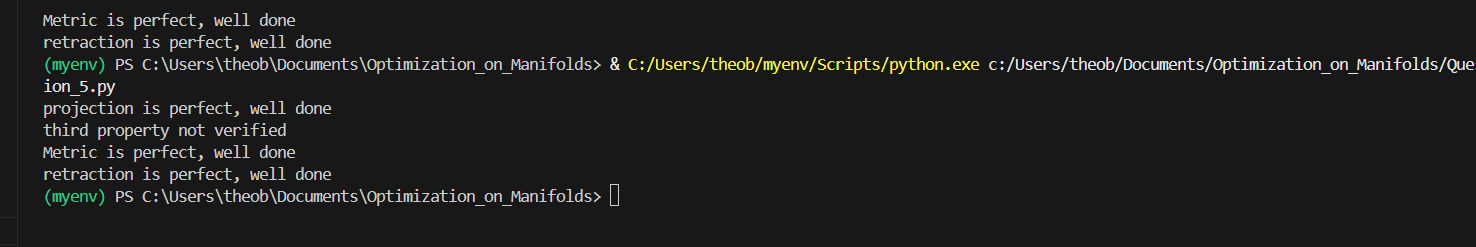
\includegraphics[width=0.5\textwidth]{Question6_compilation.png}  
  \caption{Compilation of the tests}  
  \label{fig:sample_image}  
\end{figure}

\newpage

\section*{Implementing RGD with a line-search}
\addcontentsline{toc}{section}{\protect\numberline{}Implementing RGD with a line-search}
\subsection*{Question 7}
We determine how many floating point operations are needed for computing $f$ at a given point $X$, where $f$ is defined as
$$
f(x_1, \ldots, x_n) = -\frac{2}{n(n-1)} \sum_{i<j} \log(1-x_i^Tx_j).
$$
Since $x_i$ and $x_j$ are vectors in $\mathbb{R}^d$, their inner product $x_i^Tx_j$ consists of $d$ multiplications and $d-1$ additions, which yields $2d-1$ operations. Performing then the subtraction $1-x_i^Tx_j$ and taking the logarithm $\log(1-x_i^Tx_j)$ give two more operations, leading to $2d+1$ operations. The sum over $i<j$, where $1\leq i < j \leq n$, is a sum over $\binom{n}{2}=n(n-1)/2$ elements. Thus, the $2d-1$ operations will be performed $n(n-1)/2$ times, which gives a total of
$$
(2d+1)\cdot \frac{n(n-1)}{2} = dn(n-1) + \frac{n(n-1)}{2} = dn^2 + \frac{n^2}{2} - dn -\frac{n}{2}.
$$
Finally, multiplying the sum by the constant $-2/(n(n-1))$ counts as one operation and does not change the leading term of the above expression, which is given by $dn^2$. Hence, the evaluation of $f$ at $X$ requires approximately $n^2d$ floating point operations.
% maybe for this question 8, show f is smooth locally at all x because there is an open set containing x and a smooth extension fbar such that f is equal to fbar restricted to x
\subsection*{Question 8}
We showed in question $3$ that $\mathcal{M}$ is a Riemannian submanifold of $\mathbb{R}^{d\times n}$ which inherits its inner product. Moreover, we notice that $f$ is a smooth function on $\mathcal{M}$, as it is a sum of compositions of smooth functions. Indeed, since $x_i\in\mathbb{S}^{d-1} \text{ }\forall i$, $x_i^Tx_j = \|x_i\|\|x_j\|\cos\angle(x_i, x_j) = \cos\angle(x_i, x_j)\leq 1$ and recall that we have removed the set of matrices for which $x_i^Tx_j=1$; thus, the logarithm $\log(1-x_i^Tx_j)$ is well-defined. Alternatively, we can directly show that $\forall X \in \mathcal{M}$, there exists an open neighborhood $U_X$ of $X$ and a smooth extension $\Bar{f}:U_X\rightarrow \mathbb{R}$ of $f$ such that $f = \Bar{f}|_{\mathcal{M}}$. We claim that we can take $U_X=\{X\in\mathbb{R}^{d\times n}: x_i^Tx_j < 1 \text{ } \forall i\neq j\}$ and $\Bar{f}:U_X\rightarrow \mathbb{R}$ defined by the same expression as $f$. First, since $\Bar{f}$ is well-defined on $U_X$, where the logarithm exists, and since it is infinitely continuously differentiable in the Euclidean sense, it is smooth. Moreover, by the arguments above, $U_X$ clearly contains $X$, as $X\in\text{OB}(d, n)\backslash\Delta$ and thus indeed satisfies $x_i^Tx_j < 1 \text{ }\forall i\neq j$. It thus remains to show that $U_X$ is open in $\mathbb{R}^{d\times n}$. To this end, define functions $g_{ij}:\mathbb{R}^{d\times n}\rightarrow\mathbb{R}, X\mapsto x_i^Tx_j$, which are clearly continuous. Upon noticing that $U_X = \cap_{i\neq j} g_{ij}^{-1}((-\infty, 1))$ and that $(-\infty, 1)$ is open in $\mathbb{R}$, we get that $U_X$ is itself open in $\mathbb{R}^{d\times n}$ by continuity of $g_{ij}$, as it is an intersection of open sets. Therefore, one can compute the Riemannian gradient of $f$ by computing the Euclidean gradient of $\Bar{f}$ and then projecting it orthogonally onto the tangent space of $X$:
$$
\text{grad}f(X) = \text{Proj}_X(\text{grad}\Bar{f}(X)),
$$
where $\text{Proj}_X: \mathbb{R}^{d\times n}\rightarrow T_X\text{OB}(d, n)$ was defined in question 2.\\
Before computing the Euclidean gradient of $\Bar{f}$, we rewrite $f$ equivalently as follows:
\begin{align*}
    f(x_1, \ldots, x_n) &= -\frac{2}{n(n-1)}\cdot \frac{1}{2}\sum_{i=1}^n\sum_{\substack{j=1\\j\neq i}}^n\log(1-x_i^Tx_j)\\
    &= -\frac{1}{n(n-1)}\sum_{i=1}^n\sum_{\substack{j=1\\j\neq i}}^n\log(1-x_i^Tx_j).
\end{align*}
We compute now the partial derivative of this last expression with respect to $x_i$ to obtain
\begin{align*}
    (\text{grad}\Bar{f}(X))_i &= -\frac{1}{n(n-1)}\sum_{\substack{j=1\\j\neq i}}^n -\frac{1}{1-x_i^Tx_j}x_j\\
    &= \frac{1}{n(n-1)}\sum_{\substack{j=1\\j\neq i}}^n \frac{1}{1-x_i^Tx_j}x_j.
\end{align*}
Hence, the gradient of $\Bar{f}$ is given by
$$
\text{grad}\Bar{f}(X) = \frac{1}{n(n-1)}
\left[ \sum_{j\neq 1} \frac{1}{1-x_1^Tx_j}x_j \ldots \sum_{j\neq n}\frac{1}{1-x_n^Tx_j}x_j \right].
$$
It remains to project this expression onto the tangent space of $X$ to get $\text{grad}f(X)$. Recall that $\text{Proj}_X$ sends a matrix $Z=[z_1 \ldots z_n]$ to the matrix $\left[ (I-x_1x_1^T)z_1 \ldots (I-x_nx_n^T)z_n \right]$. Therefore, we get
\begin{align*}
    \text{grad}f(X) &= \text{Proj}_X(\text{grad}\Bar{f}(X))\\
                    &= \frac{1}{n(n-1)}\text{Proj}_X\left( \left[ \sum_{j\neq 1}\frac{1}{1-x_1^Tx_j}x_j \ldots \sum_{j\neq n}\frac{1}{1-x_n^Tx_j}x_j\right]\right)\\
                    &= \frac{1}{n(n-1)} \left[ (I-x_1x_1^T)\sum_{j\neq 1}\frac{1}{1-x_1^Tx_j}x_j \ldots (I-x_nx_n^T)\sum_{j\neq n}\frac{1}{1-x_n^Tx_j}x_j\right].
\end{align*}
We verify that this gradient indeed belongs to $T_X\text{OB}(d, n)$. To this end, we check that $x_i^T\text{grad}f(X)_i=0\text{ }\forall i \in\{1, \ldots, n\}$. We have that
\begin{align*}
    x_i^T\text{grad}f(X)_i &= \frac{1}{n(n-1)}x_i^T(I-x_ix_i^T)\sum_{j\neq i}\frac{1}{1-x_i^Tx_j}x_j.
\end{align*}
Upon noticing that $x_i^T(I-x_ix_i^T) = x_i^T-x_i^Tx_ix_i^T = x_i^T - x_i^T = 0$, since $x_i\in\mathcal{S}^{d-1}$, we finally get that the above expression is indeed equal to zero.

\subsection*{Question 9}
We start by determining how many floating point operations are needed for computing the Riemannian gradient of $f$ at $X$. Recall that its expression is given by
$$
\text{grad}f(X) = \frac{1}{n(n-1)} \left[ (I-x_1x_1^T)\sum_{j\neq 1}\frac{1}{1-x_1^Tx_j}x_j \ldots (I-x_nx_n^T)\sum_{j\neq n}\frac{1}{1-x_n^Tx_j}x_j\right].
$$
Let us focus on column $i$. Since $x_i\in\mathbb{S}^{d-1}$, the scalar product $x_i^Tx_j$ in the sum requires $d$ multiplications and $d-1$ additions, giving a total of $2d-1$ operations. The subtraction $1-x_i^Tx_j$ and the fraction $1/(1-x_i^Tx_j)$ yield two more operations, giving $2d+1$ operations. Multiplying $x_j$ with this fraction consists of $d$ more multiplications, yielding a total of $3d+1$ operations. Now, we sum over $i\neq j$, which means that we perform those $3d+1$ operations $n-1$ times, which gives a total of $(n-1)(3d+1) = 3dn + n - 3d -1$ operations.\\
We consider now the term $(I-x_ix_i^T)$. The matrix $x_ix_i^T$ requires $d^2$ multiplications. The difference $I - x_ix_i^T$ consists then of $d^2$ subtractions. This gives a total of $2d^2$ operations. The product of the resulting matrix with the previously considered sum of vectors is a multiplication of a $d\times d$ matrix with a $d\times 1$ vector, which gives $d$ multiplications and $d-1$ additions per row, for a total of $d$ rows, i.e., $d(d+d-1) = 2d^2-d$ more operations.\\
All in all, for one index $i$, one needs $3dn+n-3d-1+2d^2+2d^2-d = 3dn + 4d^2+n-4d-1$ floating point operations.\\
Since $i$ ranges over $\{1, \ldots, n\}$, one needs to perform those operations $n$ times, which gives a total of $3dn^2+4d^2n+n^2-4dn-n$ operations. Finally, the whole matrix is multiplied by $1/(n(n-1))$. Since the matrix has size $d\times n$, we add $dn$ more operations to our total, which is then given by
$$
3n^2d+4nd^2+n^2-3dn-n \sim 3n^2d \text{ }\text{ if }n\gg d.
$$
Comparing with question $7$, we notice that computing $\text{grad}f(X)$ has the same asymptotic complexity of $\mathcal{O}(n^2d)$ as computing $f(X)$.\\
\newline
We now proceed to determine the number of floating point operations for computing both $f$ and $\text{grad}f$ at the same point $X$. We already know that computing $\text{grad}f$ consists approximately of $3n^2d$ operations. Notice that in the process of computing the gradient, we compute $1-x_i^Tx_j$ for all $i\neq j$. As a consequence, when computing $f$, we already have the values $1-x_i^Tx_j$ and can thus treat them as constants.Taking the logarithm of $1-x_i^Tx_j$ counts as one operation. The sum over $i<j$ then gives a complexity of $\frac{n(n-1)}{2}\cdot 1 = \frac{n(n-1)}{2}$. Finally, multiplying by $-2/(n(n-1))$ counts as one operation, yielding a total of
$$
\frac{n(n-1)}{2} + 1 = \frac{n^2}{2} - \frac{n}{2} + 1 \sim \frac{n^2}{2}.
$$
Putting this together with the complexity of computing $\text{grad}f$ yields a total complexity of
$$
3n^2d + \frac{n^2}{2} \sim 3n^2d.
$$
The complexity of computing both $f$ and $\text{grad}f$ at the same point $X$ thus yields the same complexity $\mathcal{O}(n^2d)$ as computing only $f$ or only $\text{grad}f$.

\subsection*{Question 10}
Before providing the code for computing $f$ and $\text{grad}f$, we provide the functions from the previous section written in Matlab.\\
The code below takes as input dimensions $d$ and $n$ and samples a random point $X\in\text{OB}(d, n)$.\\
\begin{lstlisting}[style=Matlab-editor, numbers=left, frame=single, backgroundcolor=\color{gray!5}]
function [X] = SampleOB(d, n)

X = randn(d, n);

% Check if some column norms are zero, regenerate X in this case (noting that the probability that a column has norm zero goes to zero so we don't get stuck)
while any(vecnorm(X) == 0)
    X = randn(d, n);
end

X = X ./ vecnorm(X);

en
\end{lstlisting}
The code below takes as input a matrix $X\in\text{OB}(d, n)$ and a matrix $V\in\mathbb{R}^{d\times n}$ and computes the orthogonal projection of $V$ onto $T_X\text{OB}(d, n)$.\\
\begin{lstlisting}[style=Matlab-editor, numbers=left, frame=single, backgroundcolor=\color{gray!5}]
function [V_proj] = Proj(X, V)
[d, n] = size(X);

% Check that X is in OB(d, n)
if any(abs(vecnorm(X) - 1) > 1e-6)
    error('The matrix X is not in OB(d, n)!')
end

% Check that the dimensions of V are the same as those of X
[a, b] = size(V);
if a ~= d || b ~= n
    error('The matrices X and V do not have the same dimensions!')
end

V_proj = zeros(d, n);

for i = 1:n
    x_i = X(:, i);
    v_i = V(:, i);
    V_proj(:, i) = (eye(d) - x_i * x_i') * v_i;
end

end
\end{lstlisting}
The code below takes as input two matrices $U, V\in T_X\text{OB}(d, n)$ and a matrix $X\in\text{OB}(d, n)$ and computes the metric $\langle U, V\rangle_X$.\\
\begin{lstlisting}[style=Matlab-editor, numbers=left, frame=single, backgroundcolor=\color{gray!5}]
function [m] = Metric(U, V, X)

% Check that U and V are in TXOB(d, n)
if any(abs(diag(X' * U)) > 1e-6)
    error('The following matrix does not belong to T_X OB(d, n)! %d', U)
end

if any(abs(diag(X' * V)) > 1e-6)
    error('The following matrix does not belong to T_X OB(d, n)! %d', V)
end

m = trace(U' * V);

end
\end{lstlisting}
The code below takes as input a matrix $X\in\text{OB}(d, n)$ and samples a random tangent vector of unit norm.\\
\begin{lstlisting}[style=Matlab-editor, numbers=left, frame=single, backgroundcolor=\color{gray!5}]
function [V] = SampleTXOBunit(X)
[d, n] = size(X);

% Check that X is in OB(d, n)
if any(abs(vecnorm(X) - 1) > 1e-6)
    error('The matrix X is not in OB(d, n)!')
end

V = randn(d, n);

V = Proj(X, V);

V = V/(sqrt(Metric(V, V, X)));

end
\end{lstlisting}
The code below takes as input a matrix $X\in\text{OB}(d, n)$ and a matrix $V\in T_X\text{OB}(d, n)$ and computes the retraction $R_X(V)$.\\
\begin{lstlisting}[style=Matlab-editor, numbers=left, frame=single, backgroundcolor=\color{gray!5}]
function [R] = Retraction(X, V)

% Check that X is in OB(d, n)
if any(abs(vecnorm(X) - 1) > 1e-6)
    error('The matrix X is not in OB(d, n)!')
end

% Check that V is in the tangent space of X
if any(abs(diag(X' * V)) > 1e-6)
    error('The matrix V does not belong to T_X OB(d, n)!')
end

[d, n] = size(X);

R = zeros(d, n);

for i = 1:n
    x_i = X(:, i);
    v_i = V(:, i);
    R(:, i) = (x_i + v_i) / norm(x_i + v_i);
end

end
\end{lstlisting}
We have now all the necessary functions to compute the function $f$ and the gradient of $f$ evaluated at $X$. The following function, taking as inputs a point $X\in\text{OB}(d, n)$ and a boolean variable \texttt{grad} to determine whether $\text{grad}f$ has to be computed or not, computes the function $f$ evaluated at $X$ and, if \texttt{grad}=\texttt{true}, the gradient of $f$ evaluated at $X$.\\

\begin{lstlisting}[style=Matlab-editor, numbers=left, frame=single, backgroundcolor=\color{gray!5}]
function [f, gradf] = Computefgradf(X, grad)

% Check that X is in OB(d, n)
if any(abs(vecnorm(X) - 1) > 1e-6)
    error('The matrix X is not in OB(d, n)!')
end

[d, n] = size(X);

% Initializations
f = 0;
if grad
    gradf = zeros(d, n);
end

% Loop for computing f and gradf (if required)
for i = 1:n
    for j = 1:n
        x_i = X(:, i);
        x_j = X(:, j);

        if i < j
            f = f + log(1 - x_i' * x_j);
        end

        if grad
            if j ~= i
                gradf(:, i) = gradf(:, i) + x_j / (1 - x_i' * x_j);
            end
        end
    end
    if grad
        gradf(:, i) = (eye(d) - x_i * x_i') * gradf(:, i);
    end
end

f = -2 * f / (n * (n-1));

if grad
    gradf = gradf / (n * (n-1));
end

% If gradf not required, gradf is empty
if nargin < 2 || grad == false
    gradf = [];
end

end
\end{lstlisting}
\newpage
Following the steps from Section 4.8 in the textbook \cite{boumal2023intromanifolds}, we numerically check that the gradient implementation is correct using the following code. It can be found in the file \texttt{check\_gradient.m}.\\

\begin{lstlisting}[style=Matlab-editor, numbers=left, frame=single, backgroundcolor=\color{gray!5}]
% Numerical check of the gradient using Section 4.8 in the textbook

% For reproducibility
rng(5)

% 1. Generate a random point X in M
X = SampleOB(d, n);

% 2. Generate a random unit norm tangent vector V in T_X M
V = SampleTXOBunit(X);

% 3. Compute f(X) and gradf(X), check gradf(X) is in T_X M and compute
% inner product between gradf(X) and V
[f, gradf] = Computefgradf(X, true);
any(abs(diag(X' * gradf)) > 1e-6)
innprod = Metric(gradf, V, X);

% 4. Compute E(t)
t_values = logspace(-8, 0, 100);
E_values = zeros(1, length(t_values));

for i = 1:length(E_values)
    R = Retraction(X, t_values(i)*V);
    [fR, fRgrad] = Computefgradf(R, false);
    E_values(i) = abs(fR - f - t_values(i)*innprod);
end

% 5. Plot E(t) as a function of t in a log-log plot
loglog(t_values, E_values, 'DisplayName', 'Grad f(x)');
xlabel('t');
ylabel('E(t)');
title('Plot of the approximation error E(t) vs t');

hold on;
t_line = t_values;
y_line = 2 * t_line;
loglog(t_line, y_line, '--', 'DisplayName', 'Reference line');
legend;
hold off;
\end{lstlisting}
The output of the command \texttt{any(abs(diag(X' * gradf)) > 1e-6)} is \texttt{0}, showing that indeed $\text{grad}f(X)\in T_X\text{OB}(d, n)$. Figure \ref{fig:check_grad} shows the approximation error $E(t)$ as a function of $t$, compared to a reference line with slope $2$ represented in red. We see that the slopes of the two curves agree over several orders of magnitude, suggesting that our implementation of the gradient is correct.

\begin{figure}[H]
    \centering
    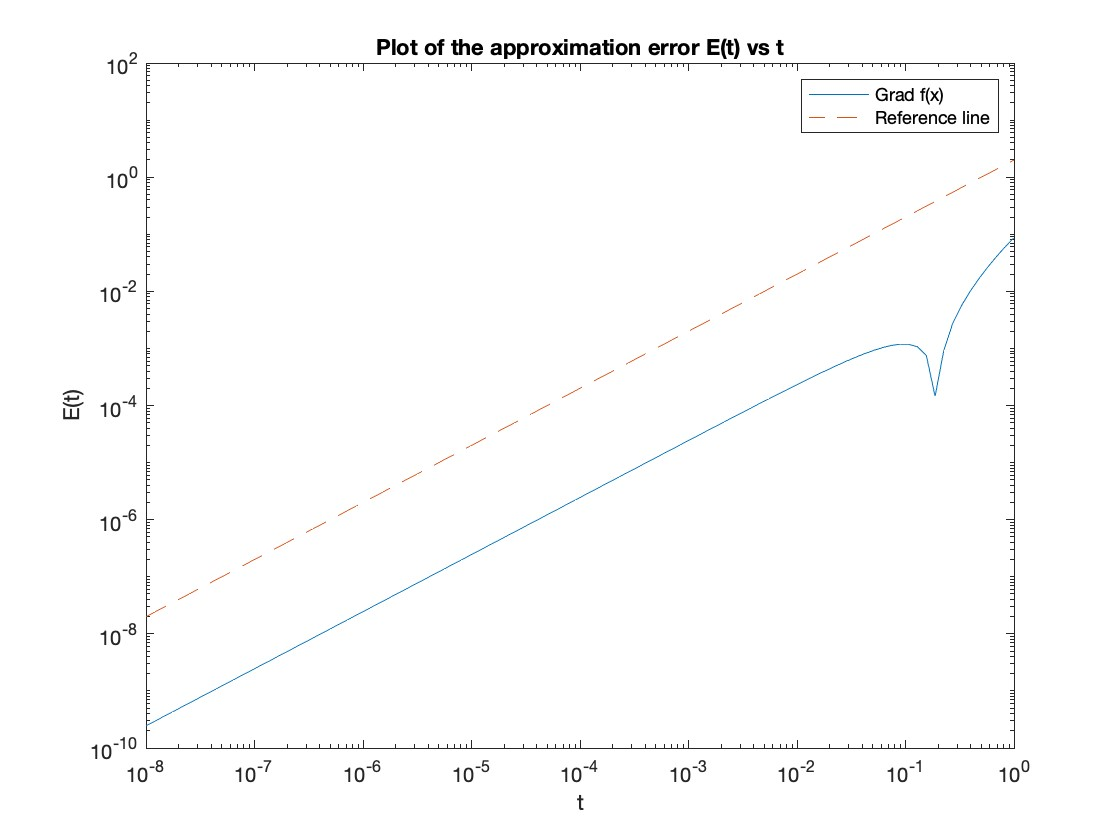
\includegraphics[width=12cm]{check_grad.jpg}
    \caption{Numerical check of the gradient via a comparison of the approximation error with a reference slope}
    \label{fig:check_grad}
\end{figure}

\subsection*{Question 11}
The backtracking line-search procedure for the choice of $\alpha$ is implemented in the following function, which follows Algorithm 4.2 of the textbook \cite{boumal2023intromanifolds}. It takes as input a point $X\in\text{OB}(d, n)$ and an initial parameter $\Bar{\alpha}>0$ and returns $\alpha$.\\
\begin{lstlisting}[style=Matlab-editor, numbers=left, frame=single, backgroundcolor=\color{gray!5}]
function alpha = BLS(X, alpha_bar)

% Initialization
tau = 0.5;
r = 1e-4;
alpha = alpha_bar;
[f, gradf] = Computefgradf(X, true);

while(f - Computefgradf(Retraction(X, -alpha*gradf), false) < r * alpha * Metric(gradf, gradf, X))
    alpha = tau * alpha;
end

end
\end{lstlisting}
The Riemannian gradient descent algorithm using a backtracking line-search procedure is then performed via the following function. The function takes as input an initial point $X_0\in\text{OB}(d, n)$, an initial value $\alpha_0$ for the parameter $\alpha$ and a maximal number of iterations \texttt{maxiter}. It returns the final position $X$, a boolean variable \texttt{conv} indicating whether the algorithm has converged before the maximal number of iterations or not, as well as the successive function values and gradient norms across iterations.\\
\begin{lstlisting}[style=Matlab-editor, numbers=left, frame=single, backgroundcolor=\color{gray!5}]
function [X, conv, f_values, grad_norm] = RGD_BLS(X0, alpha0, maxiter)

% Initialization
conv = false;
X = X0;
alpha = alpha0;
epsilon = 1e-6;

f_values = zeros(1, maxiter);
grad_norm = zeros(1, maxiter);

[~, gradf] = Computefgradf(X, true);

% RGD loop
for k = 1:maxiter

    X = Retraction(X, -alpha * gradf);

    [f, gradf] = Computefgradf(X, true);

    % Stock the function value and the gradient norm
    f_values(k) = f;
    grad_norm(k) = sqrt(Metric(gradf, gradf, X));

    % Control of convergence
    if sqrt(Metric(gradf, gradf, X)) < epsilon
        conv = true;
        fprintf('Riemannian Gradient Descent with backingtrack line-search did converge\n')
        fprintf('Final position:\n')
        disp(X)
        fprintf('Final function value:\n')
        disp(Computefgradf(X, false))
        fprintf('Number of iterations:\n')
        disp(k)
        break;
    end

    % Update alpha for next iteration
    alpha = BLS(X, alpha);
end

f_values = f_values(1:k);
grad_norm = grad_norm(1:k);

if conv == false
    fprintf('Riemannian Gradient Descent with backingtrack line-search did not converge\n')
    fprintf('Final position:\n')
    disp(X)
    fprintf('Final function value:\n')
    disp(Computefgradf(X, false))
end

end
\end{lstlisting}

\newpage

\section*{Experiments}
\addcontentsline{toc}{section}{\protect\numberline{}Experiments}

\subsection*{Question 12}
The following function, taking as inputs $d, n$, a maximal number of iterations \texttt{iter} and an initial value of $\alpha$ for the Riemannian gradient descent with backtracking line-search procedure, as well as a boolean variable \texttt{plots} indicating whether one wants the plots of the value functions and of the gradient norms to be displayed or not, performs the $30$ experiments for a given pair $(d, n)$ and returns additionally the final cost function values at each iteration as well as the best configuration obtained and corresponding iteration number. Namely, it displays the final positions, function values and number of iterations, as well as plots of the function values and gradient norms across iterations if required, for a given pair $(d, n)$, and returns a list of the final cost function values, together with the $X\in\text{OB}(d,n)$ that gave the smallest cost and the $i$ corresponding to the iteration number where the best configuration was obtained.\\
\begin{lstlisting}[style=Matlab-editor, numbers=left, frame=single, backgroundcolor=\color{gray!5}]
function [final_costs, X_best, i_best] = Experiments(d, n, iter, alpha, plots)

final_costs = zeros(1, 30);

for i = 1:30
    X0 = SampleOB(d, n);
    [X, ~, f_values, grad_norm] = RGD_BLS(X0, alpha, iter);
    final_costs(i) = f_values(length(f_values));

    if i == 1
        X_best = X;
        i_best = i;
    elseif final_costs(i) < min(final_costs(1:i-1))
        X_best = X;
        i_best = i;
    end

    if plots
        % Plot function value as function of iterations
        figure;
        plot(1:length(f_values), f_values, '-o', 'LineWidth', 2);
        xlabel('Iterations');
        ylabel('Value f(x)');
        title(sprintf('Convergence of f(x) for n = %.2f', n));
        grid on;

        % Plot gradient norm (on log scale) as function of iterations
        figure;
        plot(1:length(grad_norm), log(grad_norm), '-o', 'LineWidth', 2);
        xlabel('Iterations');
        ylabel('Norm of gradf(x) (log scale)');
        title(sprintf('Decay of the norm of gradf(x) (log scale) for n = %.2f', n));
        grid on;
    end

end

end
\end{lstlisting}
We then perform the experiments for each required pair. Table \ref{tab:d2} depicts the smallest and largest cost function values we obtained among the $30$ iterations, for each pair $(d, n)$ for $d=2$.
\begin{table}[H]
\centering
\begin{tabular}{|c|c|c|}
\hline
$n$ & Minimum & Maximum \\ \hline
3 & -0.4055 & -0.4055 \\
4 & -0.2310 & -0.2310 \\
5 & -0.1116 & -0.1116 \\
6 & -0.0236 & -0.0236 \\
20 & 0.3778 & 0.3778 \\
100 & 0.6001 & 0.6005 \\
\end{tabular}
\caption{Smallest and largest cost function values for $d=2$ and a maximum of $250$ iterations in the RGD with initial $\alpha$ equal to $1$}
\label{tab:d2}
\end{table}
We observe that for $n=100$ the minimum and maximum values differ. This occurs because the algorithm has not converged after $250$ iterations in this case. Nevertheless, the difference between both values is not very large, being of the order of $10^{-4}$. Moreover, we notice that as $n$ increases, the cost function value increases. This occurs because as $n$ increases, the points on the circle lie closer to each other, resulting in an increase of $f$.\\
Table \ref{tab:d3} shows the minimum and maximum values attained for $d=3$.
\begin{table}[H]
\centering
\begin{tabular}{|c|c|c|}
\hline
$n$ & Minimum & Maximum \\ \hline
2 & -0.6931 & -0.6931 \\
3 & -0.4055 & -0.4055 \\
4 & -0.2877 & -0.2877 \\
5 & -0.1910 & -0.1899 \\
6 & -0.1386 & -0.1382 \\
12 & 0.0385 & 0.0430 \\
16 & 0.0916 & 0.0948 \\
50 & 0.2181 & 0.2191 \\
128 & 0.2663 & 0.2672 \\
\end{tabular}
\caption{Smallest and largest cost function values for $d=3$ and a maximum of $250$ iterations in the RGD with initial $\alpha$ equal to $1$}
\label{tab:d3}
\end{table}
The conclusions are similar to the case $d=2$. As $n$ increases, the smallest and largest values start to differ, but are still close to each other. Also, the value of $f$ increases as $n$ increases, as the distance between the points gets smaller when the number of points increases. We furthermore notice that the final function value for the pair $(3, 3)$ is the same as the one we obtained for the pair $(2, 3)$. This occurs because the optimal configuration for $(2, 3)$ is an equilateral triangle, just as for $(3, 3)$, and thus the distances between the points are the same in these two cases.\\
\newline
We now visualize the optimal configurations for each pair $(d, n)$. Up to rotation, the algorithm converged to the same spread of the points. Figure \ref{fig:opt2_group} illustrates the best configurations obtained for $d=2$ and $n\in\{3, 4, 5, 6, 20, 100\}$. As expected, the points are spread on the circle so as to be as far from each other as possible.
\begin{figure}[H]
    \centering
    \begin{subfigure}[b]{0.32\textwidth}
        \centering
        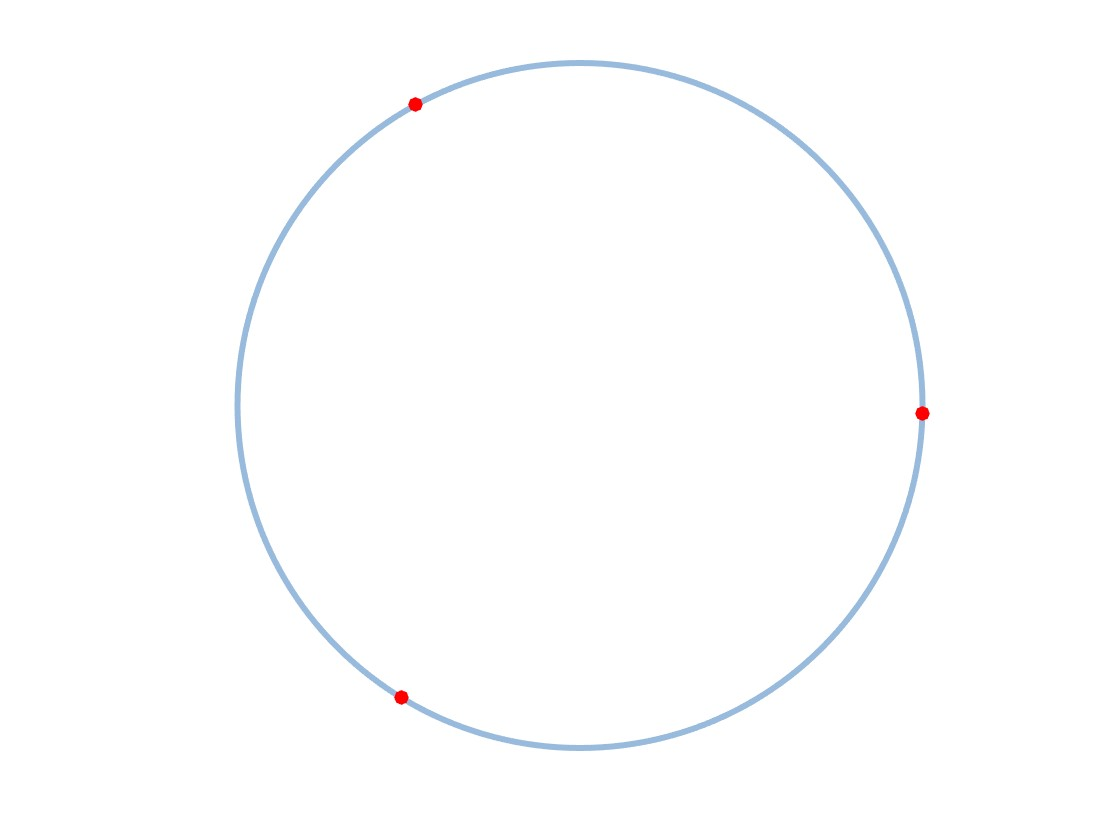
\includegraphics[width=\textwidth]{opt2_3.jpg}
        \caption{Pair (2,3)}
        \label{fig:opt2_3}
    \end{subfigure}
    \begin{subfigure}[b]{0.32\textwidth}
        \centering
        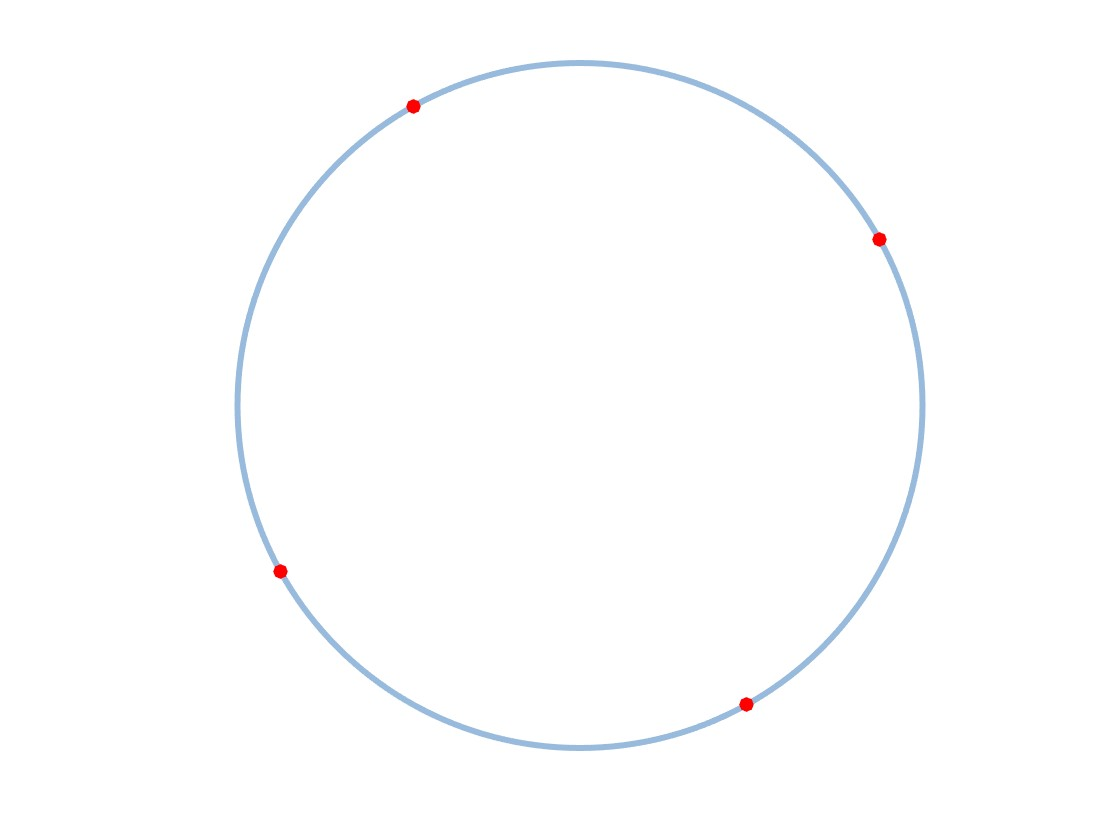
\includegraphics[width=\textwidth]{opt2_4.jpg}
        \caption{Pair (2,4)}
        \label{fig:opt2_4}
    \end{subfigure}
    \begin{subfigure}[b]{0.32\textwidth}
        \centering
        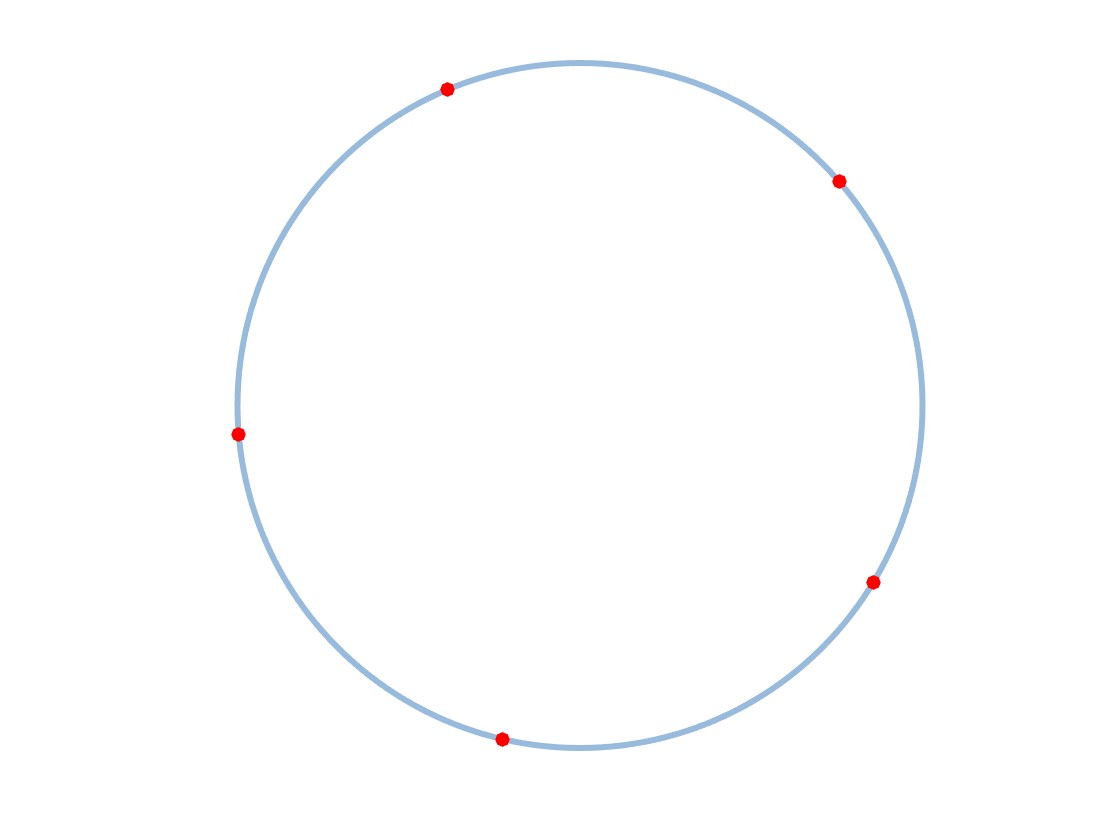
\includegraphics[width=\textwidth]{opt2_5.jpg}
        \caption{Pair (2,5)}
        \label{fig:opt2_5}
    \end{subfigure}
    
    \begin{subfigure}[b]{0.32\textwidth}
        \centering
        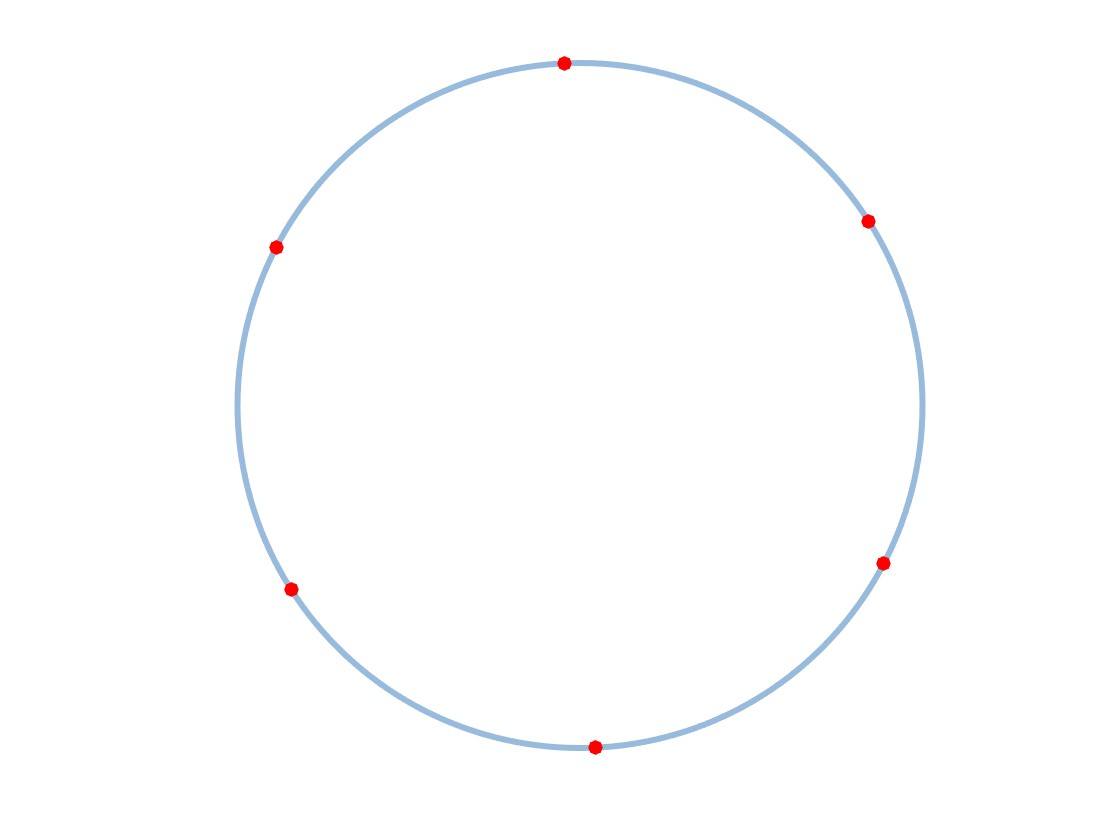
\includegraphics[width=\textwidth]{opt2_6.jpg}
        \caption{Pair (2,6)}
        \label{fig:opt2_6}
    \end{subfigure}
    \begin{subfigure}[b]{0.32\textwidth}
        \centering
        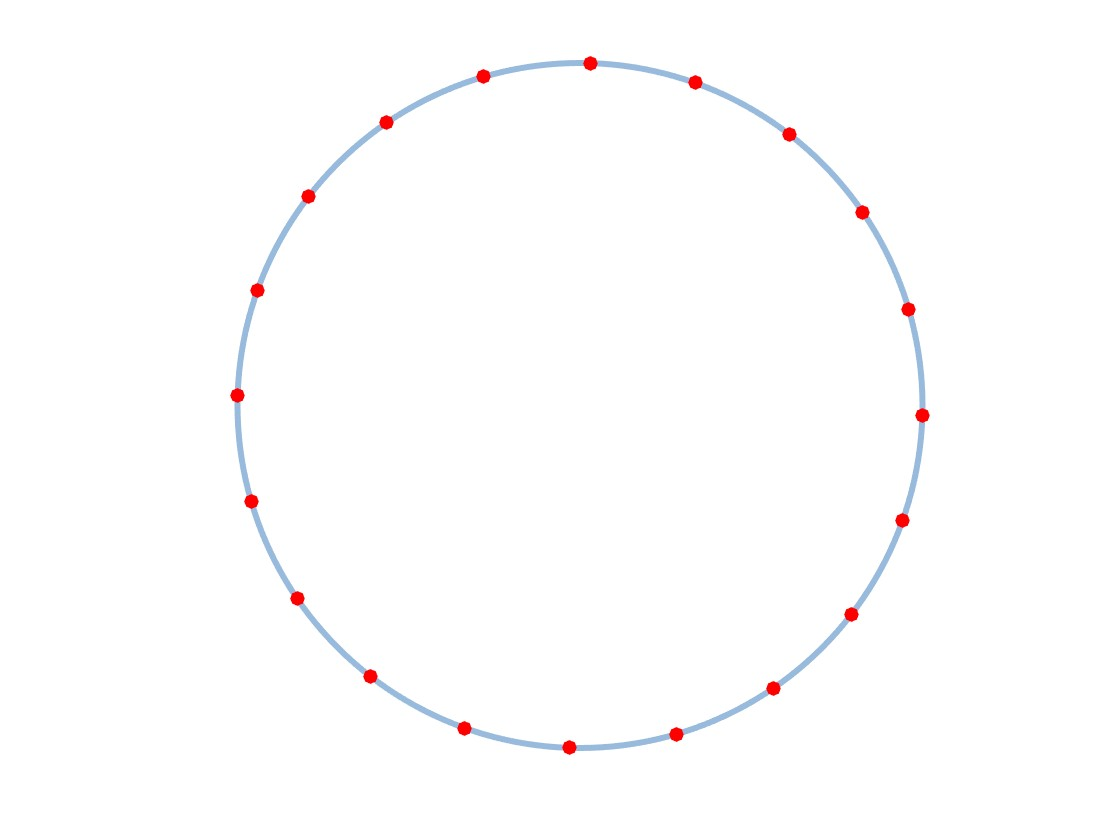
\includegraphics[width=\textwidth]{opt2_20.jpg}
        \caption{Pair (2,20)}
        \label{fig:opt2_20}
    \end{subfigure}
    \begin{subfigure}[b]{0.32\textwidth}
        \centering
        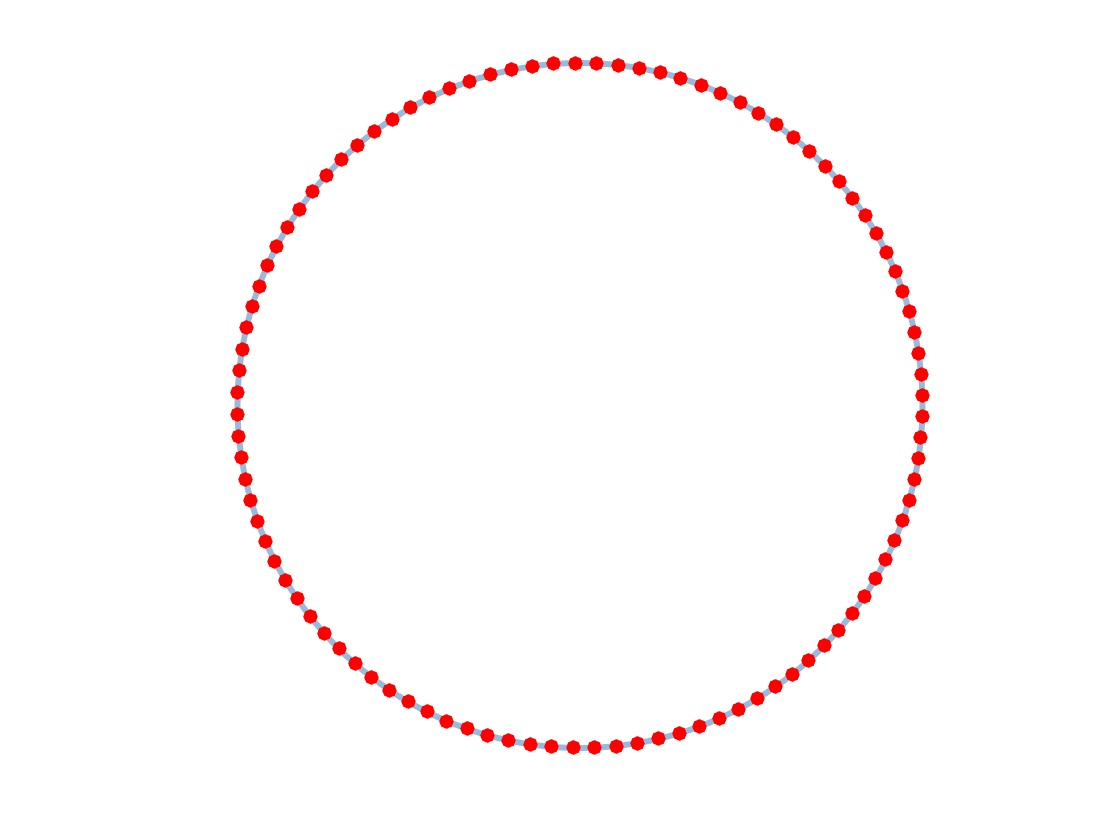
\includegraphics[width=\textwidth]{opt2_100.jpg}
        \caption{Pair (2,100)}
        \label{fig:opt2_100}
    \end{subfigure}

    \caption{Optimal configurations for pairs $(2, n)$}
    \label{fig:opt2_group}
\end{figure}
Figure \ref{fig:opt3_group} illustrates the best configurations obtained for $d=3$. Up to rotation, the algorithm converged to the same spread of the points. For $n\leq 6$, we notice that the points seem to be as far from each other as possible, as desired. For higher values of $n$, as Table \ref{tab:d3} suggested, the algorithm has not converged due to the maximal number of iterations being attained before an enough decrease of the gradient norm. As a consequence, we notice that the points are not completely well-distributed on the surface of the sphere. Nonetheless, we see a tendency of the points to start lying apart from each other.
\begin{figure}[H]
    \centering
    \begin{subfigure}[b]{0.32\textwidth}
        \centering
        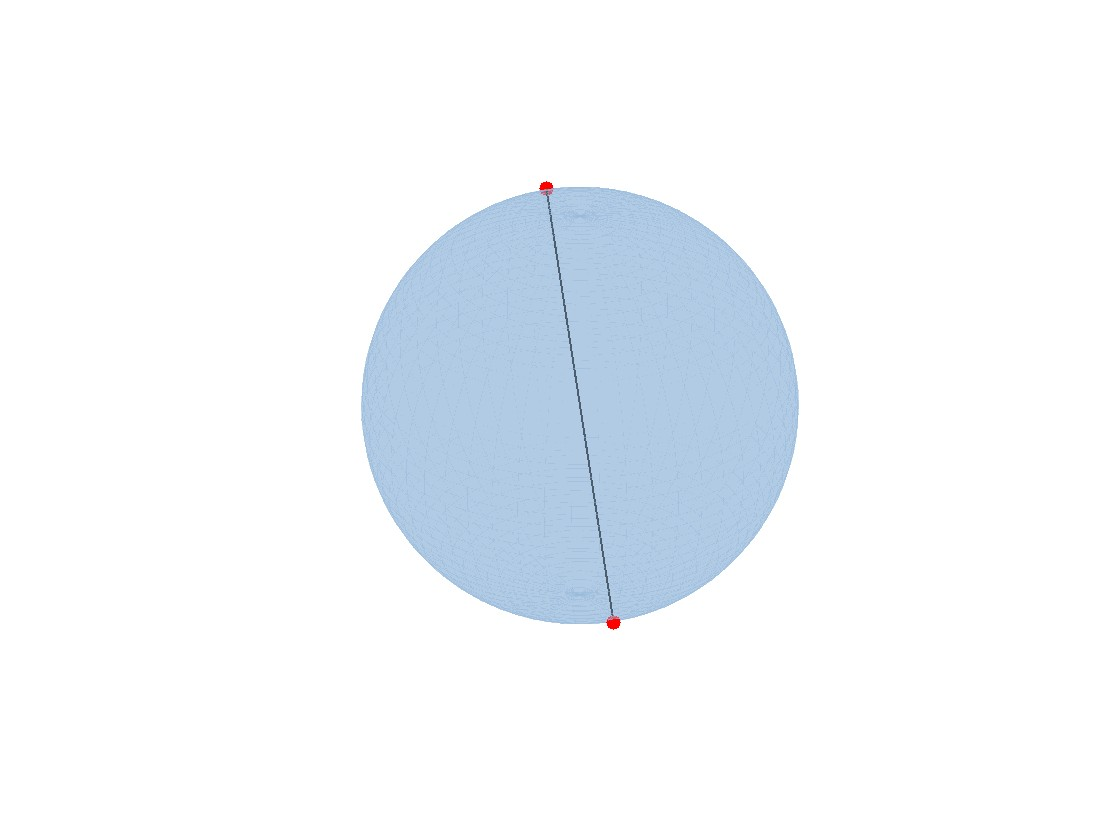
\includegraphics[width=\textwidth]{opt3_2.jpg}
        \caption{Pair (3,2)}
        \label{fig:opt3_2}
    \end{subfigure}
    \begin{subfigure}[b]{0.32\textwidth}
        \centering
        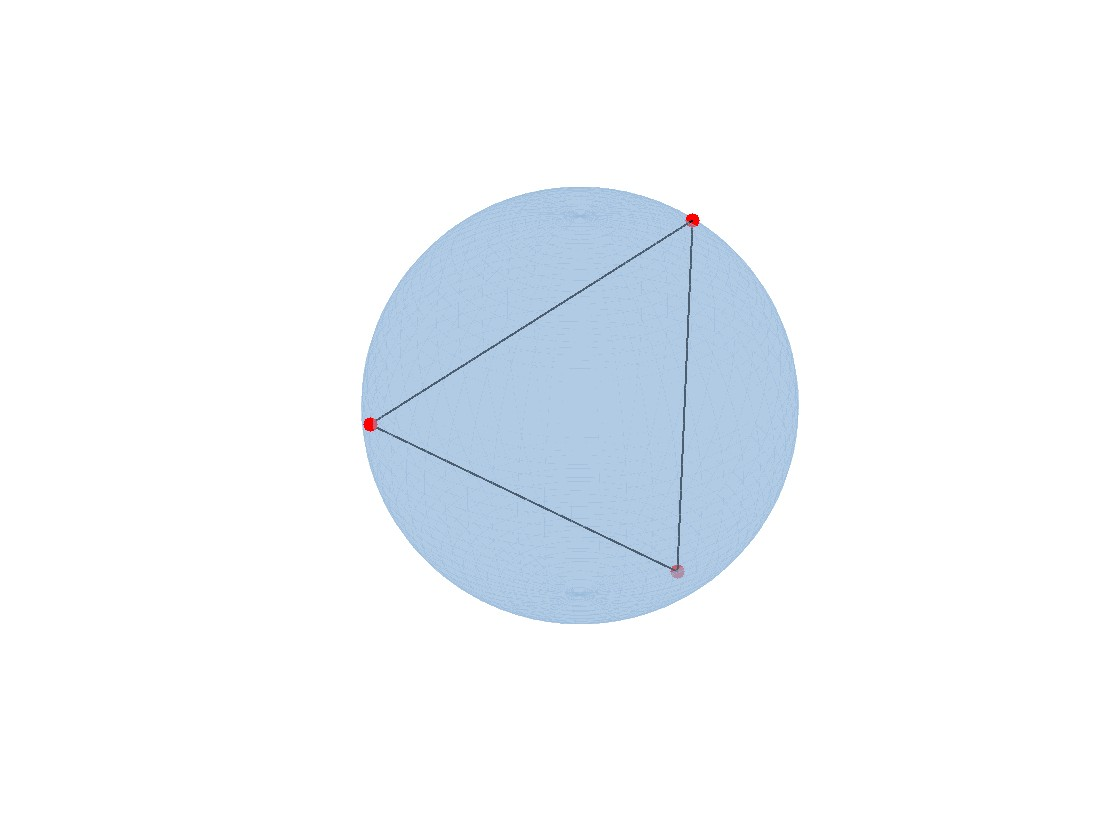
\includegraphics[width=\textwidth]{opt3_3.jpg}
        \caption{Pair (3,3)}
        \label{fig:opt3_3}
    \end{subfigure}
    \begin{subfigure}[b]{0.32\textwidth}
        \centering
        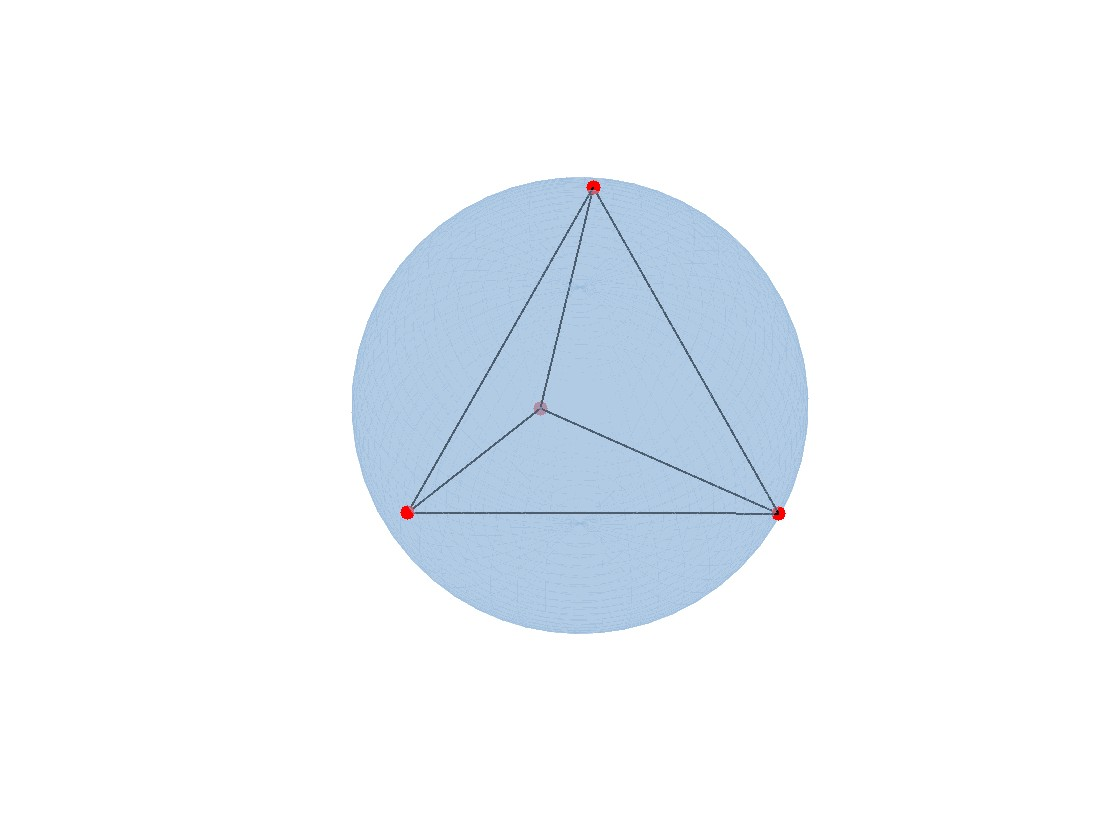
\includegraphics[width=\textwidth]{opt3_4.jpg}
        \caption{Pair (3,4)}
        \label{fig:opt3_4}
    \end{subfigure}
    
    \begin{subfigure}[b]{0.32\textwidth}
        \centering
        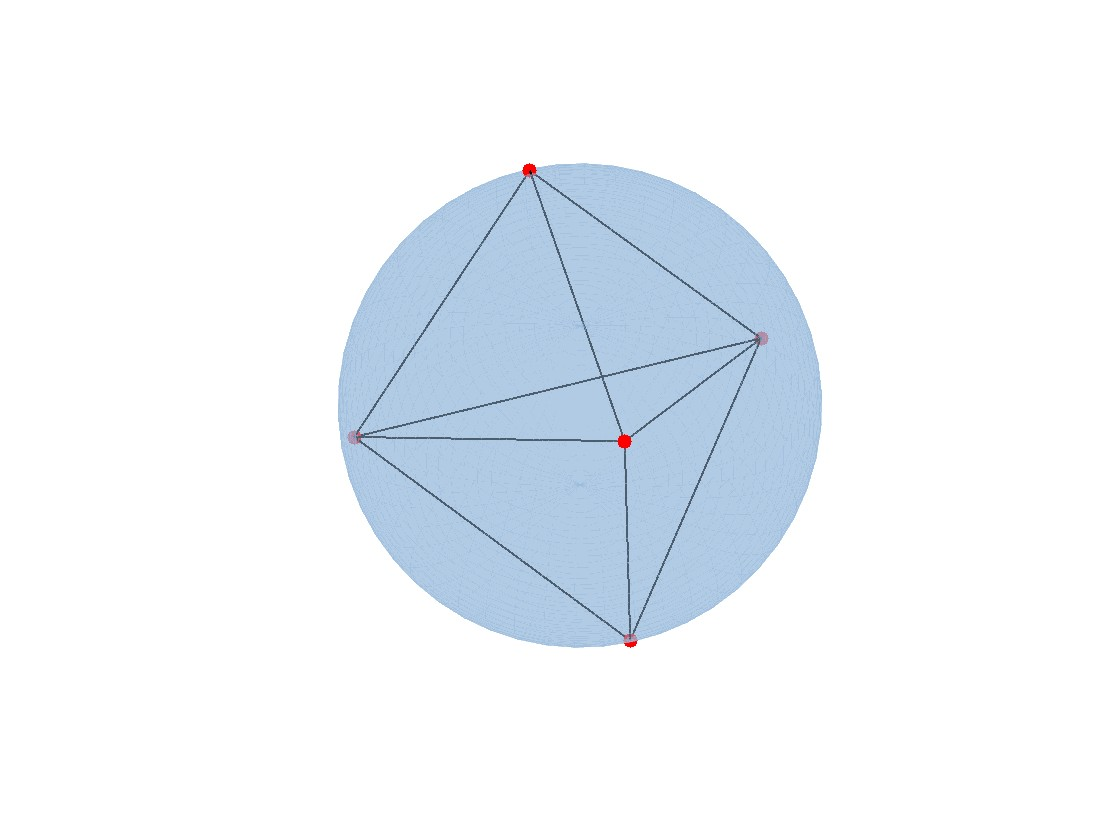
\includegraphics[width=\textwidth]{opt3_5.jpg}
        \caption{Pair (3,5)}
        \label{fig:opt3_5}
    \end{subfigure}
    \begin{subfigure}[b]{0.32\textwidth}
        \centering
        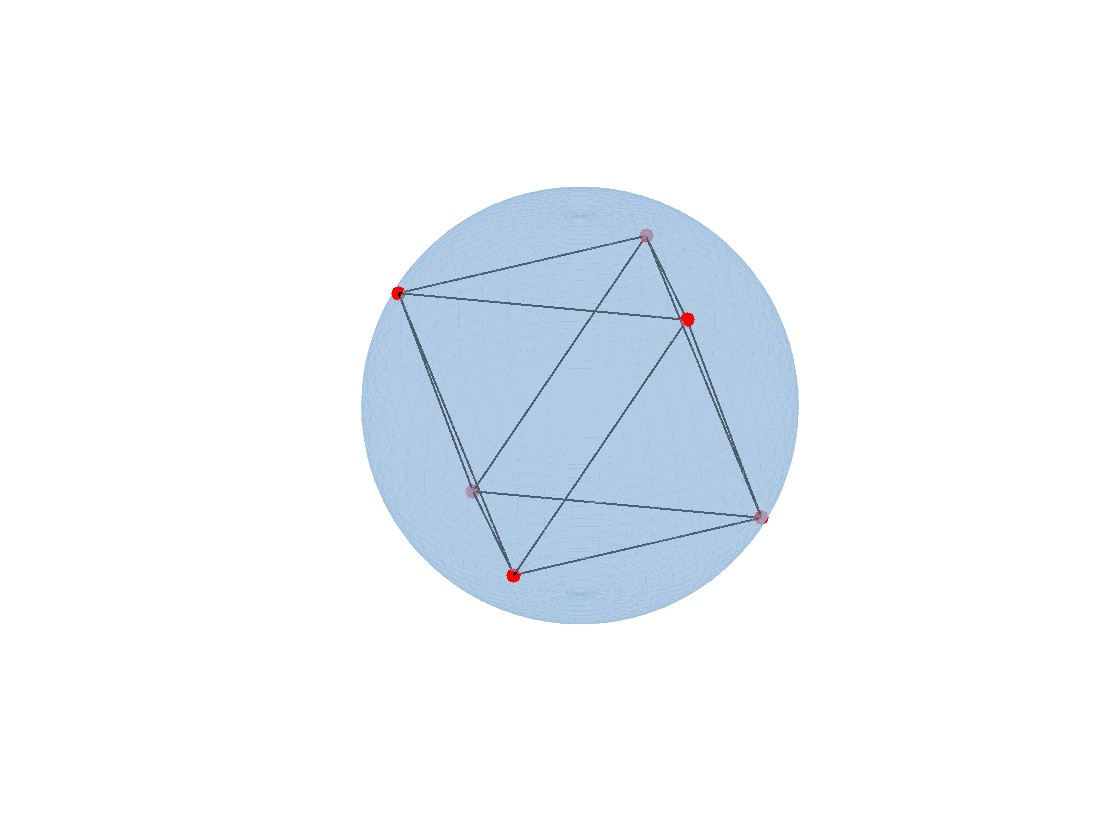
\includegraphics[width=\textwidth]{opt3_6.jpg}
        \caption{Pair (3,6)}
        \label{fig:opt3_6}
    \end{subfigure}
    \begin{subfigure}[b]{0.32\textwidth}
        \centering
        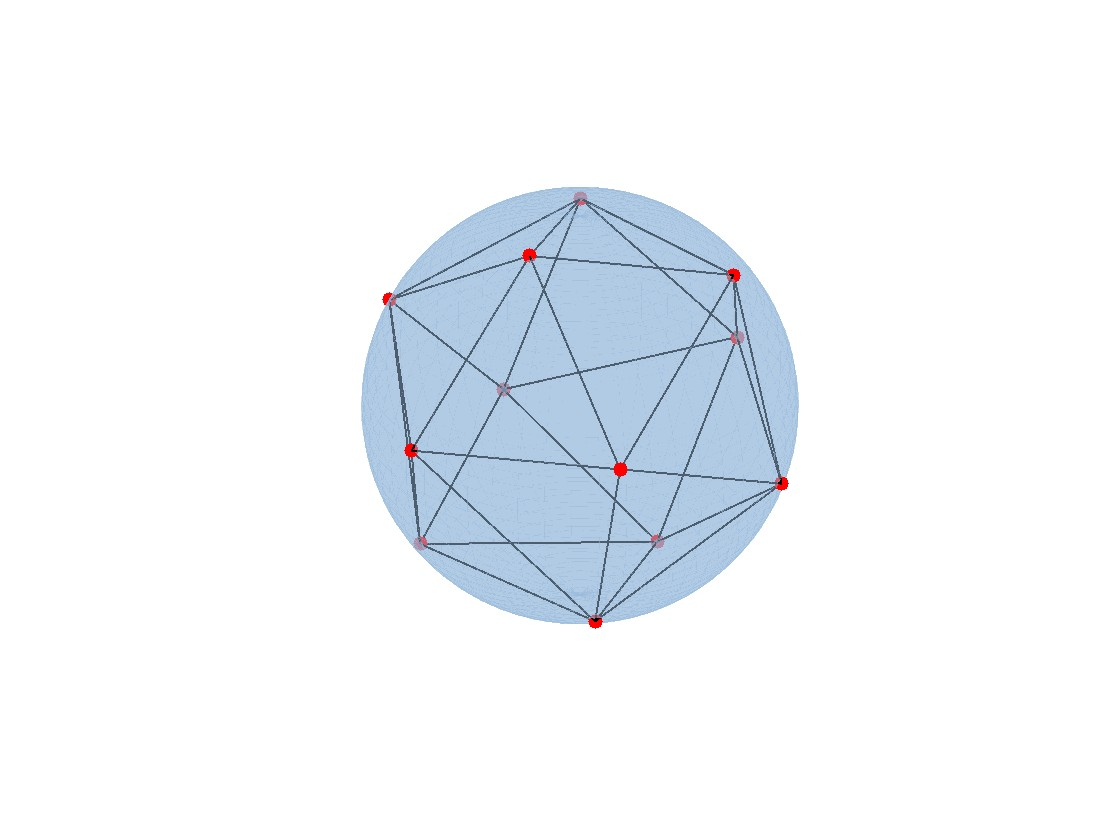
\includegraphics[width=\textwidth]{opt3_12.jpg}
        \caption{Pair (3,12)}
        \label{fig:opt3_12}
    \end{subfigure}

    \begin{subfigure}[b]{0.32\textwidth}
        \centering
        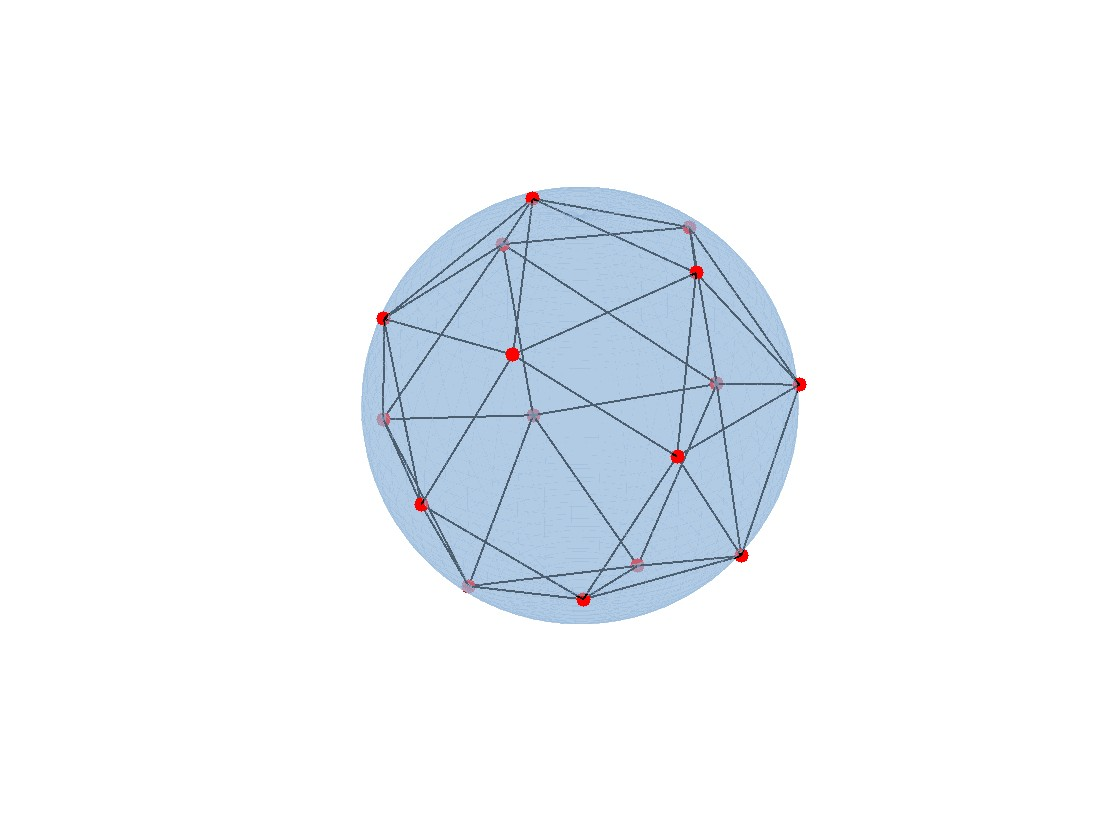
\includegraphics[width=\textwidth]{opt3_16.jpg}
        \caption{Pair (3,16)}
        \label{fig:opt3_16}
    \end{subfigure}
    \begin{subfigure}[b]{0.32\textwidth}
        \centering
        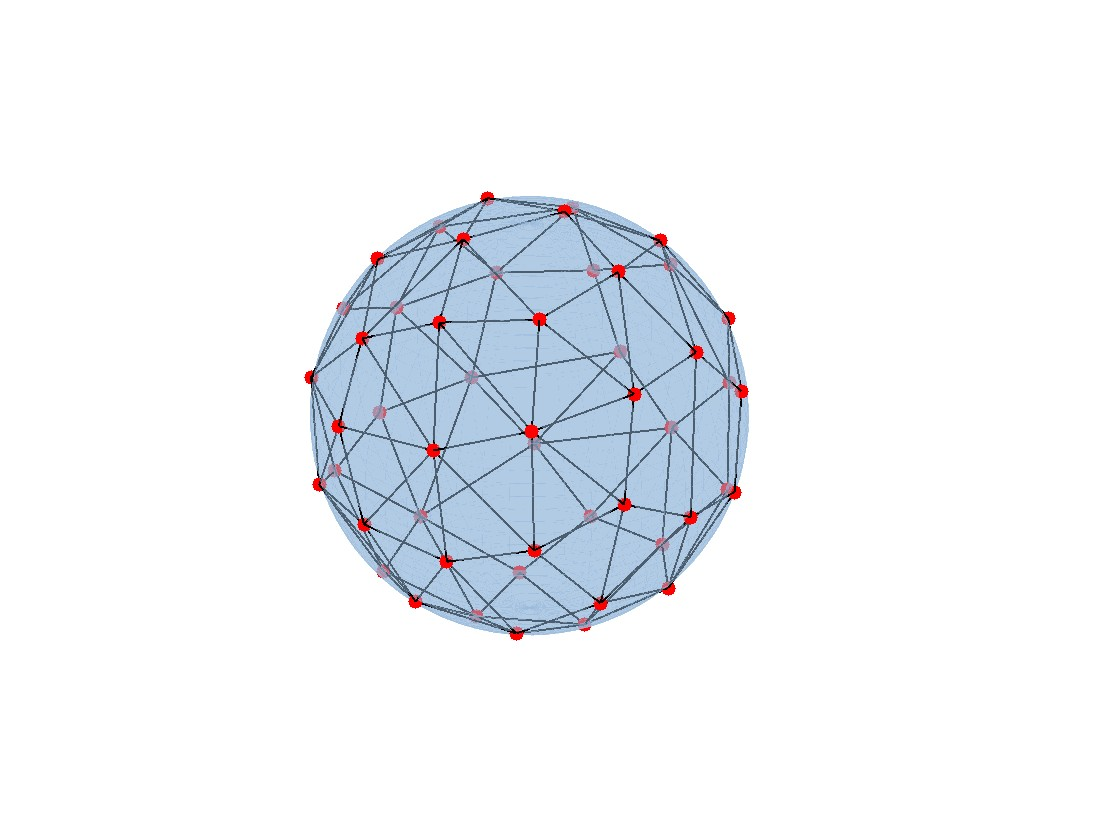
\includegraphics[width=\textwidth]{opt3_50.jpg}
        \caption{Pair (3,50)}
        \label{fig:opt3_50}
    \end{subfigure}
    \begin{subfigure}[b]{0.32\textwidth}
        \centering
        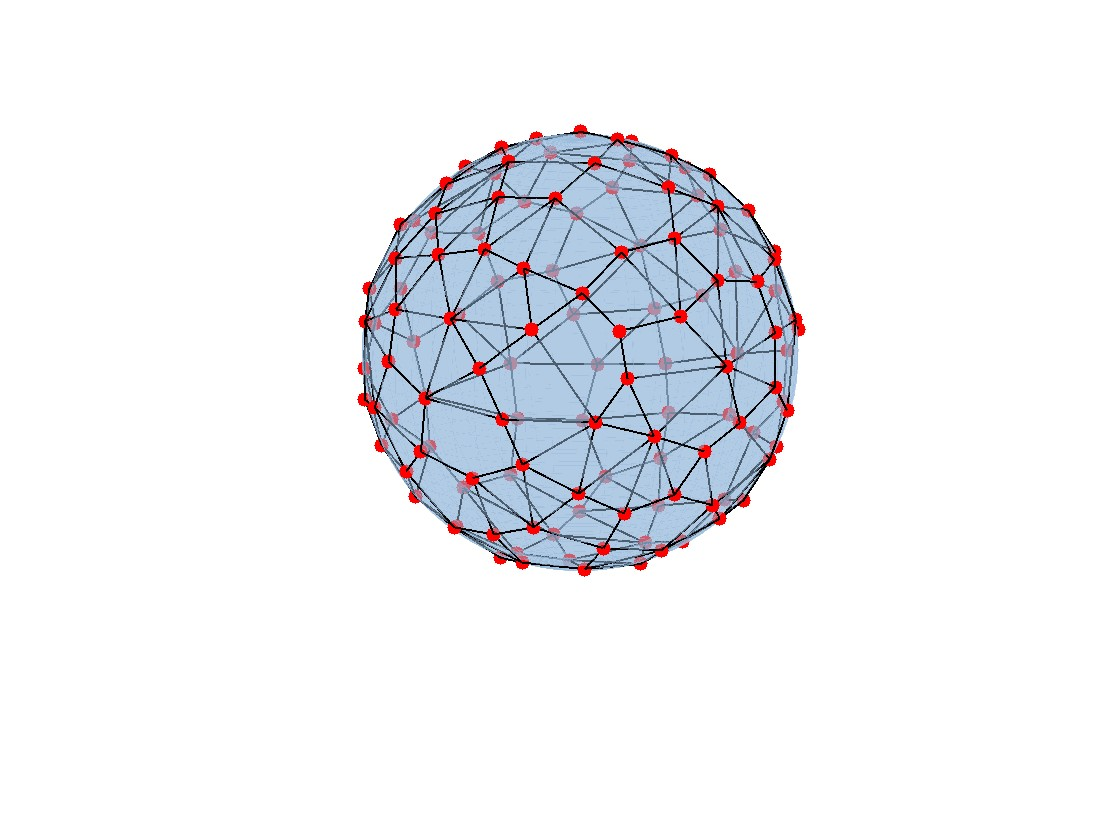
\includegraphics[width=\textwidth]{opt3_128.jpg}
        \caption{Pair (3,128)}
        \label{fig:opt3_128}
    \end{subfigure}

    \caption{Optimal configurations for pairs $(3, n)$}
    \label{fig:opt3_group}
\end{figure}
We now proceed to show the substantially different configurations we obtain until convergence, to understand how the algorithm gets closer to the optimal solution, and compare them to the best configurations we obtained. Figures \ref{fig:conf2_3}, \ref{fig:conf2_4}, \ref{fig:conf2_5} and \ref{fig:conf2_6} give the visualizations after different numbers of iterations for the cases $d=2$ and $n\in\{3, 4, 5, 6\}$. We notice that as the number of iterations increases, the points move further apart, until reaching the optimal configuration where the distance between the points is maximized. For smaller $n$, less iterations are needed until convergence.

\begin{figure}[H]
    \centering
    \begin{subfigure}[b]{0.32\textwidth}
        \centering
        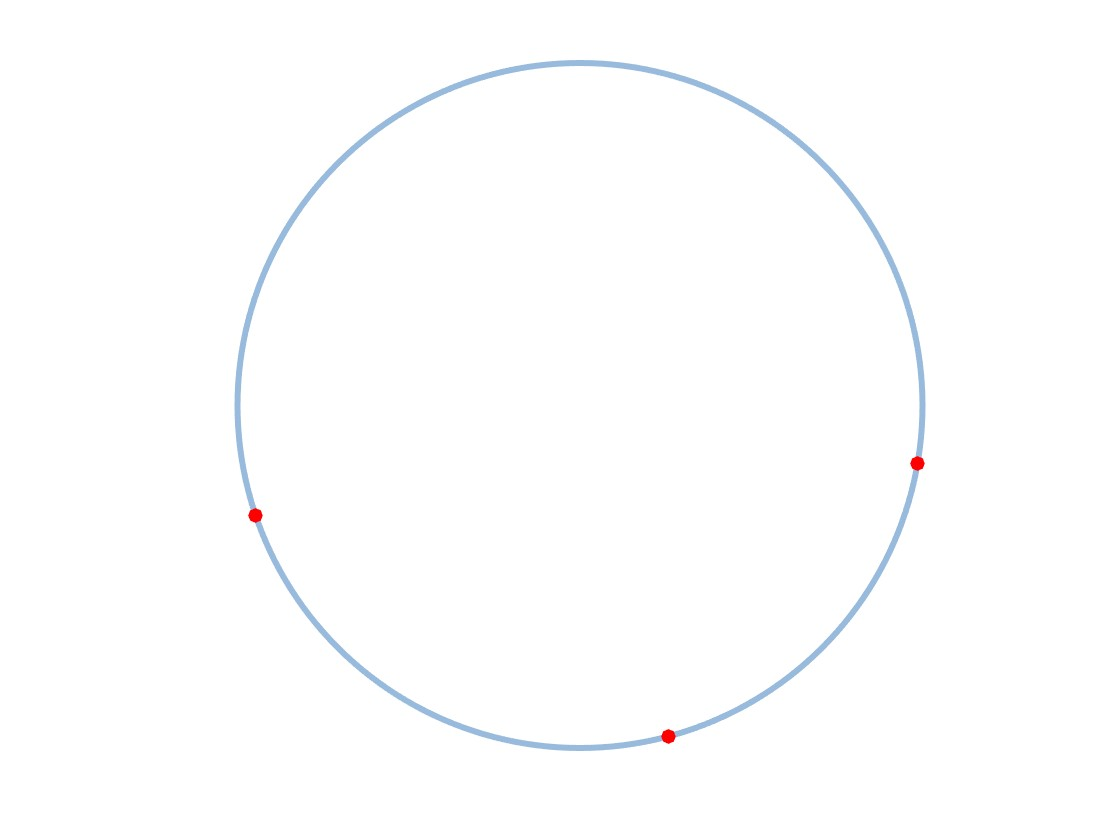
\includegraphics[width=\textwidth]{conf2_3_1.jpg}
        \caption{After $1$ iteration}
    \end{subfigure}
    \begin{subfigure}[b]{0.32\textwidth}
        \centering
        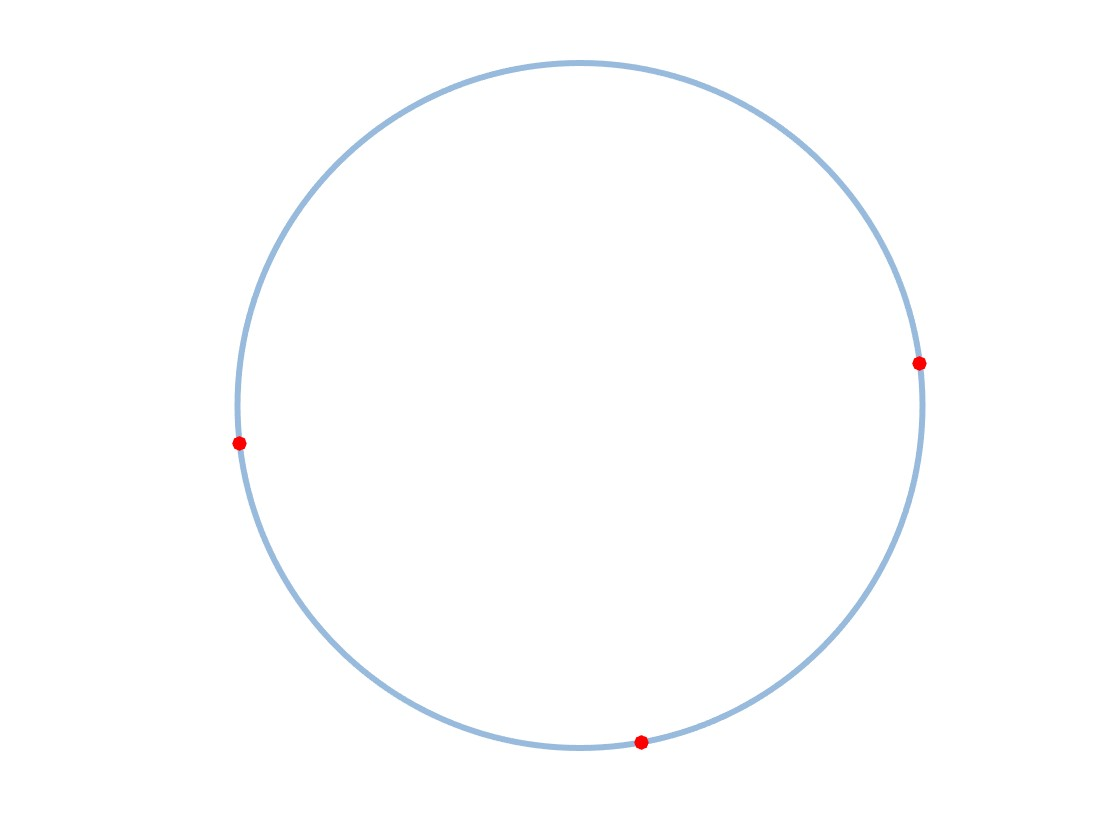
\includegraphics[width=\textwidth]{conf2_3_2.jpg}
        \caption{After $2$ iterations}
    \end{subfigure}

    \begin{subfigure}[b]{0.32\textwidth}
        \centering
        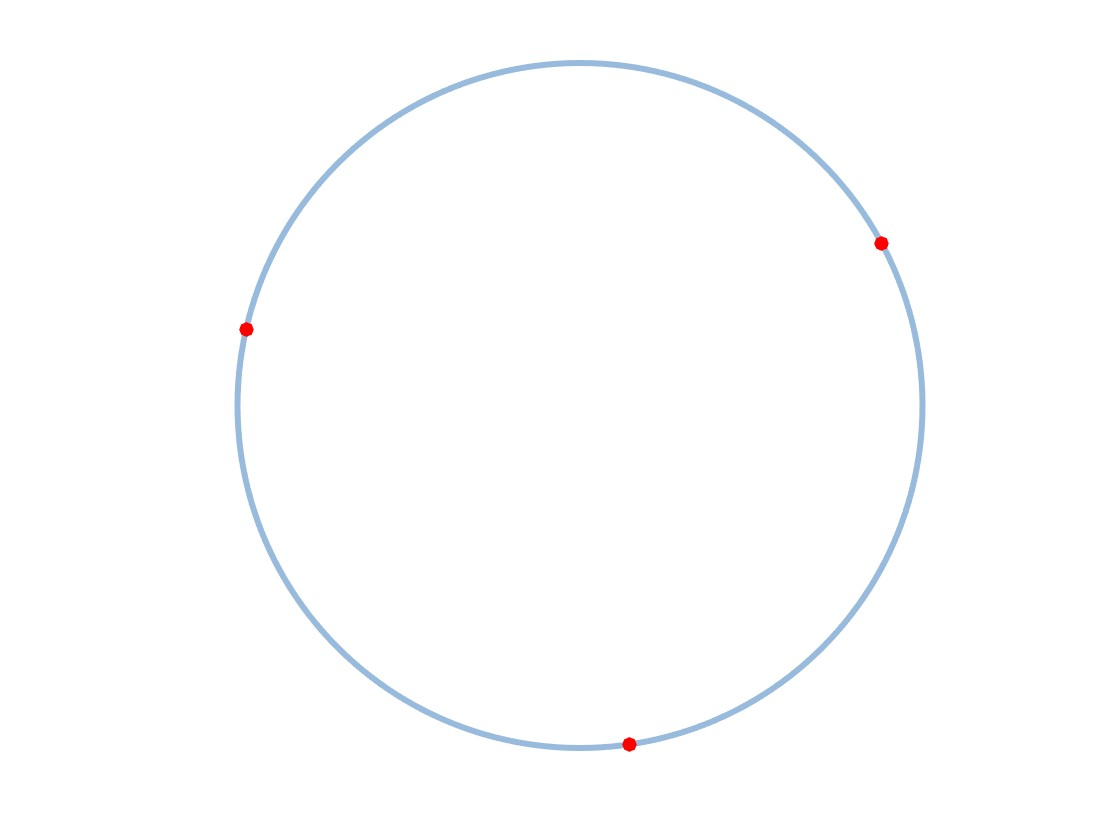
\includegraphics[width=\textwidth]{conf2_3_5.jpg}
        \caption{After $5$ iterations}
    \end{subfigure}
    \begin{subfigure}[b]{0.32\textwidth}
        \centering
        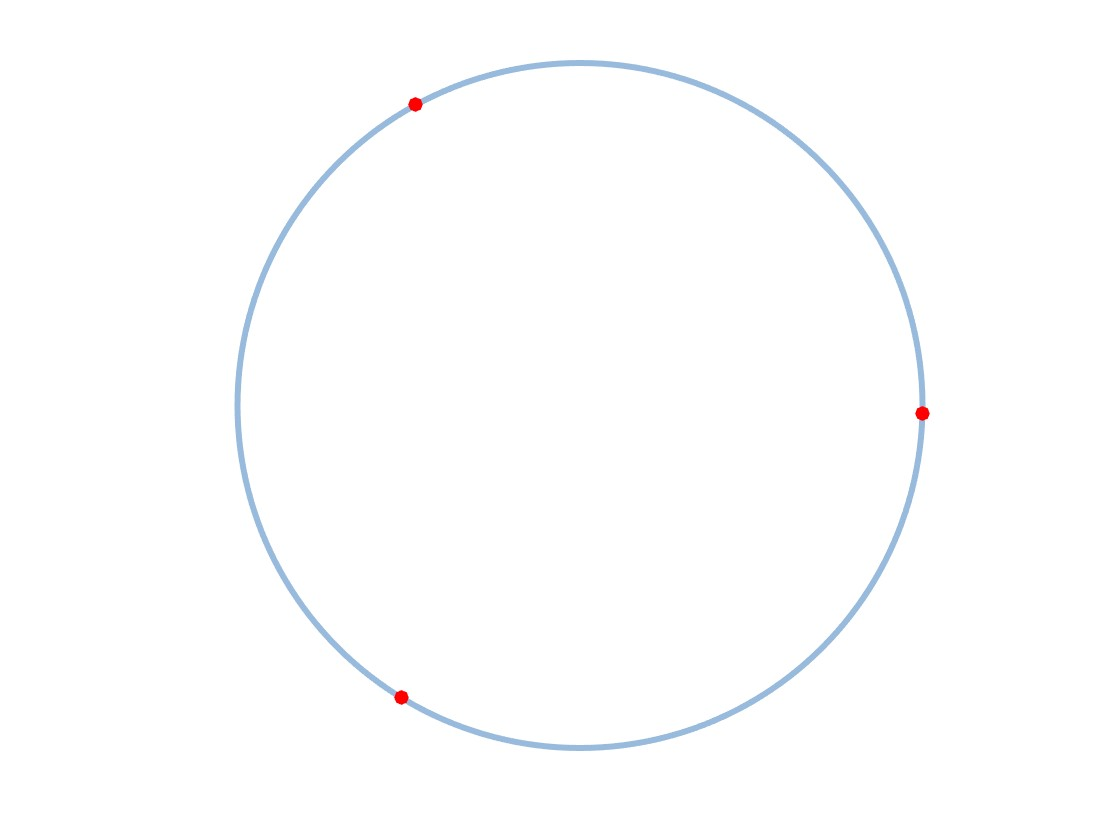
\includegraphics[width=\textwidth]{opt2_3.jpg}
        \caption{Best configuration obtained}
    \end{subfigure}

    \caption{Different configurations for $(2, 3)$}
    \label{fig:conf2_3}
\end{figure}




\begin{figure}[H]
    \centering
    \begin{subfigure}[b]{0.32\textwidth}
        \centering
        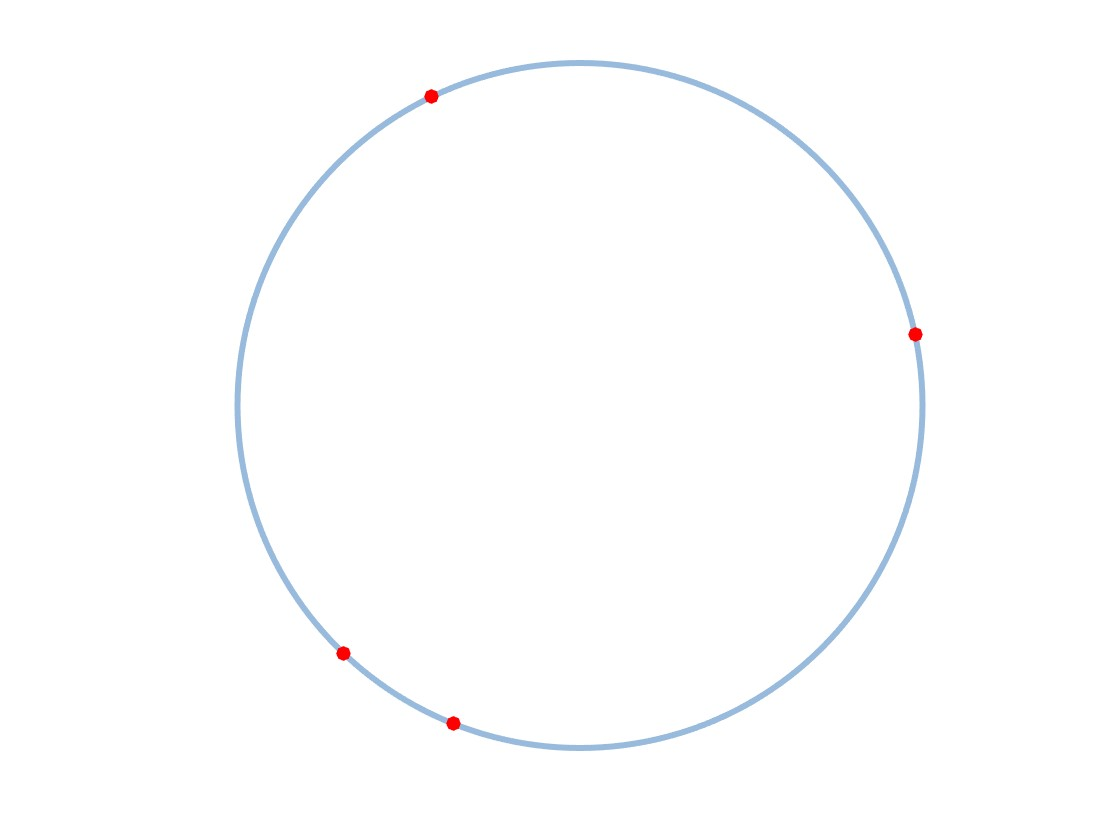
\includegraphics[width=\textwidth]{conf2_4_1.jpg}
        \caption{After $1$ iteration}
    \end{subfigure}
    \begin{subfigure}[b]{0.32\textwidth}
        \centering
        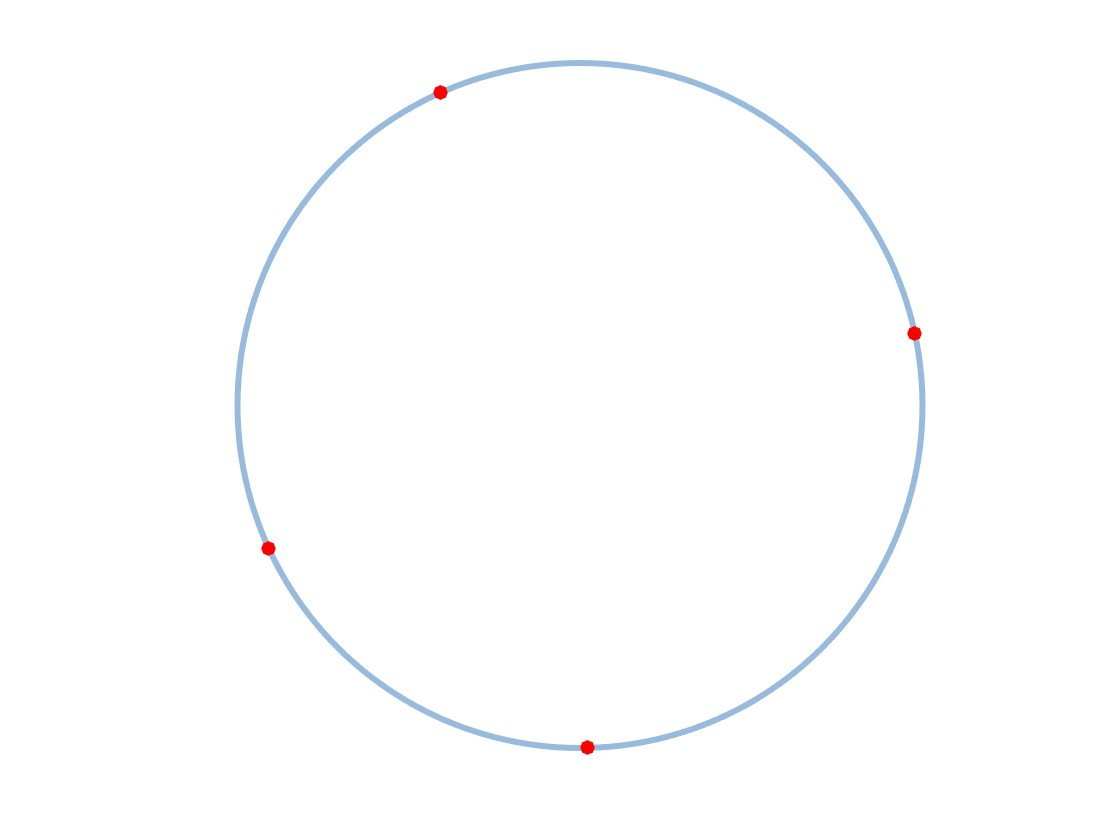
\includegraphics[width=\textwidth]{conf2_4_2.jpg}
        \caption{After $2$ iterations}
    \end{subfigure}

    \begin{subfigure}[b]{0.32\textwidth}
        \centering
        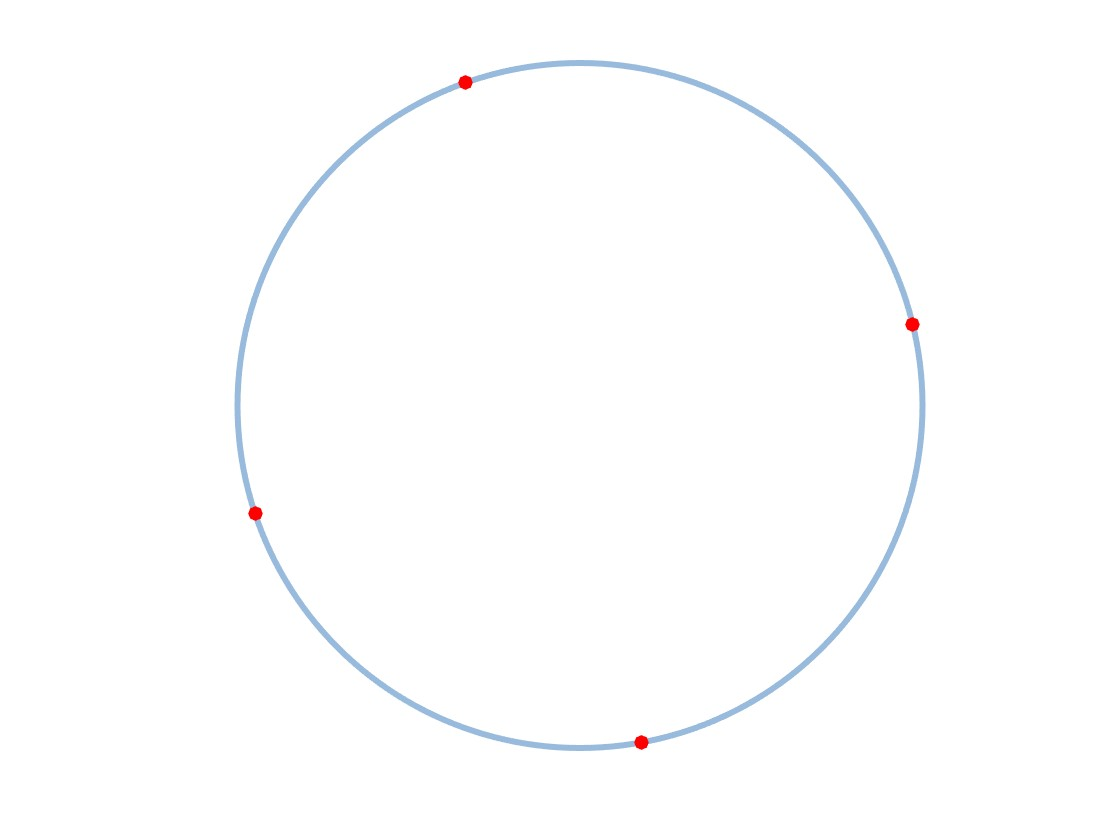
\includegraphics[width=\textwidth]{conf2_4_5.jpg}
        \caption{After $5$ iterations}
    \end{subfigure}
    \begin{subfigure}[b]{0.32\textwidth}
        \centering
        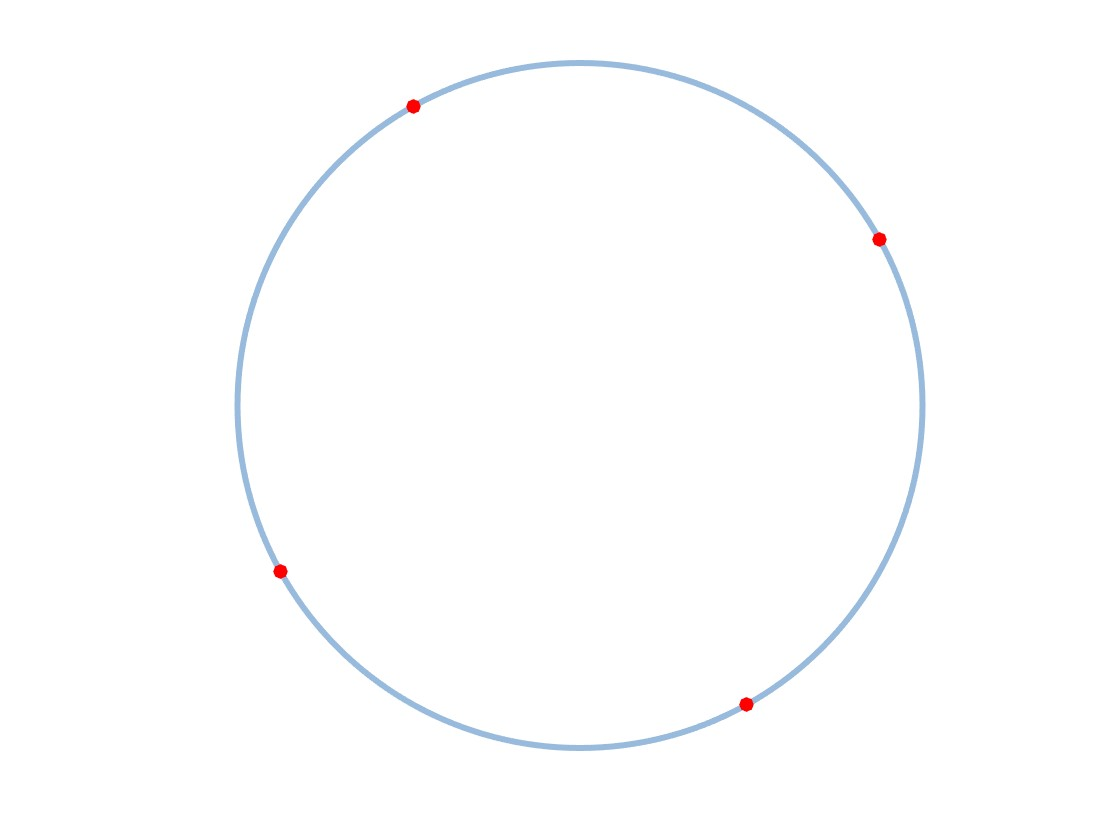
\includegraphics[width=\textwidth]{opt2_4.jpg}
        \caption{Best configuration obtained}
    \end{subfigure}

    \caption{Different configurations for $(2, 4)$}
    \label{fig:conf2_4}
\end{figure}



\begin{figure}[H]
    \centering
    \begin{subfigure}[b]{0.32\textwidth}
        \centering
        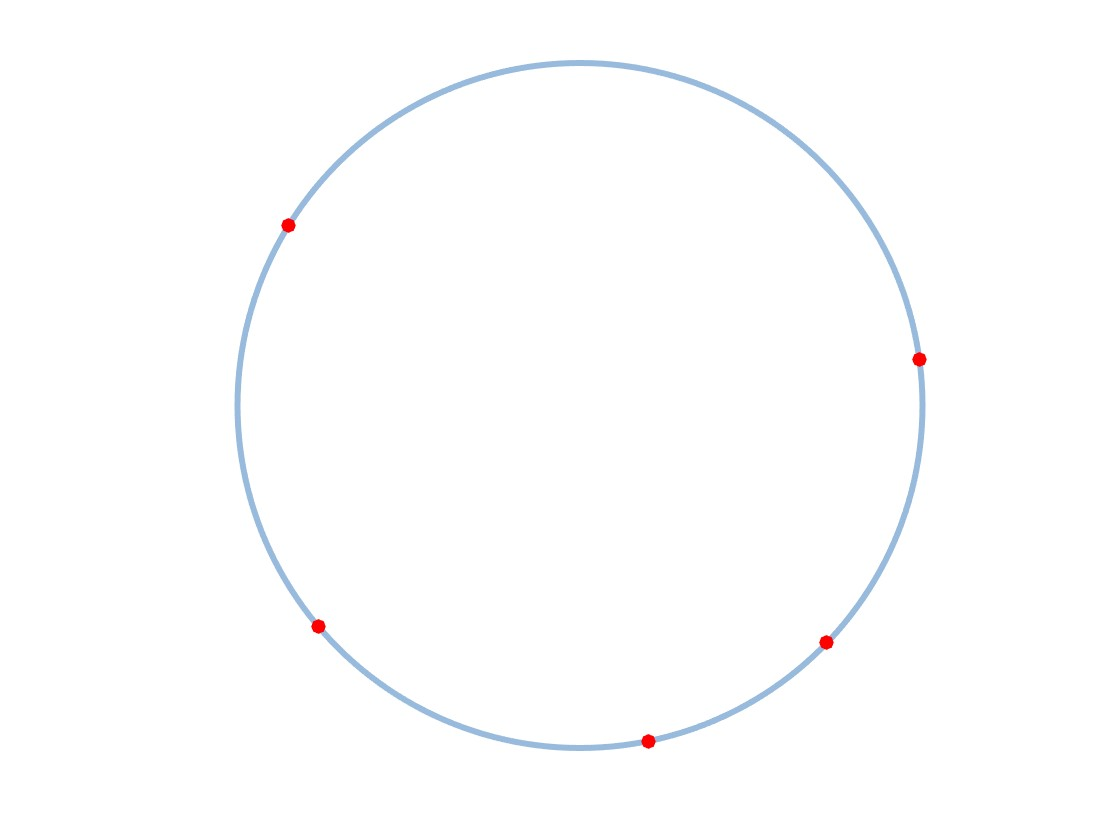
\includegraphics[width=\textwidth]{conf2_5_1.jpg}
        \caption{After $1$ iteration}
    \end{subfigure}
    \begin{subfigure}[b]{0.32\textwidth}
        \centering
        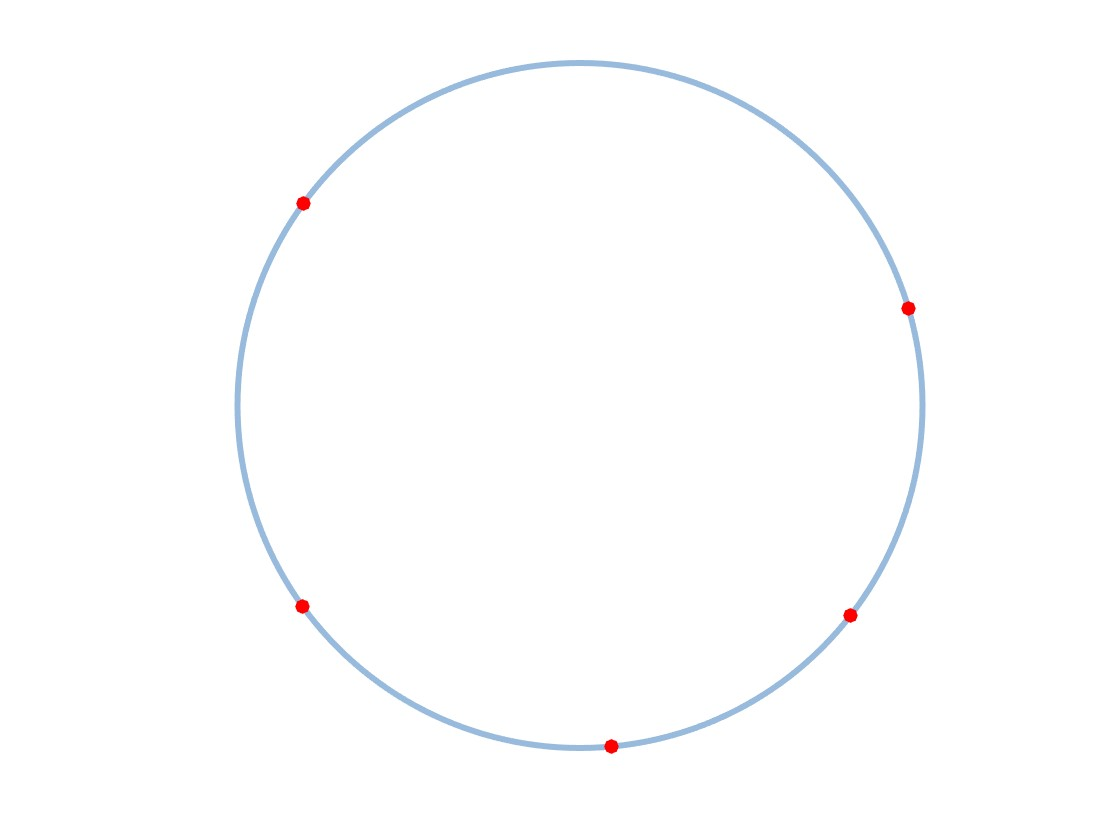
\includegraphics[width=\textwidth]{conf2_5_2.jpg}
        \caption{After $2$ iterations}
    \end{subfigure}
    \begin{subfigure}[b]{0.32\textwidth}
        \centering
        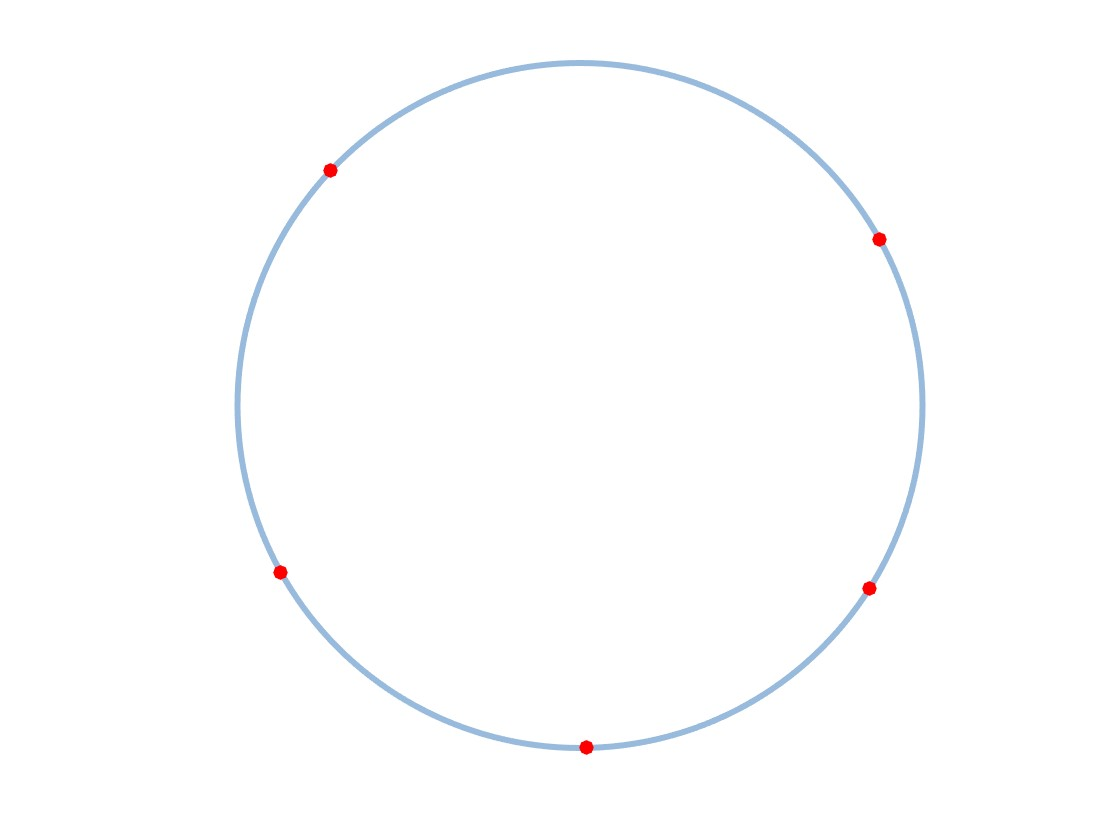
\includegraphics[width=\textwidth]{conf2_5_4.jpg}
        \caption{After $4$ iterations}
    \end{subfigure}

    \begin{subfigure}[b]{0.32\textwidth}
        \centering
        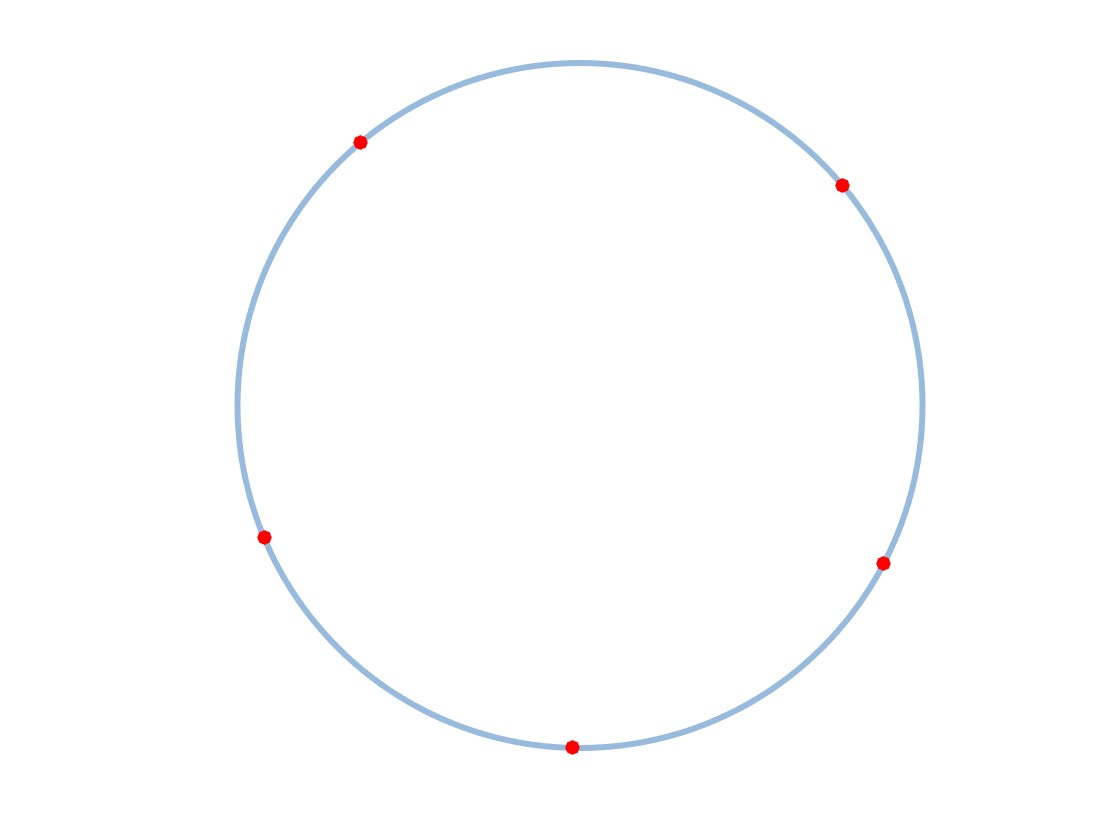
\includegraphics[width=\textwidth]{conf2_5_7.jpg}
        \caption{After $7$ iterations}
    \end{subfigure}
    \begin{subfigure}[b]{0.32\textwidth}
        \centering
        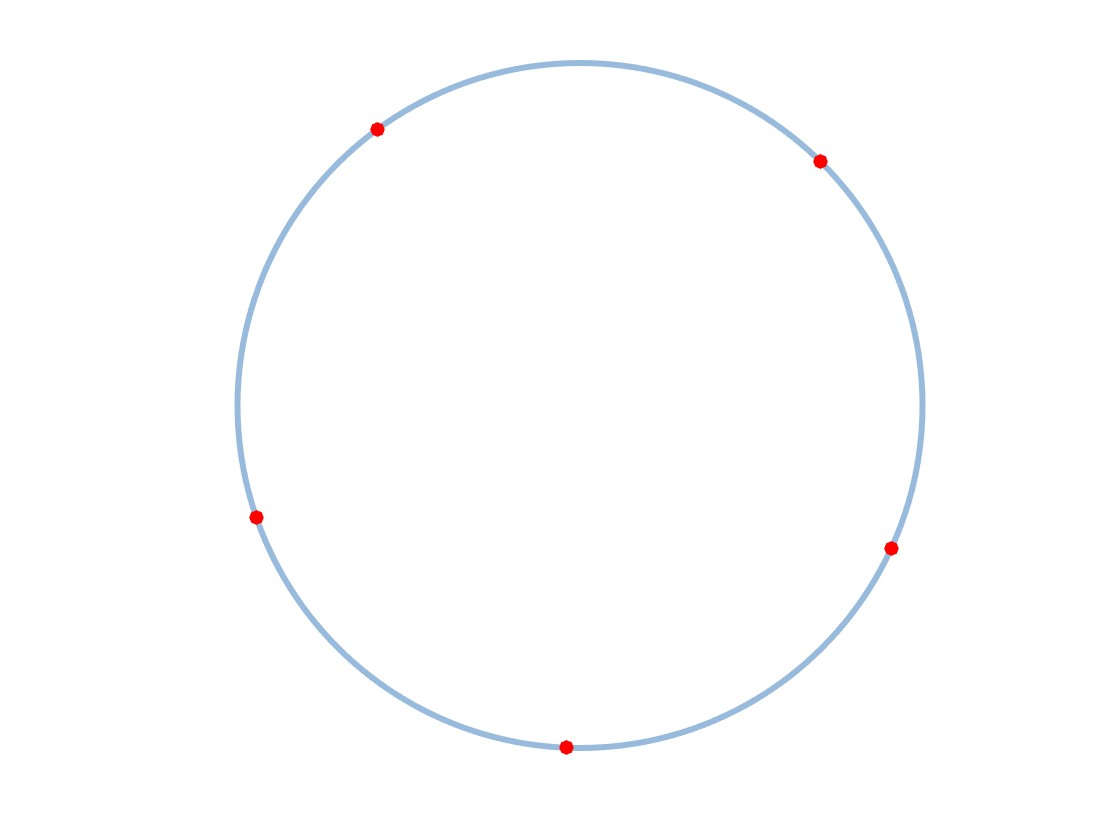
\includegraphics[width=\textwidth]{conf2_5_10.jpg}
        \caption{After $10$ iterations}
    \end{subfigure}
    \begin{subfigure}[b]{0.32\textwidth}
        \centering
        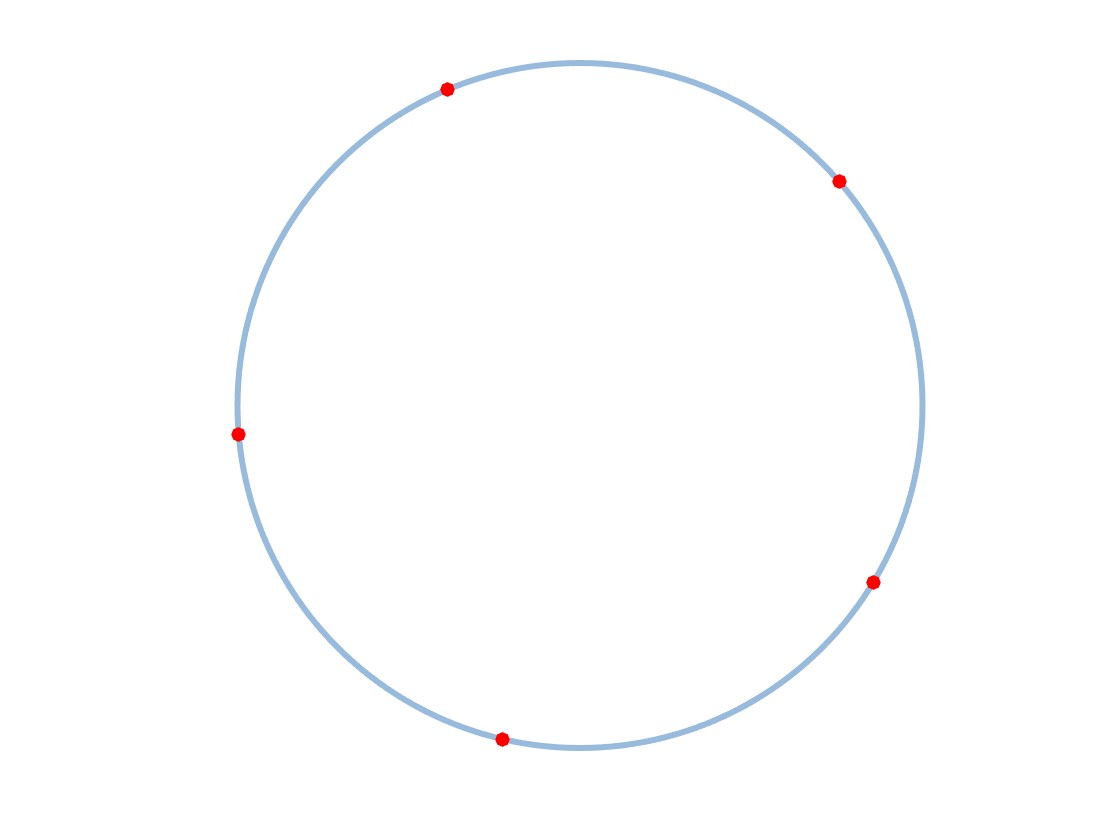
\includegraphics[width=\textwidth]{opt2_5.jpg}
        \caption{Best configuration obtained}
    \end{subfigure}

    \caption{Different configurations for $(2, 5)$}
    \label{fig:conf2_5}
\end{figure}



\begin{figure}[H]
    \centering
    \begin{subfigure}[b]{0.32\textwidth}
        \centering
        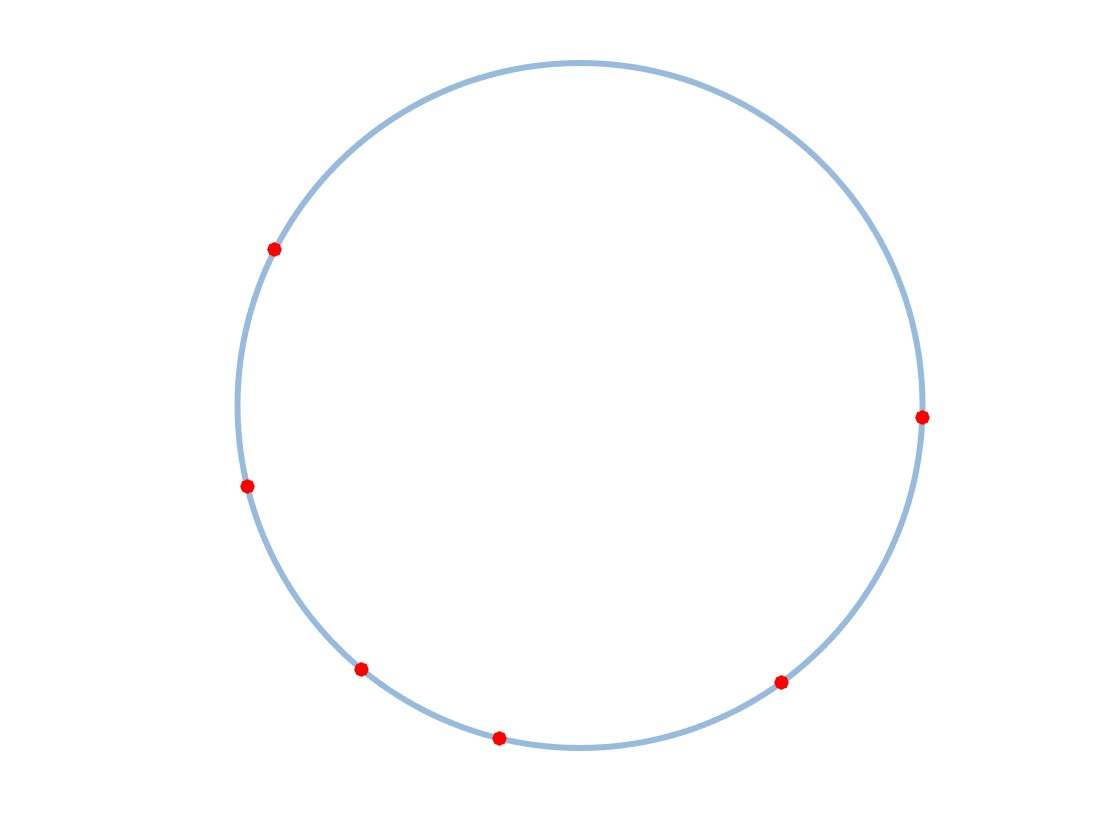
\includegraphics[width=\textwidth]{conf2_6_1.jpg}
        \caption{After $1$ iteration}
    \end{subfigure}
    \begin{subfigure}[b]{0.32\textwidth}
        \centering
        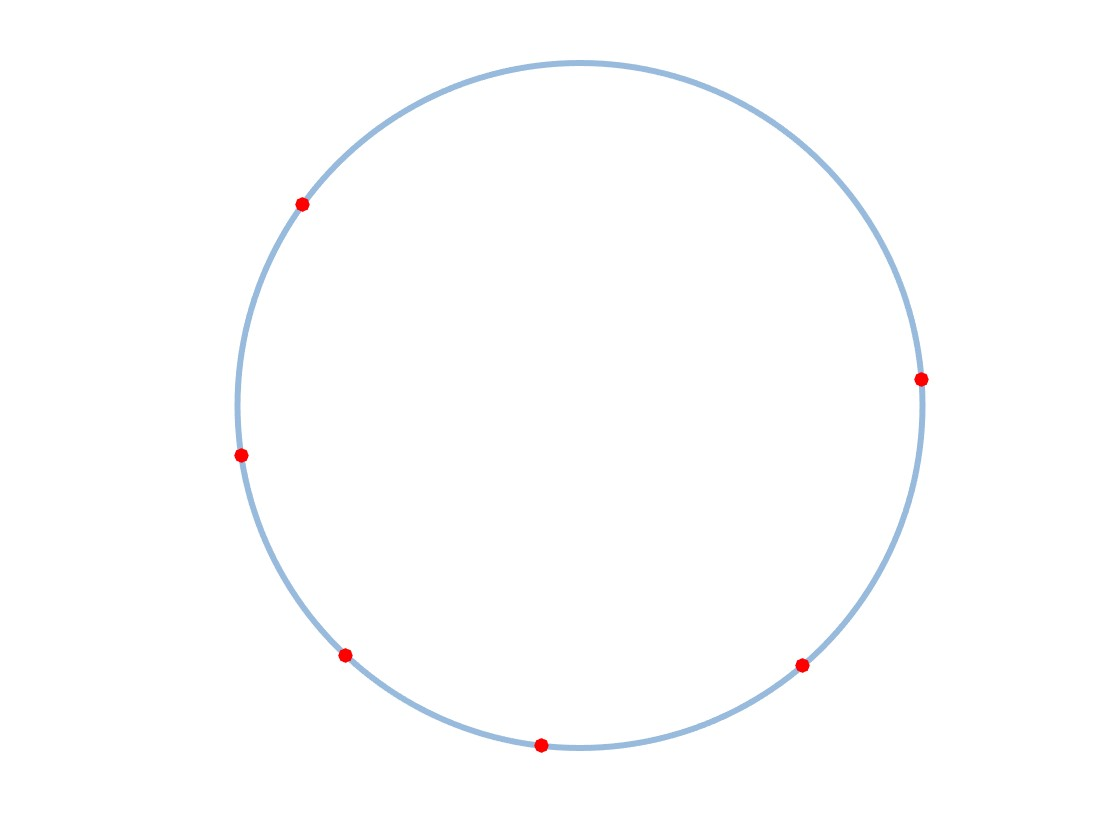
\includegraphics[width=\textwidth]{conf2_6_2.jpg}
        \caption{After $2$ iterations}
    \end{subfigure}
    \begin{subfigure}[b]{0.32\textwidth}
        \centering
        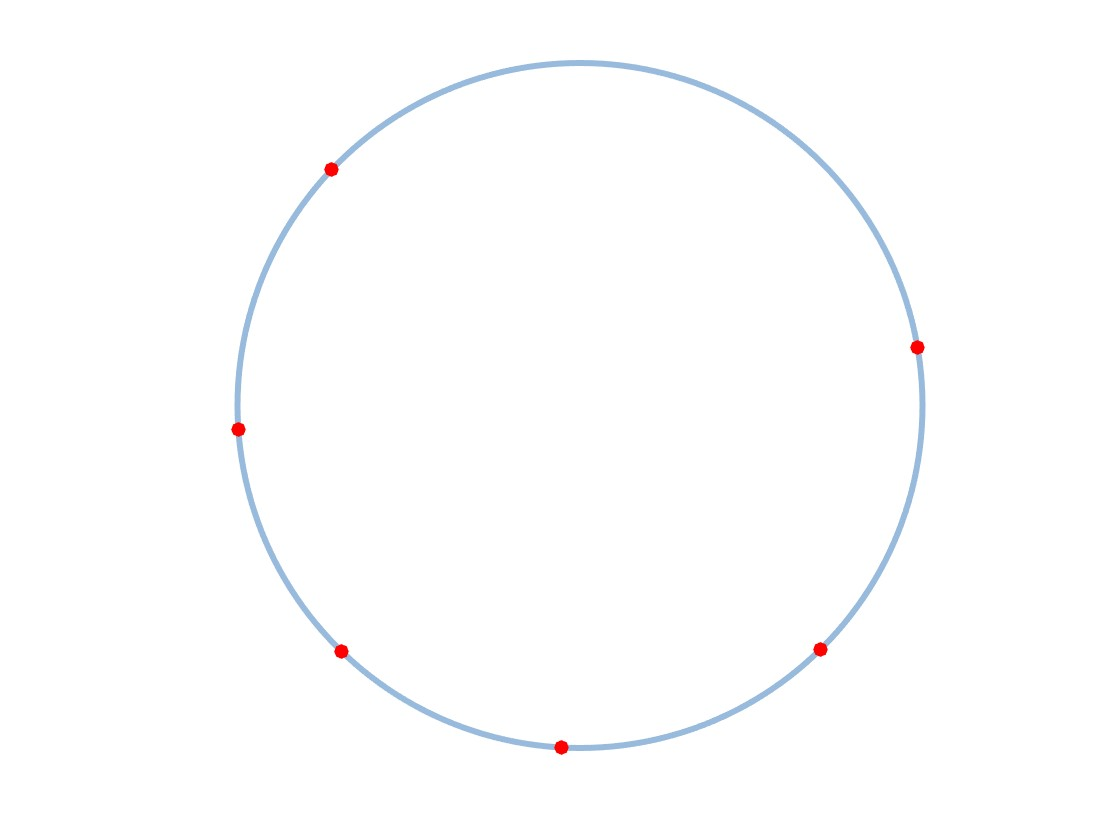
\includegraphics[width=\textwidth]{conf2_6_3.jpg}
        \caption{After $3$ iterations}
    \end{subfigure}

    \begin{subfigure}[b]{0.32\textwidth}
        \centering
        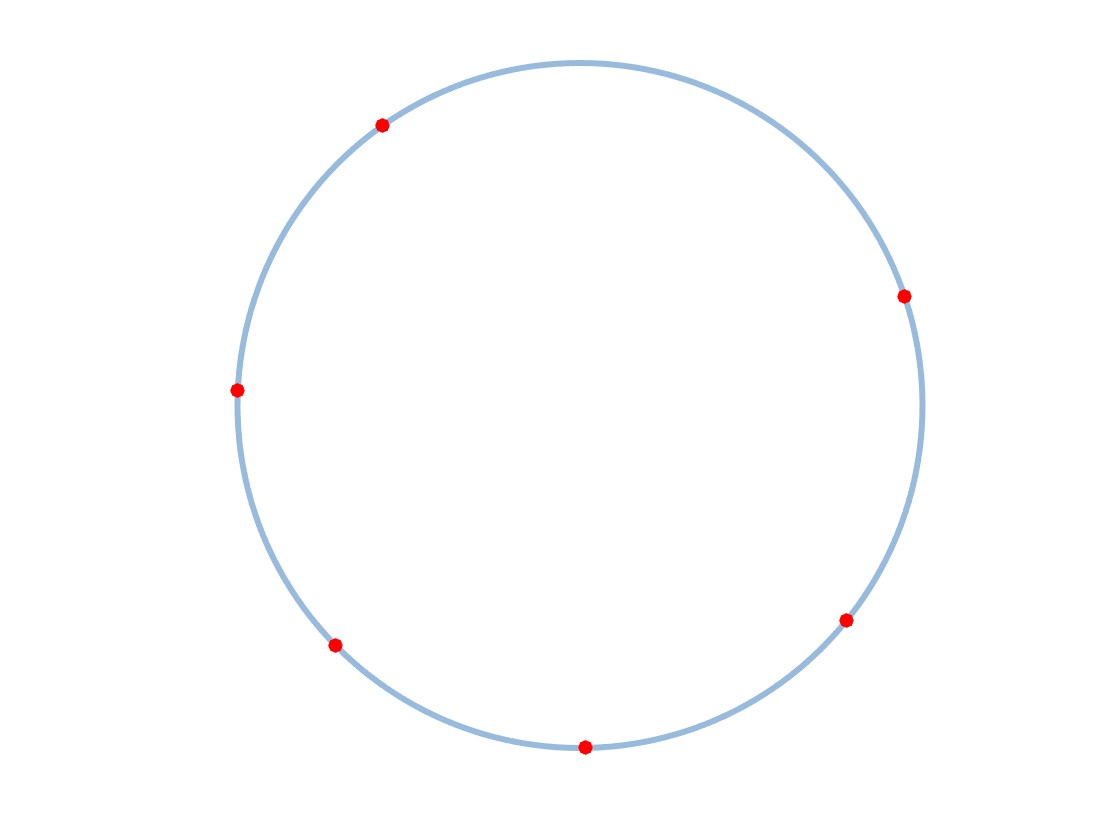
\includegraphics[width=\textwidth]{conf2_6_5.jpg}
        \caption{After $5$ iterations}
    \end{subfigure}
    \begin{subfigure}[b]{0.32\textwidth}
        \centering
        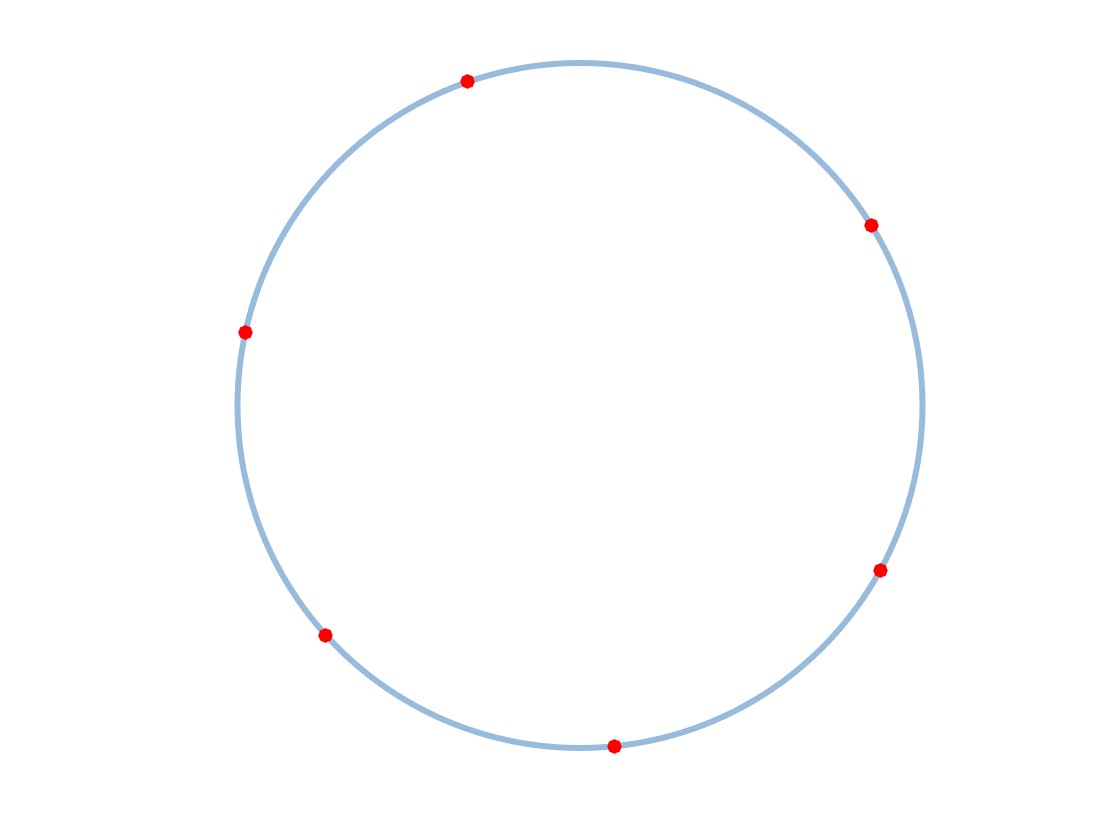
\includegraphics[width=\textwidth]{conf2_6_10.jpg}
        \caption{After $10$ iterations}
    \end{subfigure}
    \begin{subfigure}[b]{0.32\textwidth}
        \centering
        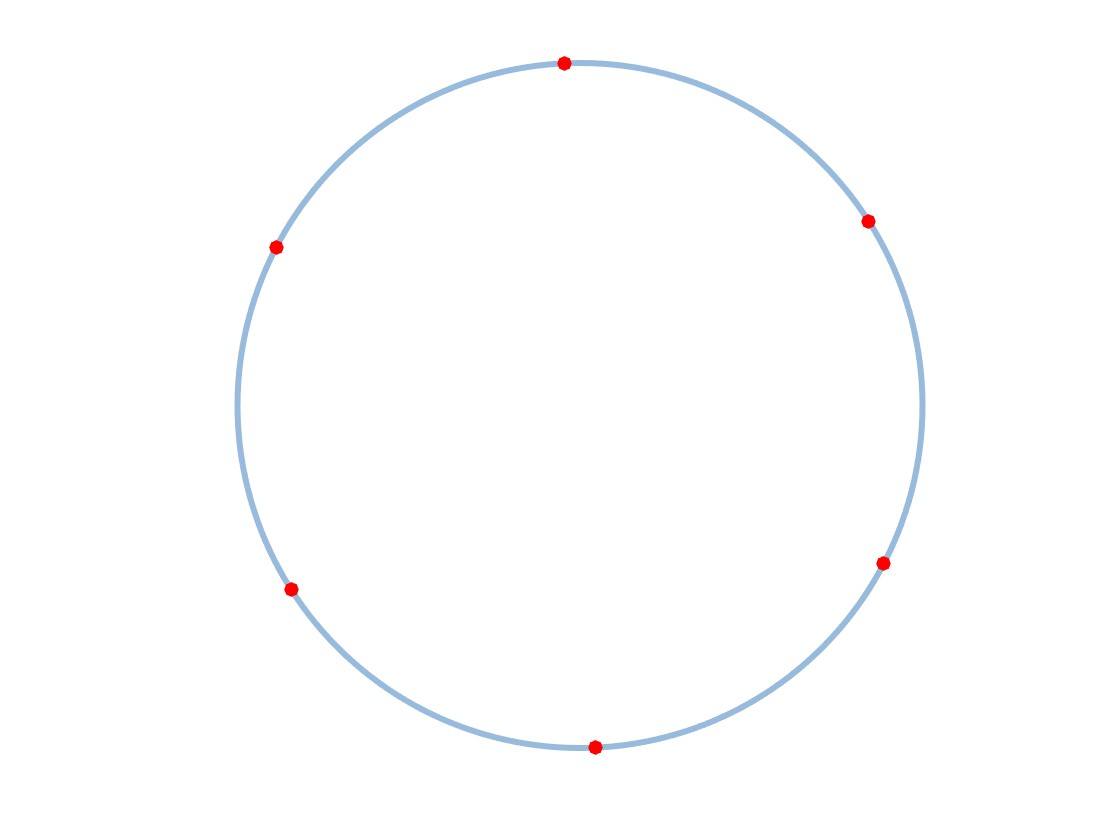
\includegraphics[width=\textwidth]{opt2_6.jpg}
        \caption{Best configuration obtained}
    \end{subfigure}

    \caption{Different configurations for $(2, 6)$}
    \label{fig:conf2_6}
\end{figure}

Figures \ref{fig:conf3_2}, \ref{fig:conf3_3}, \ref{fig:conf3_4}, \ref{fig:conf3_5}, \ref{fig:conf3_6}, \ref{fig:conf3_12} and \ref{fig:conf3_16} show the different configurations for different numbers of iterations for $d=3$ and $n\in\{2, 3, 4, 5, 6, 12, 16\}$. The observations are similar to the case $d=2$. As the number of iterations increases, the points move further apart until they are well spread on the surface of the sphere. Again, for smaller values of $n$ the best configuration is quickly attained, whereas for larger values, e.g. $n=12, 16$, more steps are needed.

\begin{figure}[H]
    \centering
    \begin{subfigure}[b]{0.32\textwidth}
        \centering
        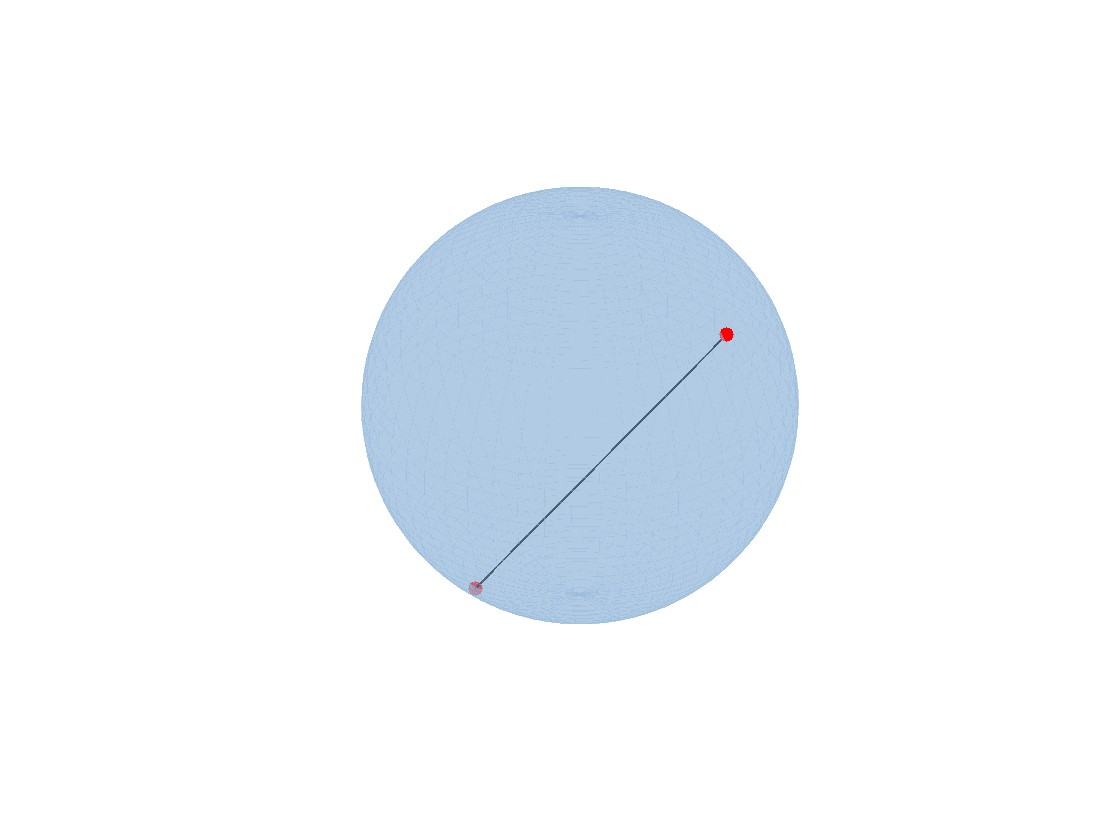
\includegraphics[width=\textwidth]{conf3_2_1.jpg}
        \caption{After $1$ iteration}
    \end{subfigure}
    \begin{subfigure}[b]{0.32\textwidth}
        \centering
        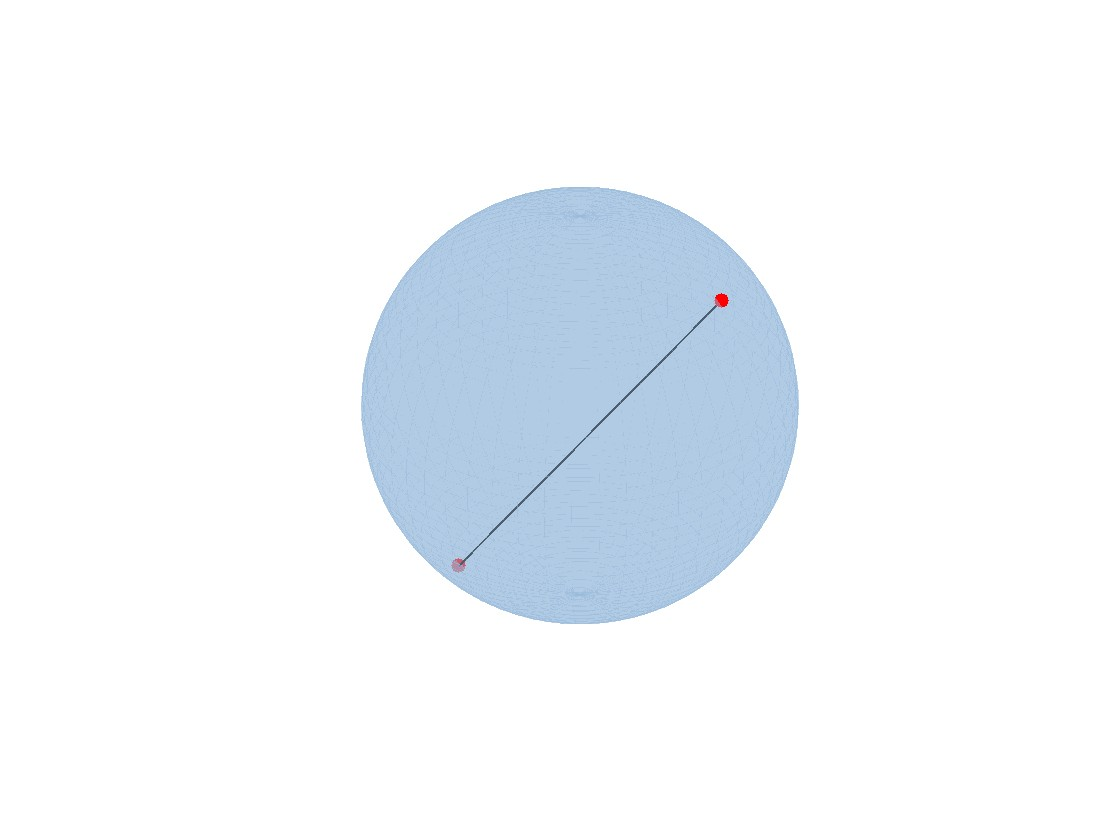
\includegraphics[width=\textwidth]{conf3_2_2.jpg}
        \caption{After $2$ iterations}
    \end{subfigure}

    \begin{subfigure}[b]{0.32\textwidth}
        \centering
        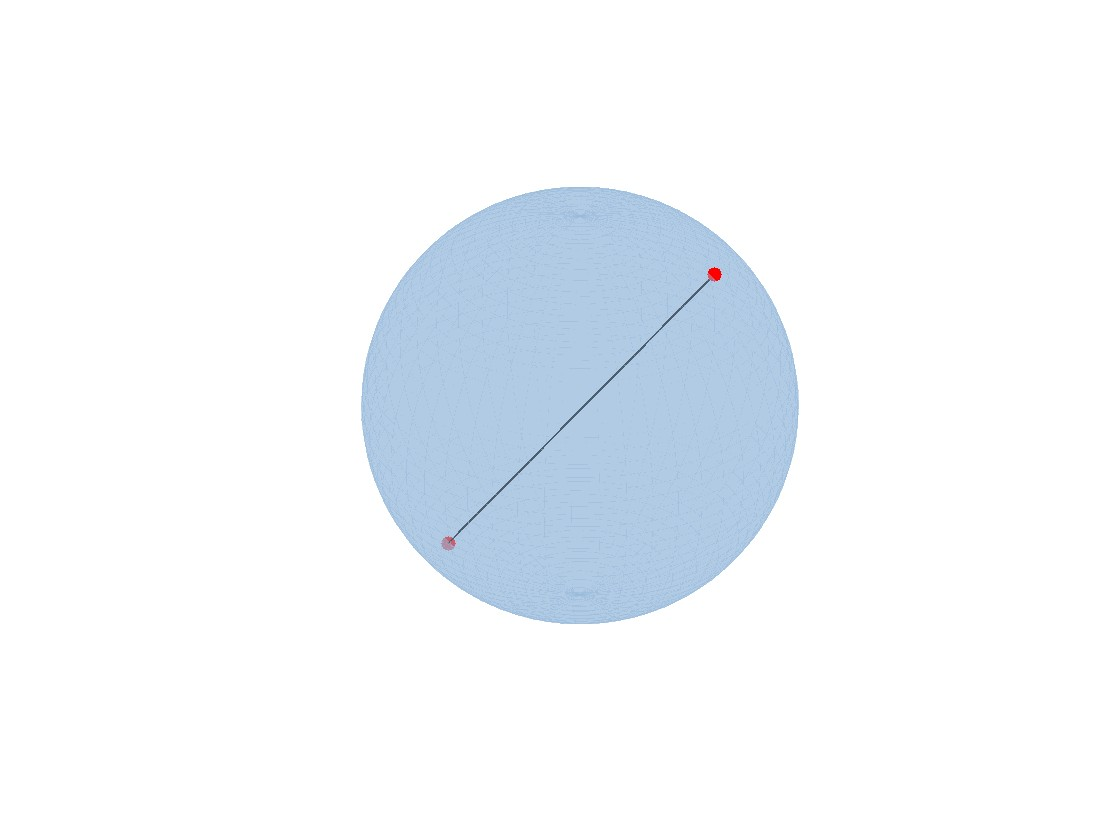
\includegraphics[width=\textwidth]{conf3_2_5.jpg}
        \caption{After $5$ iterations}
    \end{subfigure}
    \begin{subfigure}[b]{0.32\textwidth}
        \centering
        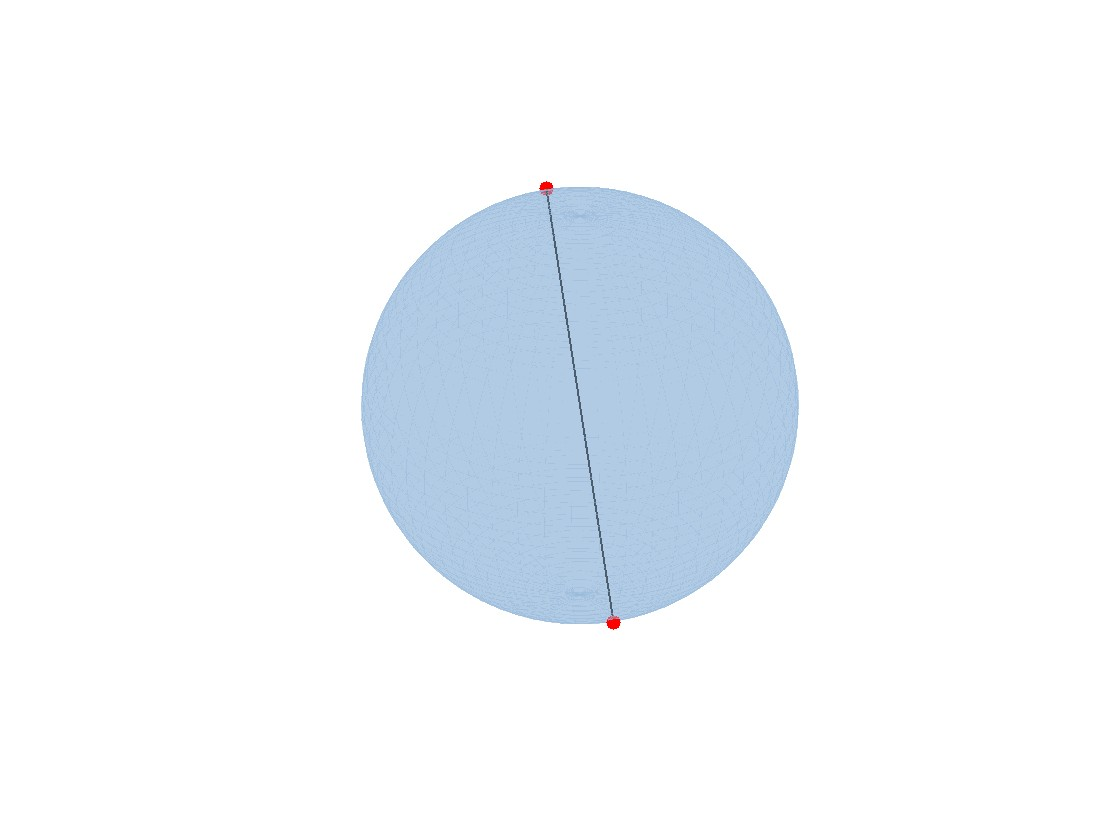
\includegraphics[width=\textwidth]{opt3_2.jpg}
        \caption{Optimal configuration obtained}
    \end{subfigure}

    \caption{Different configurations for $(3, 2)$}
    \label{fig:conf3_2}
\end{figure}



\begin{figure}[H]
    \centering
    \begin{subfigure}[b]{0.32\textwidth}
        \centering
        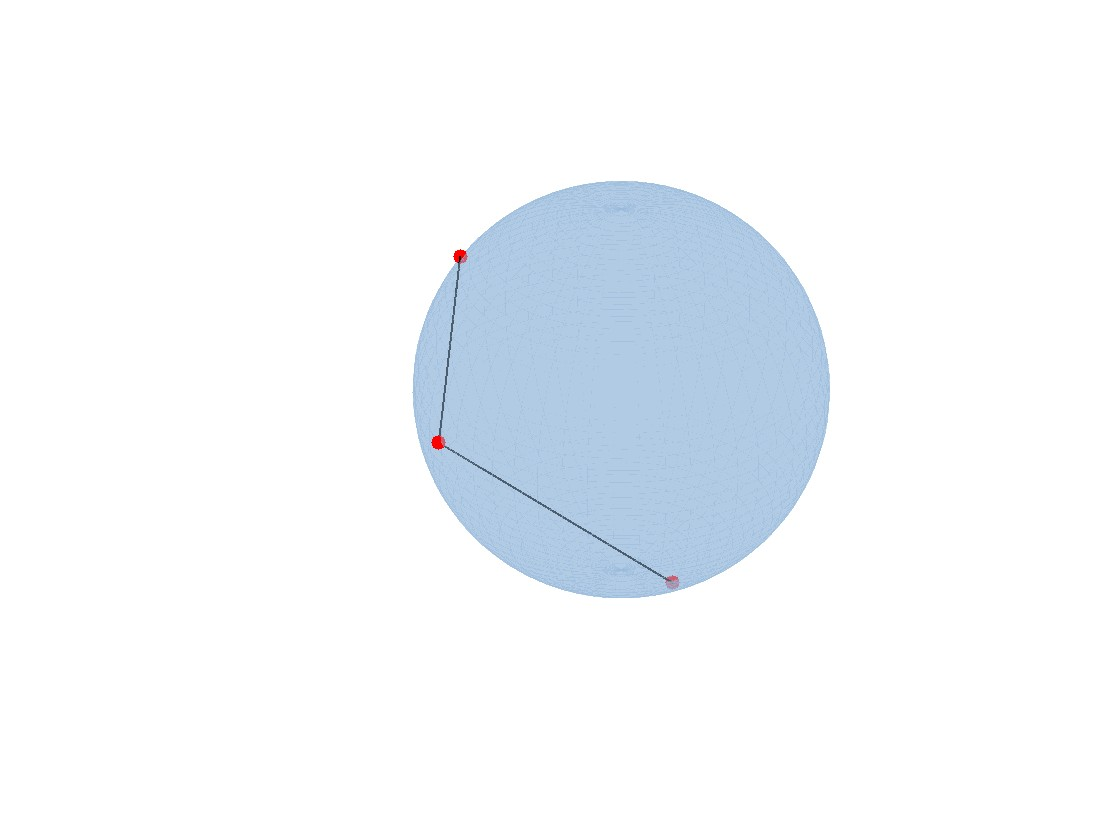
\includegraphics[width=\textwidth]{conf3_3_1.jpg}
        \caption{After $1$ iteration}
    \end{subfigure}
    \begin{subfigure}[b]{0.32\textwidth}
        \centering
        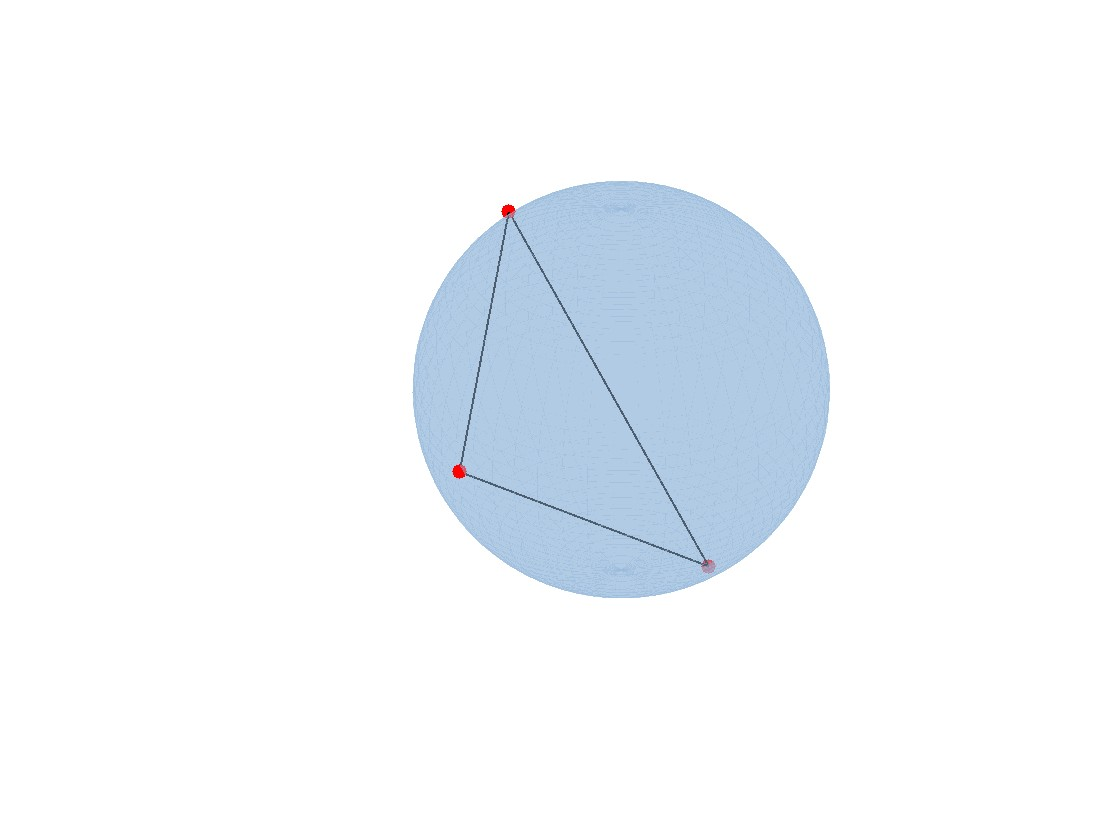
\includegraphics[width=\textwidth]{conf3_3_2.jpg}
        \caption{After $2$ iterations}
    \end{subfigure}
    \begin{subfigure}[b]{0.32\textwidth}
        \centering
        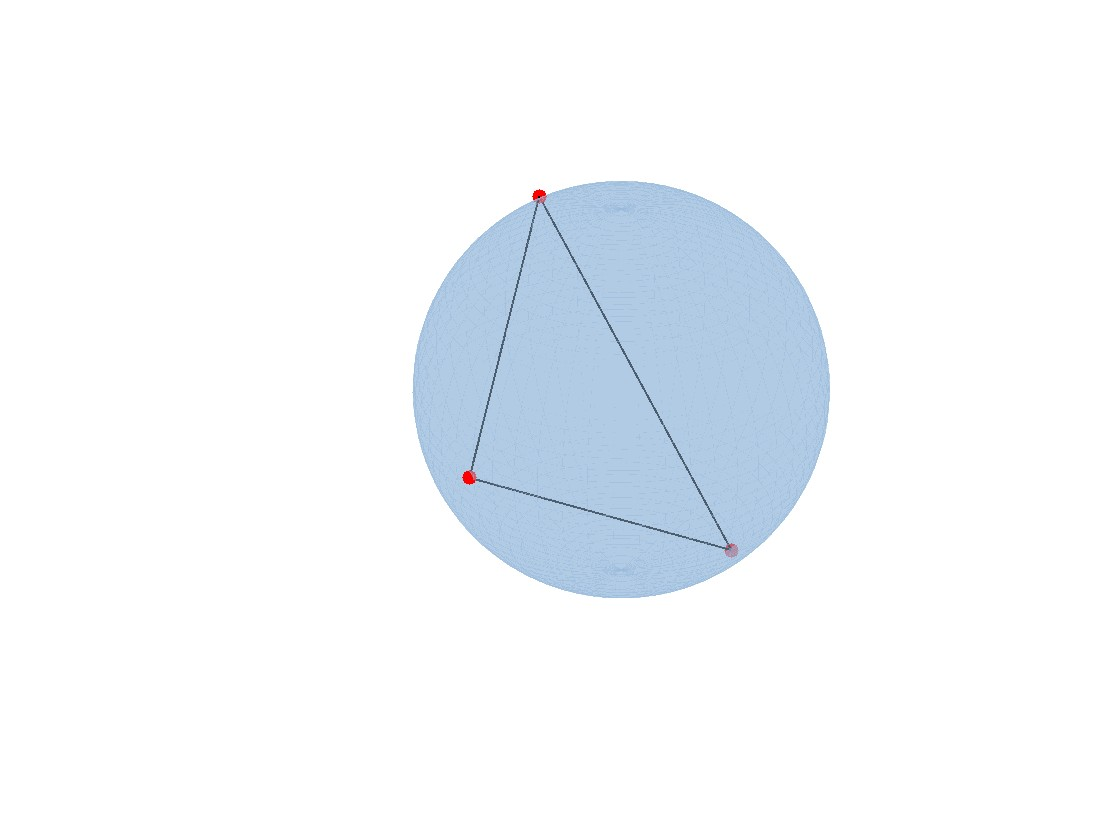
\includegraphics[width=\textwidth]{conf3_3_3.jpg}
        \caption{After $3$ iterations}
    \end{subfigure}

    \begin{subfigure}[b]{0.32\textwidth}
        \centering
        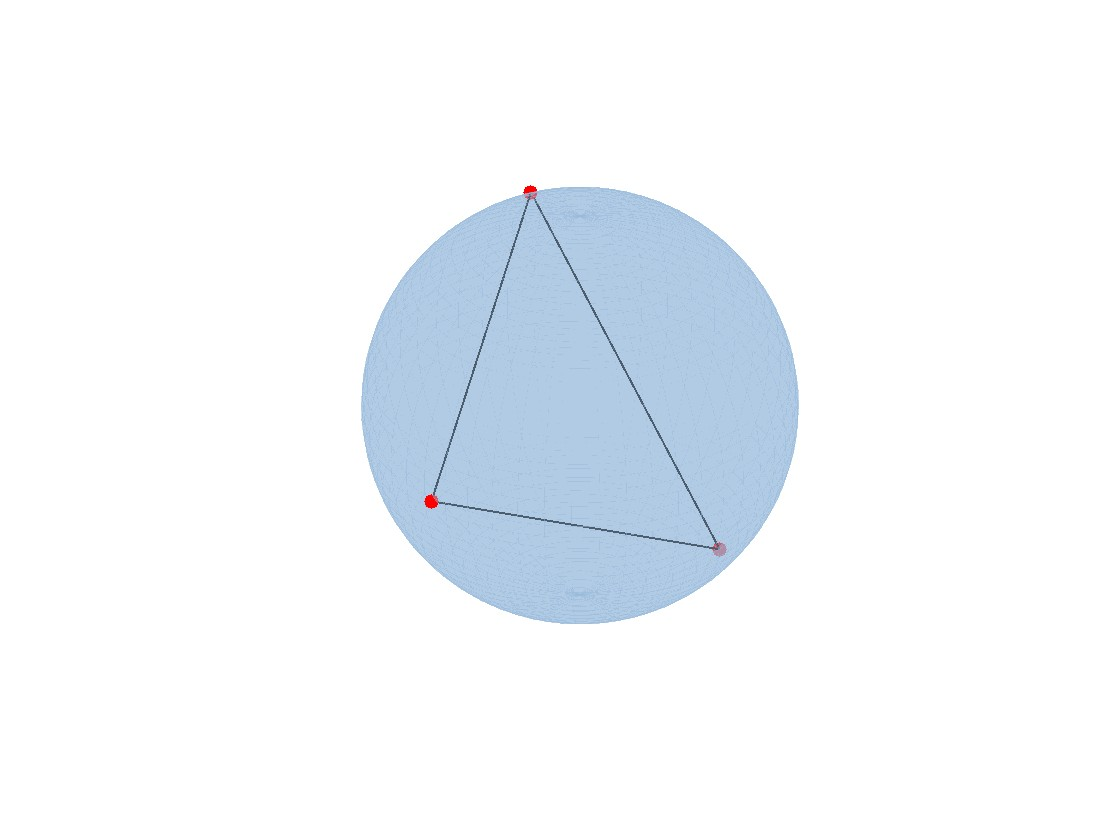
\includegraphics[width=\textwidth]{conf3_3_5.jpg}
        \caption{After $5$ iterations}
    \end{subfigure}
    \begin{subfigure}[b]{0.32\textwidth}
        \centering
        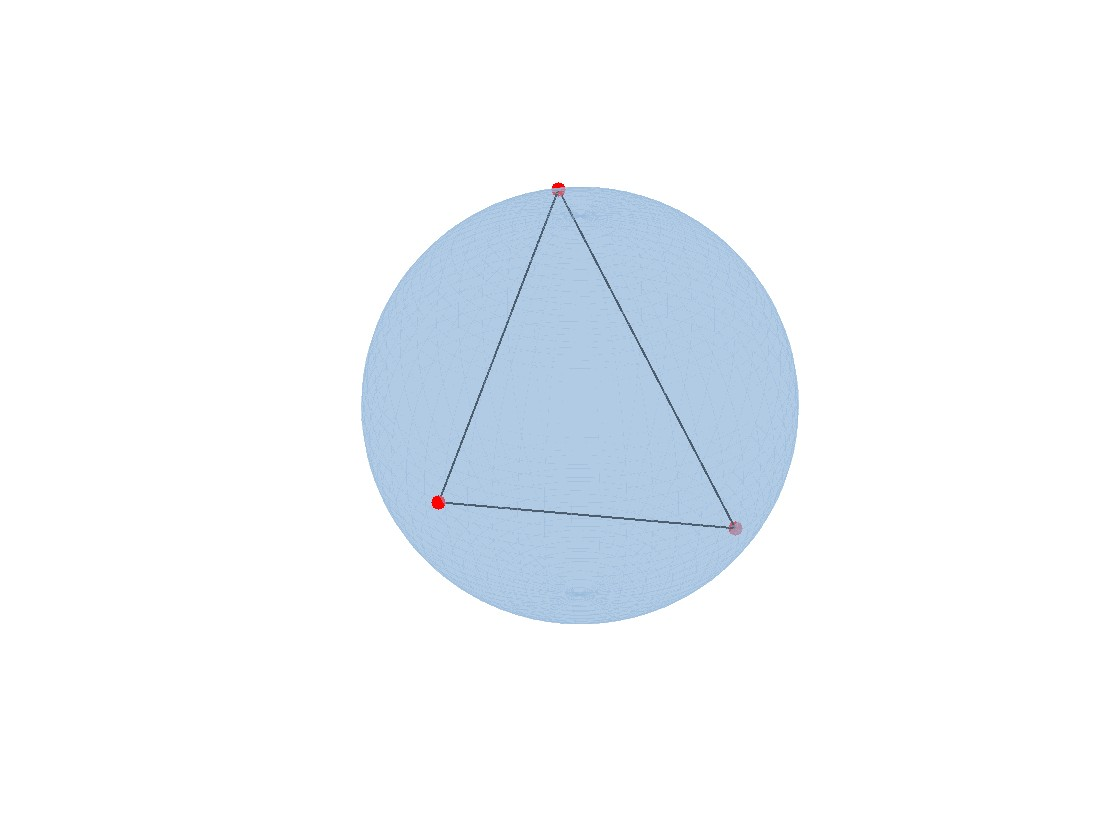
\includegraphics[width=\textwidth]{conf3_3_10.jpg}
        \caption{After $10$ iterations}
    \end{subfigure}
    \begin{subfigure}[b]{0.32\textwidth}
        \centering
        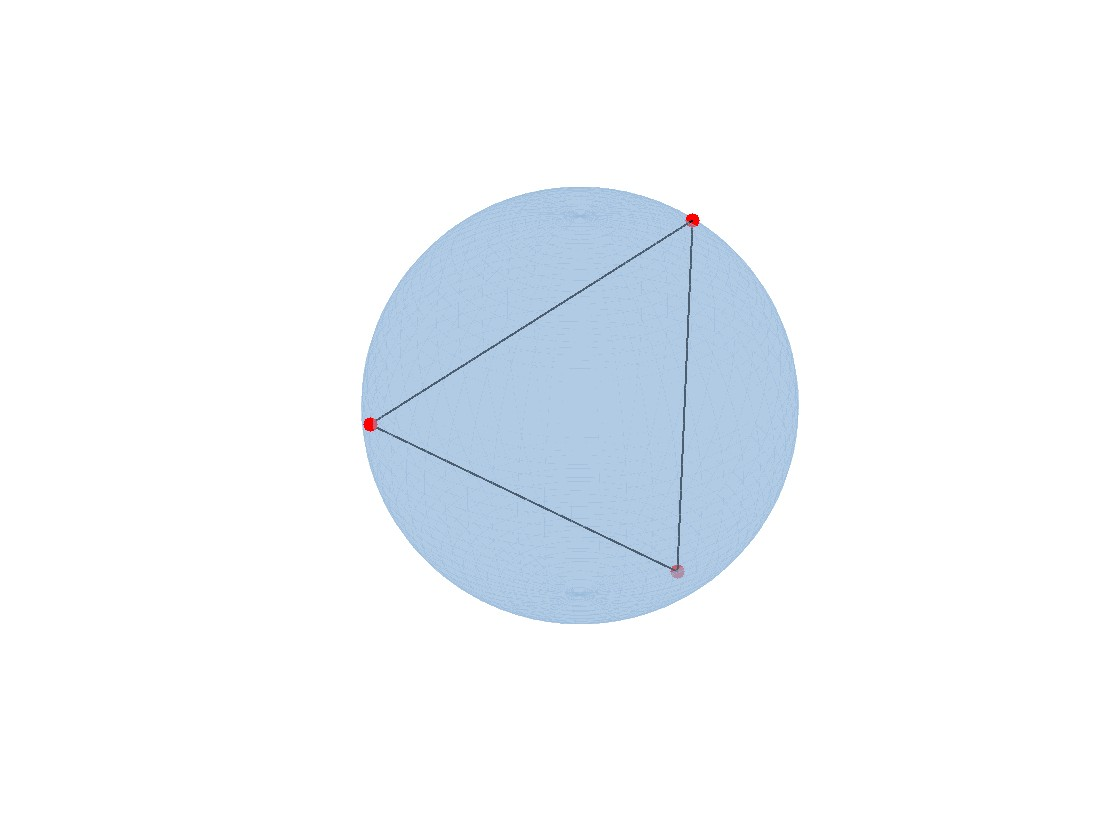
\includegraphics[width=\textwidth]{opt3_3.jpg}
        \caption{Optimal configuration obtained}
    \end{subfigure}

    \caption{Different configurations for $(3, 3)$}
    \label{fig:conf3_3}
\end{figure}



\begin{figure}[H]
    \centering
    \begin{subfigure}[b]{0.32\textwidth}
        \centering
        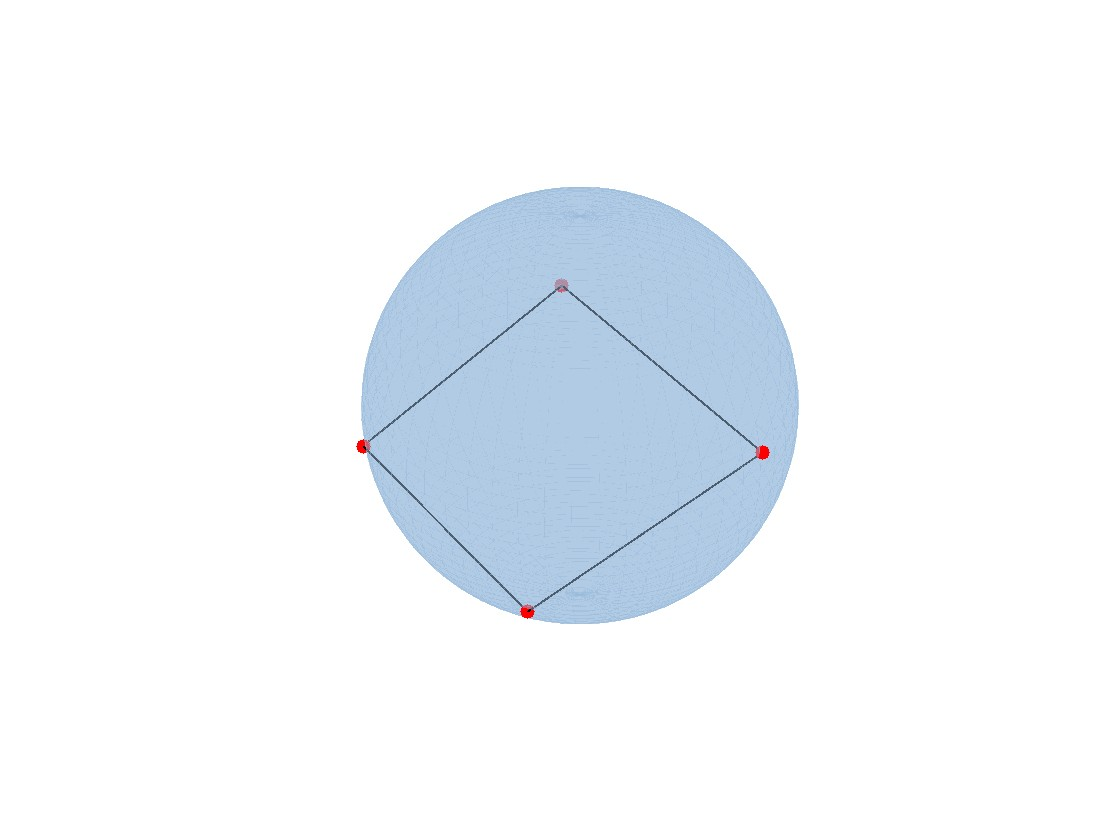
\includegraphics[width=\textwidth]{conf3_4_1.jpg}
        \caption{After $1$ iteration}
    \end{subfigure}
    \begin{subfigure}[b]{0.32\textwidth}
        \centering
        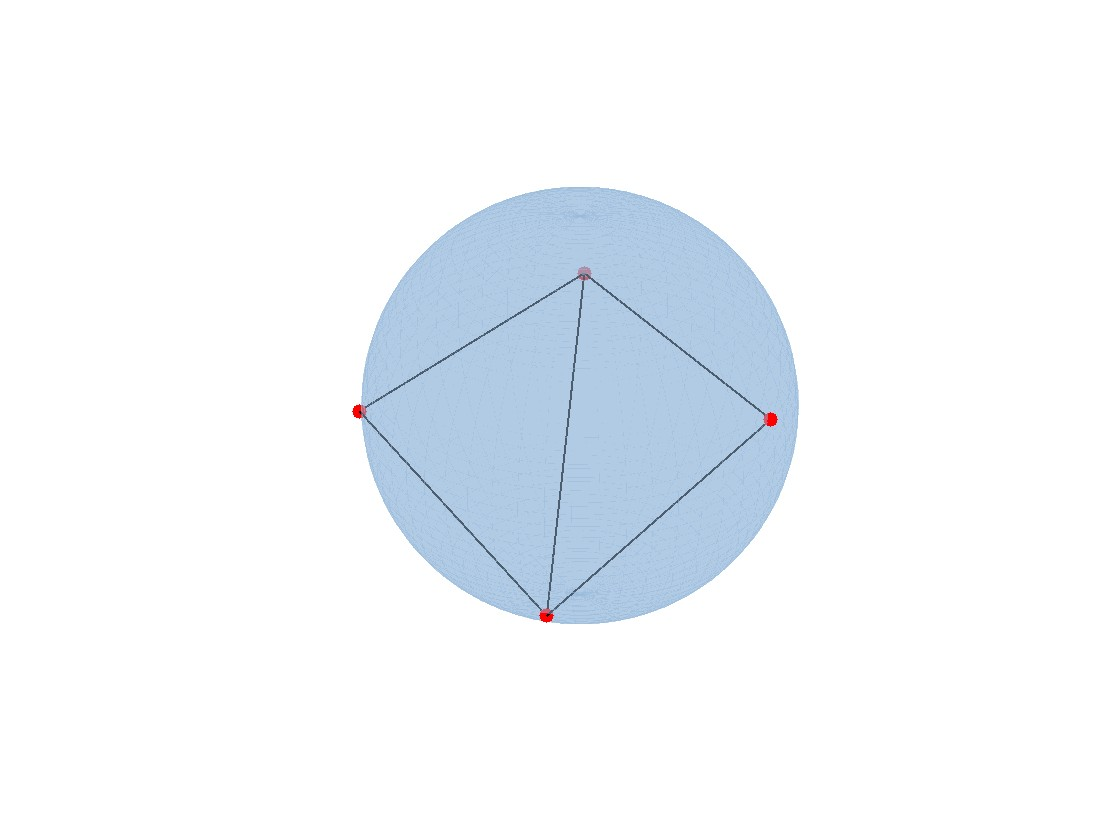
\includegraphics[width=\textwidth]{conf3_4_3.jpg}
        \caption{After $3$ iterations}
    \end{subfigure}
    \begin{subfigure}[b]{0.32\textwidth}
        \centering
        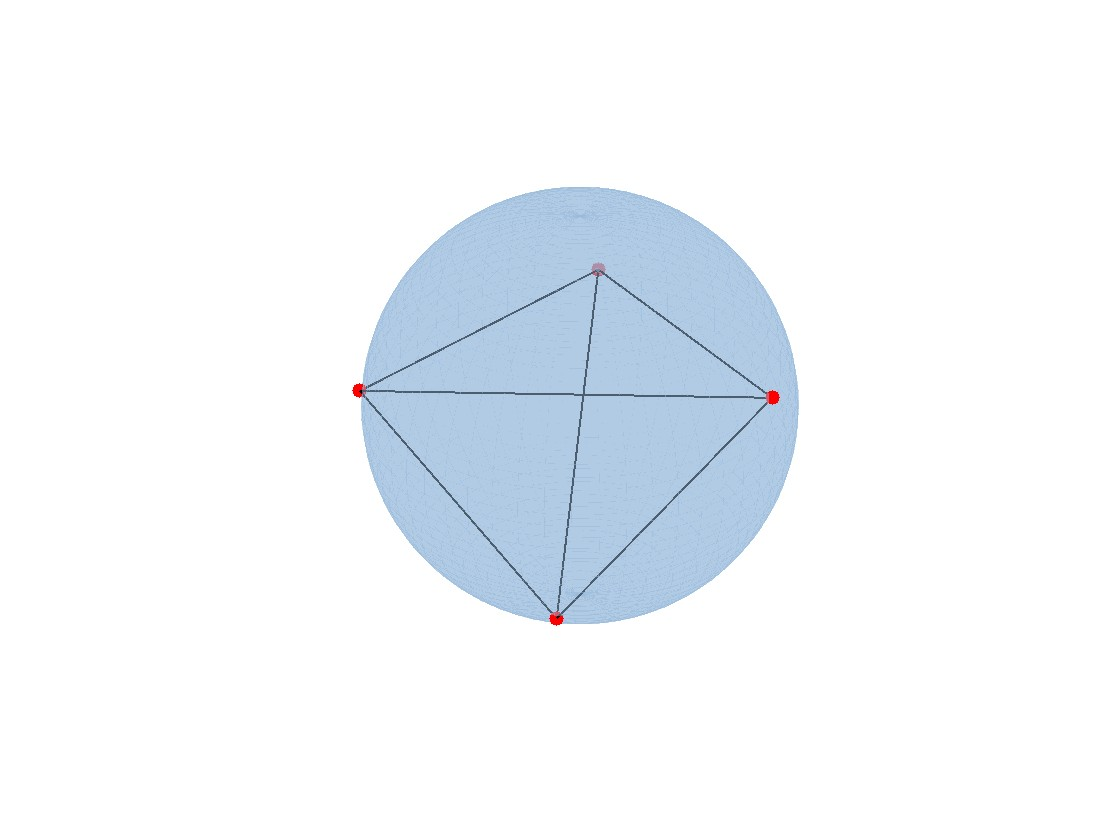
\includegraphics[width=\textwidth]{conf3_4_5.jpg}
        \caption{After $5$ iterations}
    \end{subfigure}

    \begin{subfigure}[b]{0.32\textwidth}
        \centering
        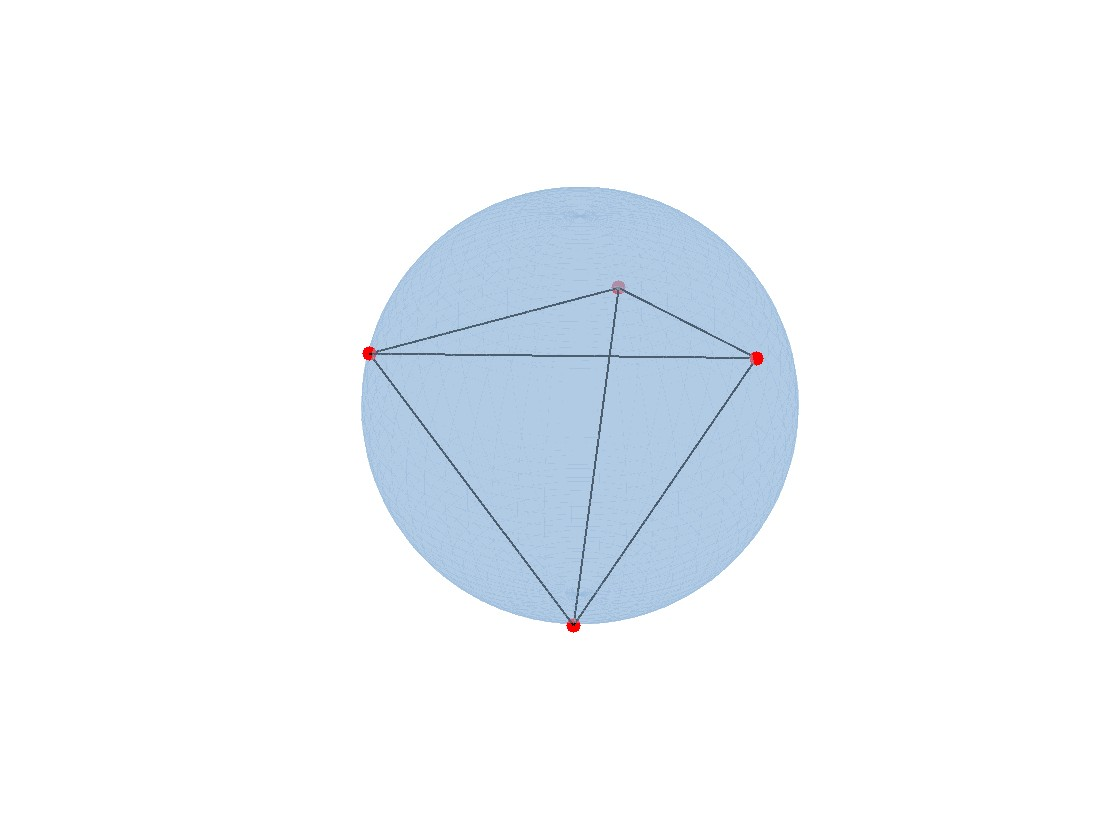
\includegraphics[width=\textwidth]{conf3_4_15.jpg}
        \caption{After $15$ iterations}
    \end{subfigure}
    \begin{subfigure}[b]{0.32\textwidth}
        \centering
        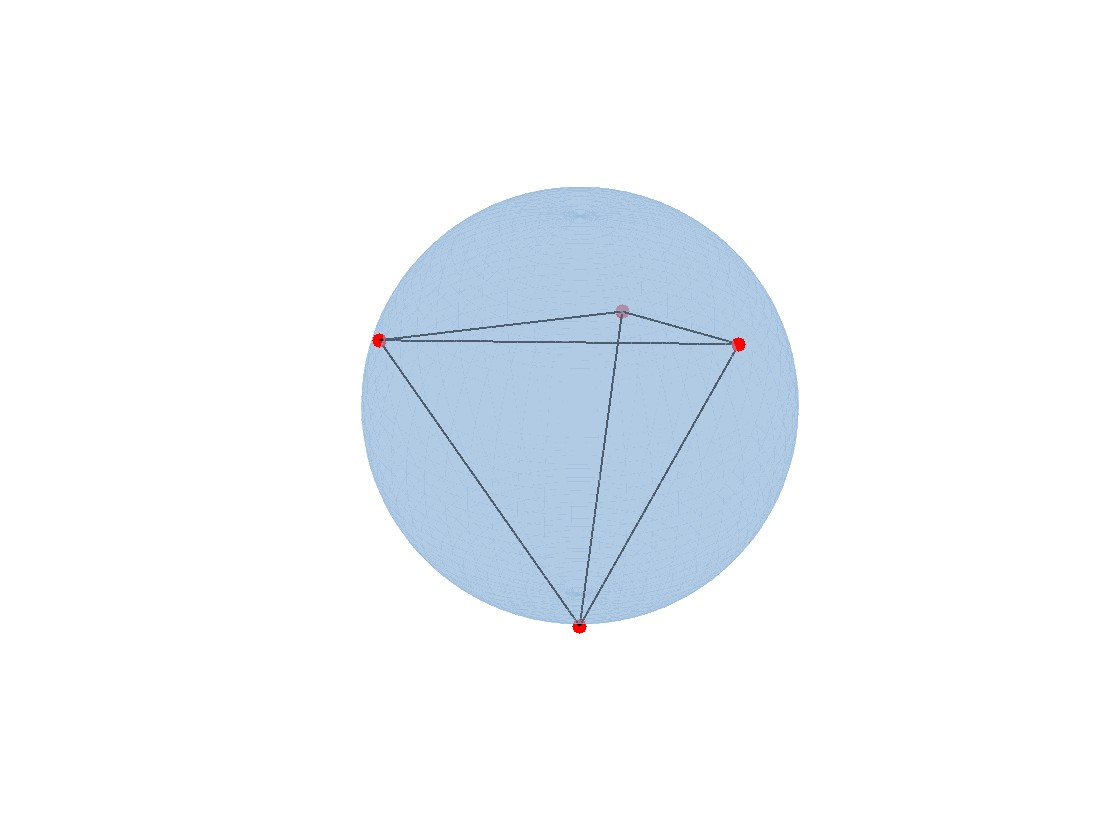
\includegraphics[width=\textwidth]{conf3_4_30.jpg}
        \caption{After $30$ iterations}
    \end{subfigure}
    \begin{subfigure}[b]{0.32\textwidth}
        \centering
        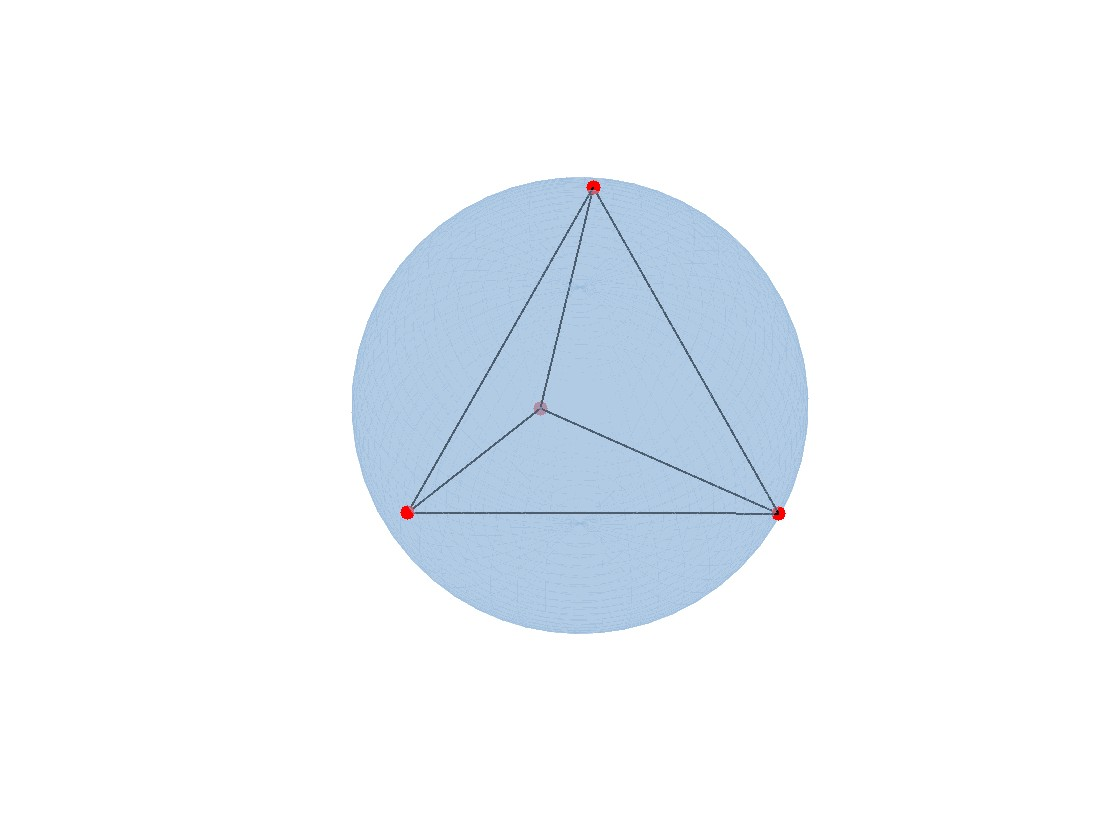
\includegraphics[width=\textwidth]{opt3_4.jpg}
        \caption{Best configuration obtained}
    \end{subfigure}

    \caption{Different configurations for $(3, 4)$}
    \label{fig:conf3_4}
\end{figure}


\begin{figure}[H]
    \centering
    \begin{subfigure}[b]{0.32\textwidth}
        \centering
        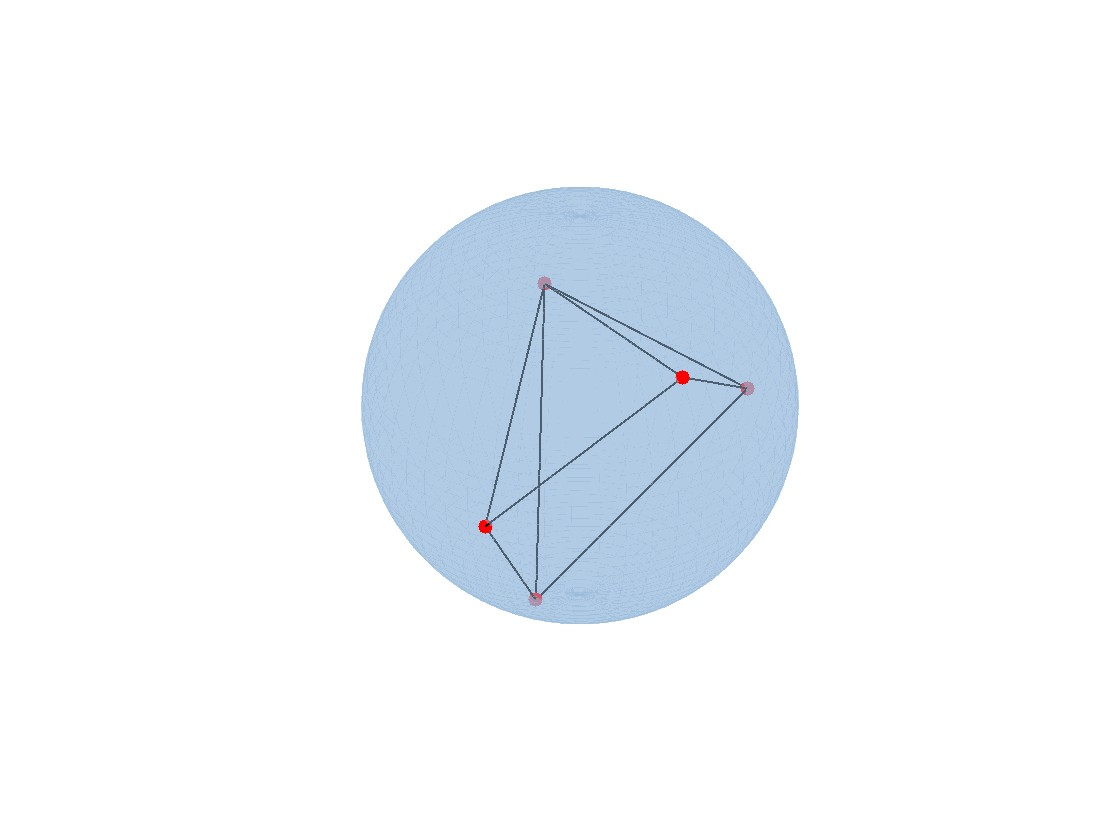
\includegraphics[width=\textwidth]{conf3_5_1.jpg}
        \caption{After $1$ iteration}
    \end{subfigure}
    \begin{subfigure}[b]{0.32\textwidth}
        \centering
        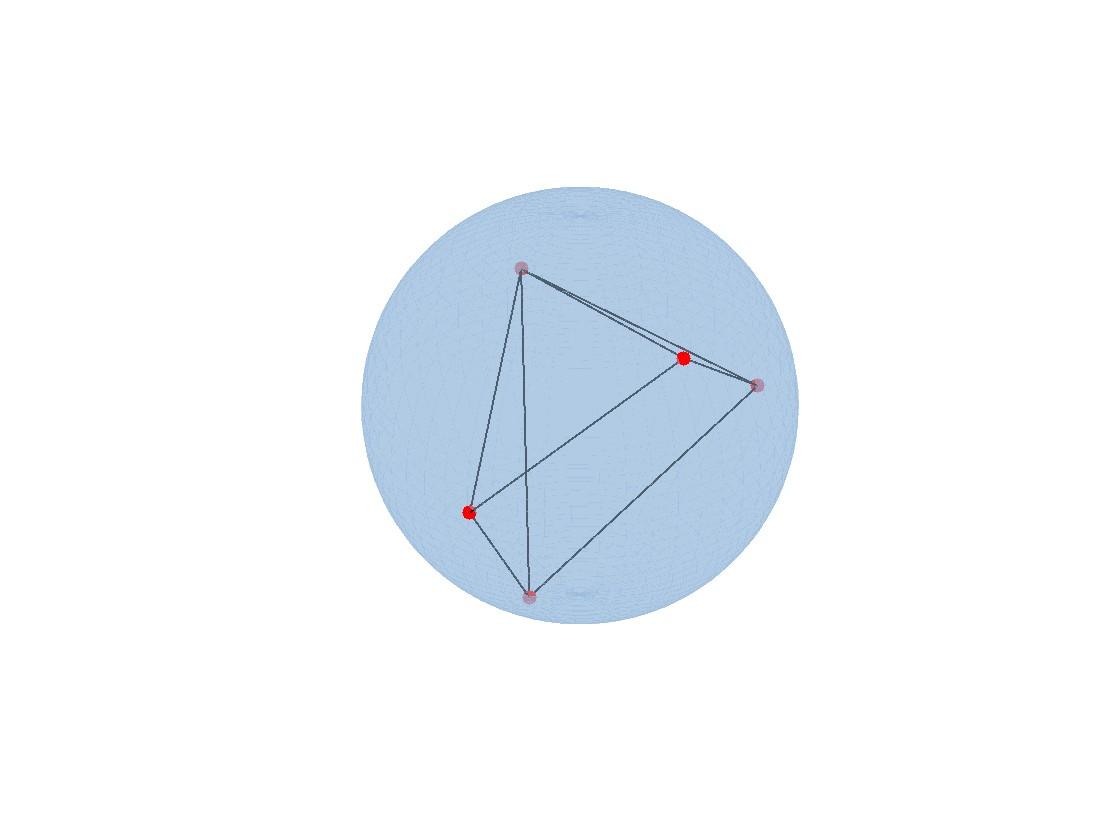
\includegraphics[width=\textwidth]{conf3_5_3.jpg}
        \caption{After $3$ iterations}
    \end{subfigure}
    \begin{subfigure}[b]{0.32\textwidth}
        \centering
        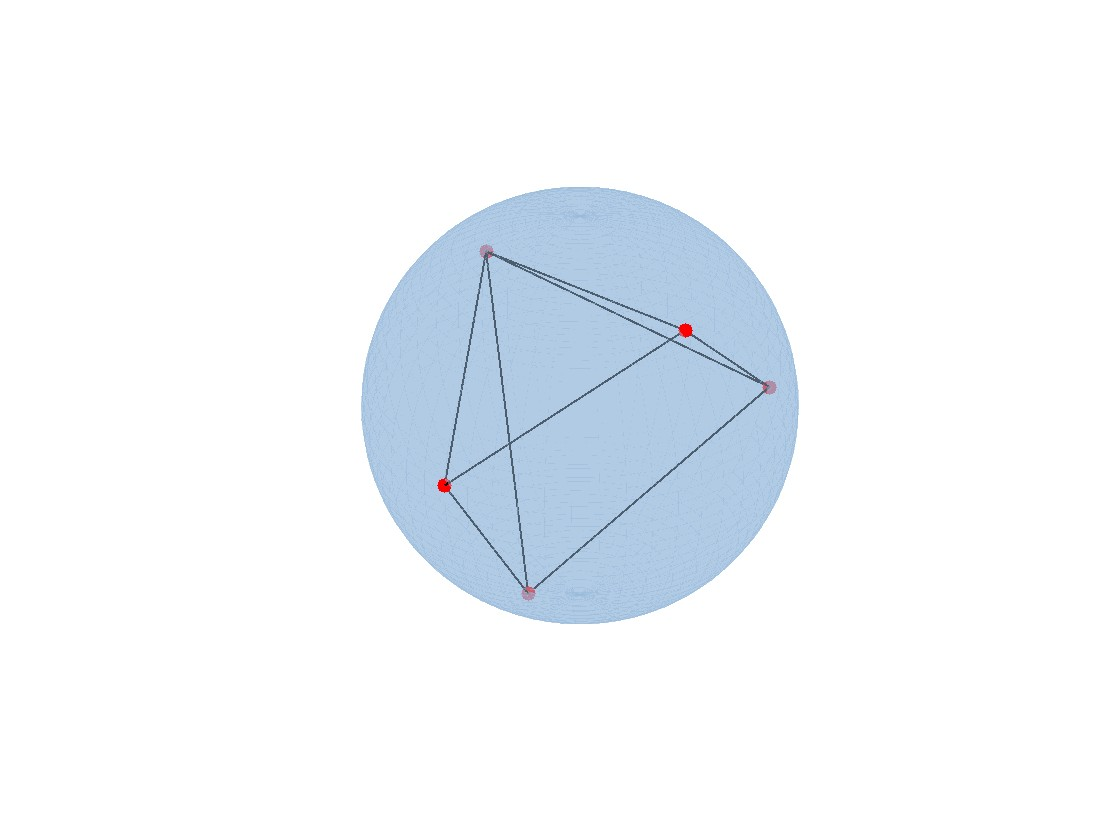
\includegraphics[width=\textwidth]{conf3_5_10.jpg}
        \caption{After $10$ iterations}
    \end{subfigure}

    \begin{subfigure}[b]{0.32\textwidth}
        \centering
        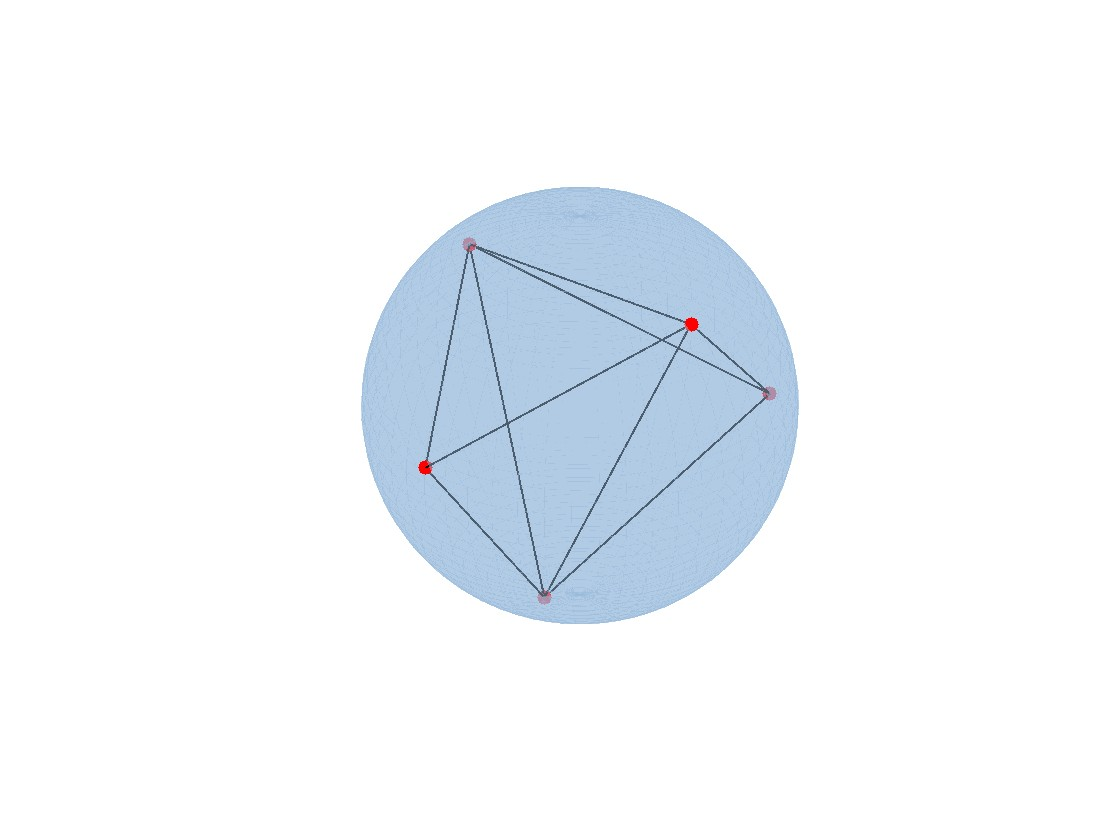
\includegraphics[width=\textwidth]{conf3_5_50.jpg}
        \caption{After $50$ iterations}
    \end{subfigure}
    \begin{subfigure}[b]{0.32\textwidth}
        \centering
        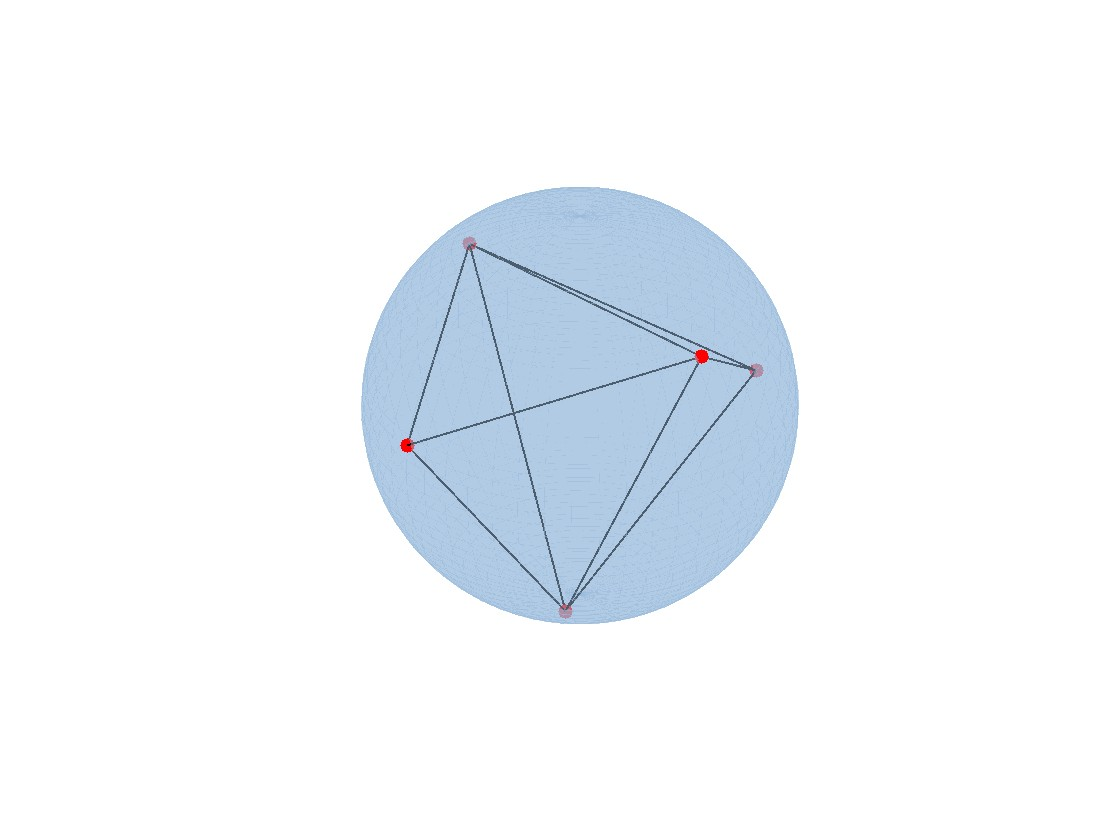
\includegraphics[width=\textwidth]{conf3_5_200.jpg}
        \caption{After $200$ iterations}
    \end{subfigure}
    \begin{subfigure}[b]{0.32\textwidth}
        \centering
        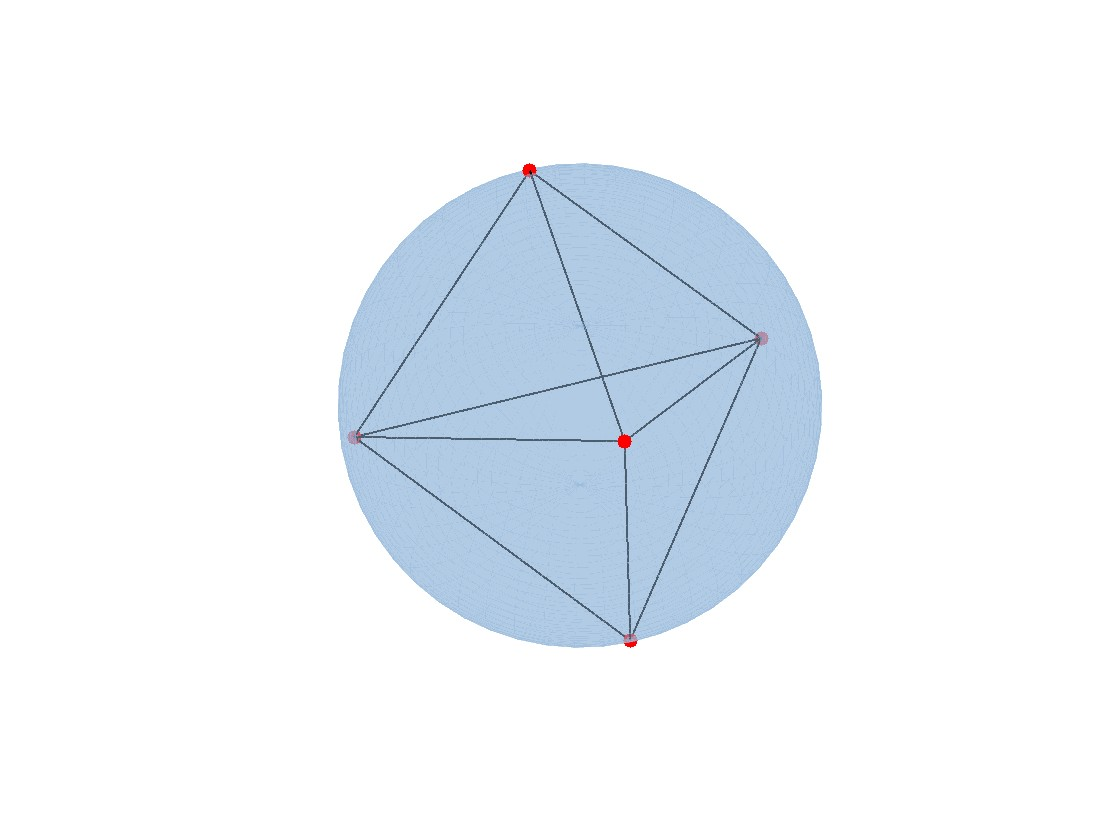
\includegraphics[width=\textwidth]{opt3_5.jpg}
        \caption{Best configuration obtained}
    \end{subfigure}

    \caption{Different configurations for $(3, 5)$}
    \label{fig:conf3_5}
\end{figure}



\begin{figure}[H]
    \centering
    % Première ligne : 3 images
    \begin{subfigure}[b]{0.32\textwidth}
        \centering
        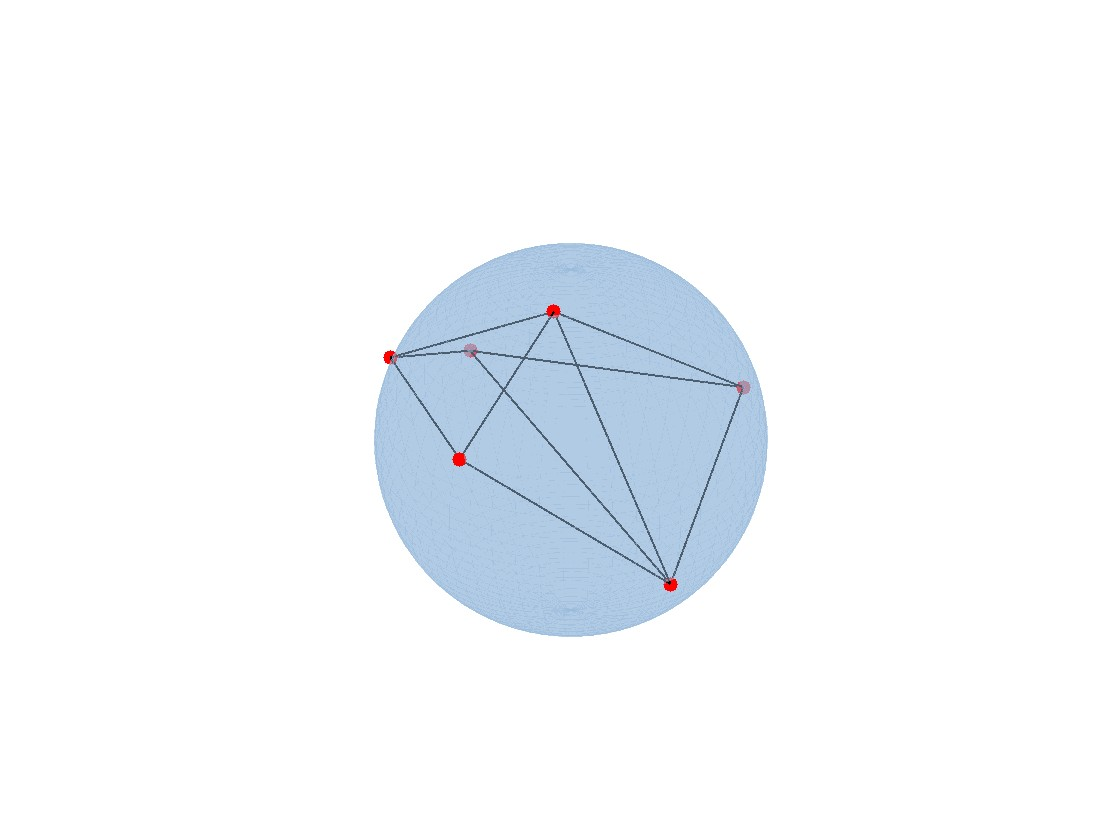
\includegraphics[width=\textwidth]{conf3_6_1.jpg}
        \caption{After $1$ iteration}
    \end{subfigure}
    \begin{subfigure}[b]{0.32\textwidth}
        \centering
        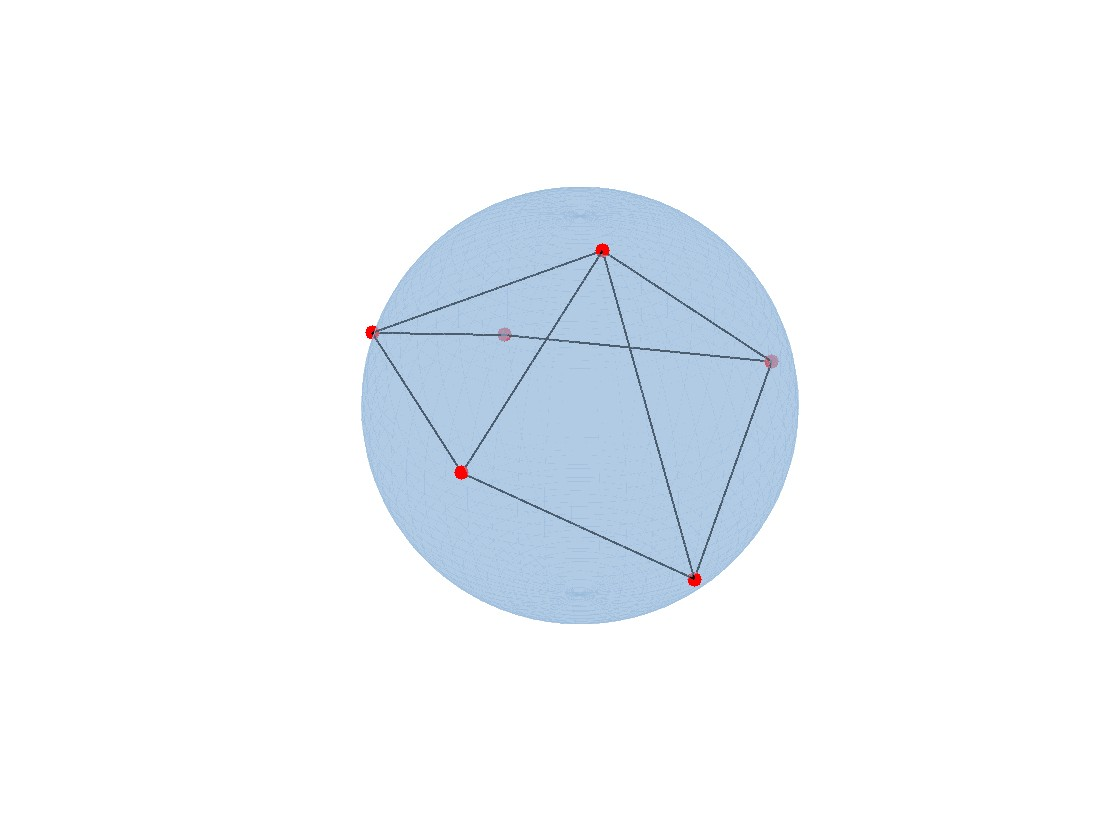
\includegraphics[width=\textwidth]{conf3_6_5.jpg}
        \caption{After $5$ iterations}
    \end{subfigure}
    \begin{subfigure}[b]{0.32\textwidth}
        \centering
        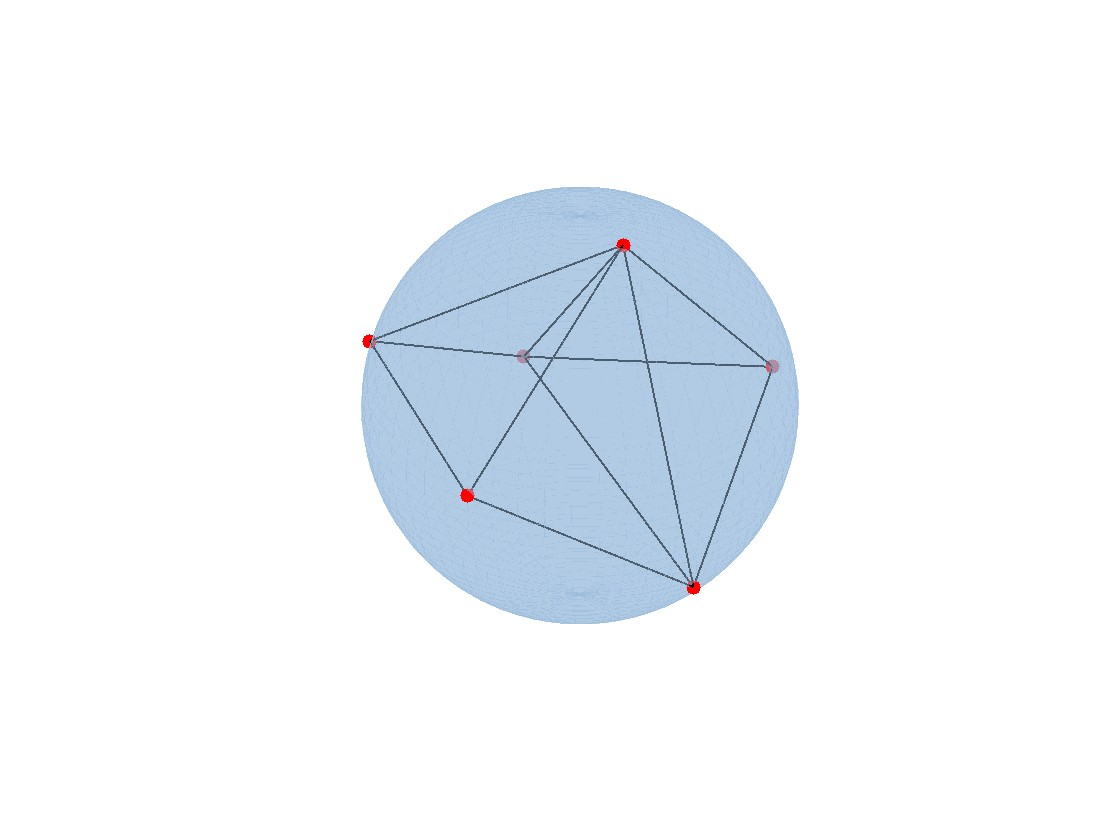
\includegraphics[width=\textwidth]{conf3_6_10.jpg}
        \caption{After $10$ iterations}
    \end{subfigure}

    % Deuxième ligne : 3 images
    \begin{subfigure}[b]{0.32\textwidth}
        \centering
        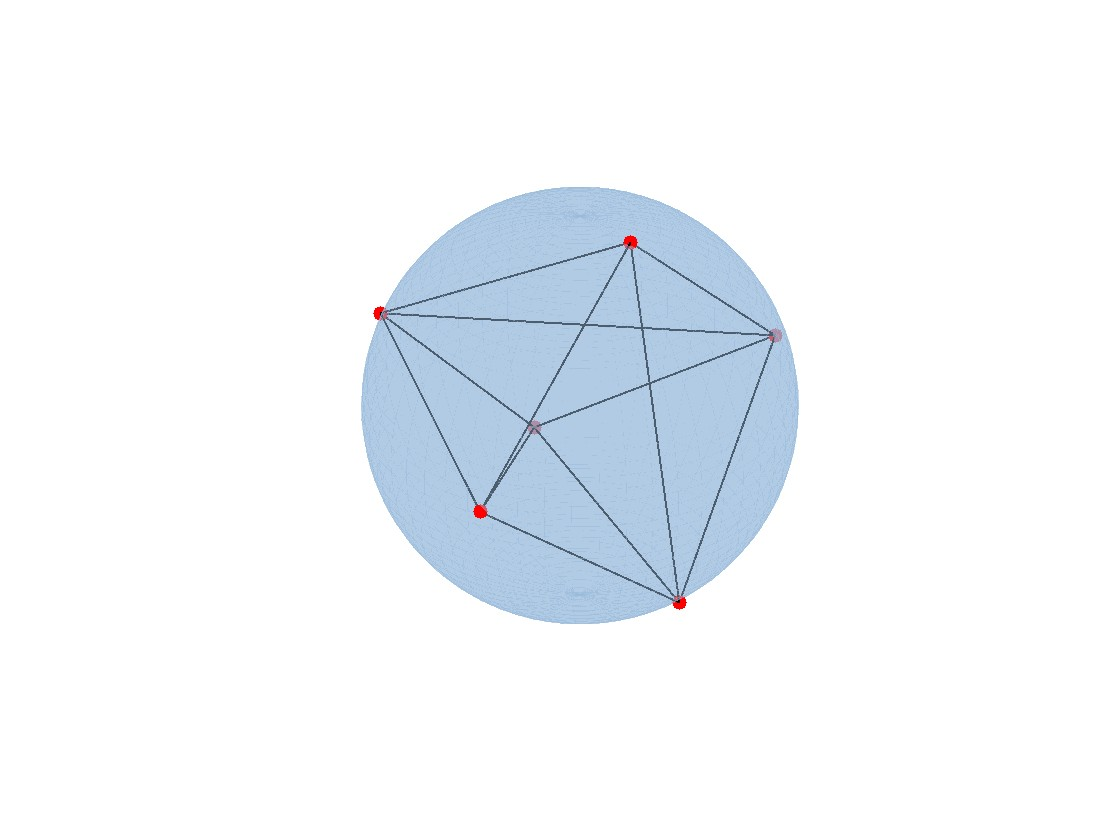
\includegraphics[width=\textwidth]{conf3_6_50.jpg}
        \caption{After $50$ iterations}
    \end{subfigure}
    \begin{subfigure}[b]{0.32\textwidth}
        \centering
        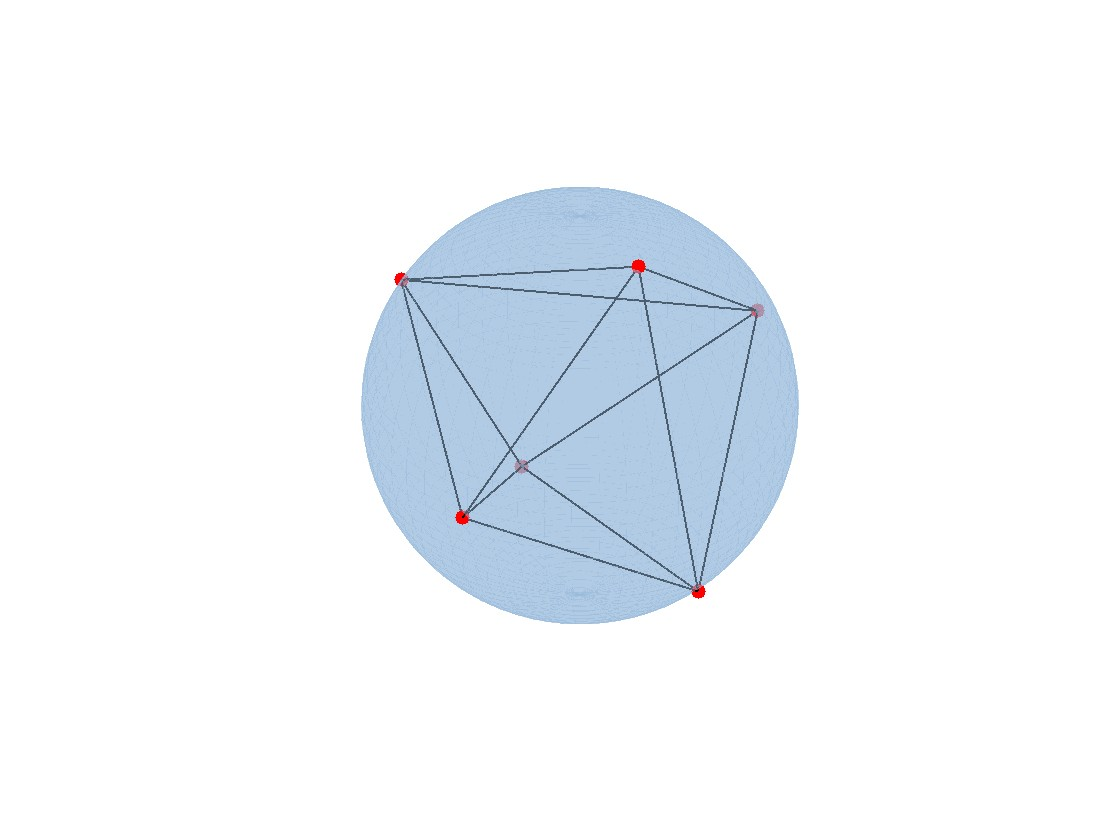
\includegraphics[width=\textwidth]{conf3_6_100.jpg}
        \caption{After $100$ iterations}
    \end{subfigure}
    \begin{subfigure}[b]{0.32\textwidth}
        \centering
        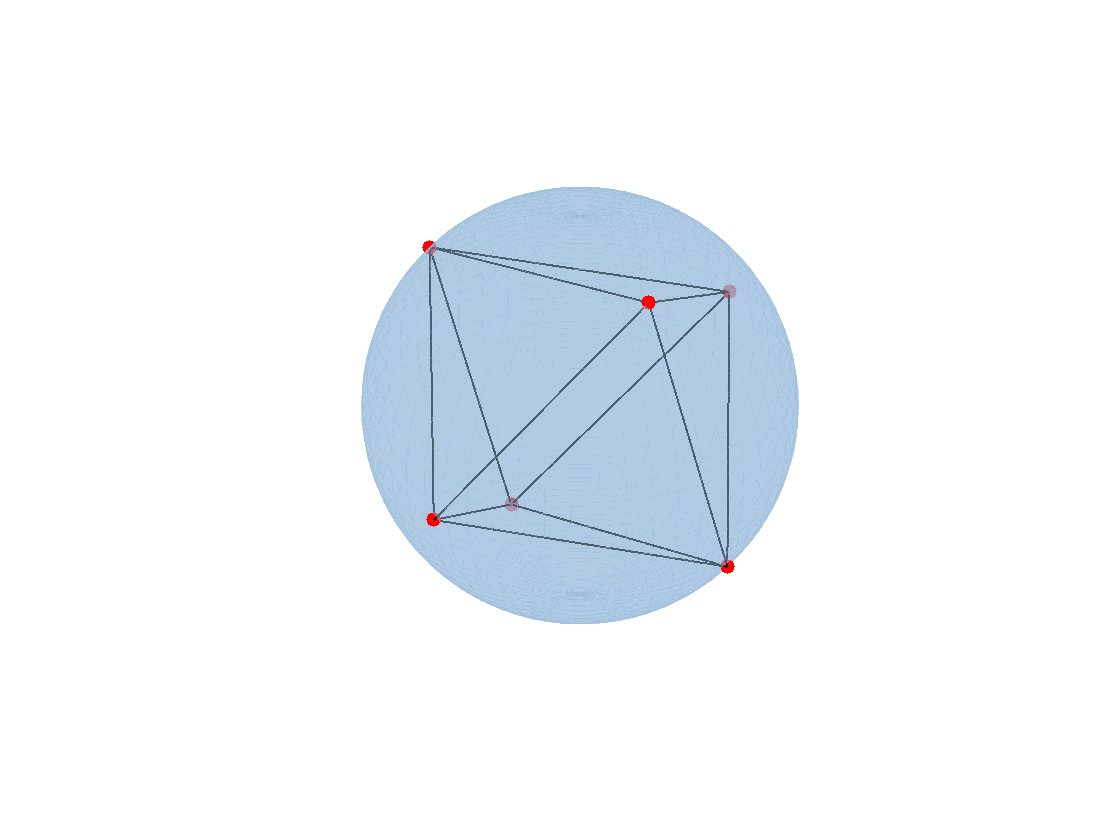
\includegraphics[width=\textwidth]{conf3_6_200.jpg}
        \caption{After $200$ iterations}
    \end{subfigure}

    % Troisième ligne : 1 image bien centrée
    \vspace{0.5cm} % Espace avant la dernière image
    \begin{subfigure}[b]{0.32\textwidth} % Plus large pour bien centrer
        \centering
        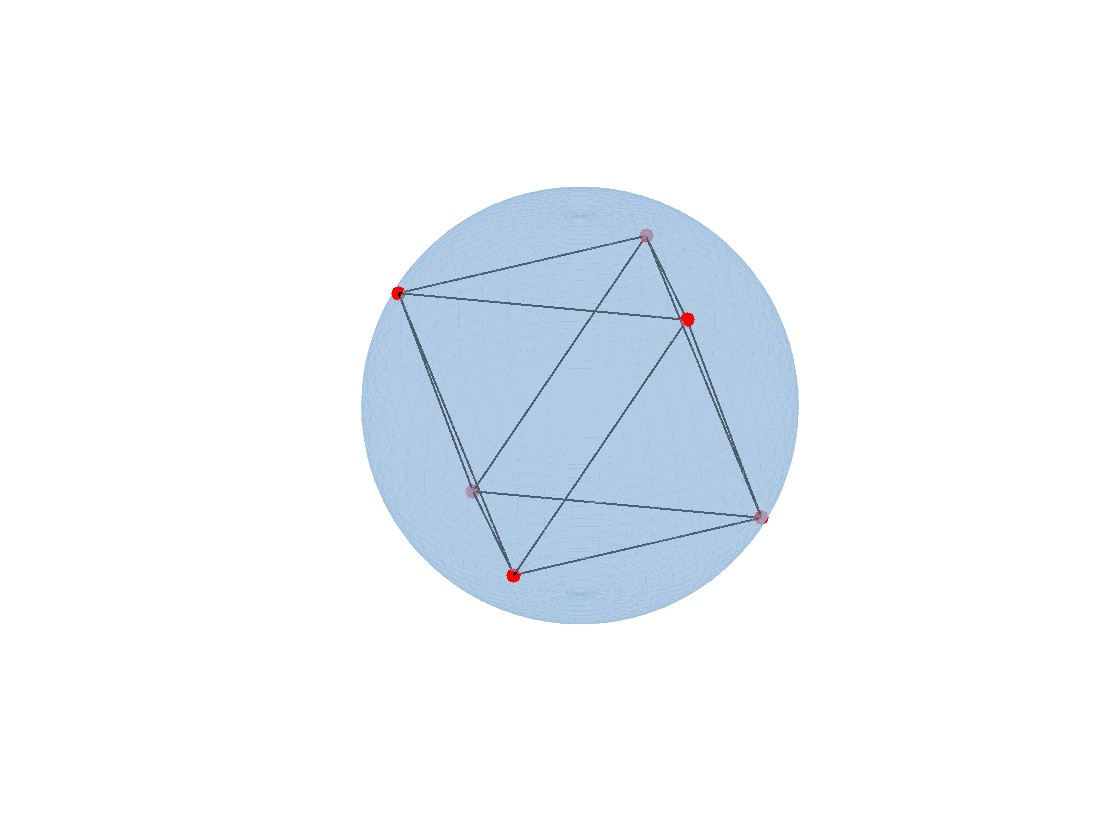
\includegraphics[width=\textwidth]{opt3_6.jpg}
        \caption{Best configuration obtained}
    \end{subfigure}

    \caption{Different configurations for $(3,6)$}
    \label{fig:conf3_6}
\end{figure}



\begin{figure}[H]
    \centering
    % Première ligne : 3 images
    \begin{subfigure}[b]{0.32\textwidth}
        \centering
        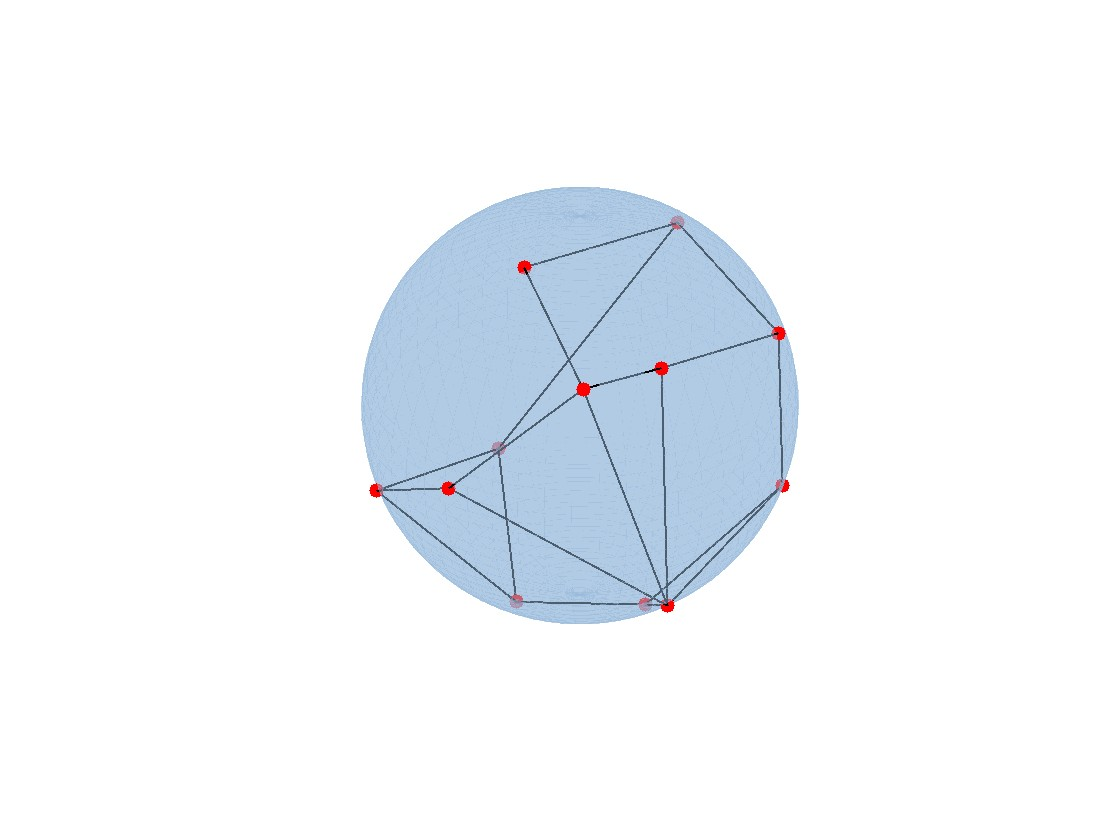
\includegraphics[width=\textwidth]{conf3_12_1.jpg}
        \caption{After $1$ iteration}
    \end{subfigure}
    \begin{subfigure}[b]{0.32\textwidth}
        \centering
        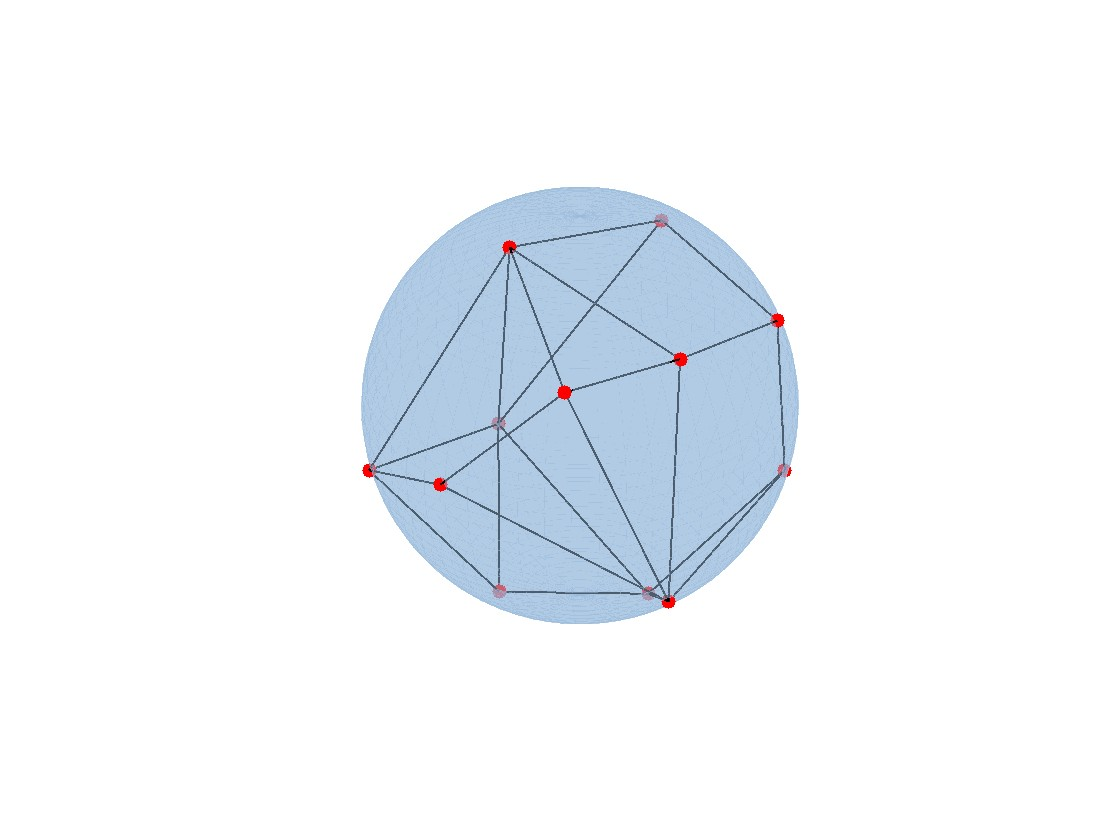
\includegraphics[width=\textwidth]{conf3_12_5.jpg}
        \caption{After $5$ iterations}
    \end{subfigure}
    \begin{subfigure}[b]{0.32\textwidth}
        \centering
        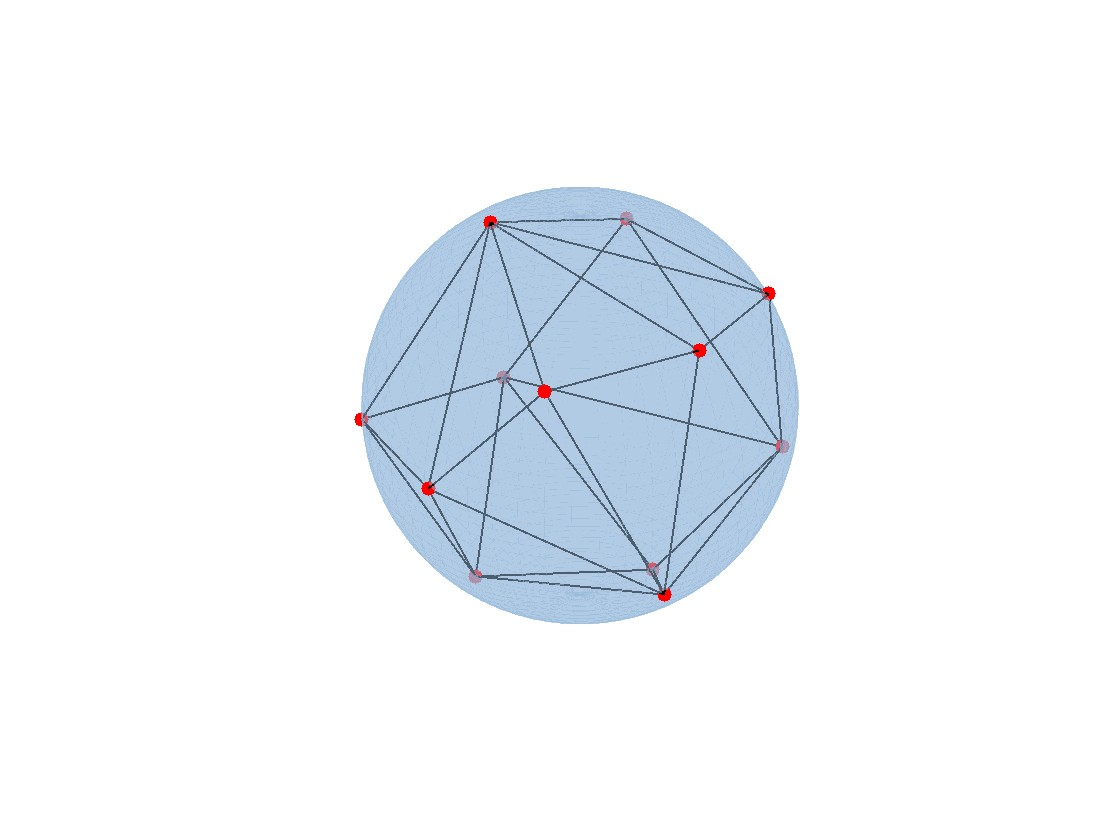
\includegraphics[width=\textwidth]{conf3_12_20.jpg}
        \caption{After $30$ iterations}
    \end{subfigure}

    % Deuxième ligne : 3 images
    \begin{subfigure}[b]{0.32\textwidth}
        \centering
        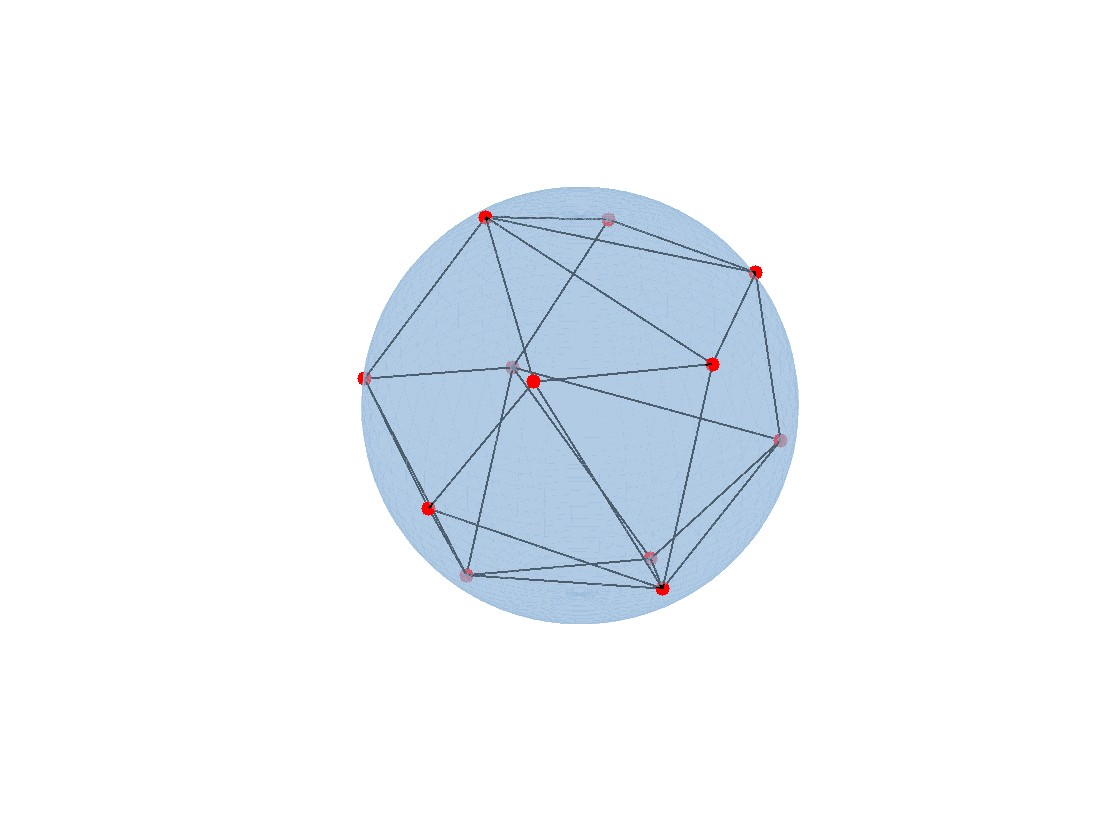
\includegraphics[width=\textwidth]{conf3_12_50.jpg}
        \caption{After $50$ iterations}
    \end{subfigure}
    \begin{subfigure}[b]{0.32\textwidth}
        \centering
        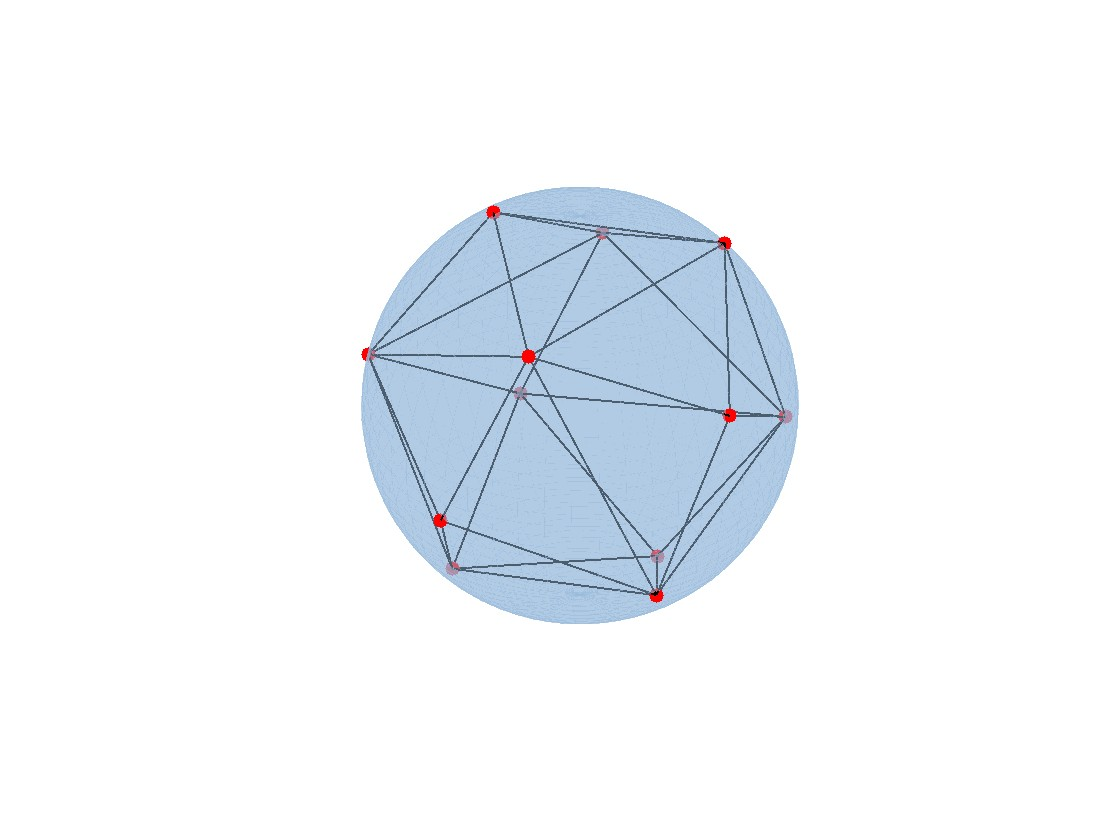
\includegraphics[width=\textwidth]{conf3_12_200.jpg}
        \caption{After $100$ iterations}
    \end{subfigure}
    \begin{subfigure}[b]{0.32\textwidth}
        \centering
        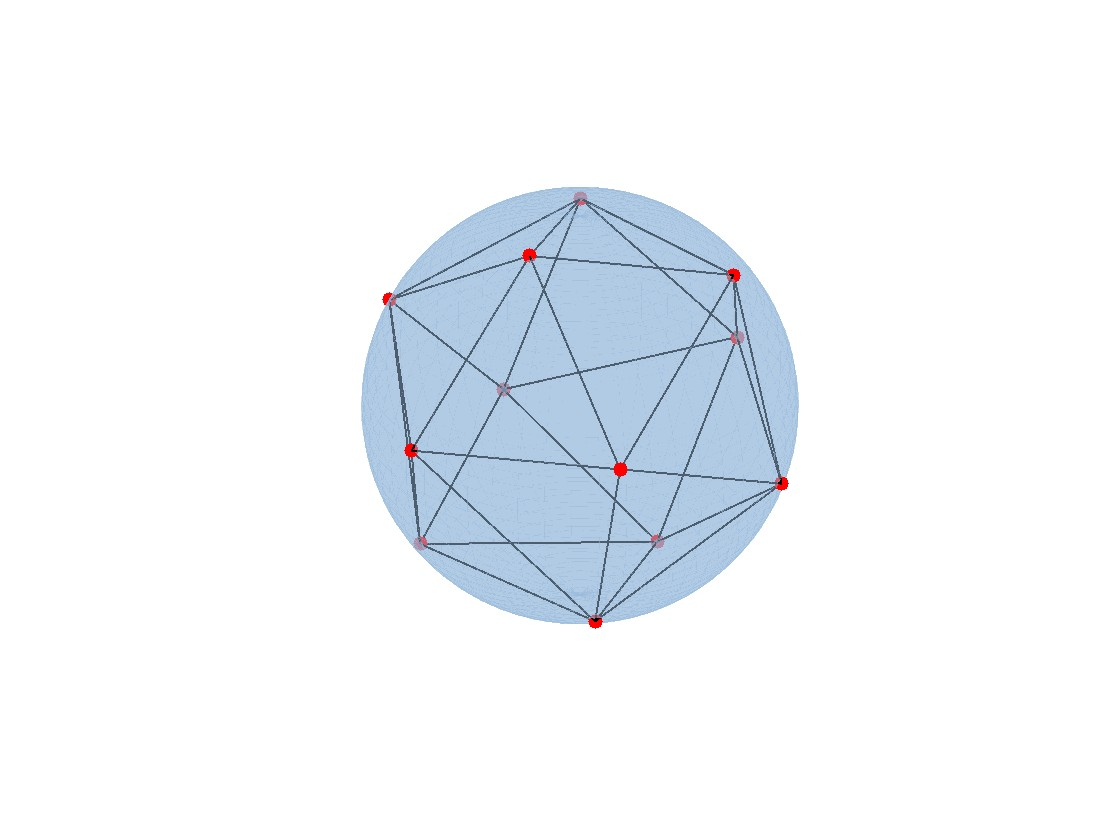
\includegraphics[width=\textwidth]{opt3_12.jpg}
        \caption{Best configuration obtained}
    \end{subfigure}

    \caption{Different configurations for $(3,12)$}
    \label{fig:conf3_12}
\end{figure}



\begin{figure}[H]
    \centering
    % Première ligne : 3 images
    \begin{subfigure}[b]{0.32\textwidth}
        \centering
        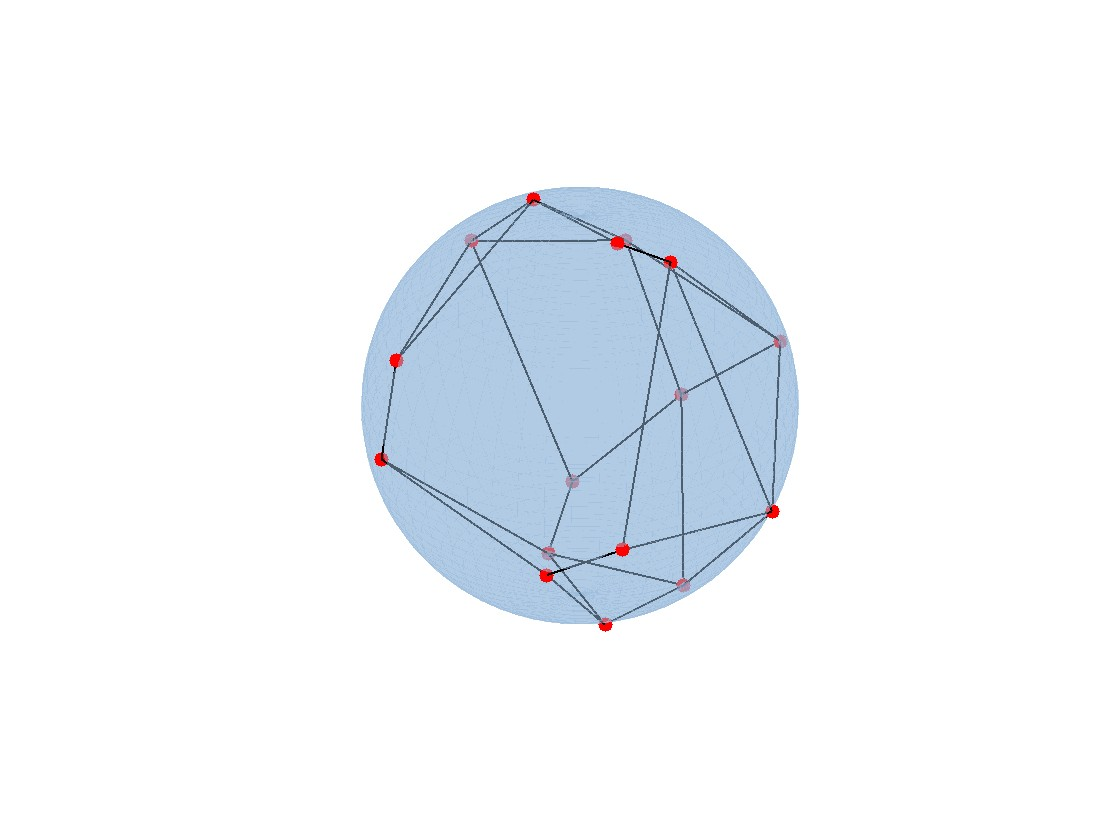
\includegraphics[width=\textwidth]{conf3_16_1.jpg}
        \caption{After $1$ iteration}
    \end{subfigure}
    \begin{subfigure}[b]{0.32\textwidth}
        \centering
        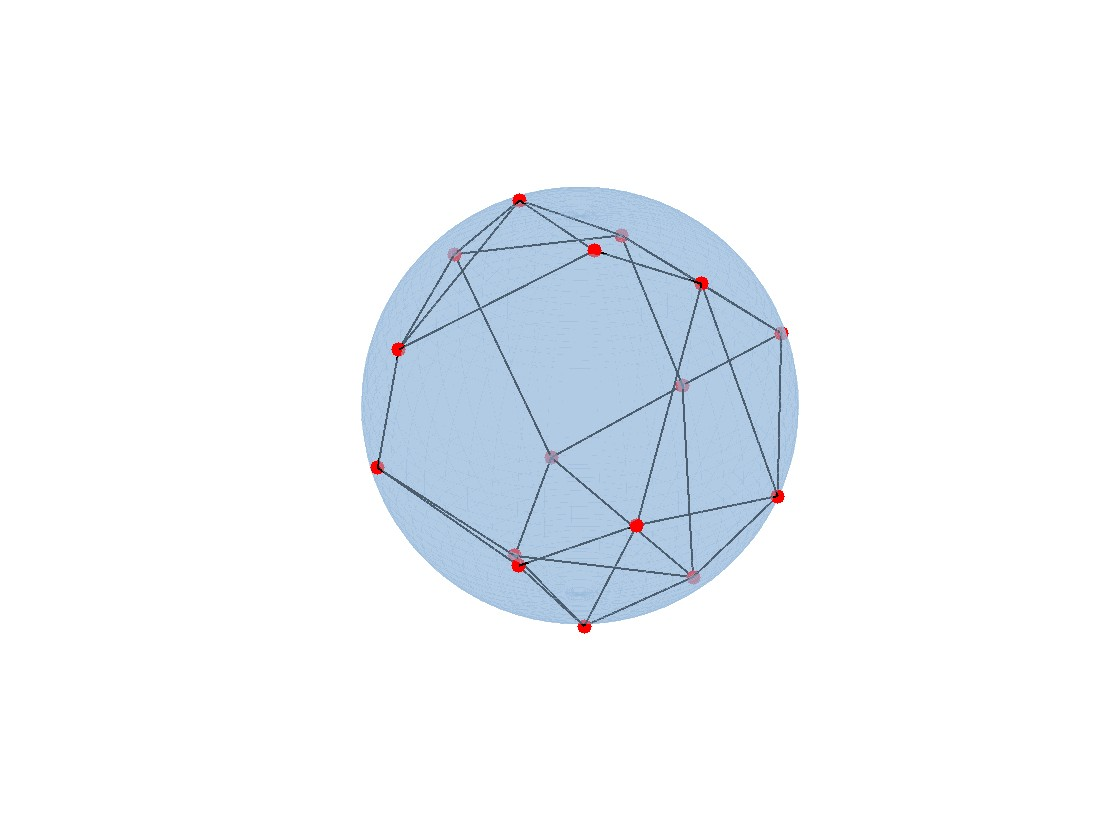
\includegraphics[width=\textwidth]{conf3_16_10.jpg}
        \caption{After $10$ iterations}
    \end{subfigure}
    \begin{subfigure}[b]{0.32\textwidth}
        \centering
        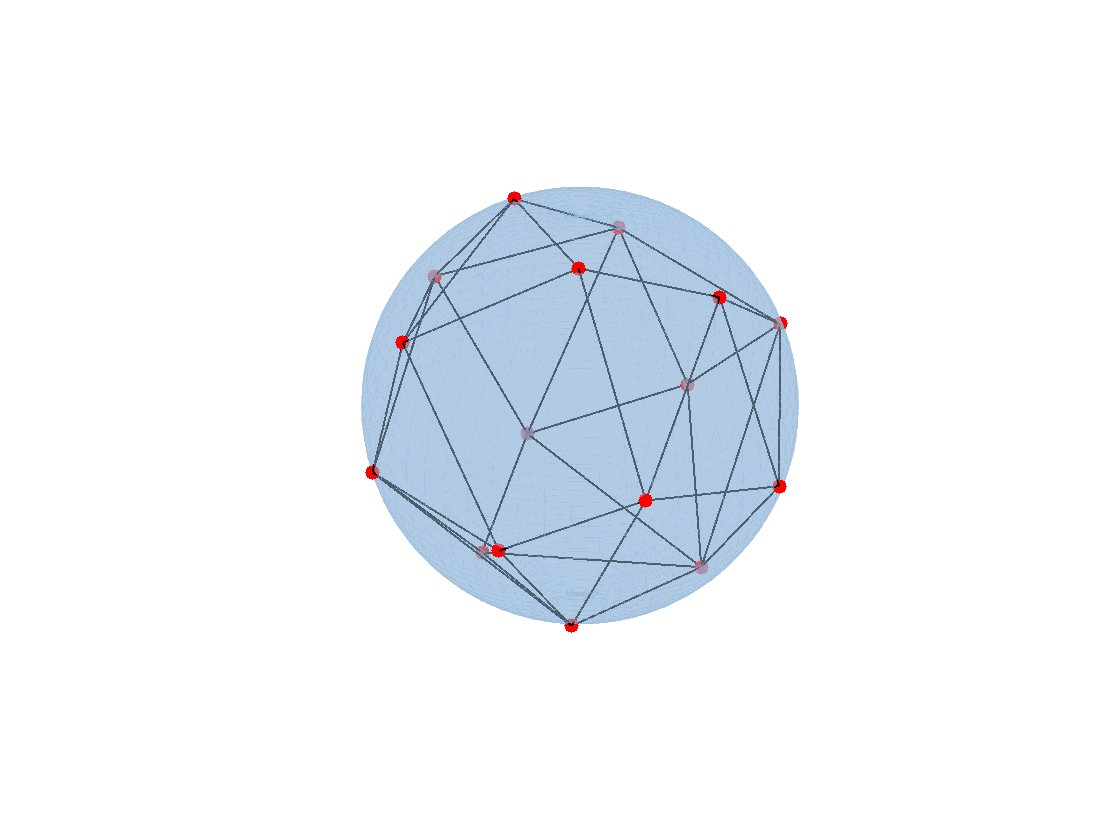
\includegraphics[width=\textwidth]{conf3_16_30.jpg}
        \caption{After $30$ iterations}
    \end{subfigure}

    % Deuxième ligne : 3 images
    \begin{subfigure}[b]{0.32\textwidth}
        \centering
        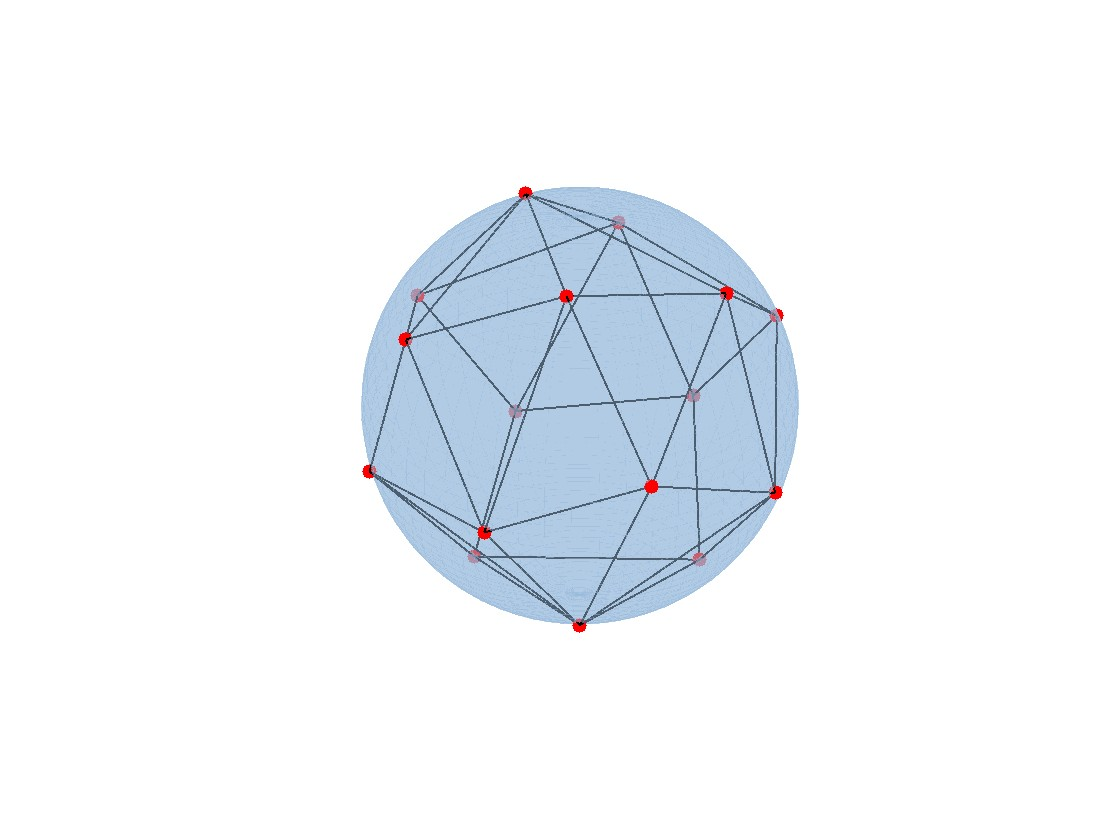
\includegraphics[width=\textwidth]{conf3_16_100.jpg}
        \caption{After $100$ iterations}
    \end{subfigure}
    \begin{subfigure}[b]{0.32\textwidth}
        \centering
        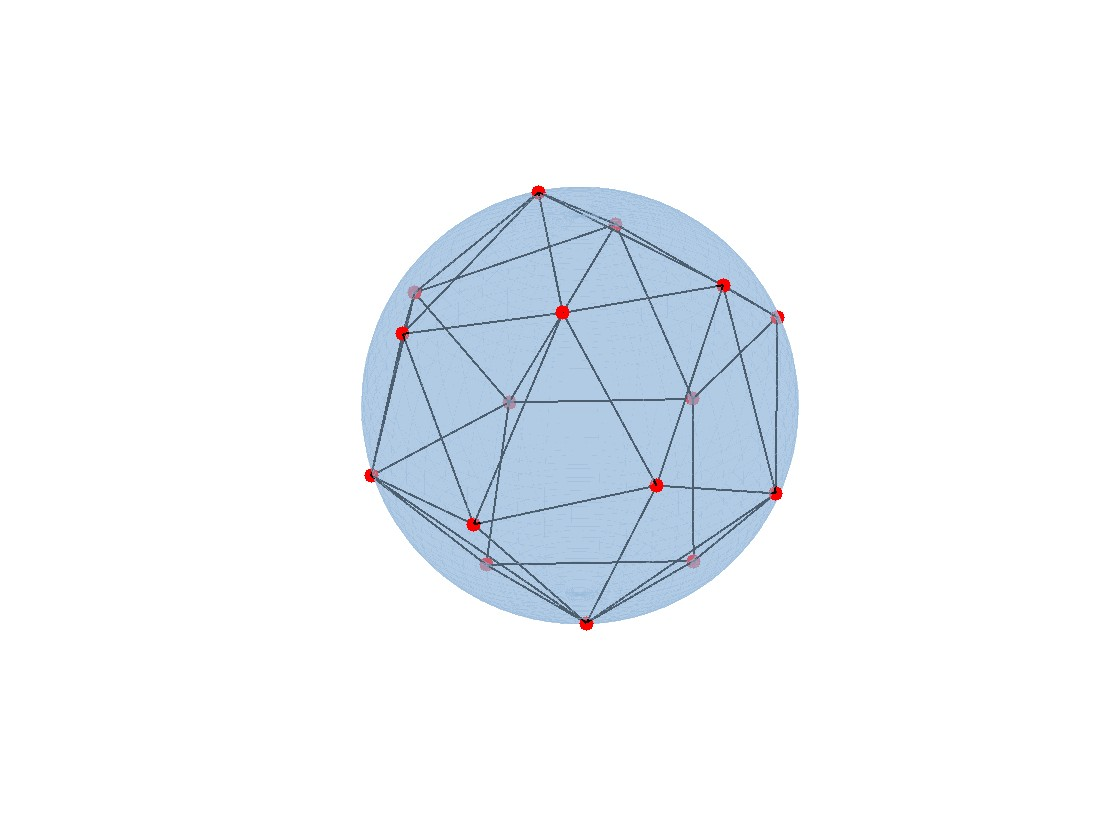
\includegraphics[width=\textwidth]{conf3_16_200.jpg}
        \caption{After $200$ iterations}
    \end{subfigure}
    \begin{subfigure}[b]{0.32\textwidth}
        \centering
        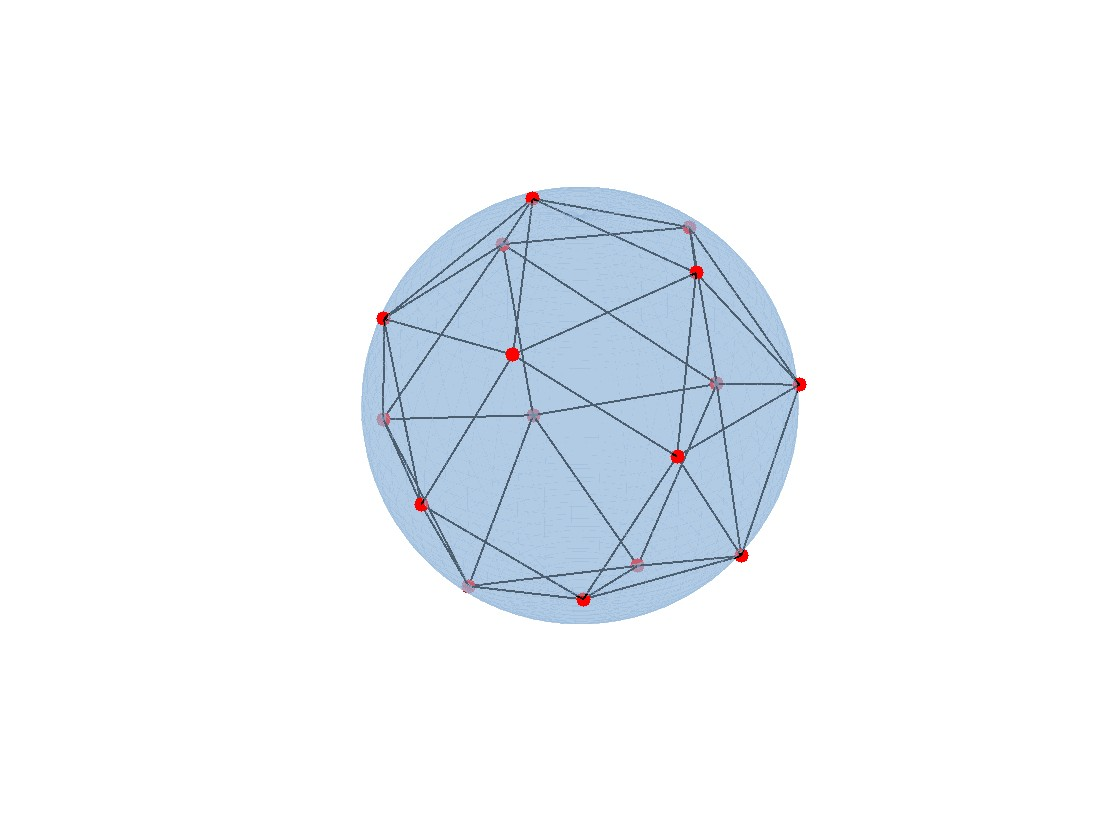
\includegraphics[width=\textwidth]{opt3_16.jpg}
        \caption{Best configuration obtained}
    \end{subfigure}

    \caption{Different configurations for $(3,16)$}
    \label{fig:conf3_16}
\end{figure}

Finally, for pairs $(2, 100)$ and $(3, 128)$, we give the plots of the function values and gradient norms (in log scale) as a function of the iteration number obtained while running the $30$ experiments, for the best configurations. Figure \ref{fig:2315} gives such graphs for the pair $(2, 100)$. We notice that $f$ decays exponentially fast to the minimum value. Although there has not been convergence, due to the norm of the gradient not being small enough, the function $f$ has considerably decreased after $250$ iterations and stabilized. As for the gradient norm, we notice that it starts by decreasing exponentially within the first iterations and decays then almost linearly (on the log scale) in the number of iterations.

%\begin{figure}[H]
    %\centering
    %\begin{subfigure}[b]{0.45\textwidth}
    %    \centering
    %    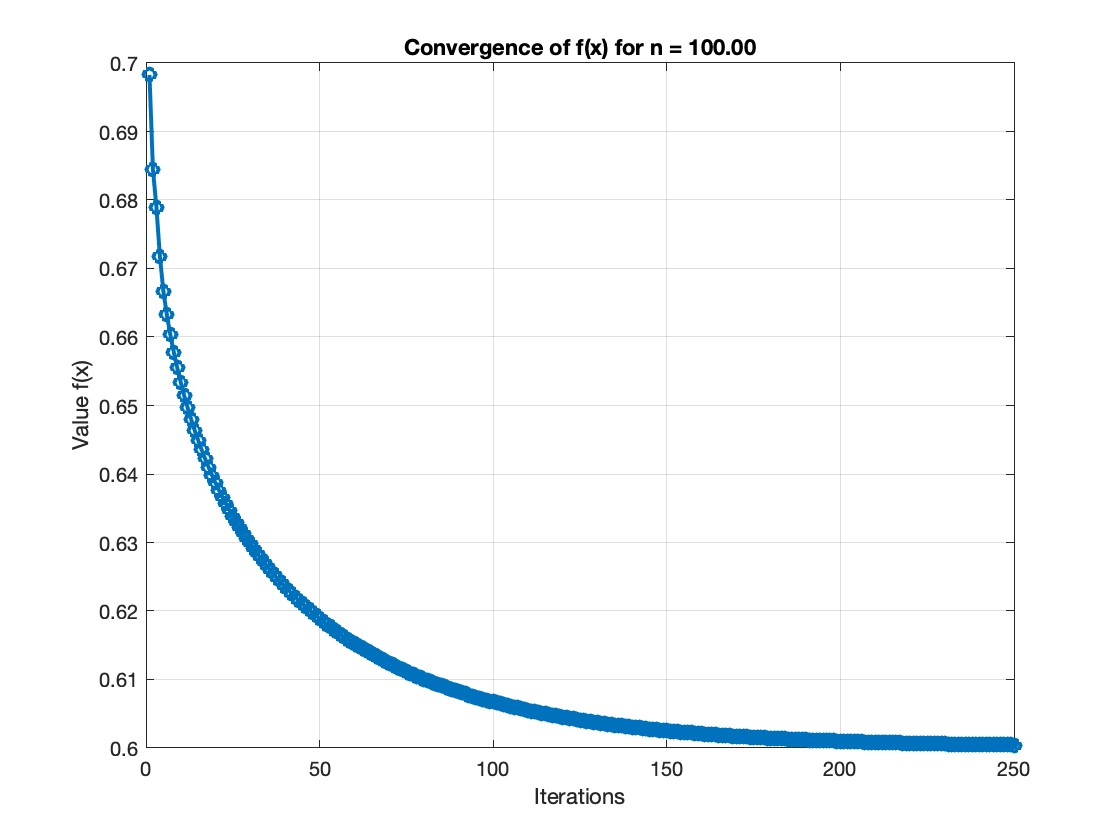
\includegraphics[width=\textwidth]{23f1.jpg}
    %\end{subfigure}
    %\begin{subfigure}[b]{0.45\textwidth}
    %    \centering
    %    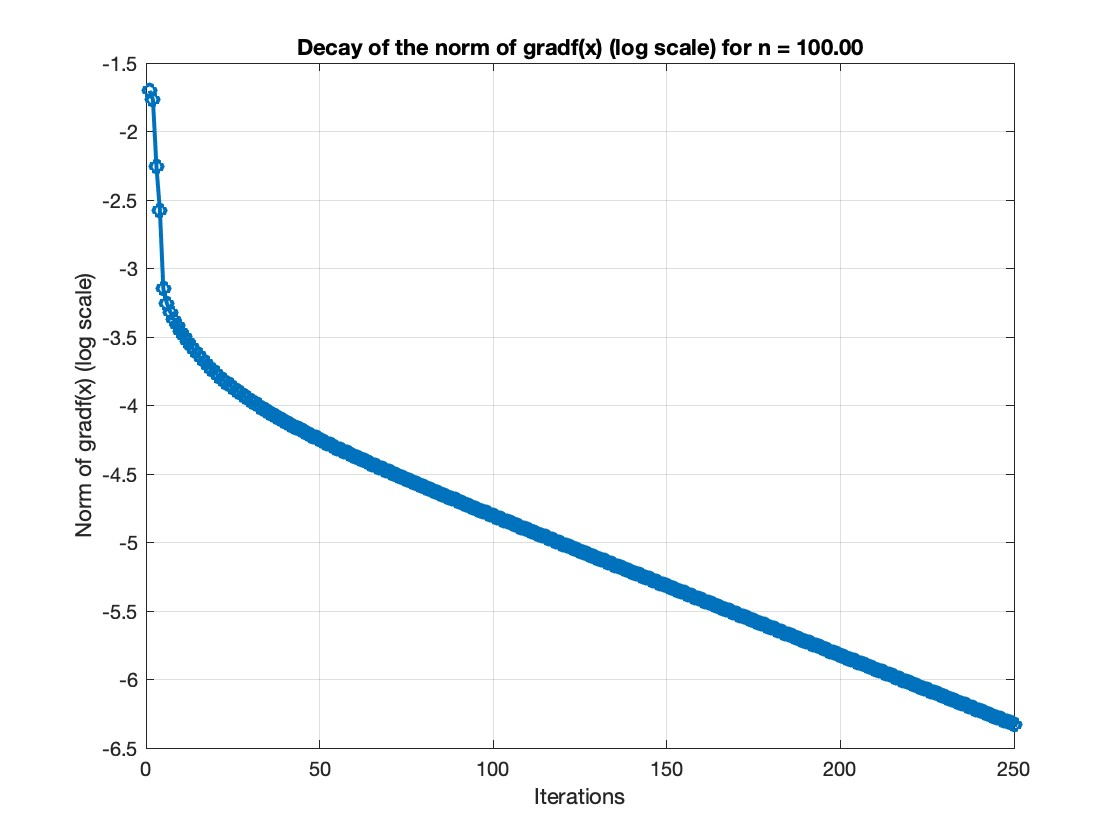
\includegraphics[width=\textwidth]{23g1}
    %\end{subfigure}
    %\caption{Experiment $1$ for $(2, 100)$}
    %\label{fig:231}
    
    %\newpage

    %\begin{subfigure}[b]{0.45\textwidth}
    %    \centering
    %    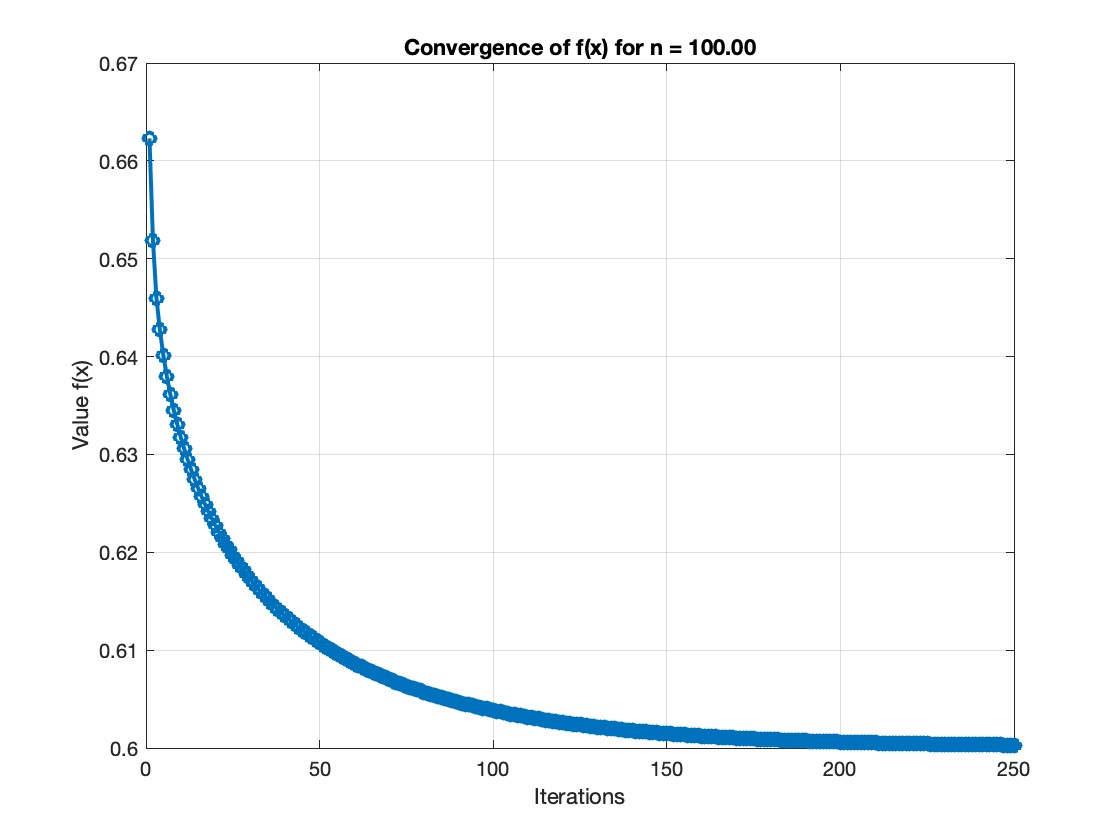
\includegraphics[width=\textwidth]{23f2.jpg}
    %\end{subfigure}
    %\begin{subfigure}[b]{0.45\textwidth}
    %    \centering
    %    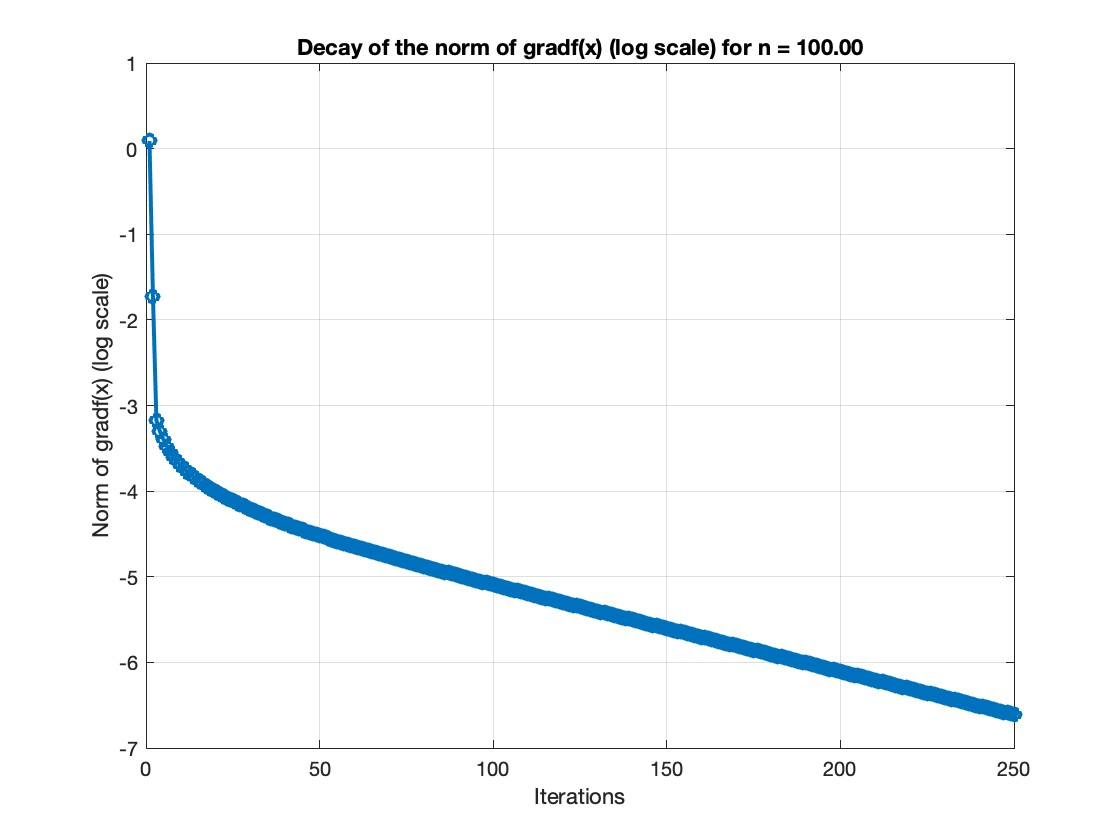
\includegraphics[width=\textwidth]{23g2.jpg}
    %\end{subfigure}
    %\caption{Experiment $2$ for $(2, 100)$}
    
    %\newpage

    %\begin{subfigure}[b]{0.45\textwidth}
    %    \centering
    %    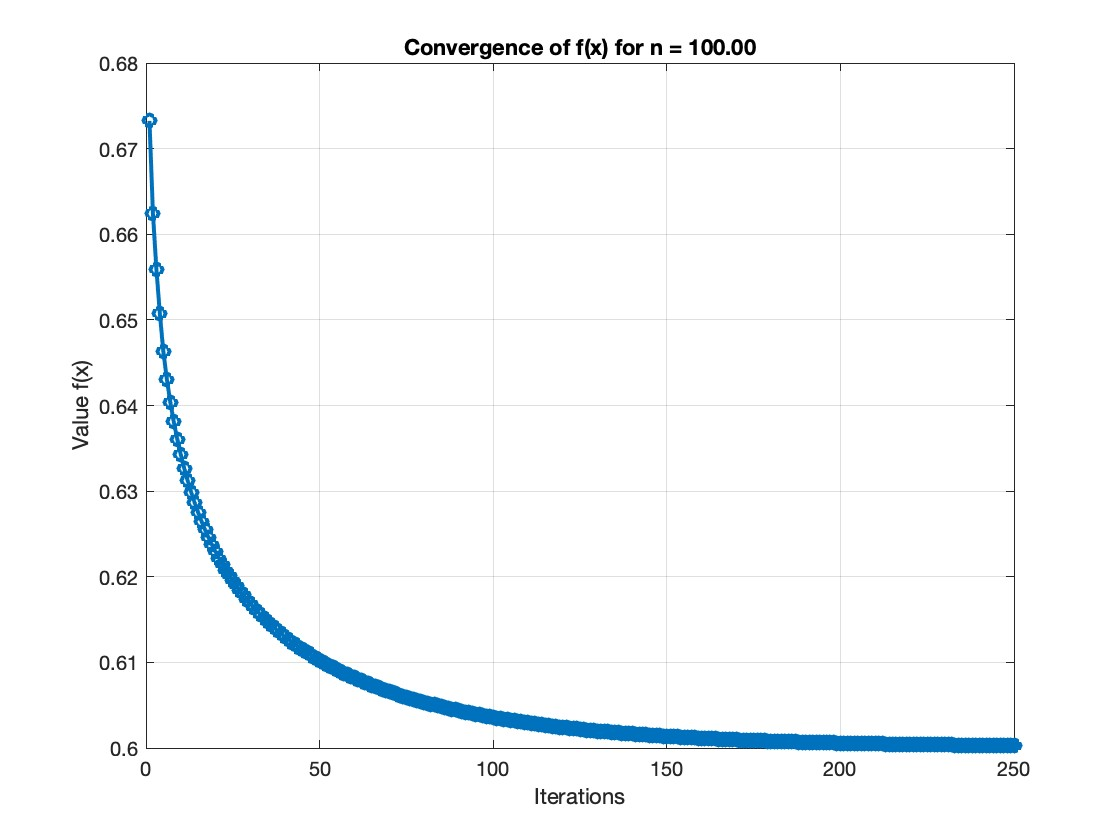
\includegraphics[width=\textwidth]{23f3.jpg}
    %\end{subfigure}
    %\begin{subfigure}[b]{0.45\textwidth}
    %    \centering
    %    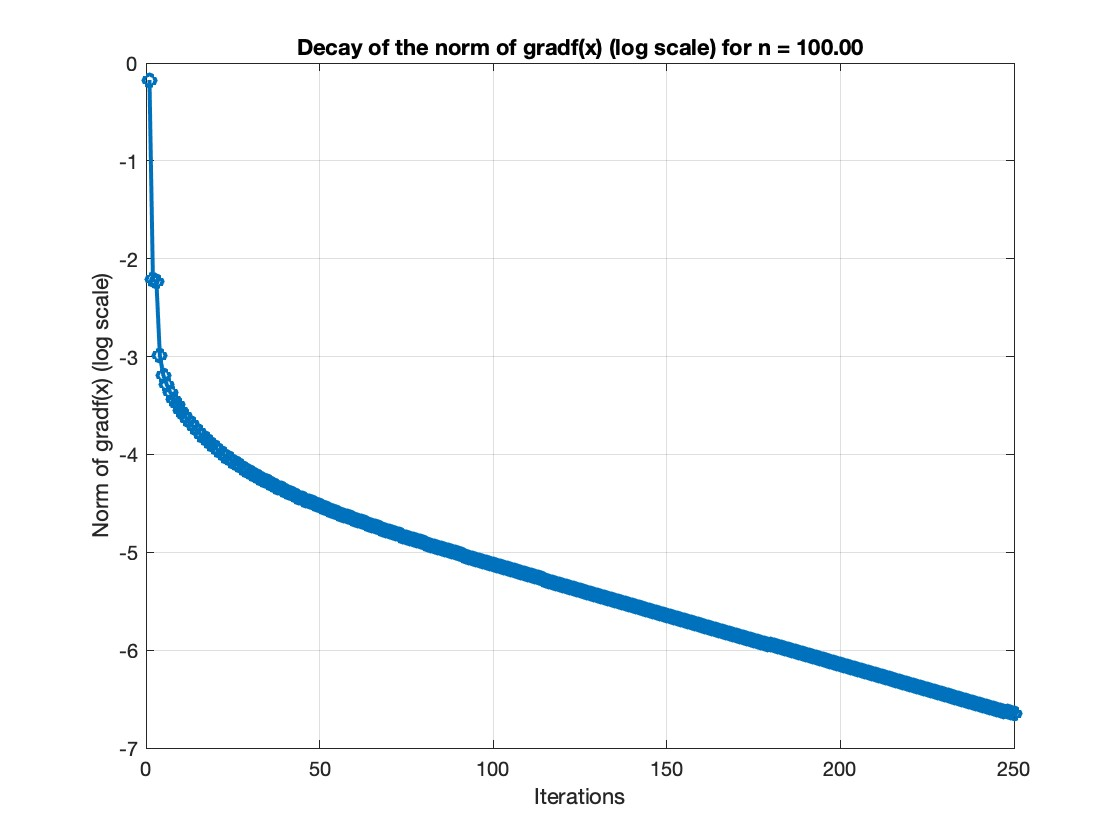
\includegraphics[width=\textwidth]{23g3.jpg}
    %\end{subfigure}
    %\caption{Experiment $3$ for $(2, 100)$}

    %\newpage

    %\begin{subfigure}[b]{0.45\textwidth}
    %    \centering
    %    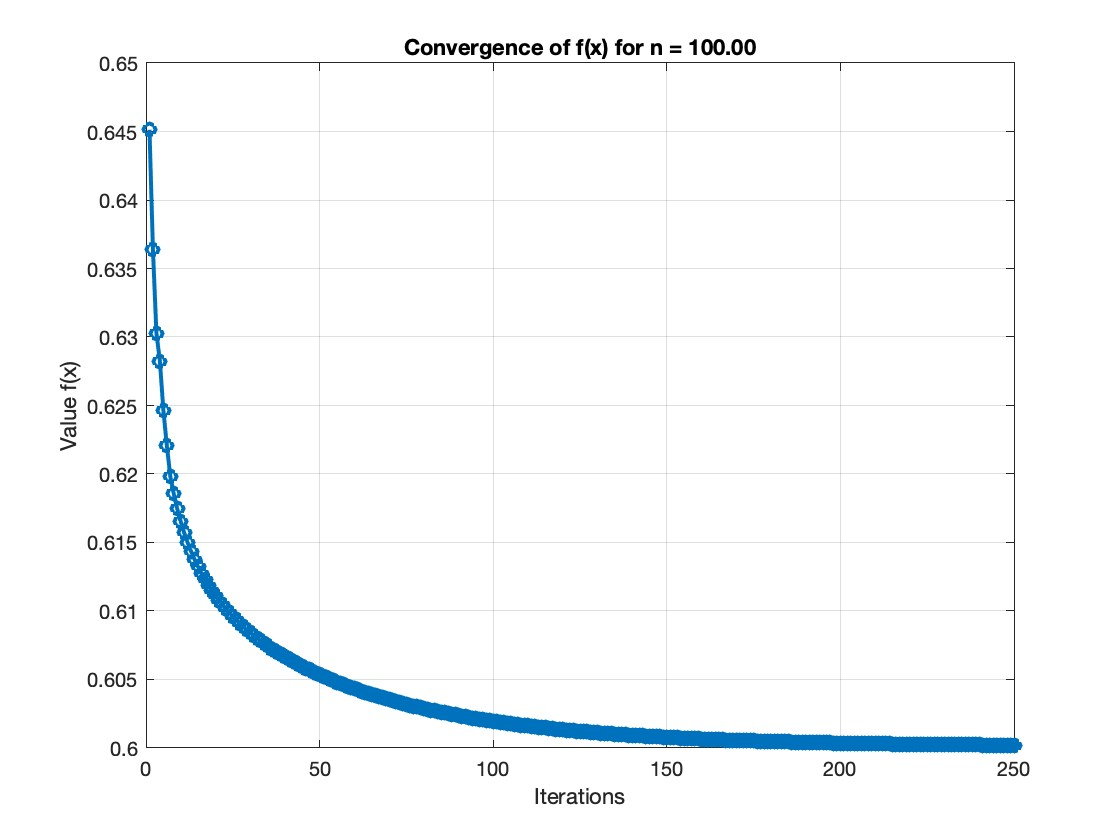
\includegraphics[width=\textwidth]{23f4.jpg}
    %\end{subfigure}
    %\begin{subfigure}[b]{0.45\textwidth}
    %    \centering
    %    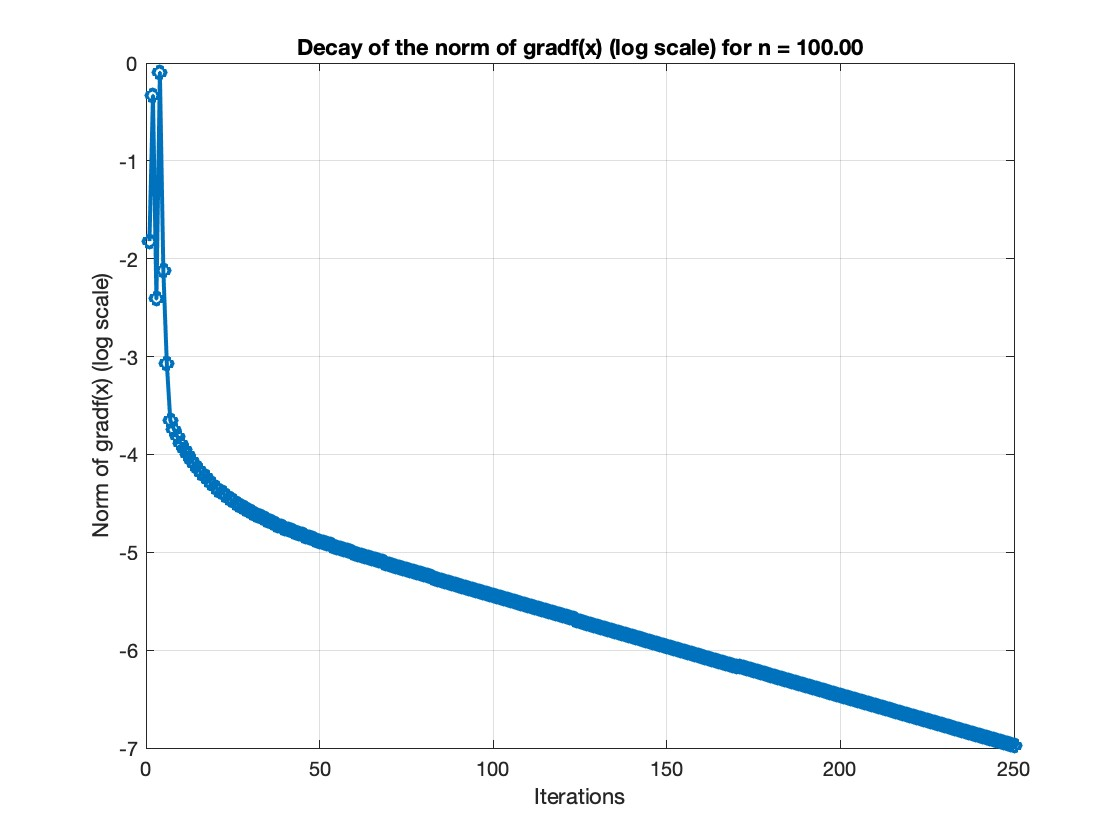
\includegraphics[width=\textwidth]{23g4.jpg}
    %\end{subfigure}
    %\caption{Experiment $4$ for $(2, 100)$}
%\end{figure}
%\begin{figure}
%    \centering
%    \begin{subfigure}[b]{0.45\textwidth}
%        \centering
%        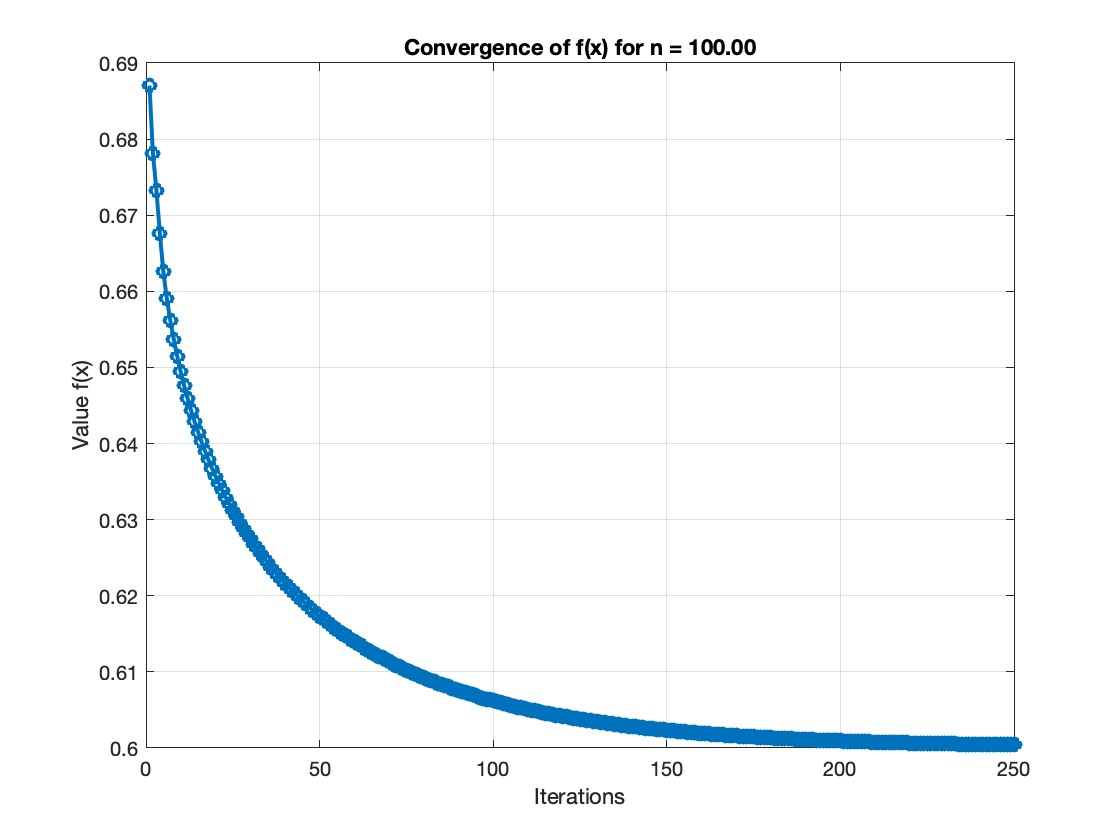
\includegraphics[width=\textwidth]{23f5.jpg}
%    \end{subfigure}
%    \begin{subfigure}[b]{0.45\textwidth}
%        \centering
%        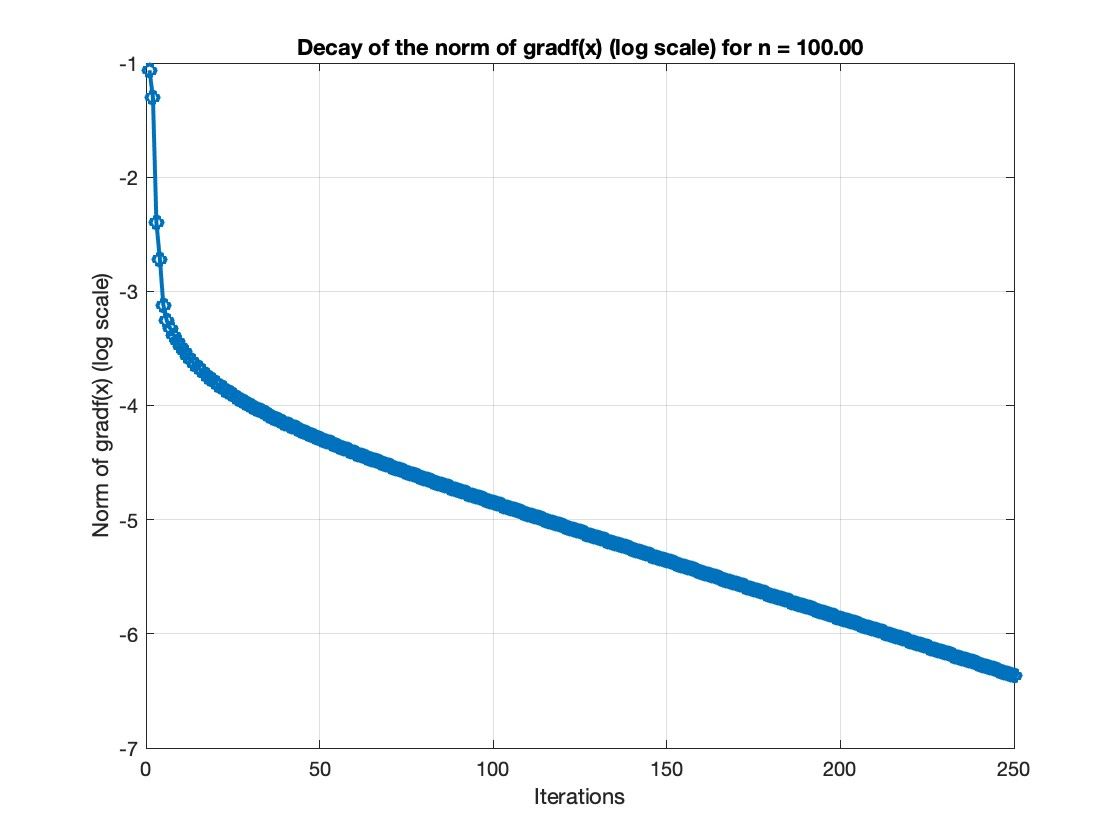
\includegraphics[width=\textwidth]{23g5.jpg}
%    \end{subfigure}
%    \caption{Experiment $5$ for $(2, 100)$}

%    \newpage
%
%    \begin{subfigure}[b]{0.45\textwidth}
%        \centering
%        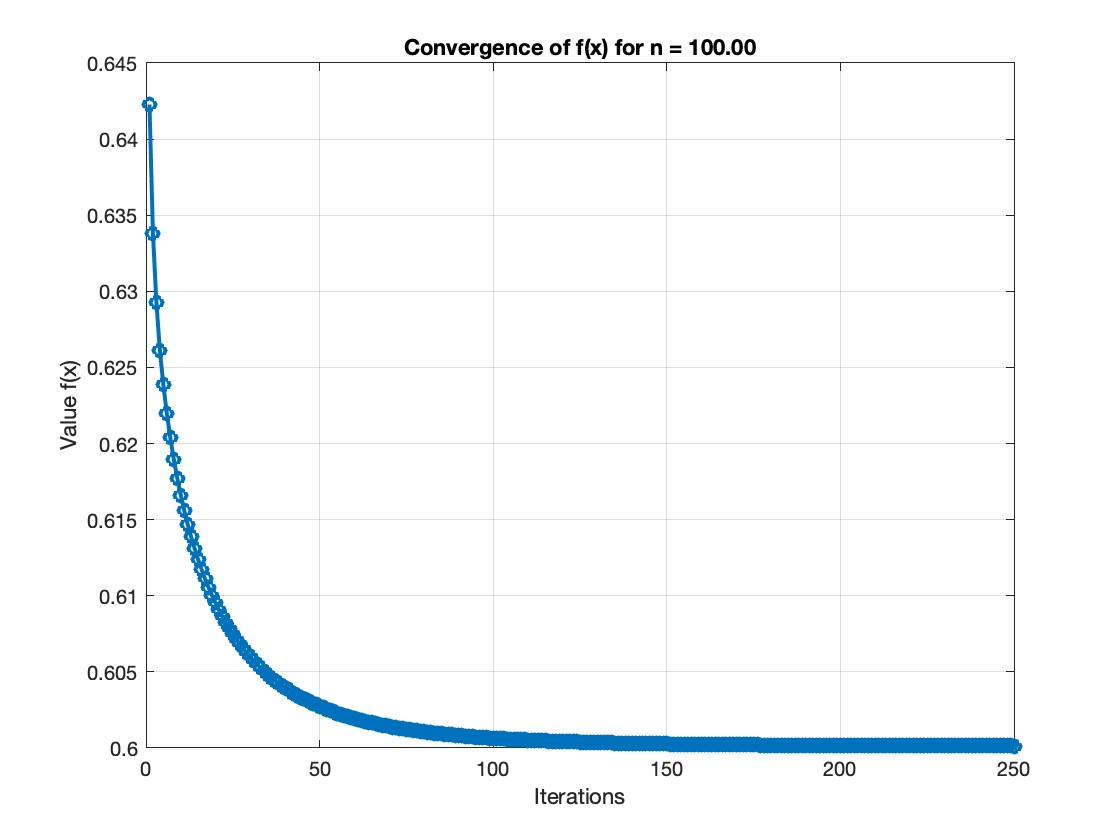
\includegraphics[width=\textwidth]{23f6.jpg}
%    \end{subfigure}
%    \begin{subfigure}[b]{0.45\textwidth}
%        \centering
%        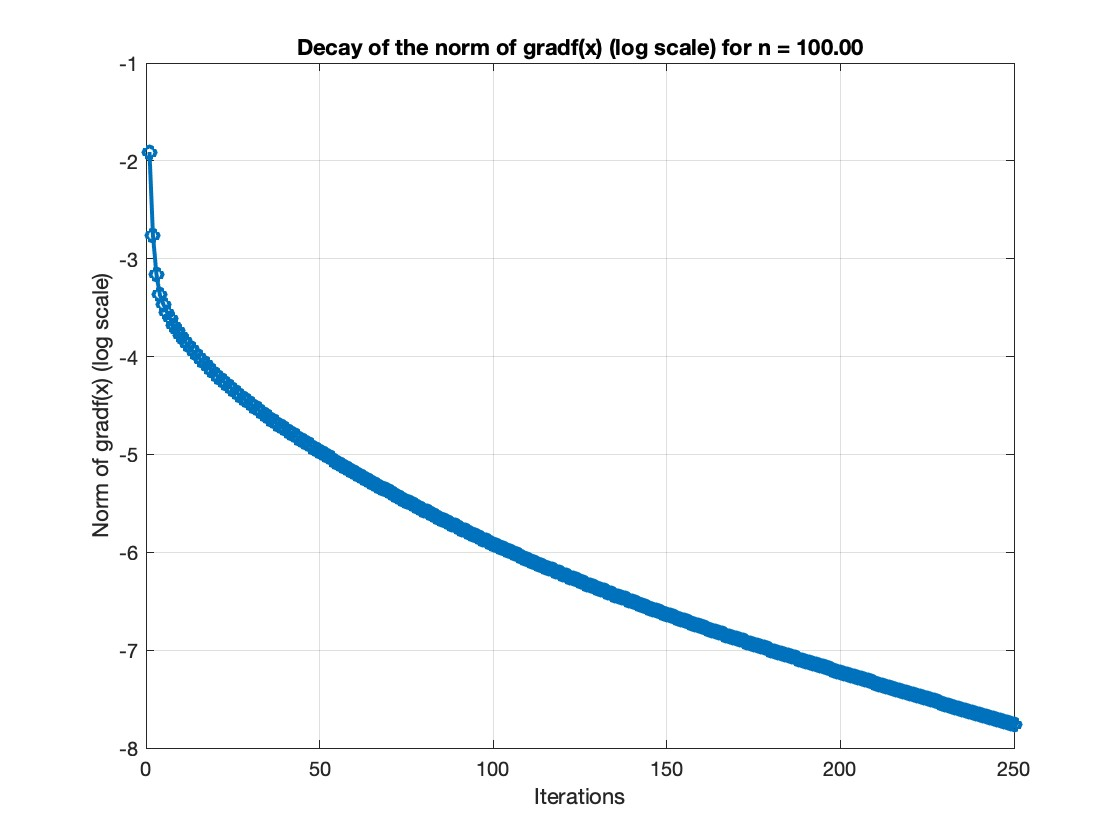
\includegraphics[width=\textwidth]{23g6.jpg}
%    \end{subfigure}
%    \caption{Experiment $6$ for $(2, 100)$}

 %   \newpage

%    \begin{subfigure}[b]{0.45\textwidth}
%        \centering
%        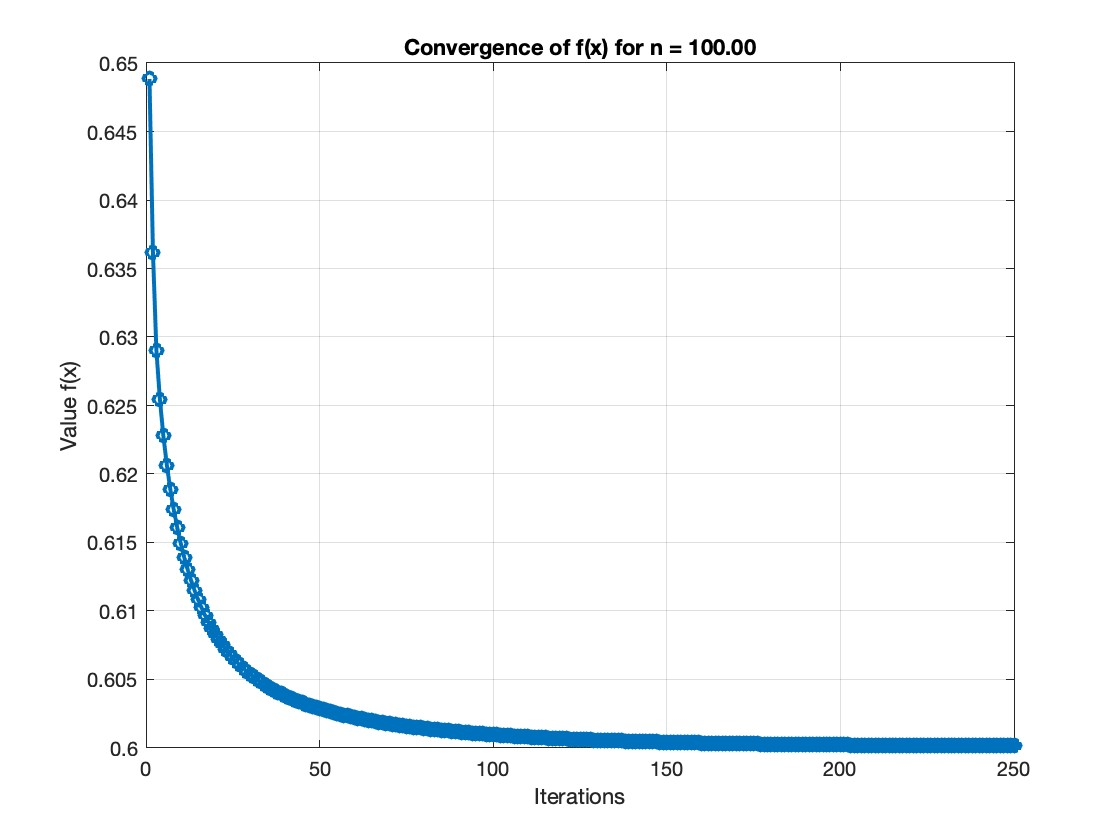
\includegraphics[width=\textwidth]{23f7.jpg}
%    \end{subfigure}
%    \begin{subfigure}[b]{0.45\textwidth}
%        \centering
%        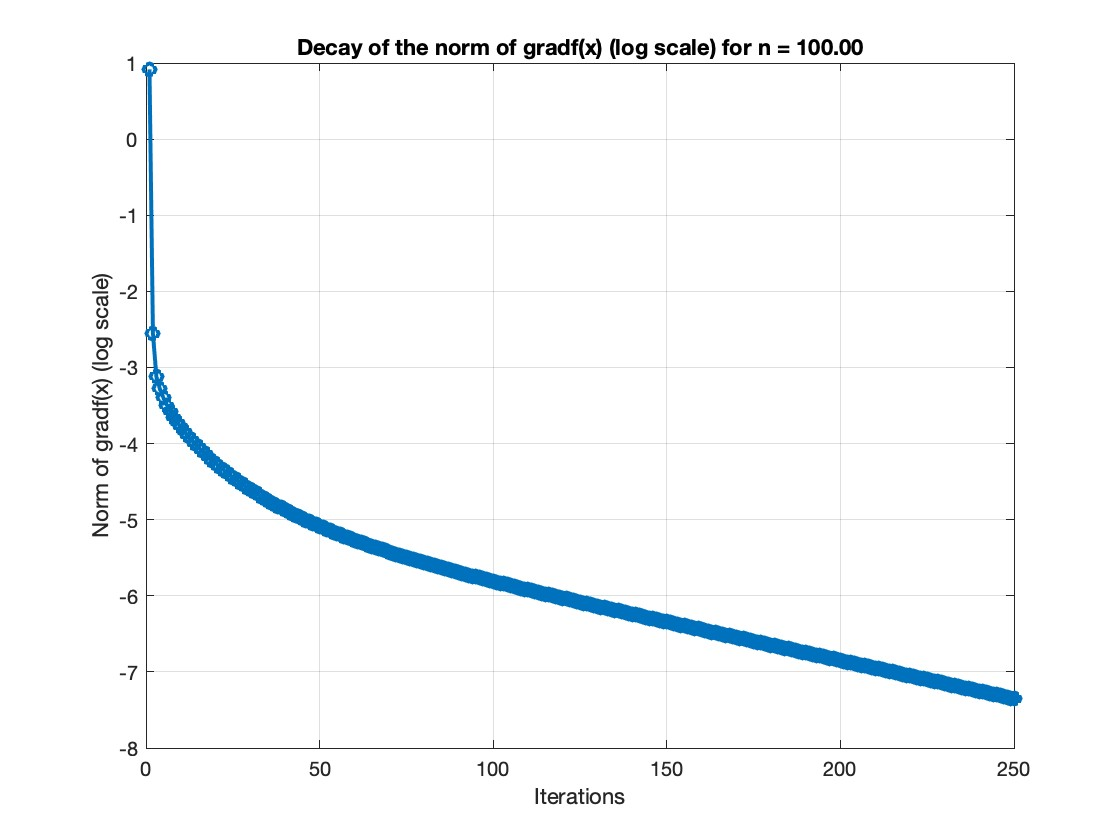
\includegraphics[width=\textwidth]{23g7.jpg}
%    \end{subfigure}
%    \caption{Experiment $7$ for $(2, 100)$}

%    \newpage

%    \begin{subfigure}[b]{0.45\textwidth}
%        \centering
%        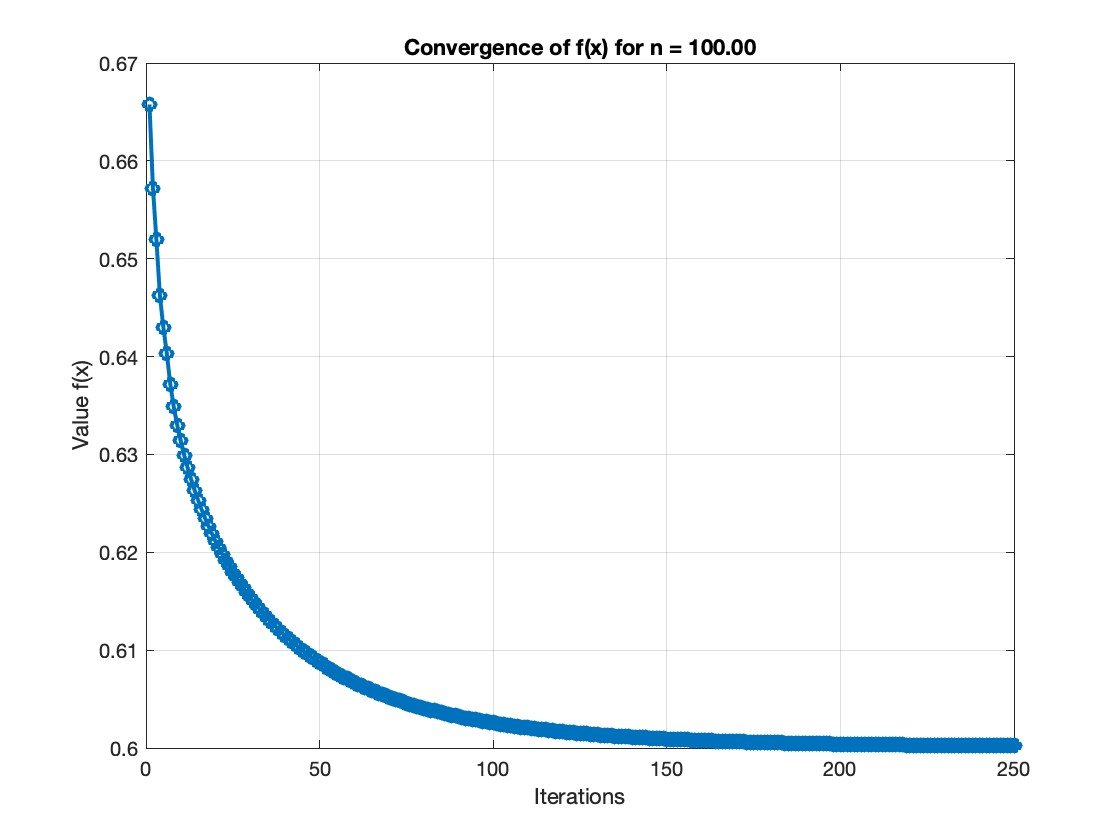
\includegraphics[width=\textwidth]{23f8.jpg}
%    \end{subfigure}
%    \begin{subfigure}[b]{0.45\textwidth}
%        \centering
%        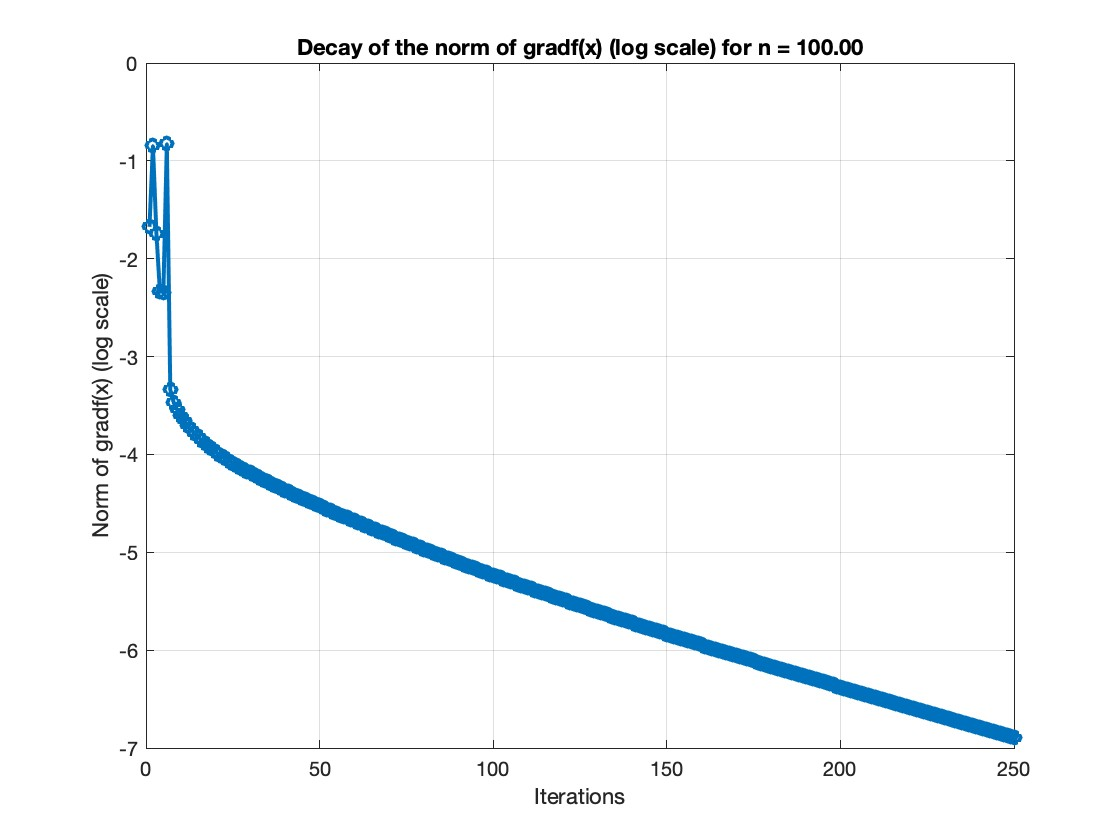
\includegraphics[width=\textwidth]{23g8.jpg}
%    \end{subfigure}
%    \caption{Experiment $8$ for $(2, 100)$}
%\end{figure}
%\begin{figure}
%    \centering
%    \begin{subfigure}[b]{0.45\textwidth}
%        \centering
%        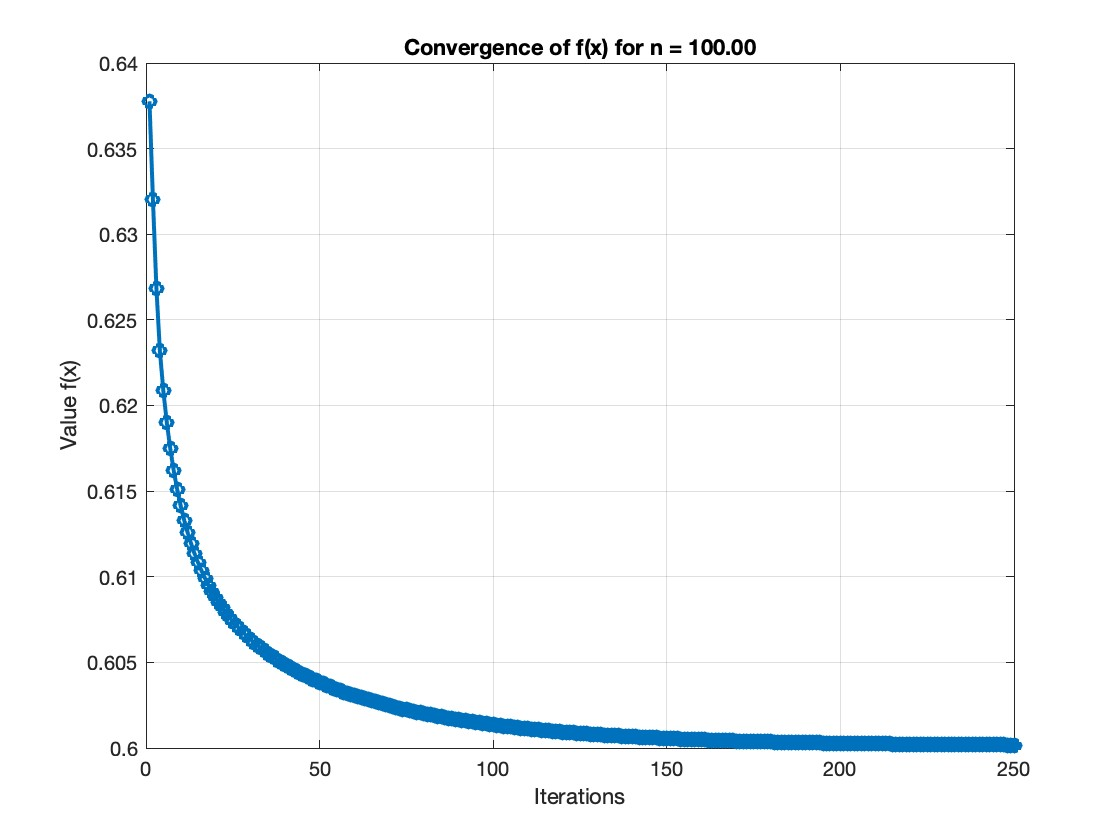
\includegraphics[width=\textwidth]{23f9.jpg}
%    \end{subfigure}
%    \begin{subfigure}[b]{0.45\textwidth}
%        \centering
%        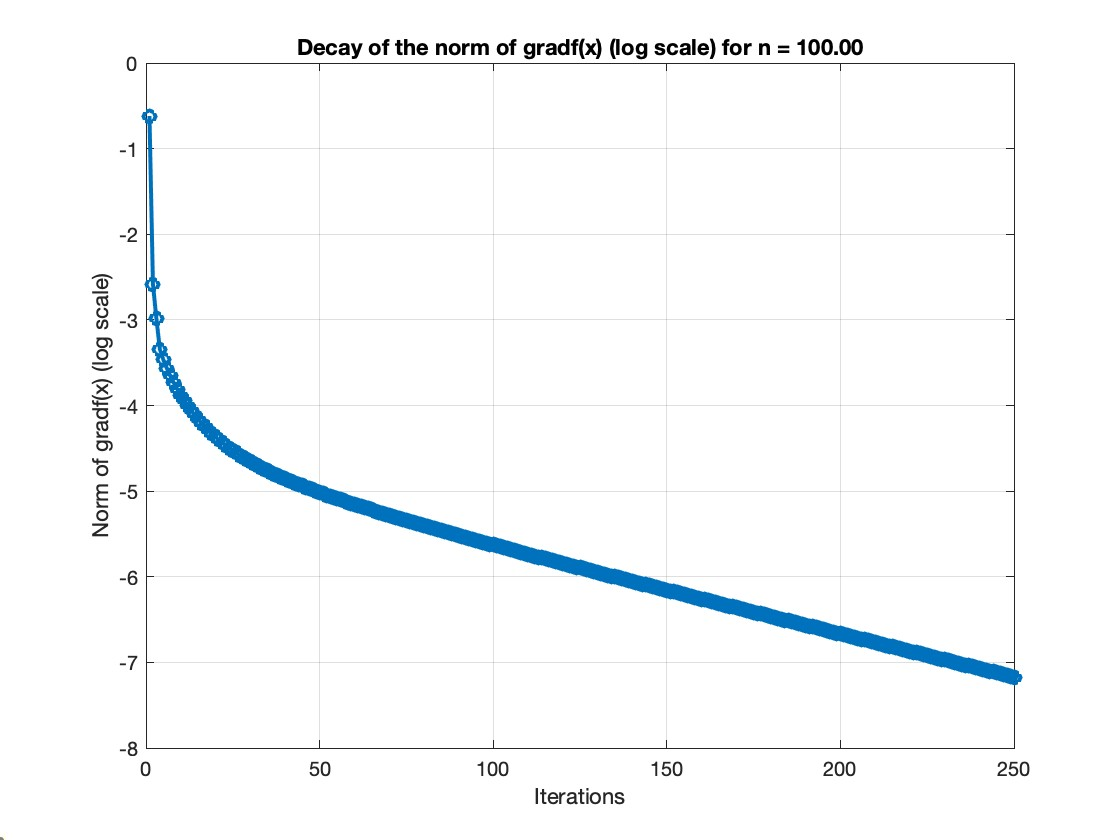
\includegraphics[width=\textwidth]{23g9.jpg}
%    \end{subfigure}
%    \caption{Experiment $9$ for $(2, 100)$}

%    \newpage

%    \begin{subfigure}[b]{0.45\textwidth}
%        \centering
%        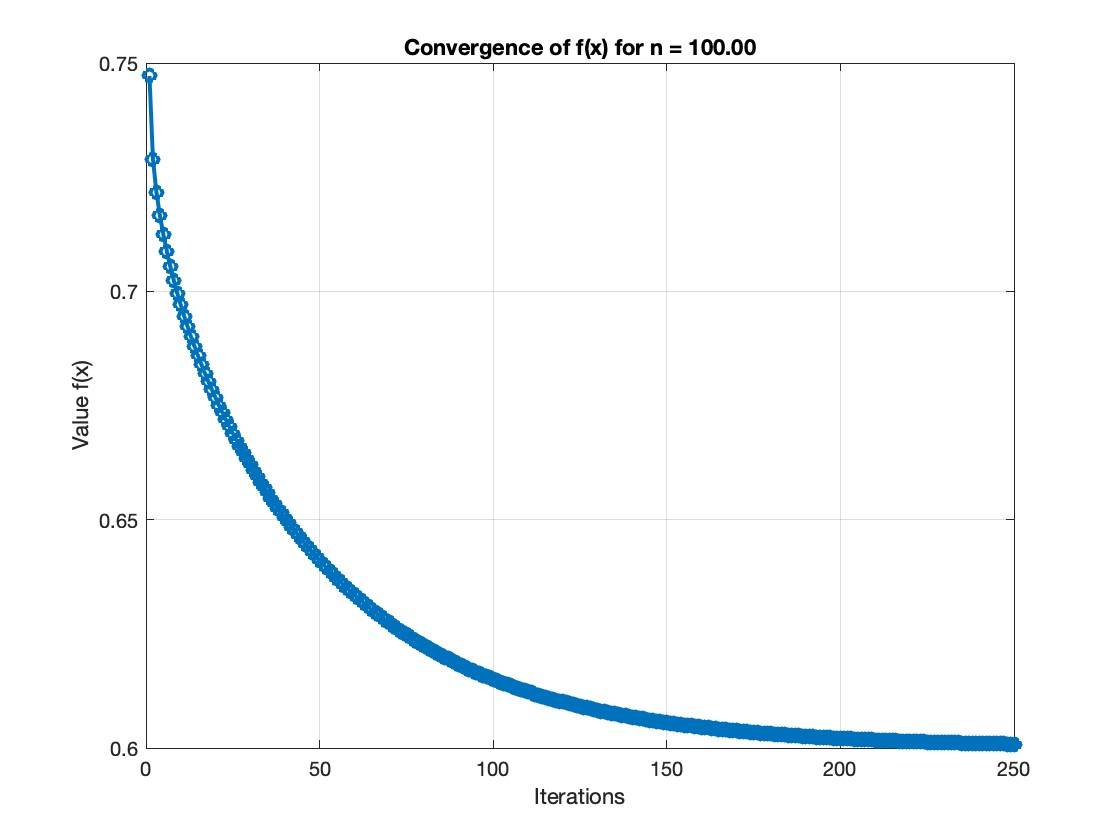
\includegraphics[width=\textwidth]{23f10.jpg}
%    \end{subfigure}
%    \begin{subfigure}[b]{0.45\textwidth}
%        \centering
%        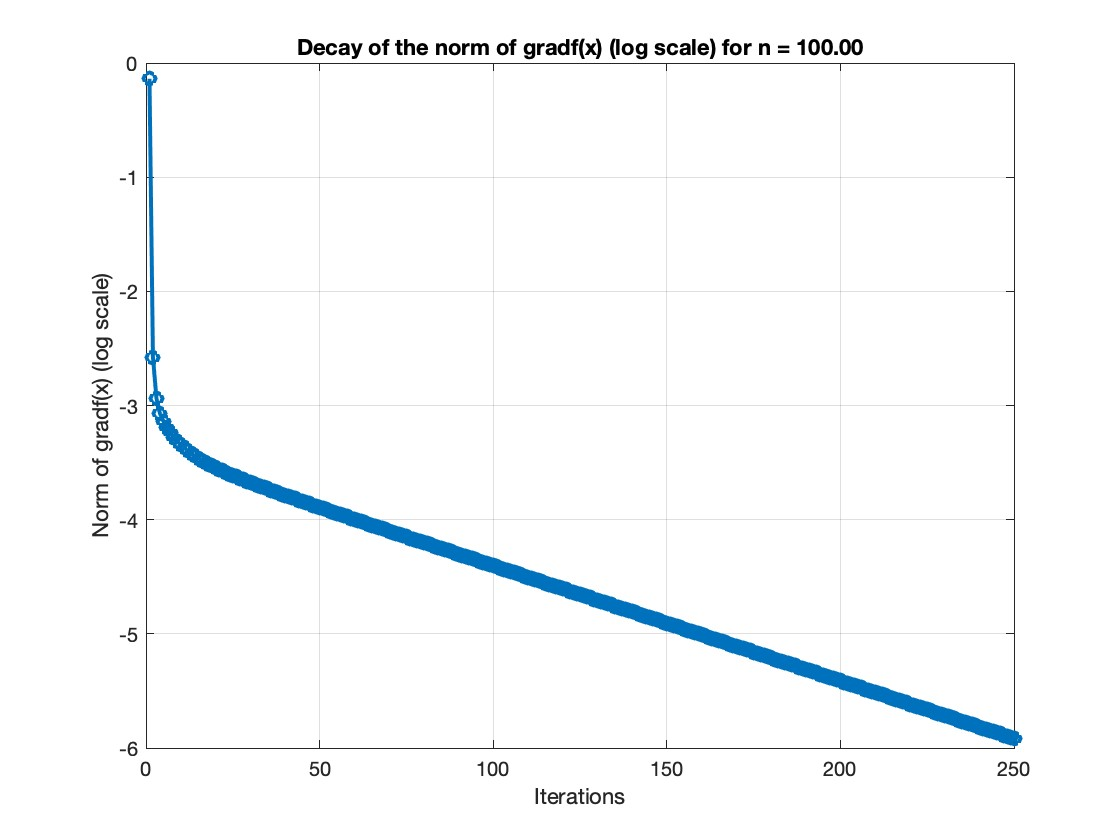
\includegraphics[width=\textwidth]{23g10.jpg}
%    \end{subfigure}
%    \caption{Experiment $10$ for $(2, 100)$}

%    \newpage

%    \begin{subfigure}[b]{0.45\textwidth}
%        \centering
%        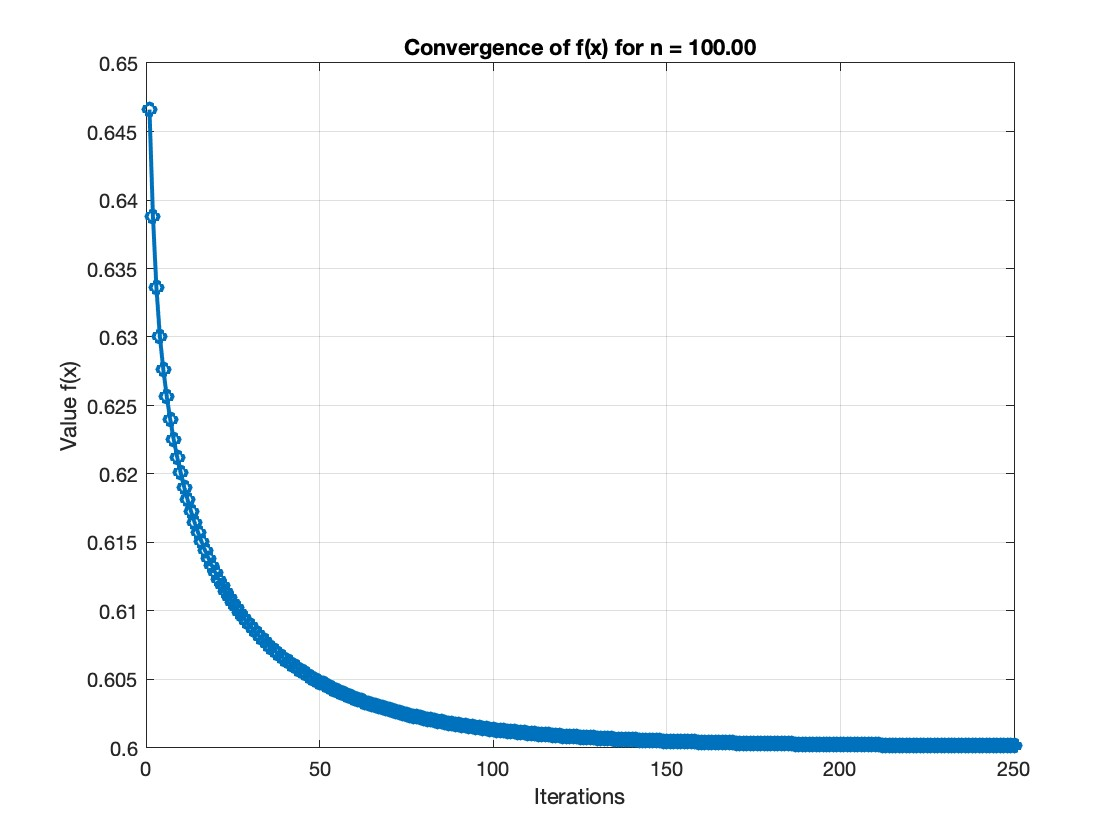
\includegraphics[width=\textwidth]{23f11.jpg}
%    \end{subfigure}
%    \begin{subfigure}[b]{0.45\textwidth}
%        \centering
%        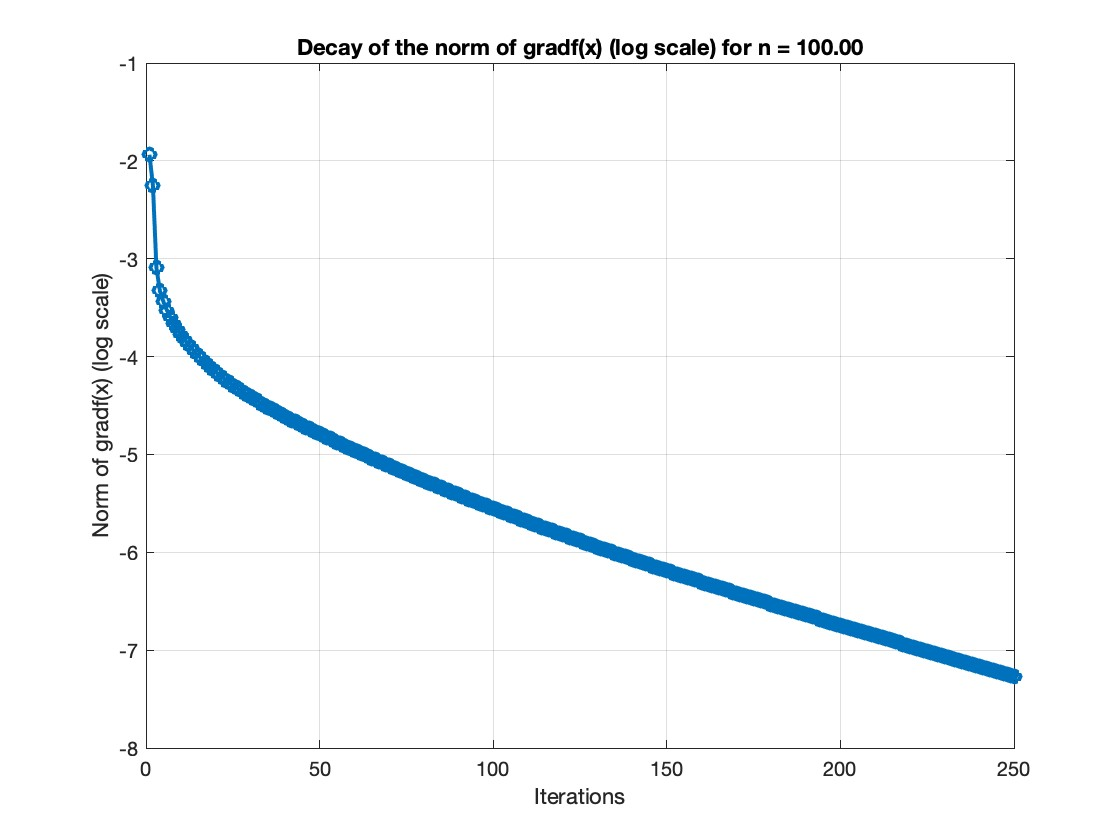
\includegraphics[width=\textwidth]{23g11.jpg}
%    \end{subfigure}
%    \caption{Experiment $11$ for $(2, 100)$}

%    \newpage

%    \begin{subfigure}[b]{0.45\textwidth}
%        \centering
%        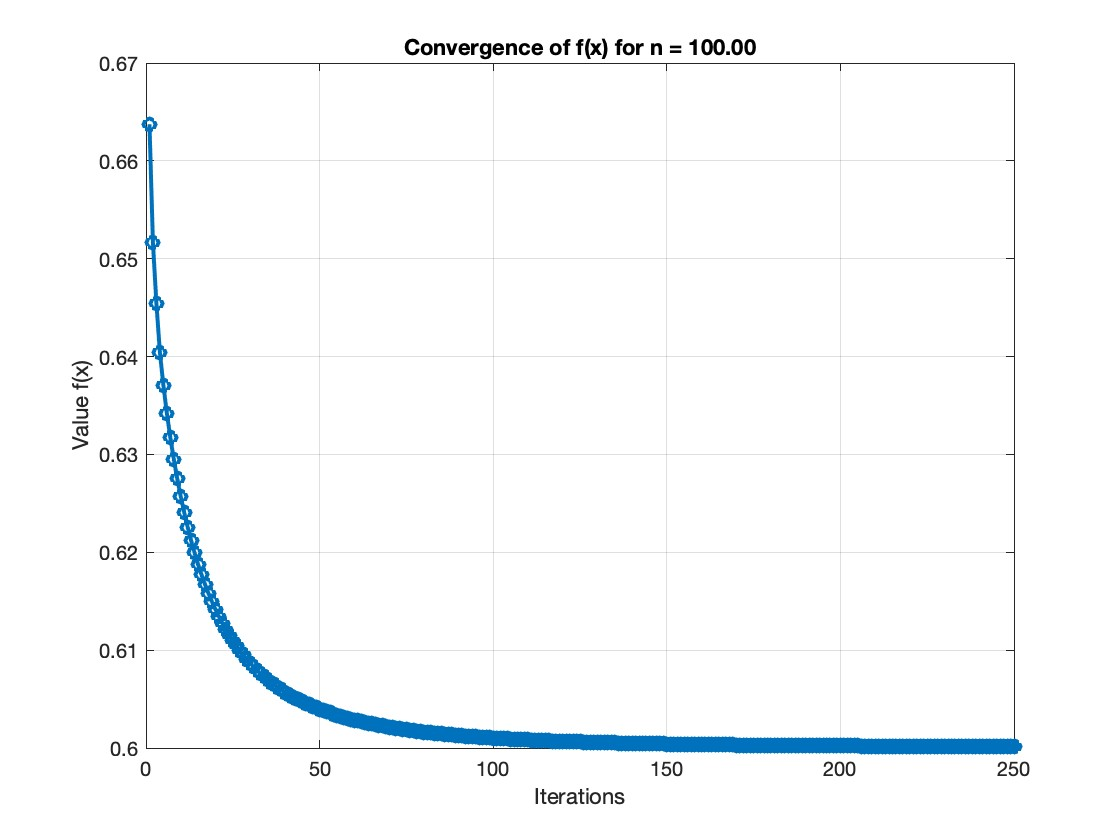
\includegraphics[width=\textwidth]{23f12.jpg}
%    \end{subfigure}
%    \begin{subfigure}[b]{0.45\textwidth}
%        \centering
%        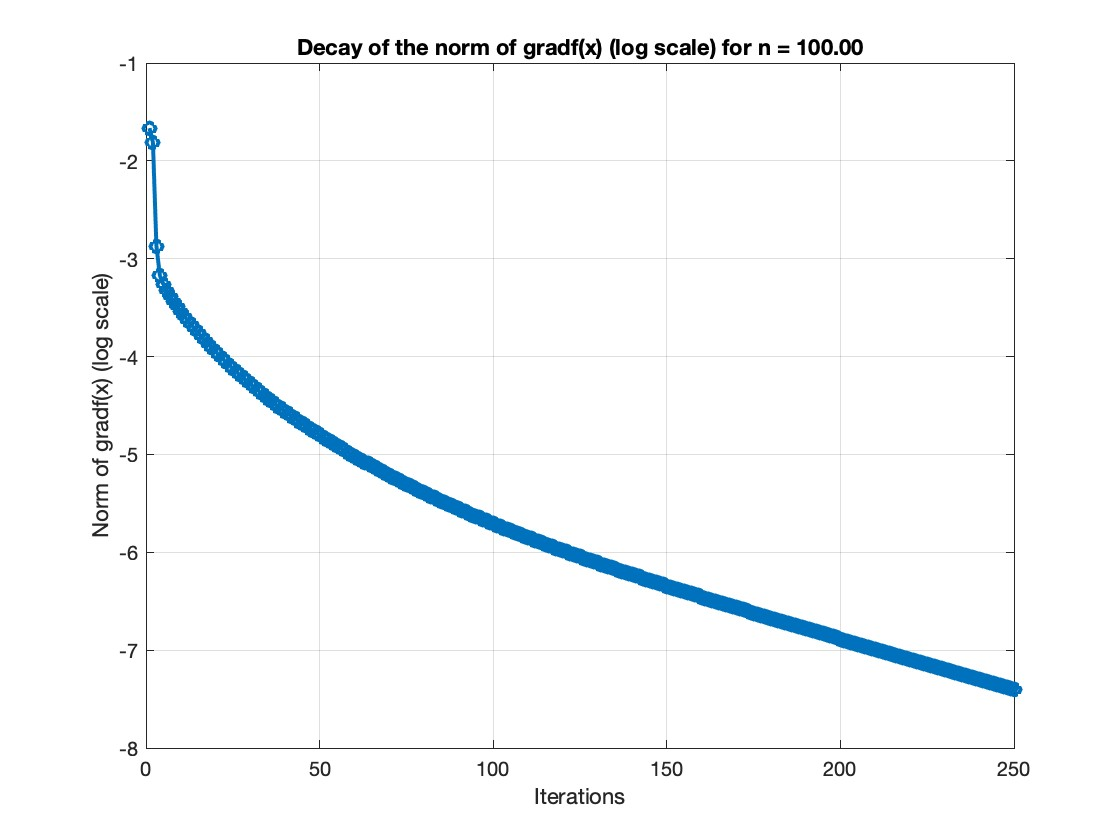
\includegraphics[width=\textwidth]{23g12.jpg}
%    \end{subfigure}
%    \caption{Experiment $12$ for $(2, 100)$}
%\end{figure}
\begin{figure}[H]
    \centering
    %\begin{subfigure}[b]{0.45\textwidth}
    %    \centering
    %    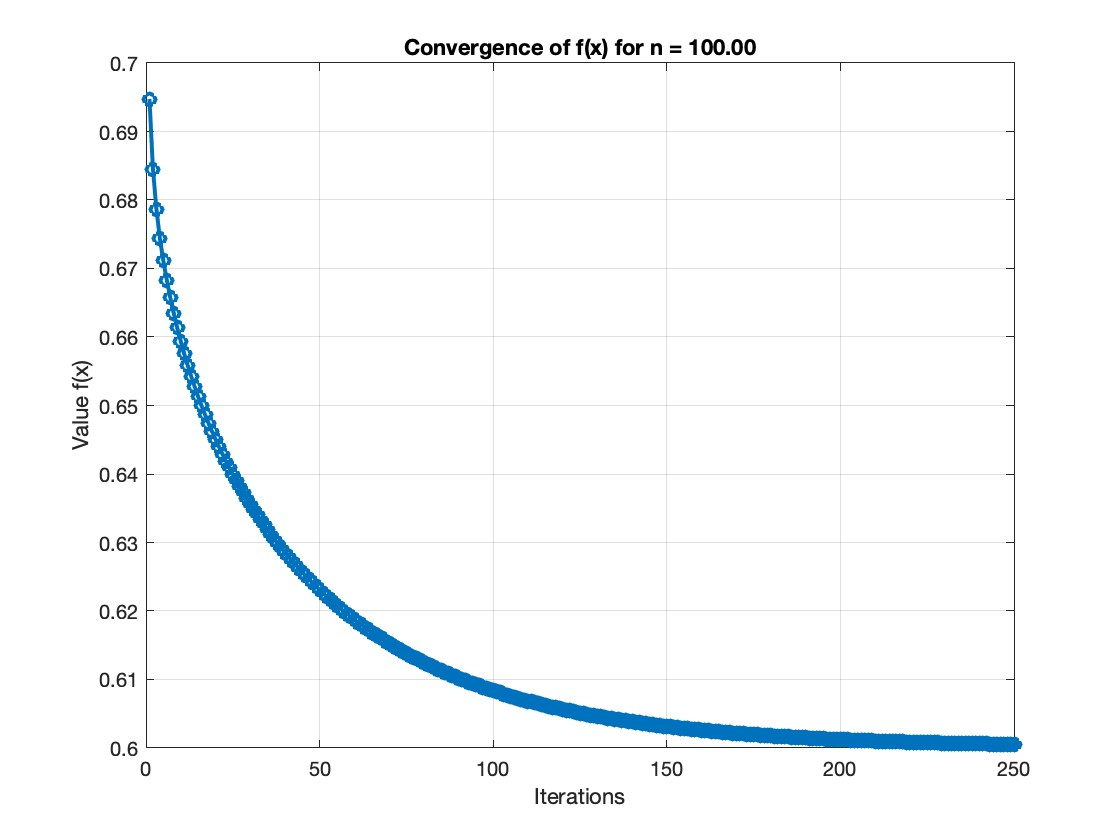
\includegraphics[width=\textwidth]{23f13.jpg}
    %\end{subfigure}
    %\begin{subfigure}[b]{0.45\textwidth}
    %    \centering
    %    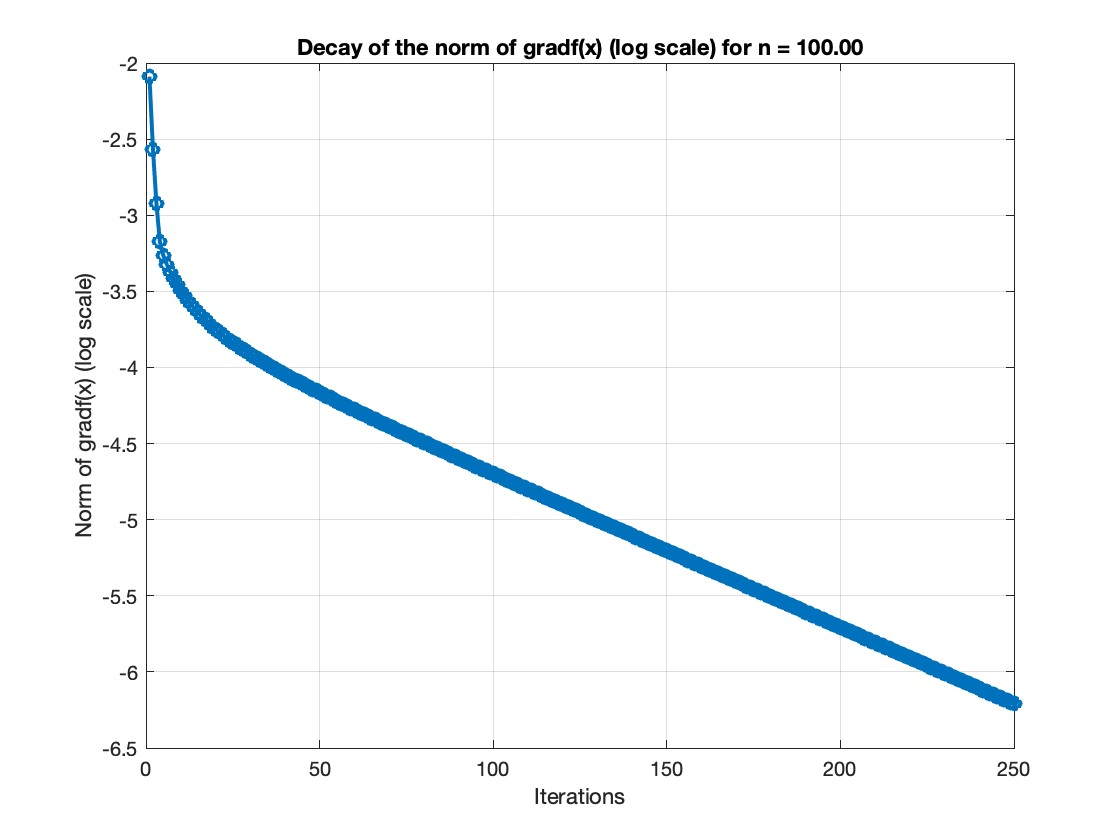
\includegraphics[width=\textwidth]{23g13.jpg}
    %\end{subfigure}
    %\caption{Experiment $13$ for $(2, 100)$}

    %\newpage

    %\begin{subfigure}[b]{0.45\textwidth}
    %    \centering
    %    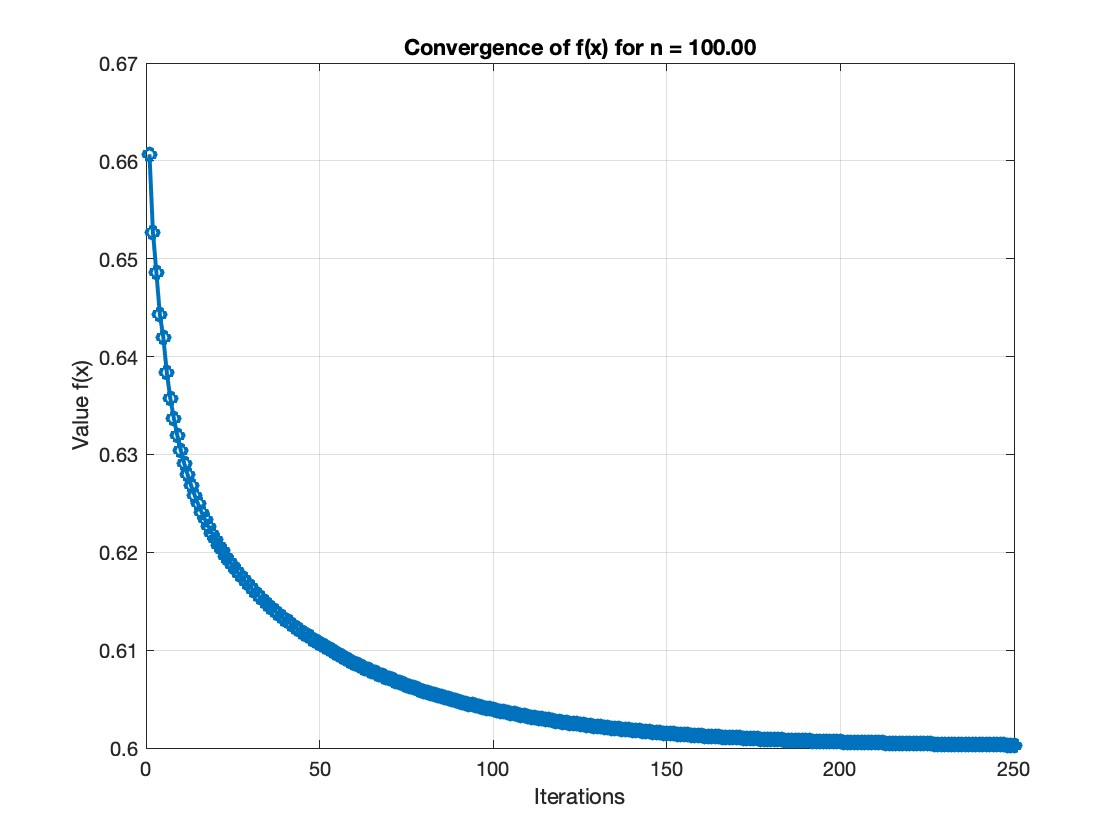
\includegraphics[width=\textwidth]{23f14.jpg}
    %\end{subfigure}
    %\begin{subfigure}[b]{0.45\textwidth}
    %    \centering
    %    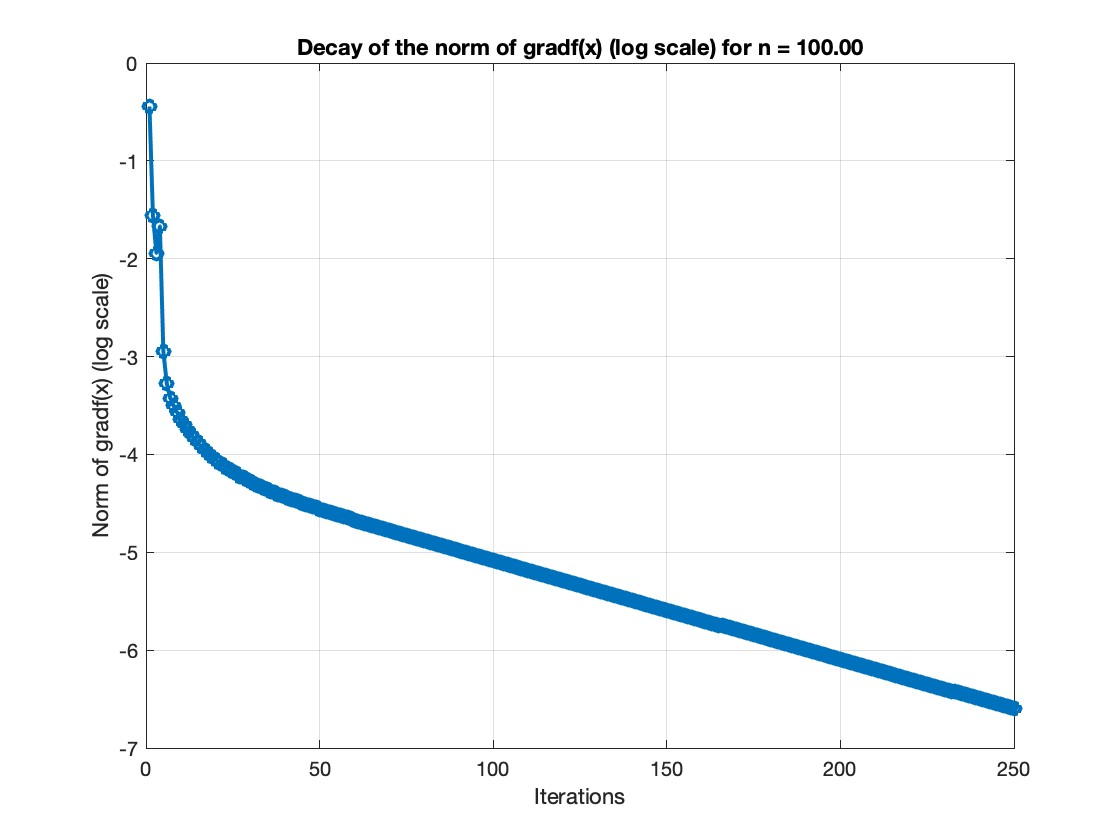
\includegraphics[width=\textwidth]{23g14.jpg}
    %\end{subfigure}
    %\caption{Experiment $14$ for $(2, 100)$}

    %\newpage

    \begin{subfigure}[b]{0.49\textwidth}
        \centering
        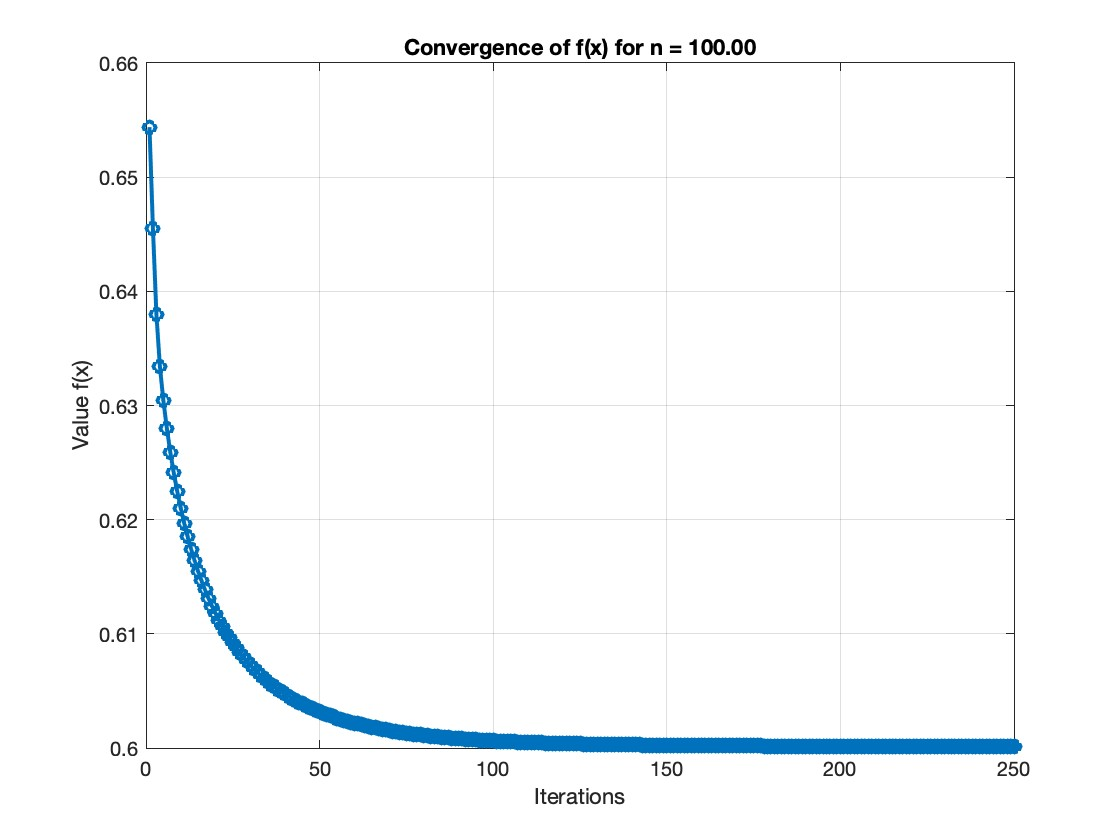
\includegraphics[width=\textwidth]{23f15.jpg}
    \end{subfigure}
    \begin{subfigure}[b]{0.49\textwidth}
        \centering
        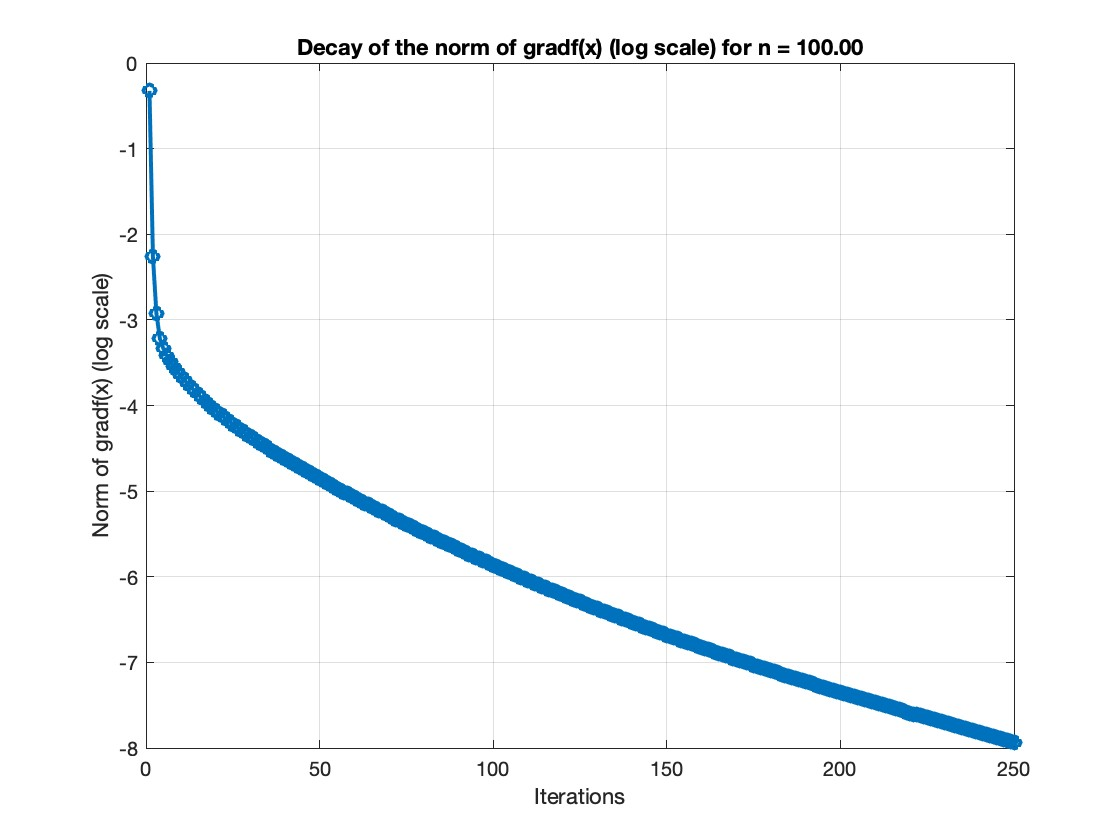
\includegraphics[width=\textwidth]{23g15.jpg}
    \end{subfigure}
    \caption{Experiment $15$ for $(2, 100)$, corresponding to the best configuration obtained}
    \label{fig:2315}

    %\newpage

    %\begin{subfigure}[b]{0.45\textwidth}
    %    \centering
    %    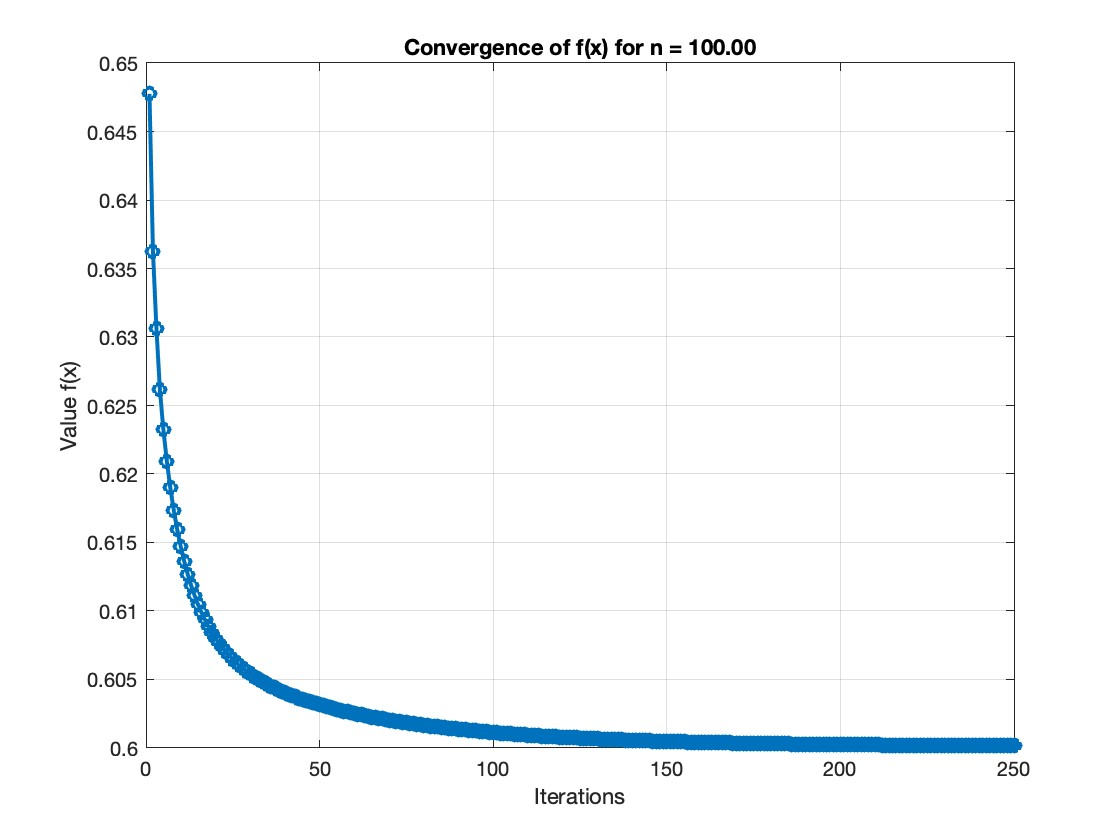
\includegraphics[width=\textwidth]{23f16.jpg}
    %\end{subfigure}
    %\begin{subfigure}[b]{0.45\textwidth}
    %    \centering
    %    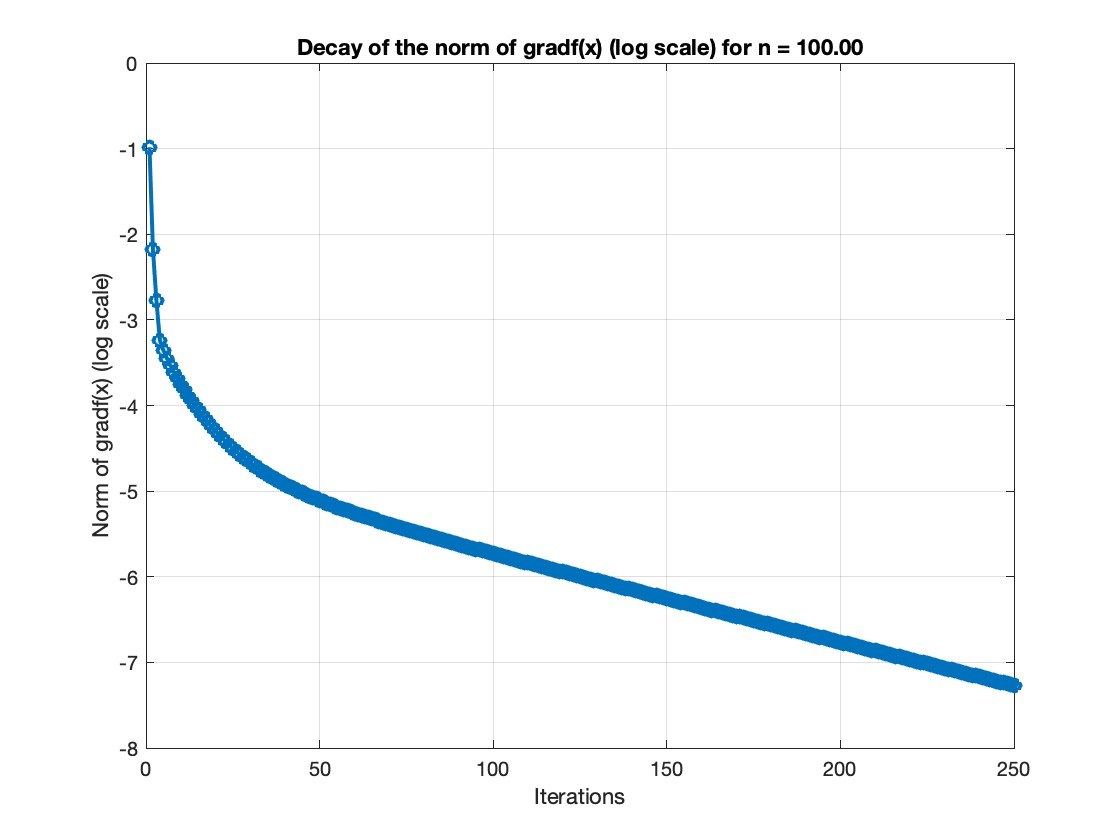
\includegraphics[width=\textwidth]{23g16.jpg}
    %\end{subfigure}
    %\caption{Experiment $16$ for $(2, 100)$}
\end{figure}
%\begin{figure}
%    \centering
%    \begin{subfigure}[b]{0.45\textwidth}
%        \centering
%        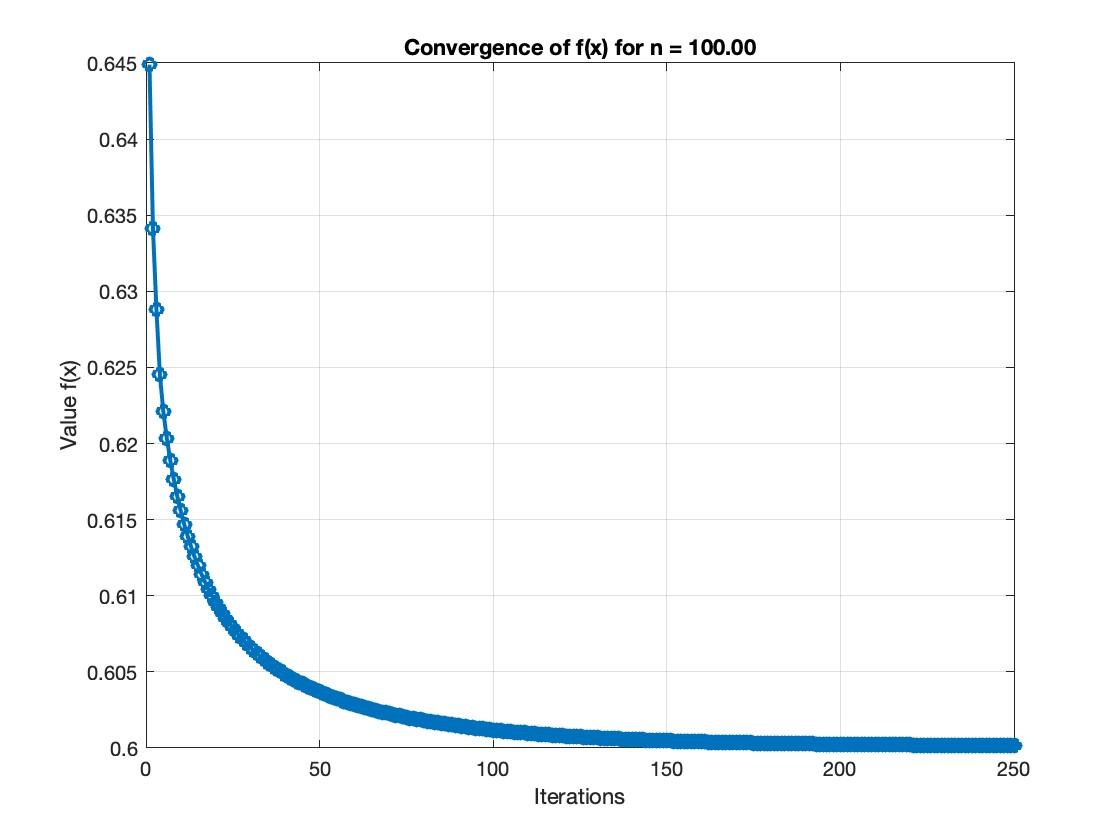
\includegraphics[width=\textwidth]{23f17.jpg}
%    \end{subfigure}
%    \begin{subfigure}[b]{0.45\textwidth}
%        \centering
%        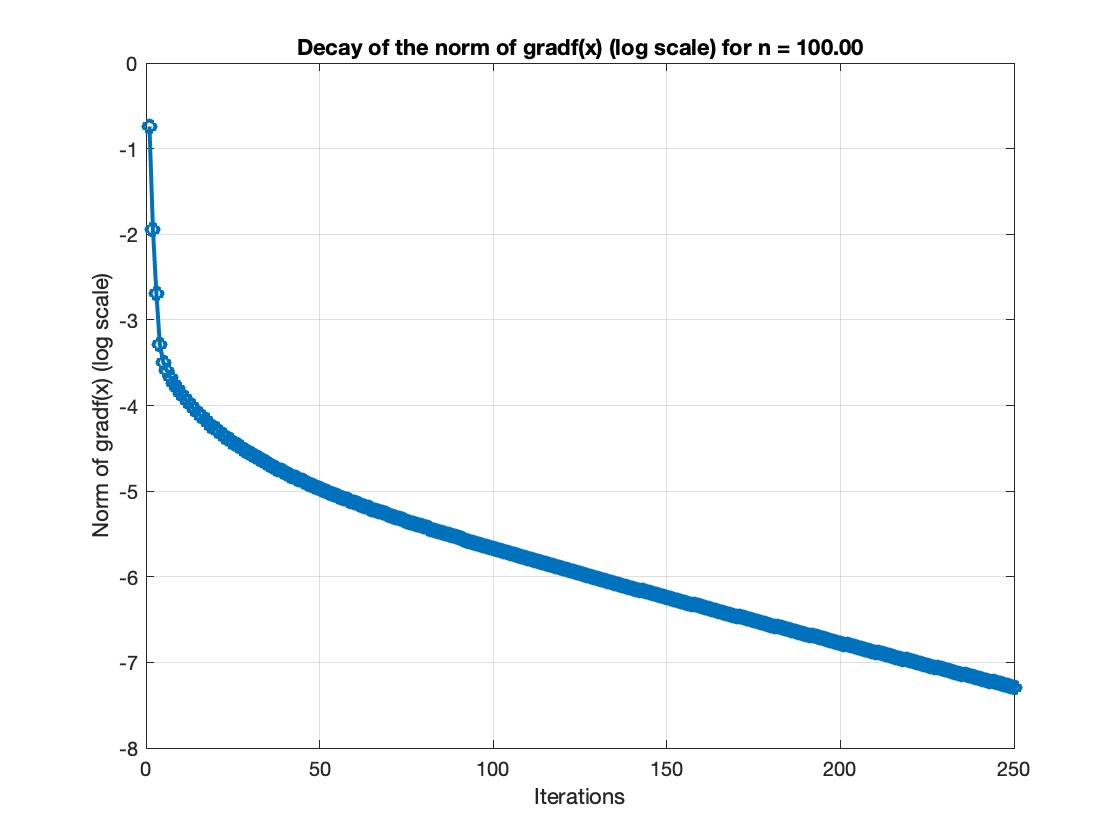
\includegraphics[width=\textwidth]{23g17.jpg}
%    \end{subfigure}
%    \caption{Experiment $17$ for $(2, 100)$}

%    \newpage

%    \begin{subfigure}[b]{0.45\textwidth}
%        \centering
%        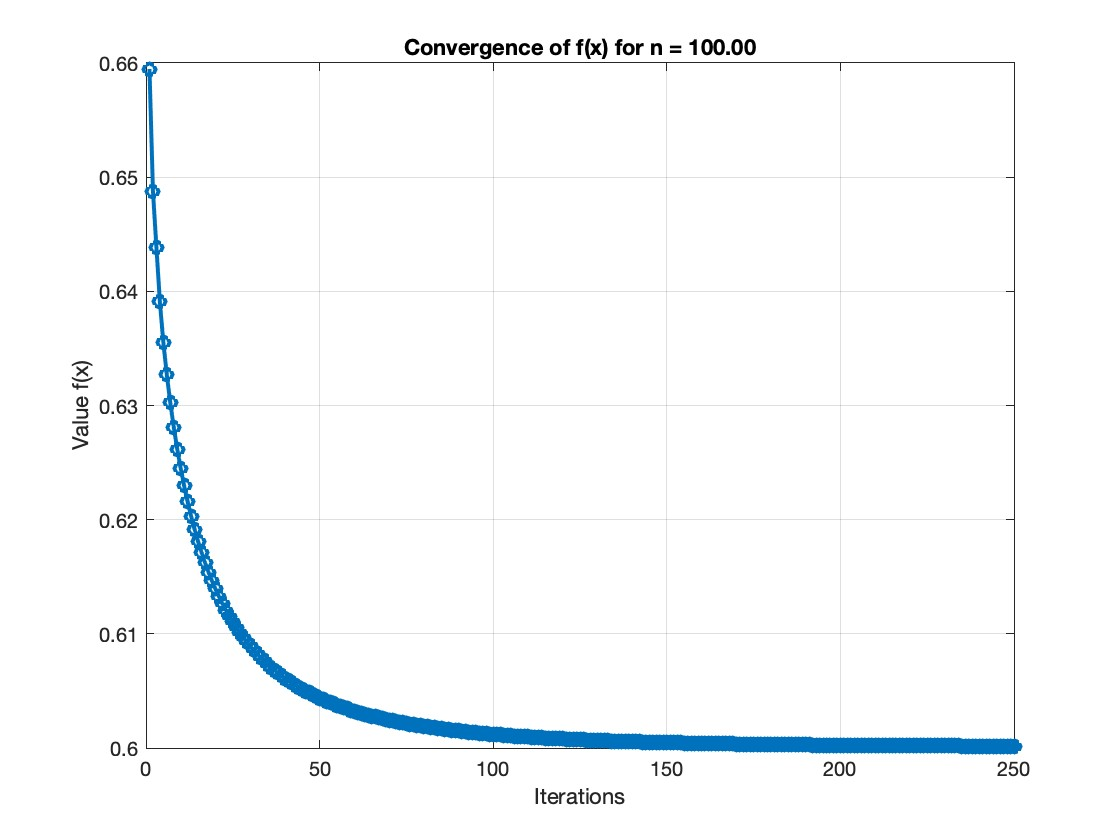
\includegraphics[width=\textwidth]{23f18.jpg}
%    \end{subfigure}
%    \begin{subfigure}[b]{0.45\textwidth}
%        \centering
%        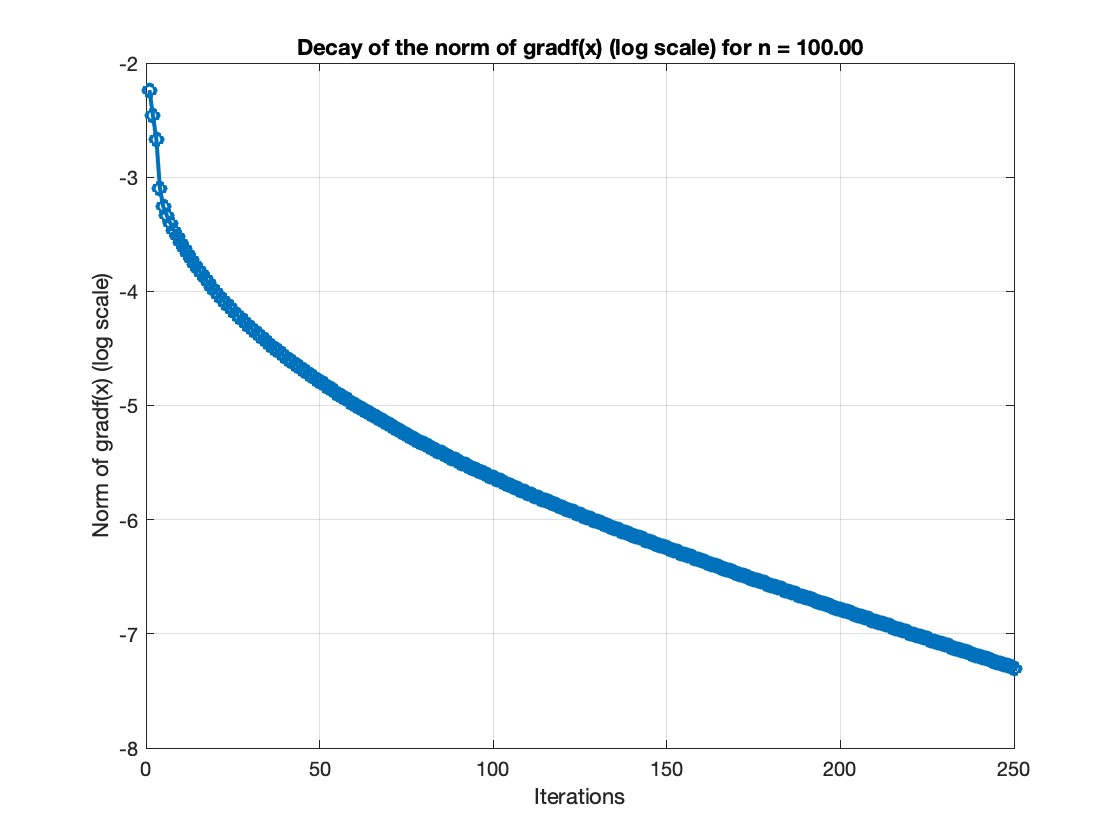
\includegraphics[width=\textwidth]{23g18.jpg}
%    \end{subfigure}
%    \caption{Experiment $18$ for $(2, 100)$}

%    \newpage

%    \begin{subfigure}[b]{0.45\textwidth}
%        \centering
%        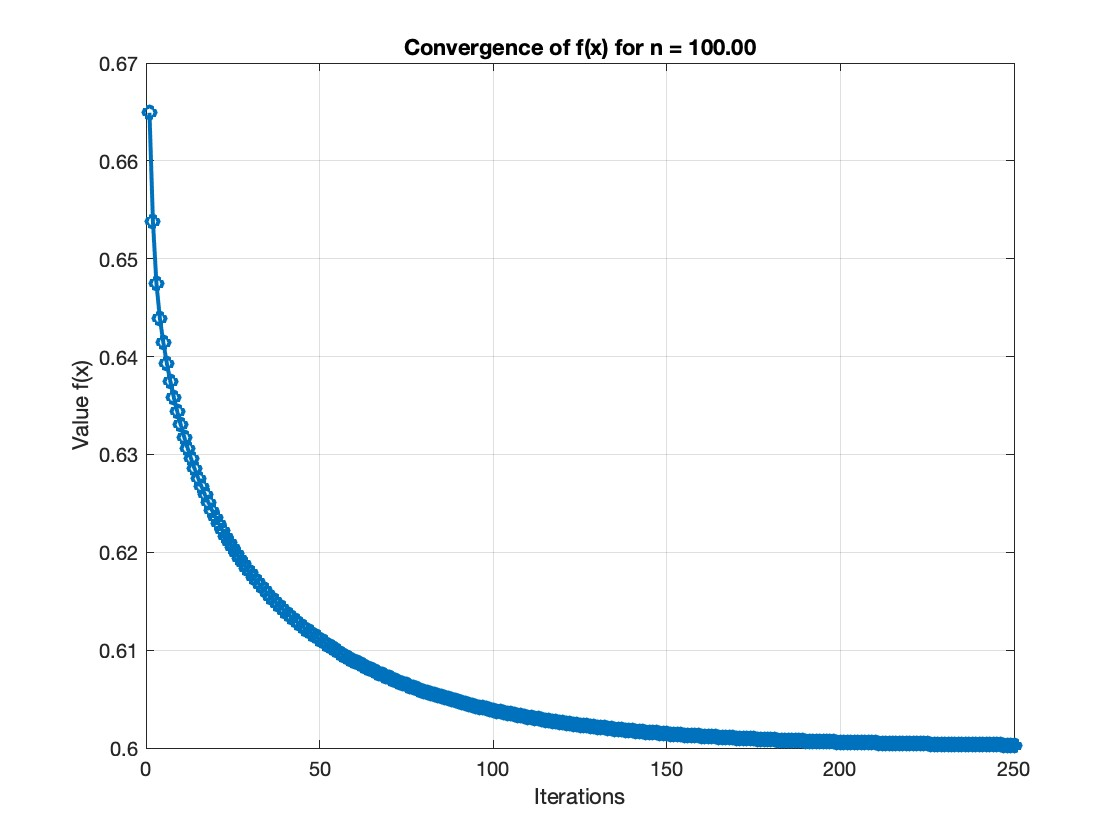
\includegraphics[width=\textwidth]{23f19.jpg}
%    \end{subfigure}
%    \begin{subfigure}[b]{0.45\textwidth}
%        \centering
%        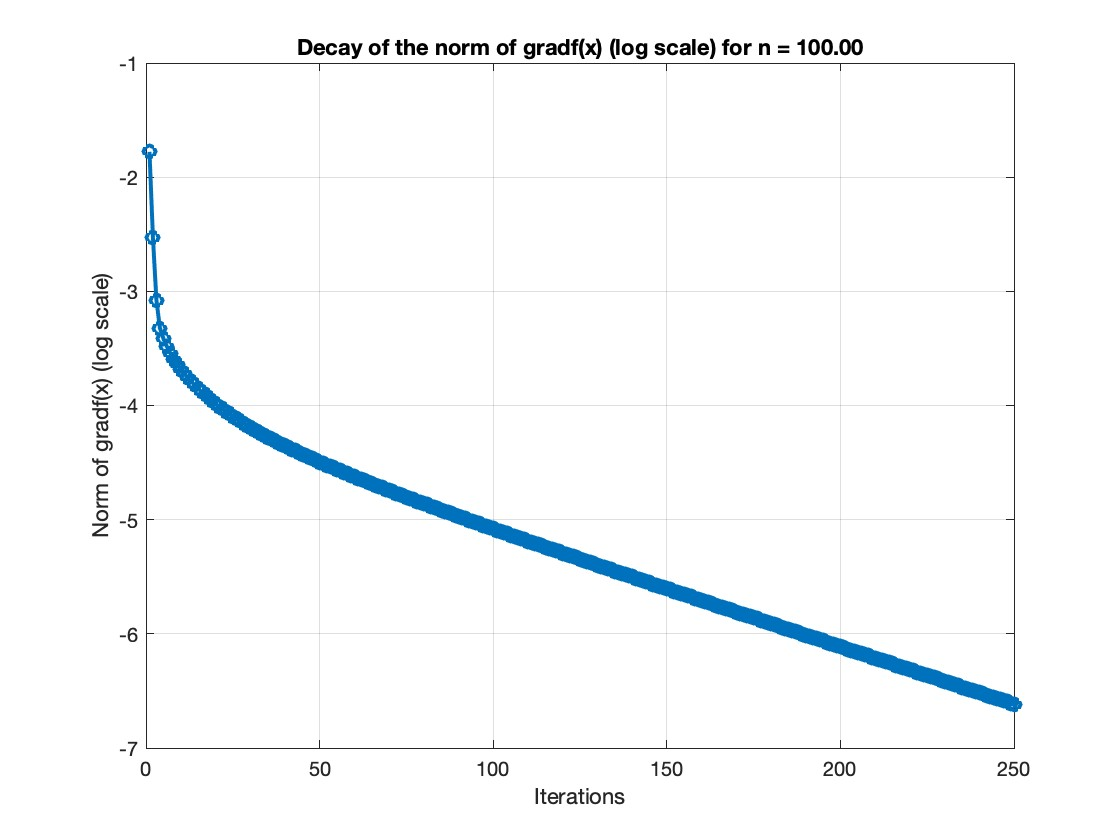
\includegraphics[width=\textwidth]{23g19.jpg}
%    \end{subfigure}
%    \caption{Experiment $19$ for $(2, 100)$}

%    \newpage

%    \begin{subfigure}[b]{0.45\textwidth}
%        \centering
%        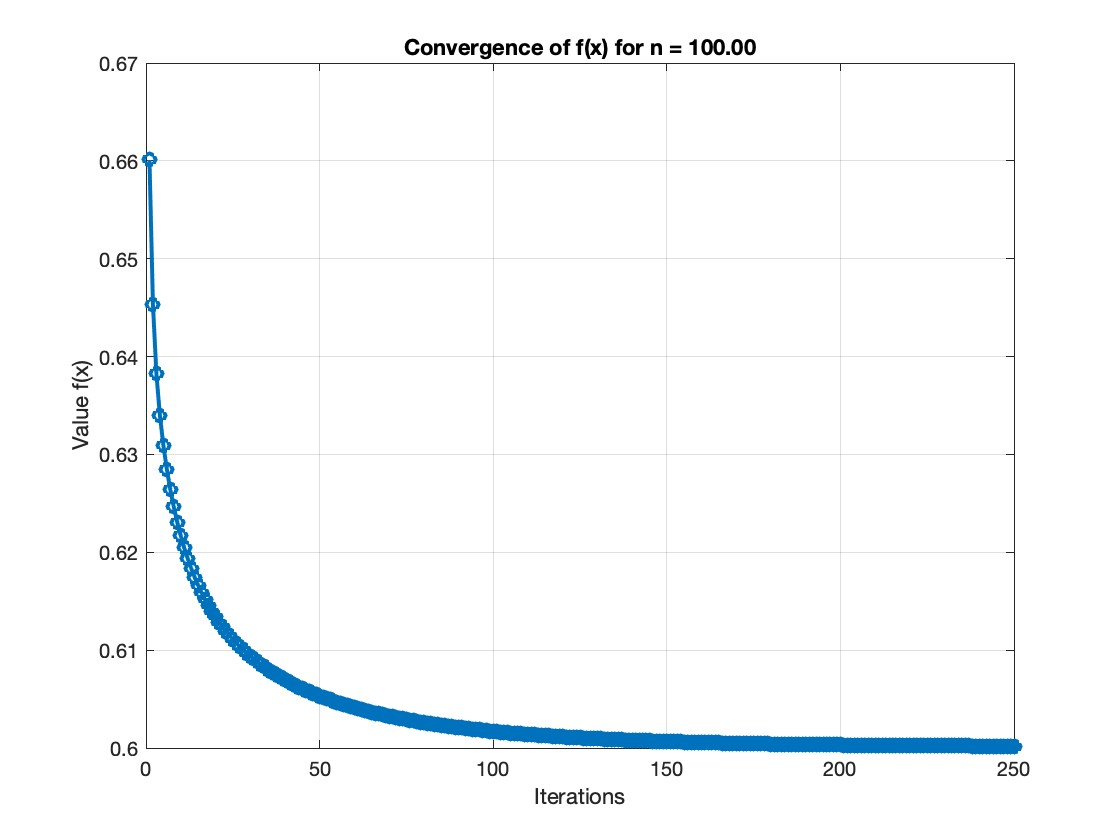
\includegraphics[width=\textwidth]{23f20.jpg}
%    \end{subfigure}
%    \begin{subfigure}[b]{0.45\textwidth}
%        \centering
%        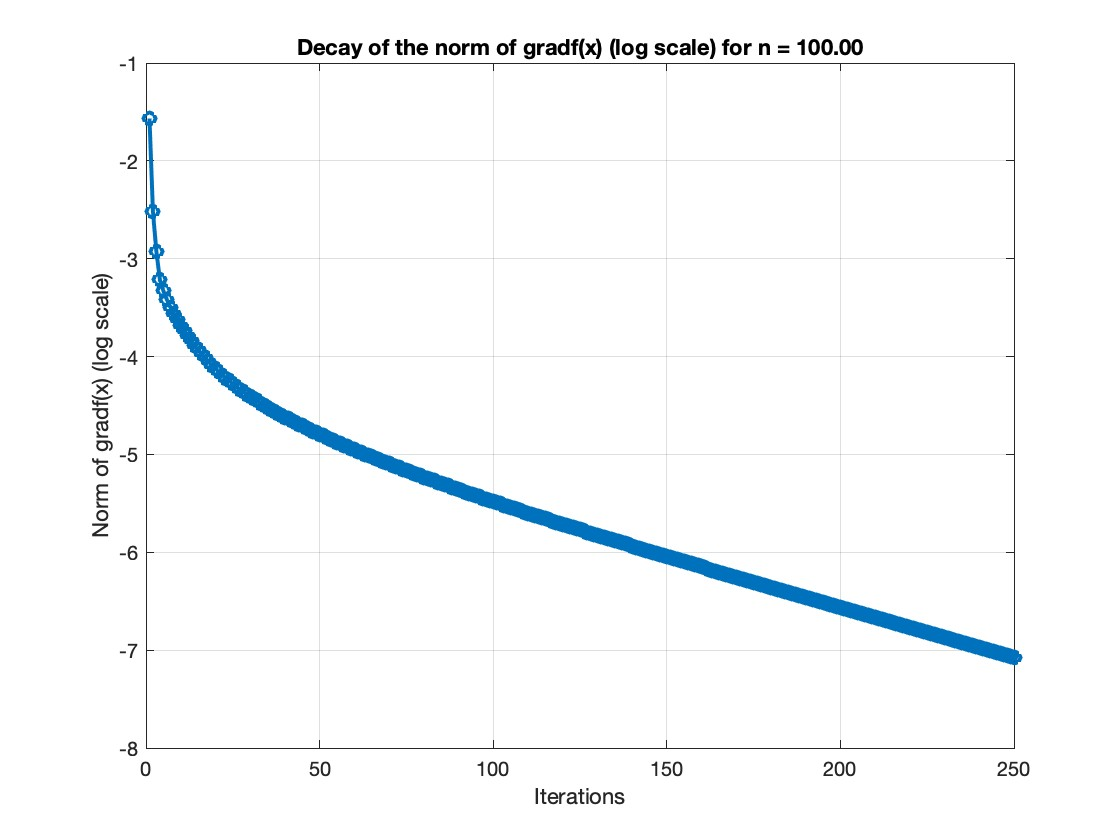
\includegraphics[width=\textwidth]{23g20.jpg}
%    \end{subfigure}
%    \caption{Experiment $20$ for $(2, 100)$}
%\end{figure}
%\begin{figure}
%    \centering
%    \begin{subfigure}[b]{0.45\textwidth}
%        \centering
%        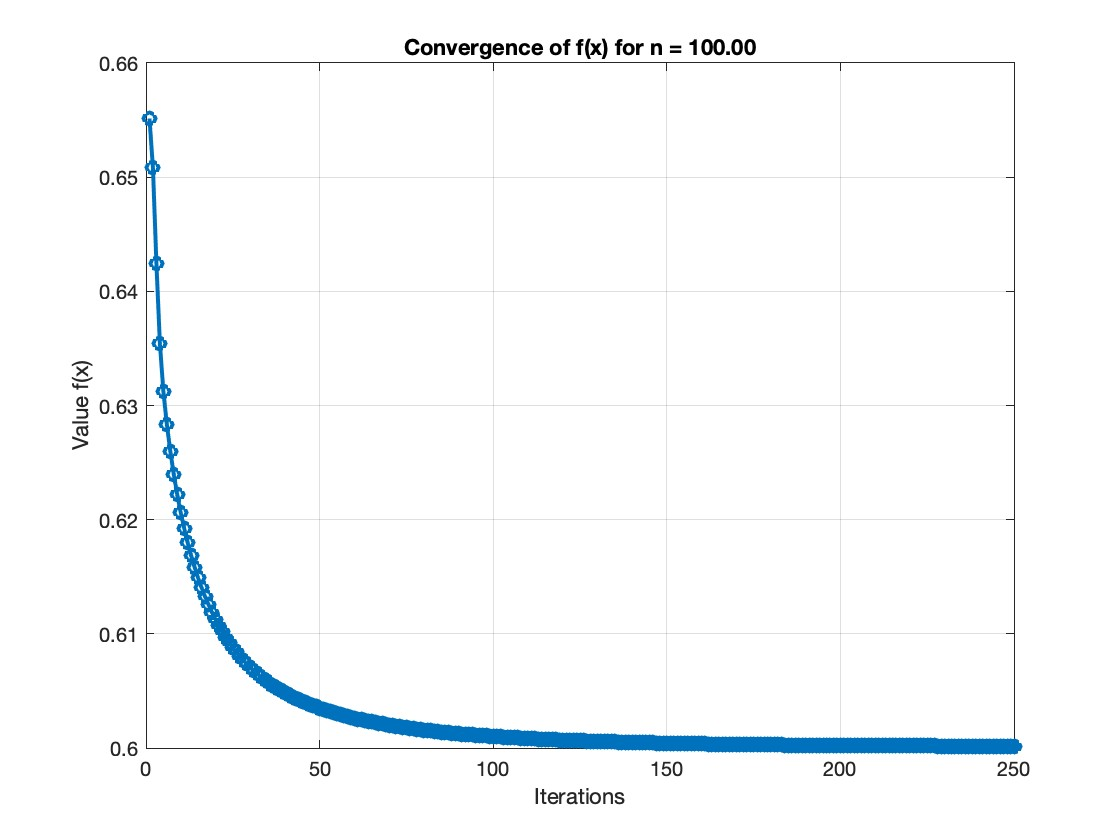
\includegraphics[width=\textwidth]{23f21.jpg}
%    \end{subfigure}
%    \begin{subfigure}[b]{0.45\textwidth}
%        \centering
%        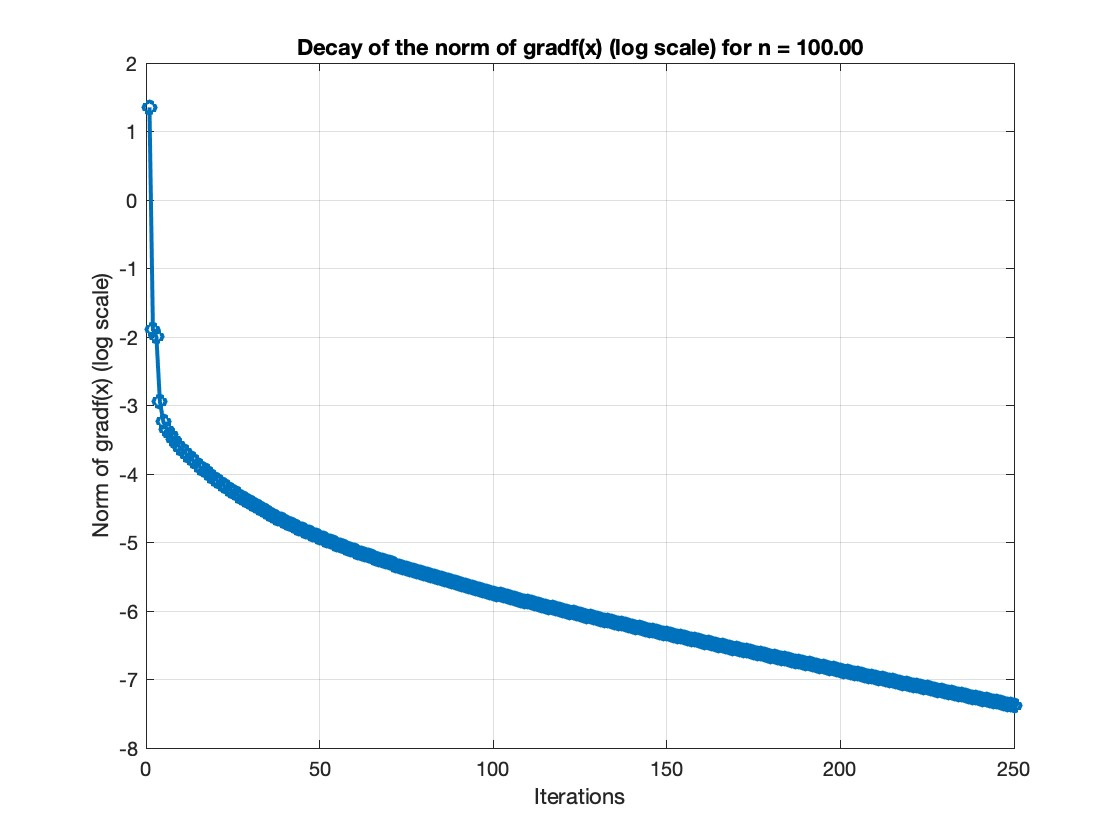
\includegraphics[width=\textwidth]{23g21.jpg}
%    \end{subfigure}
%    \caption{Experiment $21$ for $(2, 100)$}

%    \newpage

%    \begin{subfigure}[b]{0.45\textwidth}
%        \centering
%        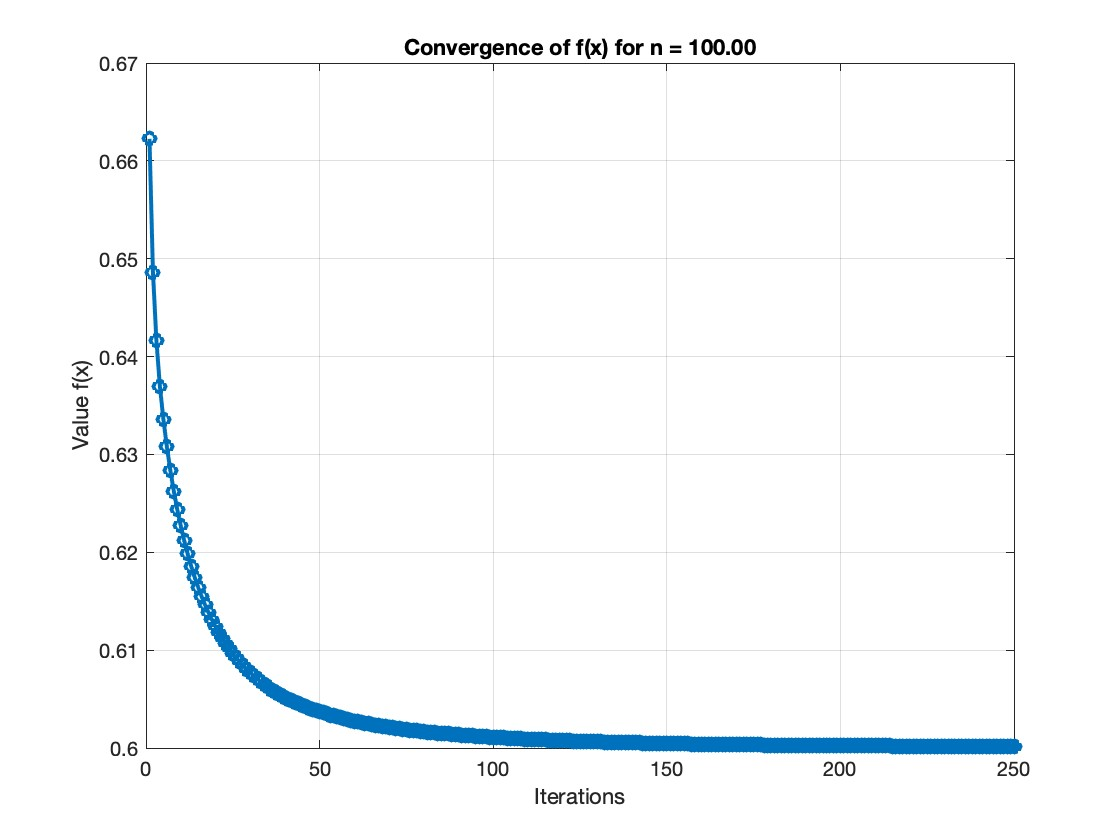
\includegraphics[width=\textwidth]{23f22.jpg}
%    \end{subfigure}
%    \begin{subfigure}[b]{0.45\textwidth}
%        \centering
%        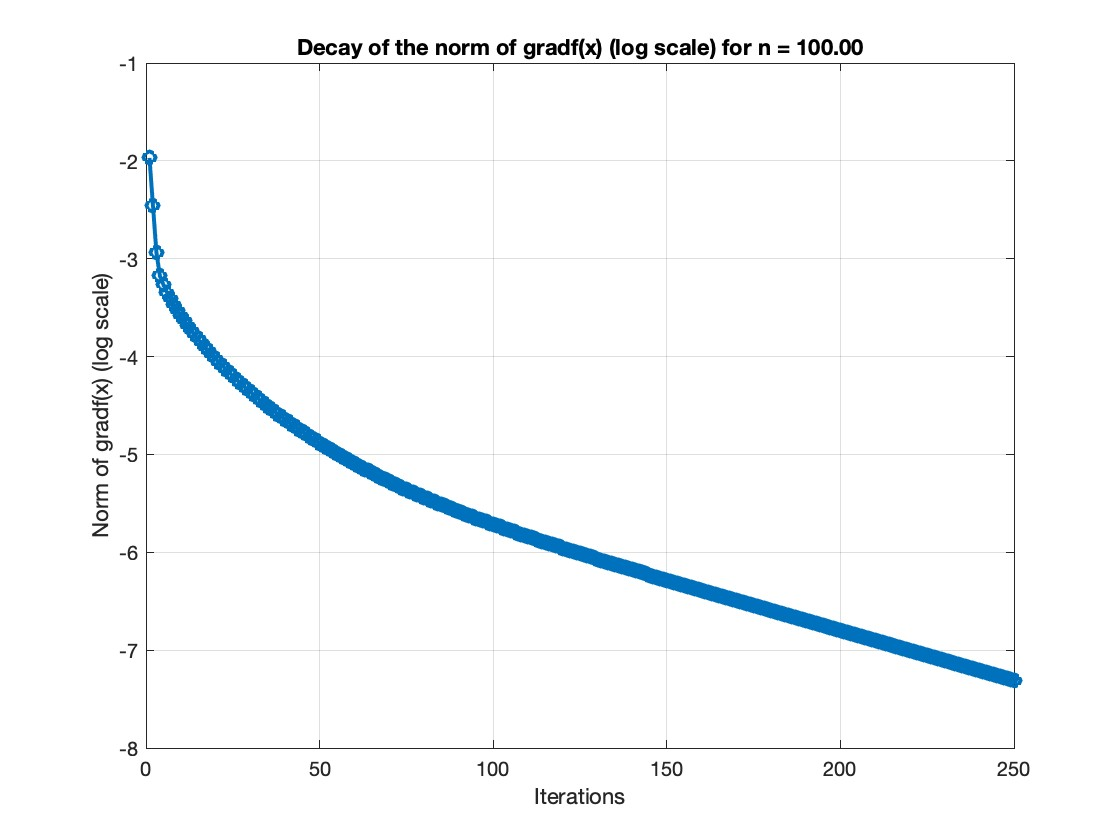
\includegraphics[width=\textwidth]{23g22.jpg}
%    \end{subfigure}
%    \caption{Experiment $22$ for $(2, 100)$}

%    \newpage

%    \begin{subfigure}[b]{0.45\textwidth}
%        \centering
%        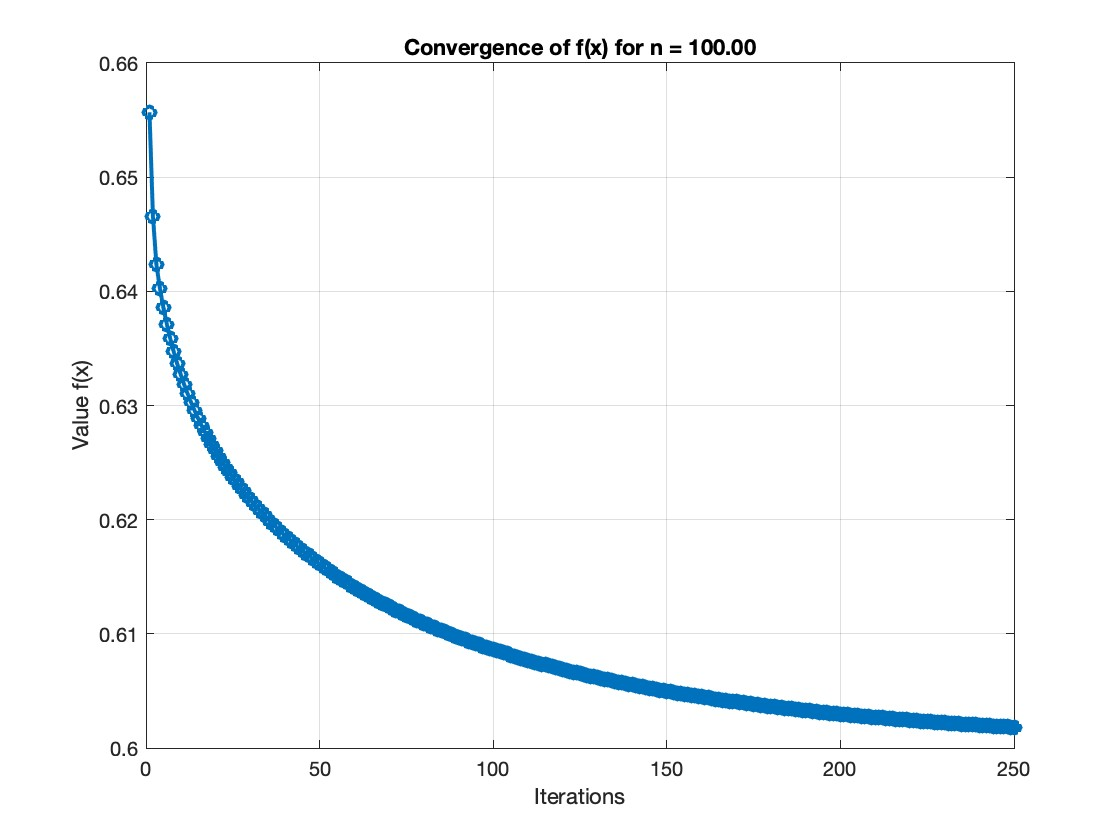
\includegraphics[width=\textwidth]{23f23.jpg}
%    \end{subfigure}
%    \begin{subfigure}[b]{0.45\textwidth}
%        \centering
%        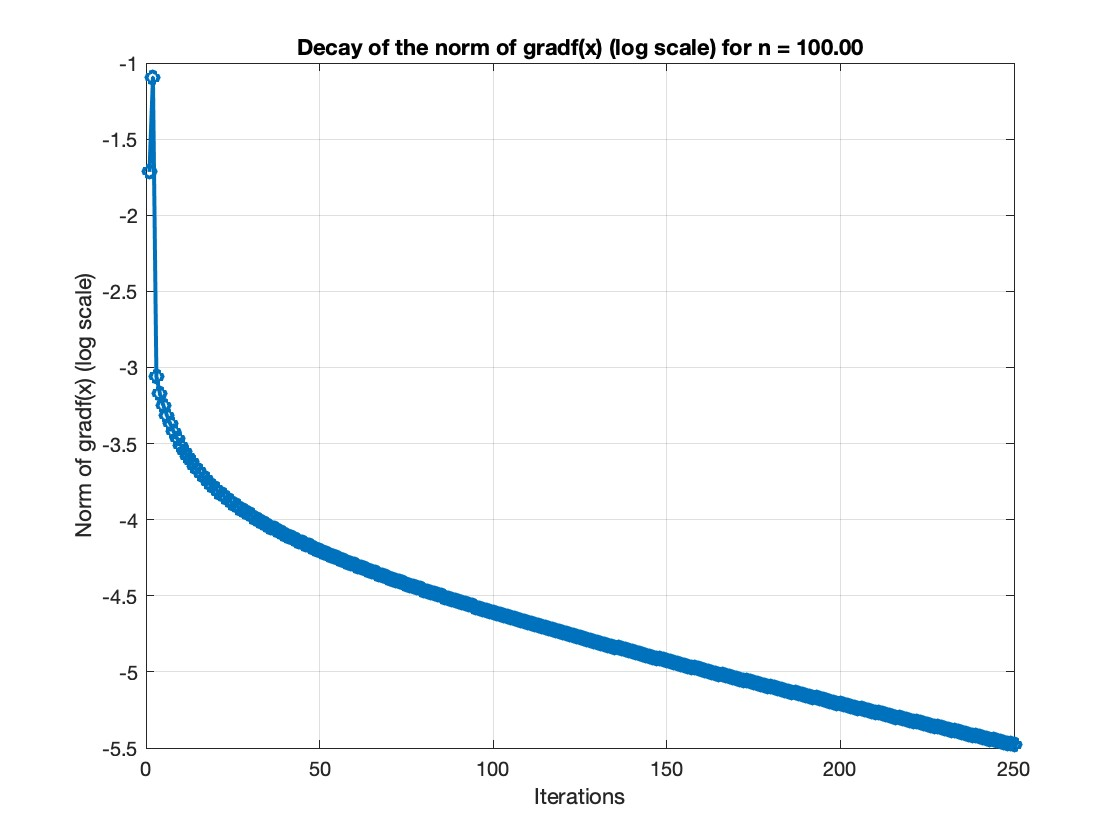
\includegraphics[width=\textwidth]{23g23.jpg}
%    \end{subfigure}
%    \caption{Experiment $23$ for $(2, 100)$}

%    \newpage

%    \begin{subfigure}[b]{0.45\textwidth}
%        \centering
%        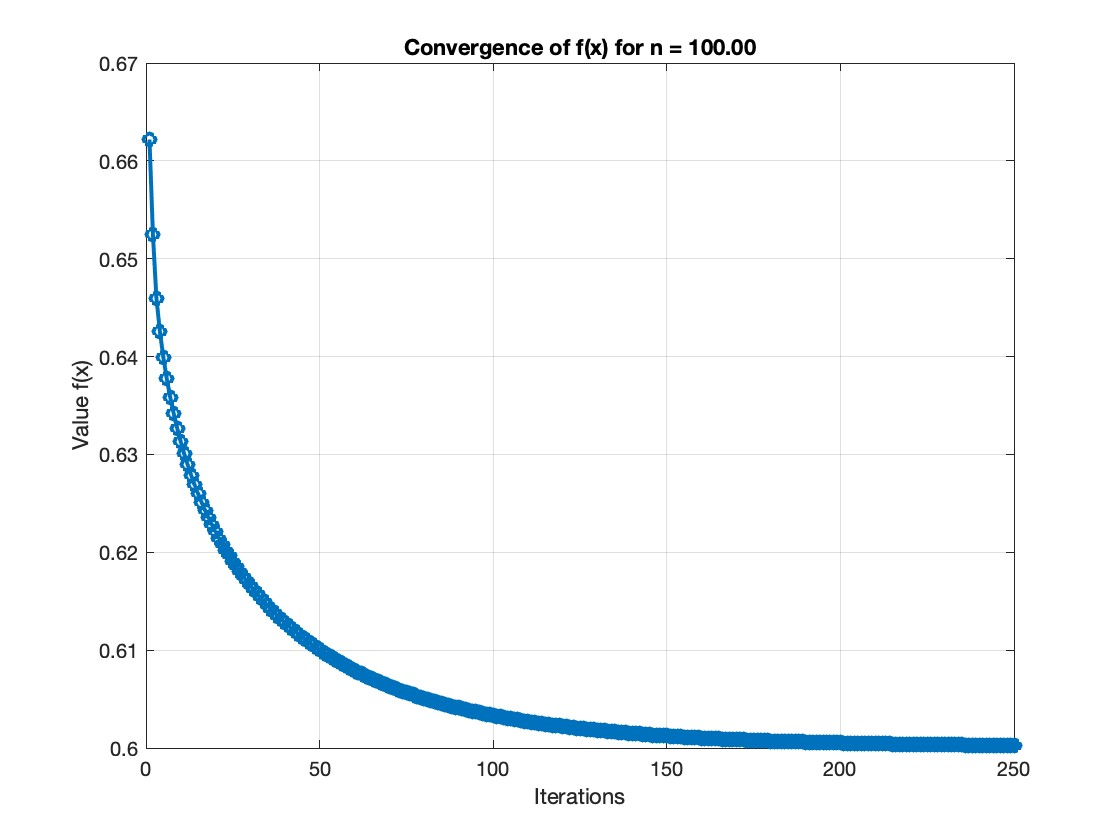
\includegraphics[width=\textwidth]{23f24.jpg}
%    \end{subfigure}
%    \begin{subfigure}[b]{0.45\textwidth}
%        \centering
%        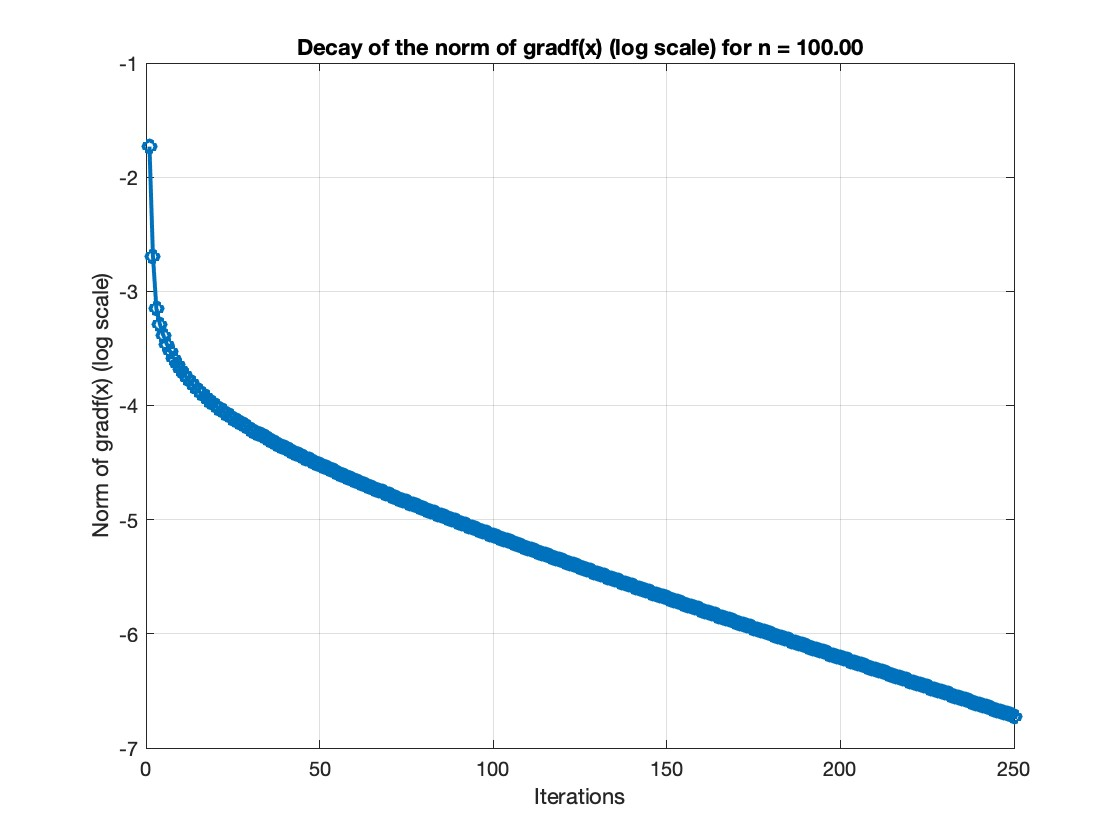
\includegraphics[width=\textwidth]{23g24.jpg}
%    \end{subfigure}
%    \caption{Experiment $24$ for $(2, 100)$}
%\end{figure}
%\begin{figure}
%    \centering
%    \begin{subfigure}[b]{0.45\textwidth}
%        \centering
%        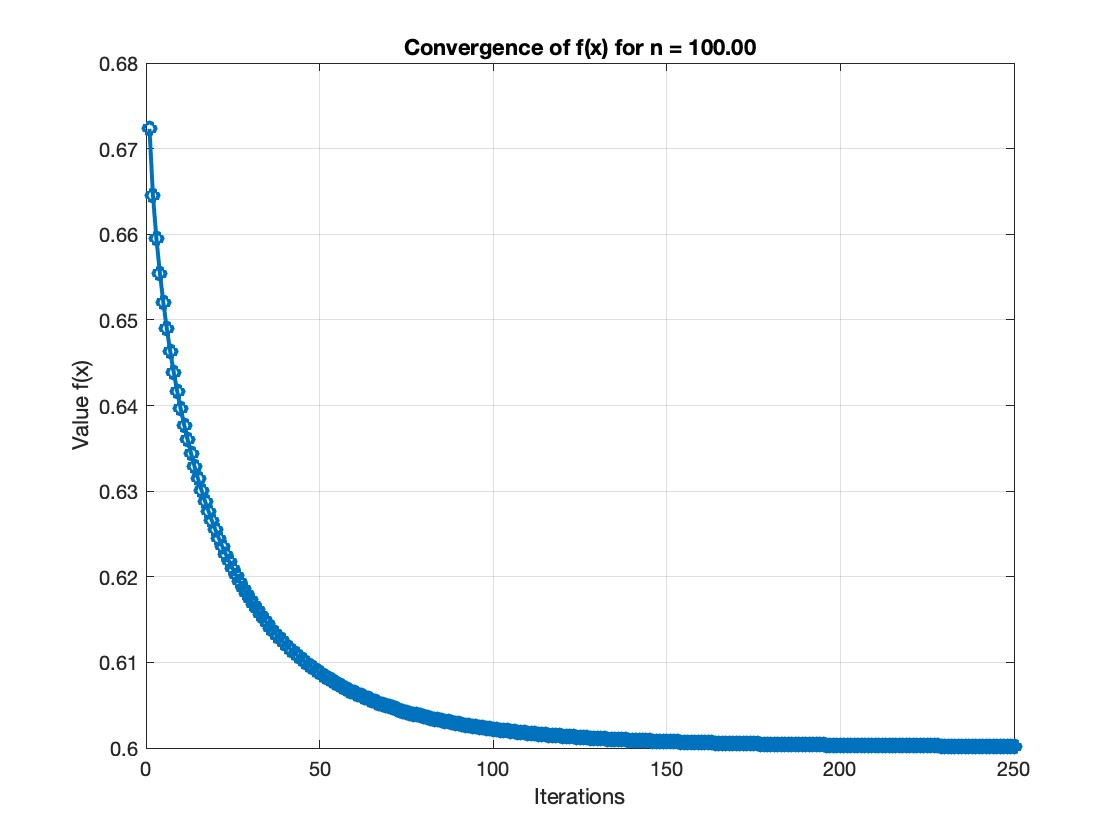
\includegraphics[width=\textwidth]{23f25.jpg}
%    \end{subfigure}
%    \begin{subfigure}[b]{0.45\textwidth}
%        \centering
%        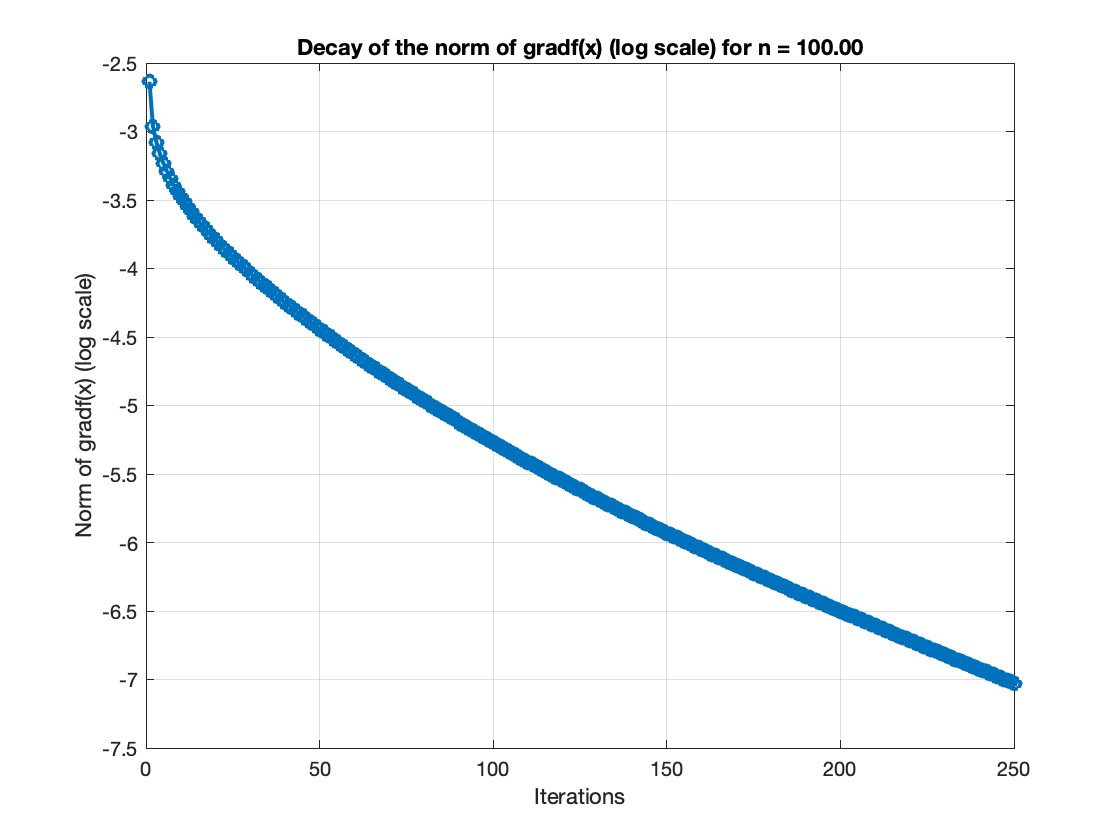
\includegraphics[width=\textwidth]{23g25.jpg}
%    \end{subfigure}
%    \caption{Experiment $25$ for $(2, 100)$}

%    \newpage

%    \begin{subfigure}[b]{0.45\textwidth}
%        \centering
%        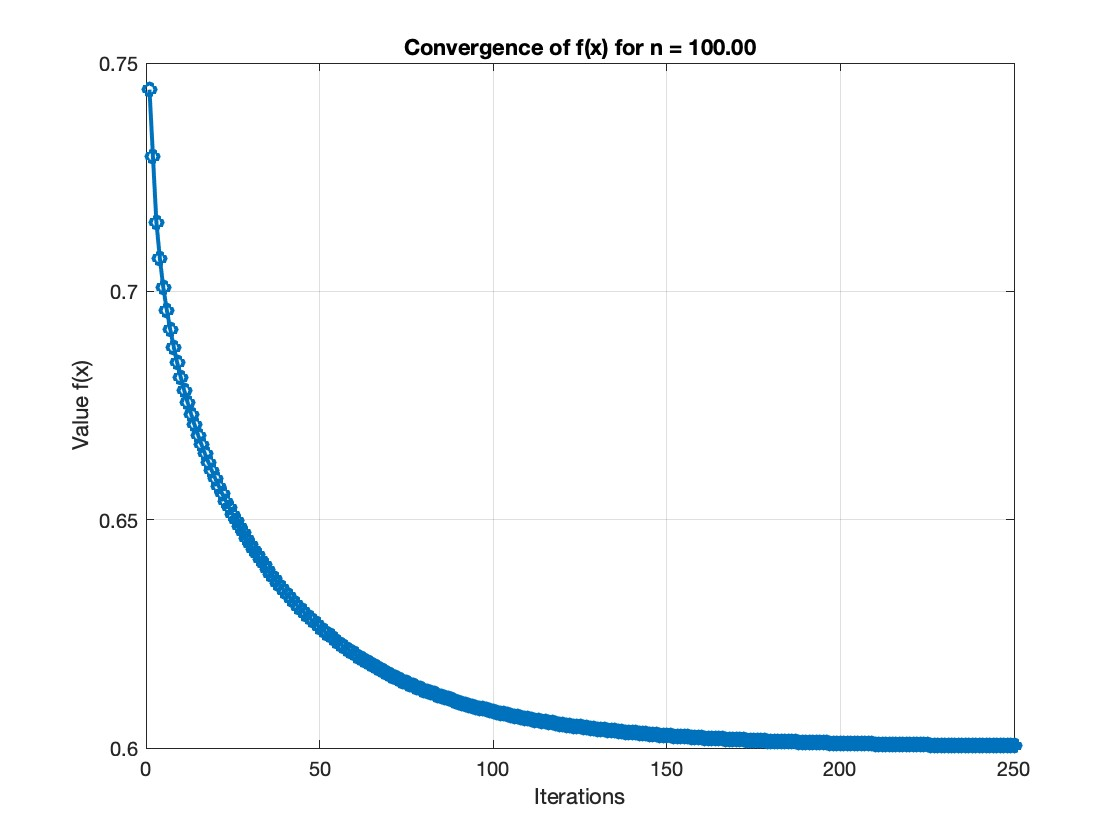
\includegraphics[width=\textwidth]{23f26.jpg}
%    \end{subfigure}
%    \begin{subfigure}[b]{0.45\textwidth}
%        \centering
%        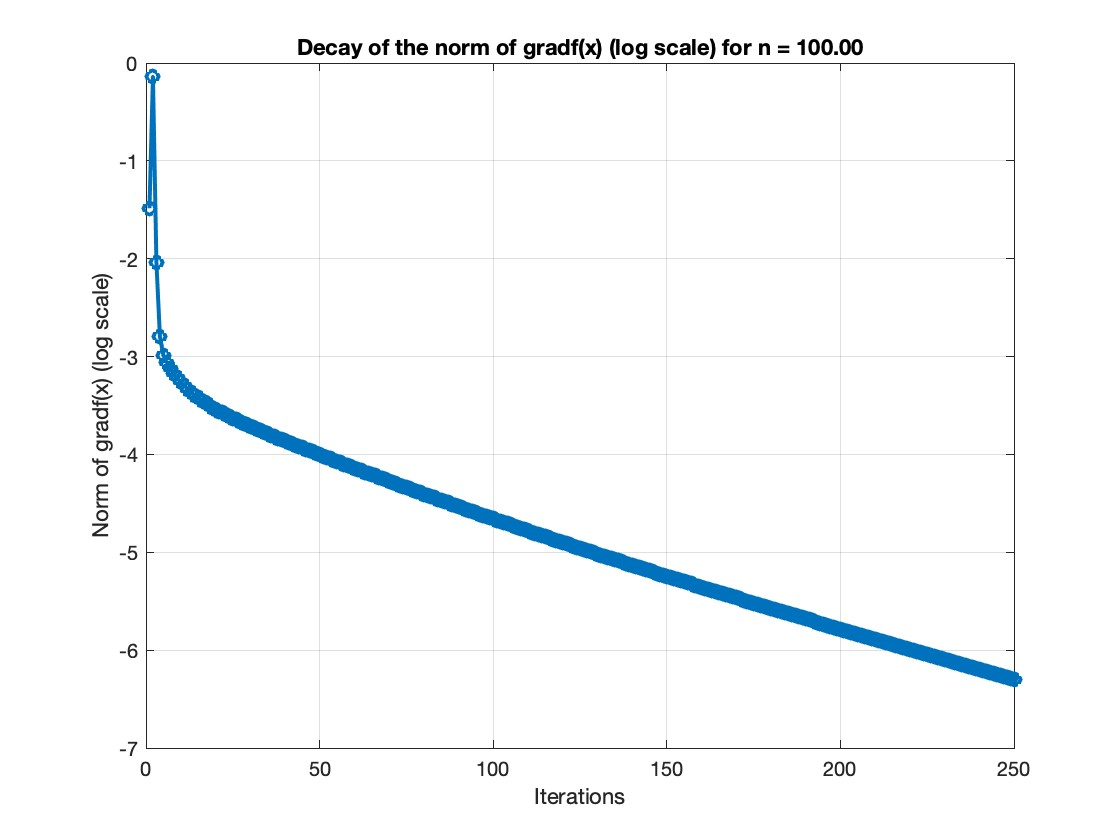
\includegraphics[width=\textwidth]{23g26.jpg}
%    \end{subfigure}
%    \caption{Experiment $26$ for $(2, 100)$}

%    \newpage

%    \begin{subfigure}[b]{0.45\textwidth}
%        \centering
%        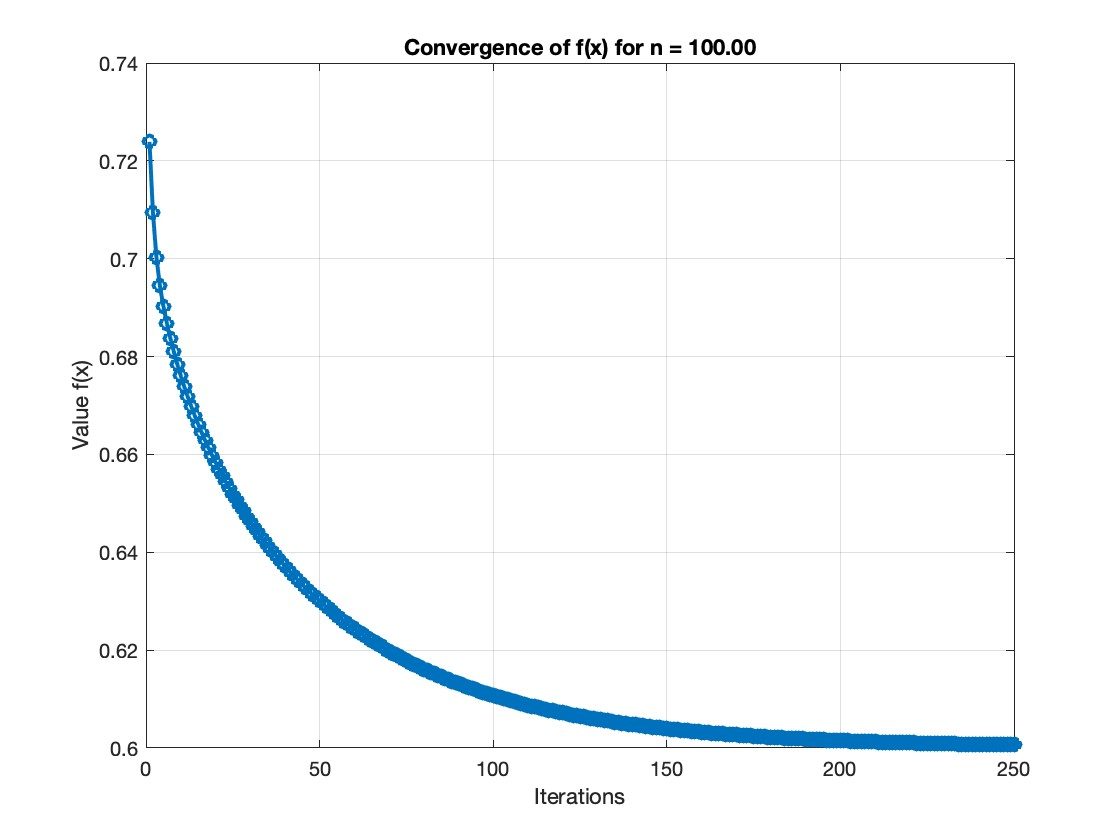
\includegraphics[width=\textwidth]{23f27.jpg}
%    \end{subfigure}
%    \begin{subfigure}[b]{0.45\textwidth}
%        \centering
%        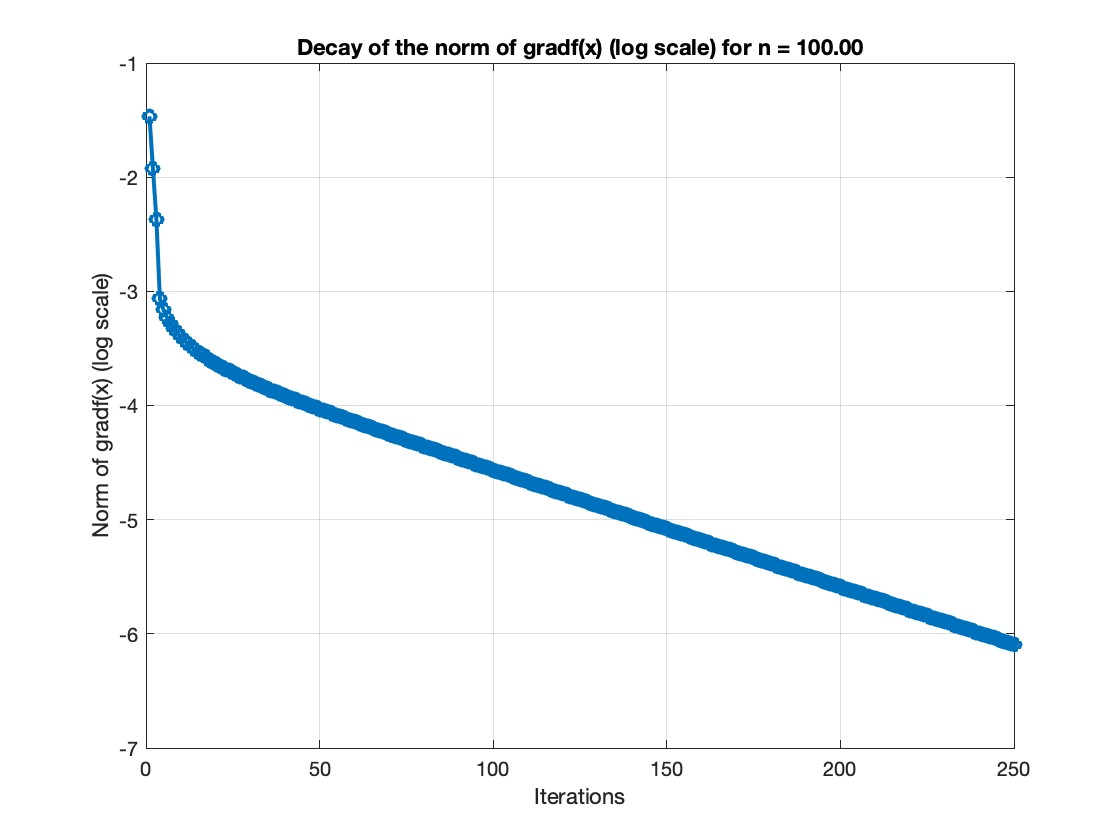
\includegraphics[width=\textwidth]{23g27.jpg}
%    \end{subfigure}
%    \caption{Experiment $27$ for $(2, 100)$}

%    \newpage

%    \begin{subfigure}[b]{0.45\textwidth}
%        \centering
%        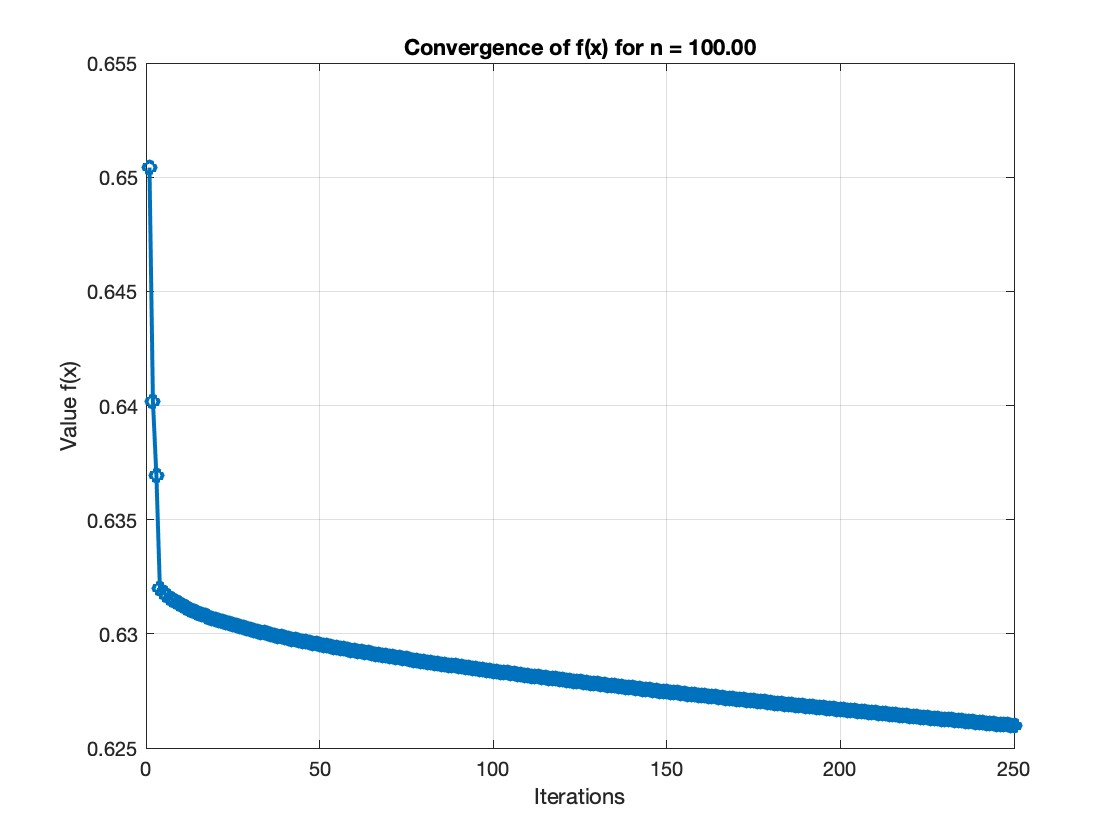
\includegraphics[width=\textwidth]{23f28.jpg}
%    \end{subfigure}
%    \begin{subfigure}[b]{0.45\textwidth}
%        \centering
%        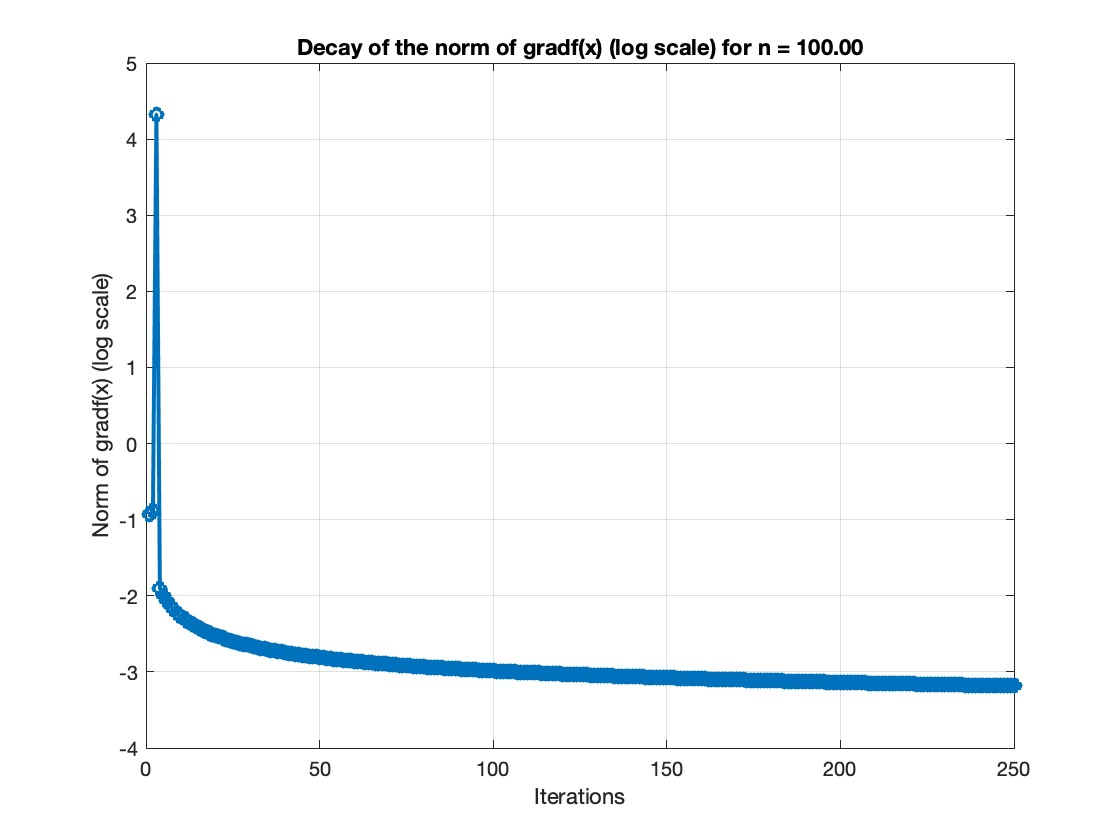
\includegraphics[width=\textwidth]{23g28.jpg}
%    \end{subfigure}
%    \caption{Experiment $28$ for $(2, 100)$}
%\end{figure}
%\begin{figure}
%    \centering
%    \begin{subfigure}[b]{0.45\textwidth}
%        \centering
%        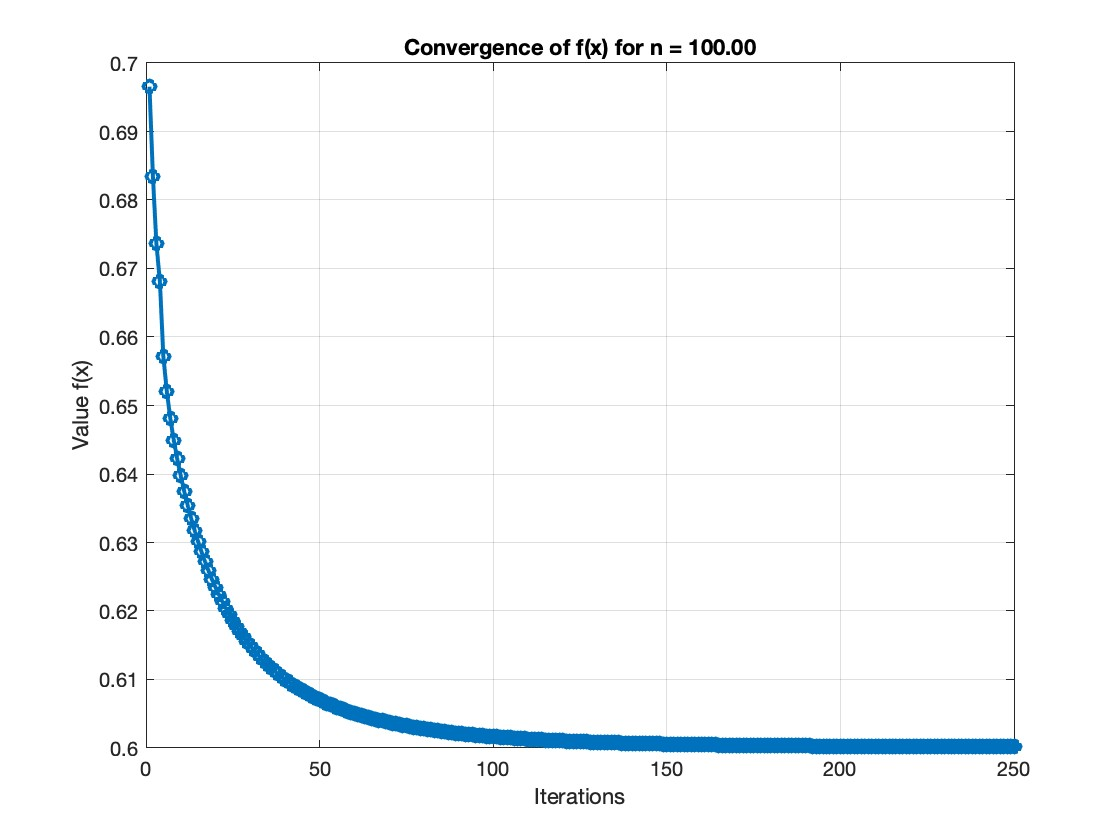
\includegraphics[width=\textwidth]{23f29.jpg}
%    \end{subfigure}
%    \begin{subfigure}[b]{0.45\textwidth}
%        \centering
%        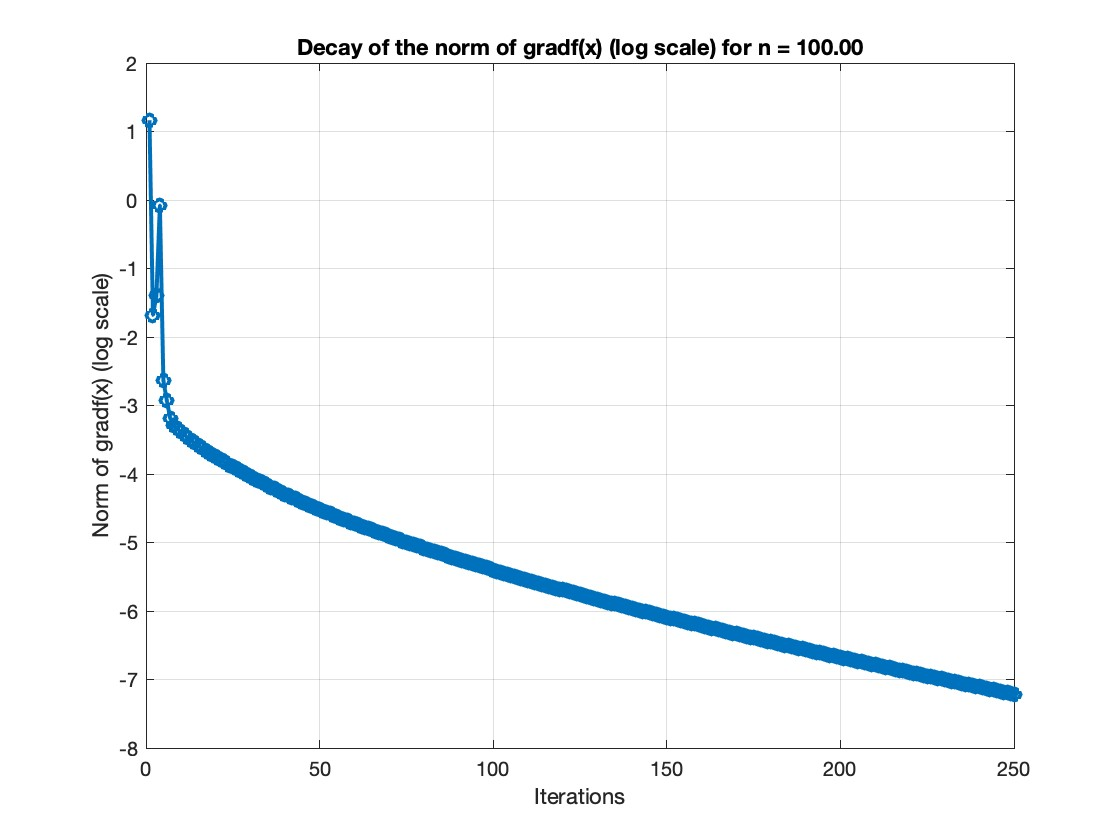
\includegraphics[width=\textwidth]{23g29.jpg}
%    \end{subfigure}
%    \caption{Experiment $29$ for $(2, 100)$}

%    \newpage

%    \begin{subfigure}[b]{0.45\textwidth}
%        \centering
%        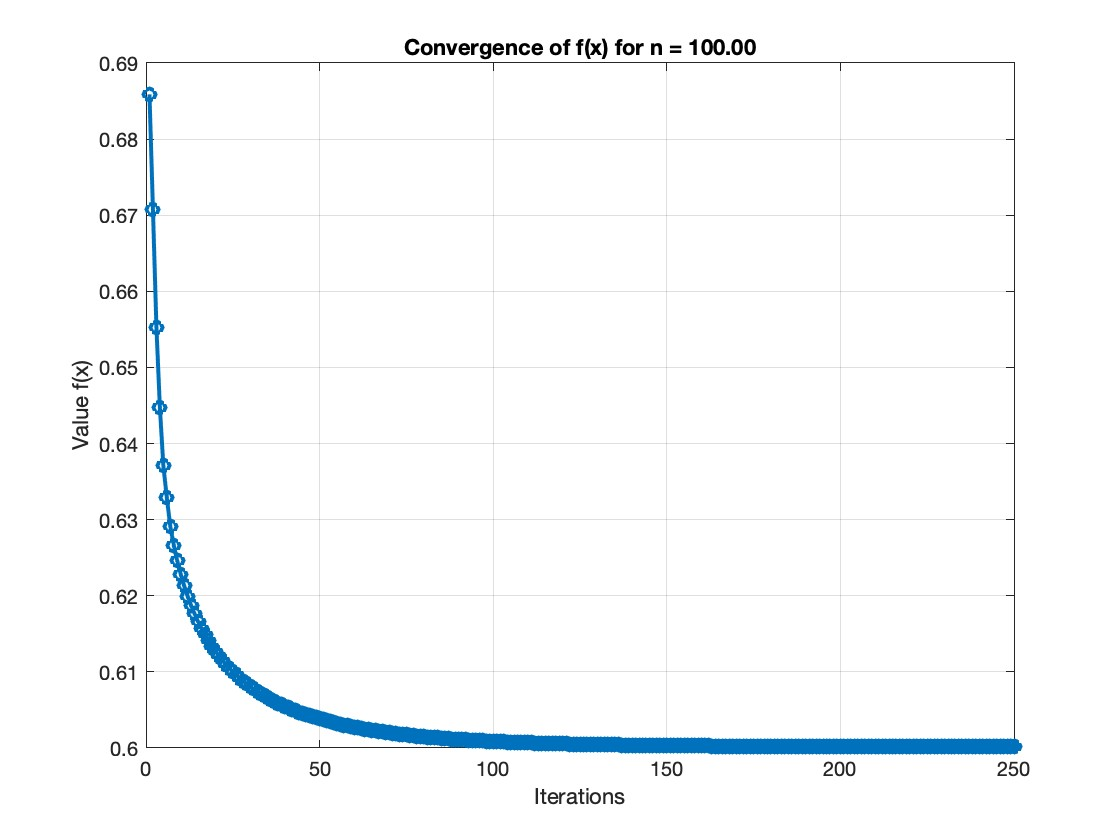
\includegraphics[width=\textwidth]{23f30.jpg}
%    \end{subfigure}
%    \begin{subfigure}[b]{0.45\textwidth}
%        \centering
%        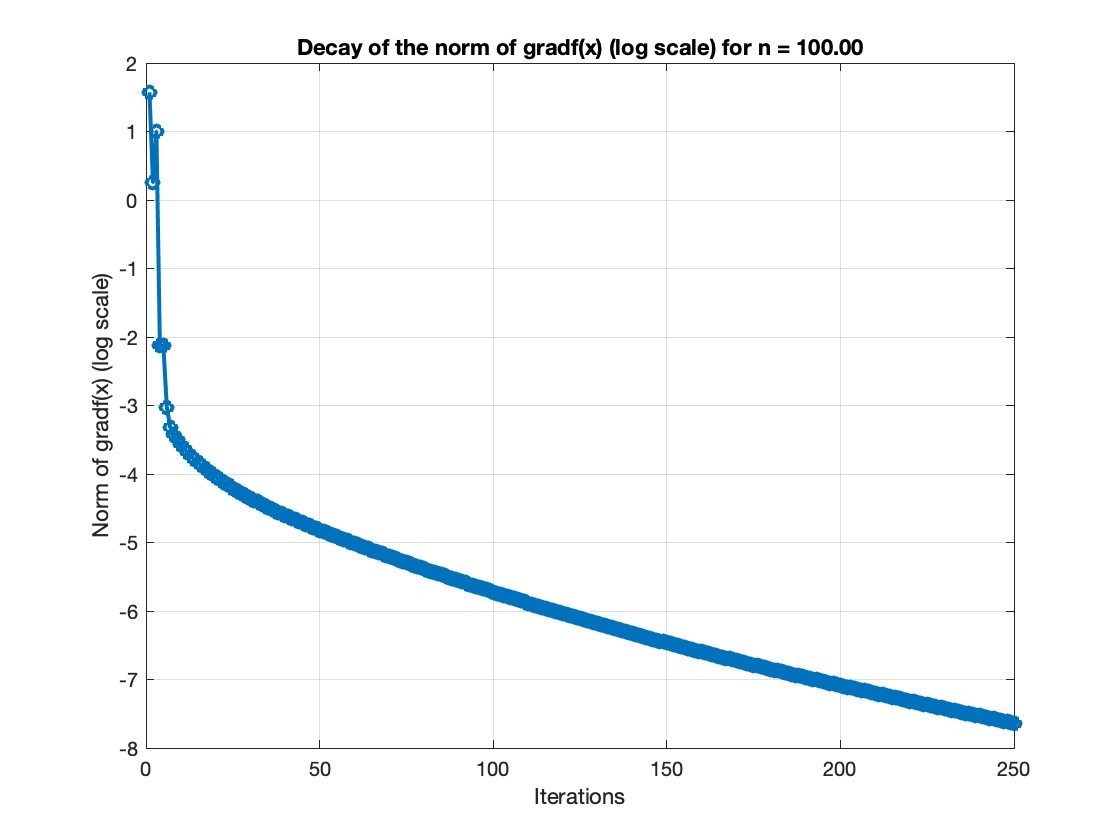
\includegraphics[width=\textwidth]{23g30.jpg}
%    \end{subfigure}
%    \caption{Experiment $30$ for $(2, 100)$}
%    \label{fig:2330}
%\end{figure}

We now perform the same work with the pair $(3, 128)$. Figure \ref{fig:32} gives the graphs of the function values and gradient norms (in log scale) for the best experiment, which was the second. As previously, we notice that $f$ decays exponentially fast. Moreover, despite not converging in $250$ iterations, it still decreases considerably and seems to approach a value between $0.26$ and $0.27$. As for the gradient, it decays first very fast and then linearly (on the log scale).\\

\begin{figure}[H]
    \centering
    %\begin{subfigure}[b]{0.45\textwidth}
    %    \centering
    %    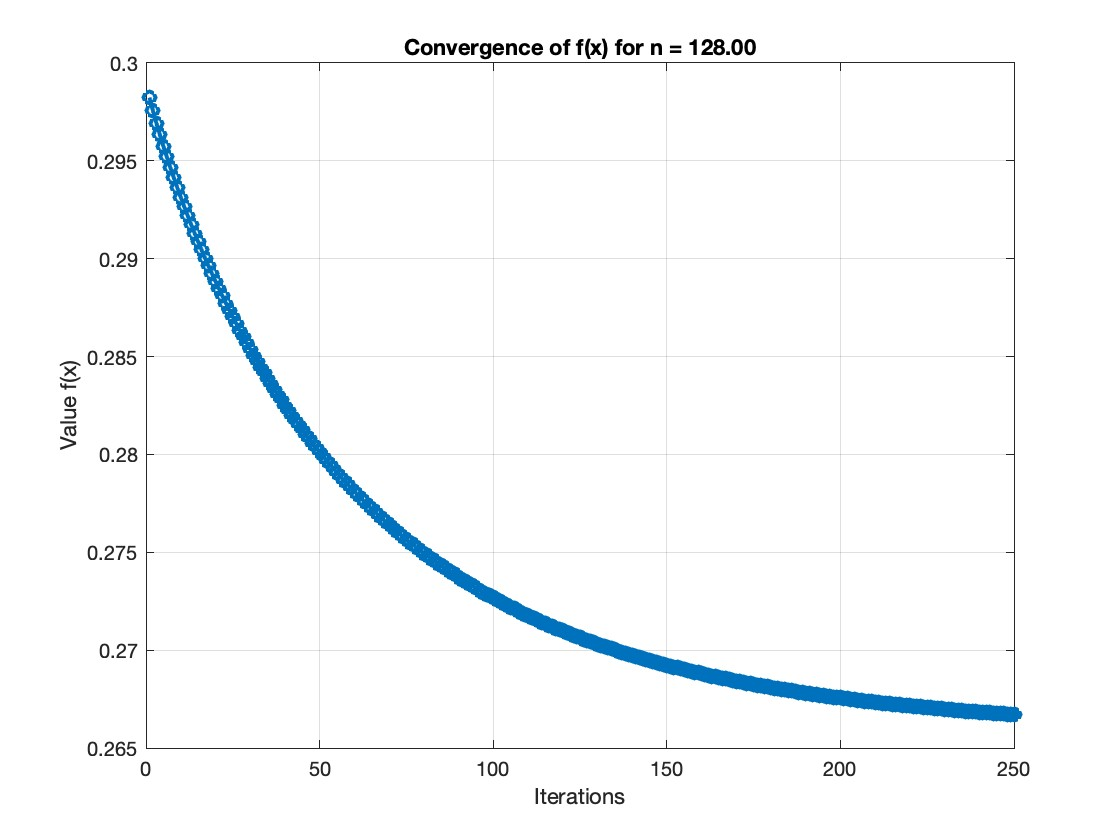
\includegraphics[width=\textwidth]{3f1.jpg}
    %\end{subfigure}
    %\begin{subfigure}[b]{0.45\textwidth}
    %    \centering
    %    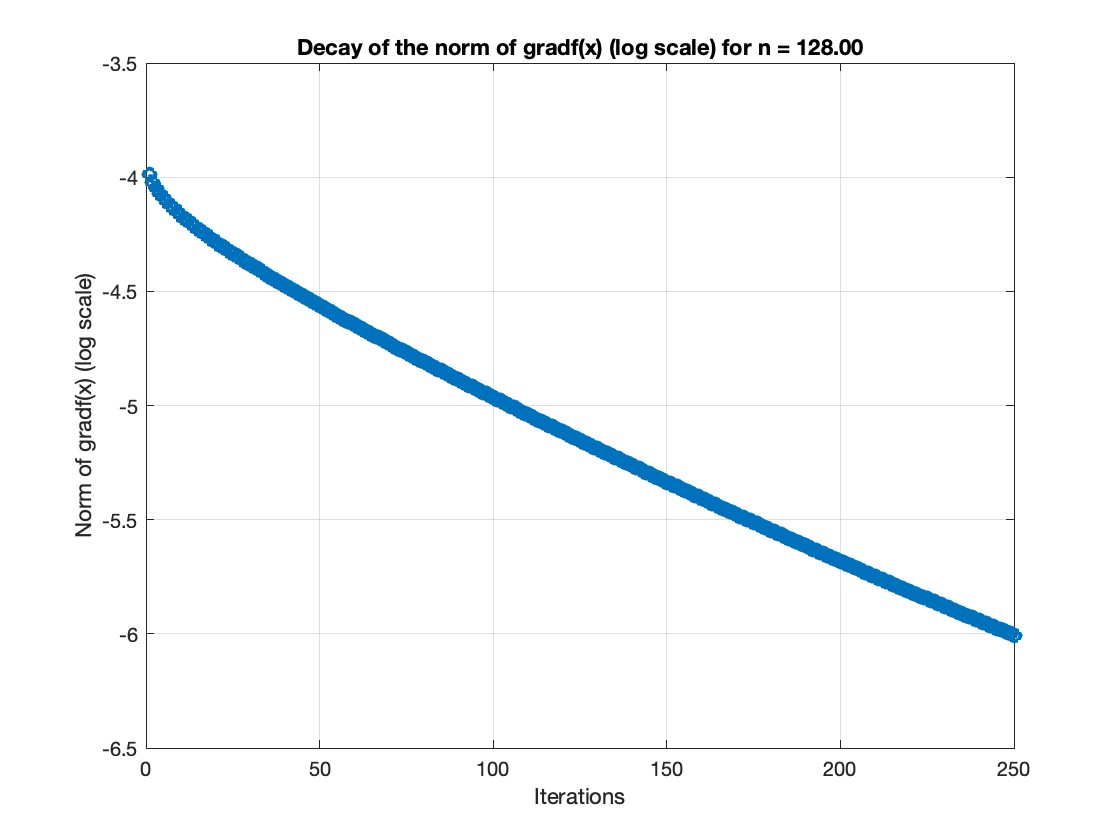
\includegraphics[width=\textwidth]{3g1.jpg}
    %\end{subfigure}
    %\caption{Experiment $1$ for $(3, 128)$}
    %\label{fig:31}
    
    %\newpage

    \begin{subfigure}[b]{0.49\textwidth}
        \centering
        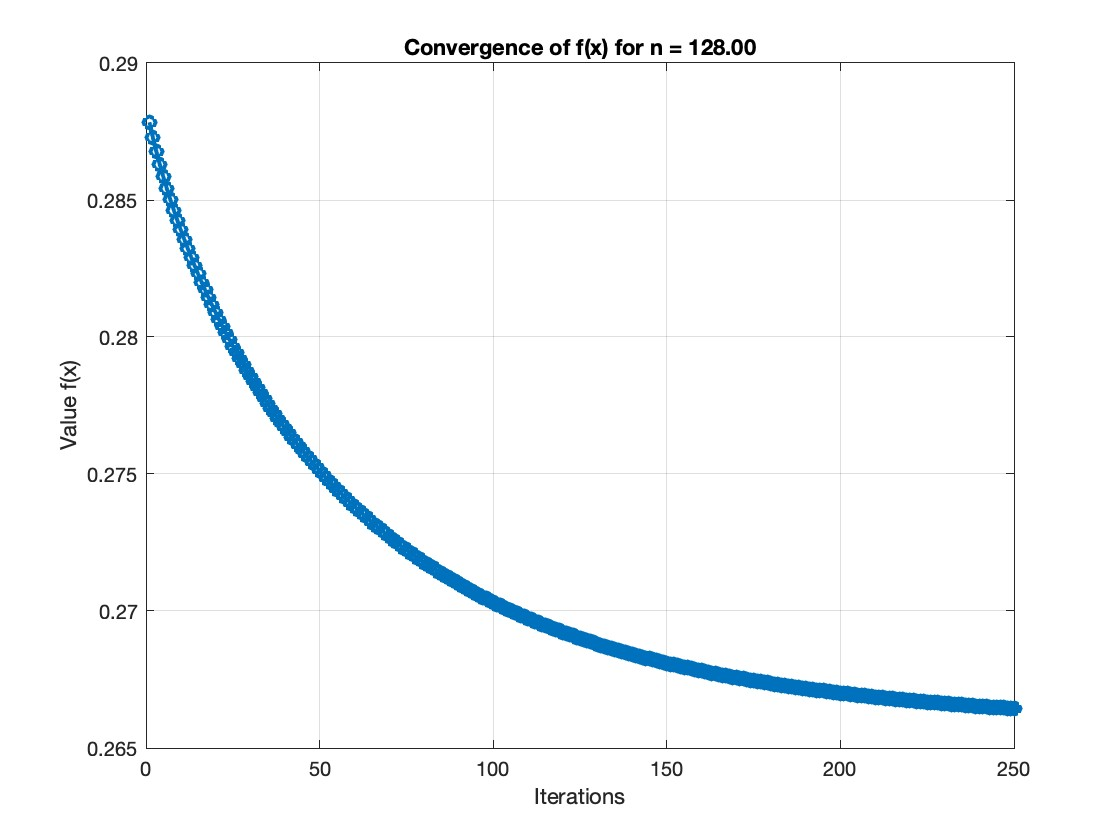
\includegraphics[width=\textwidth]{3f2.jpg}
    \end{subfigure}
    \begin{subfigure}[b]{0.49\textwidth}
        \centering
        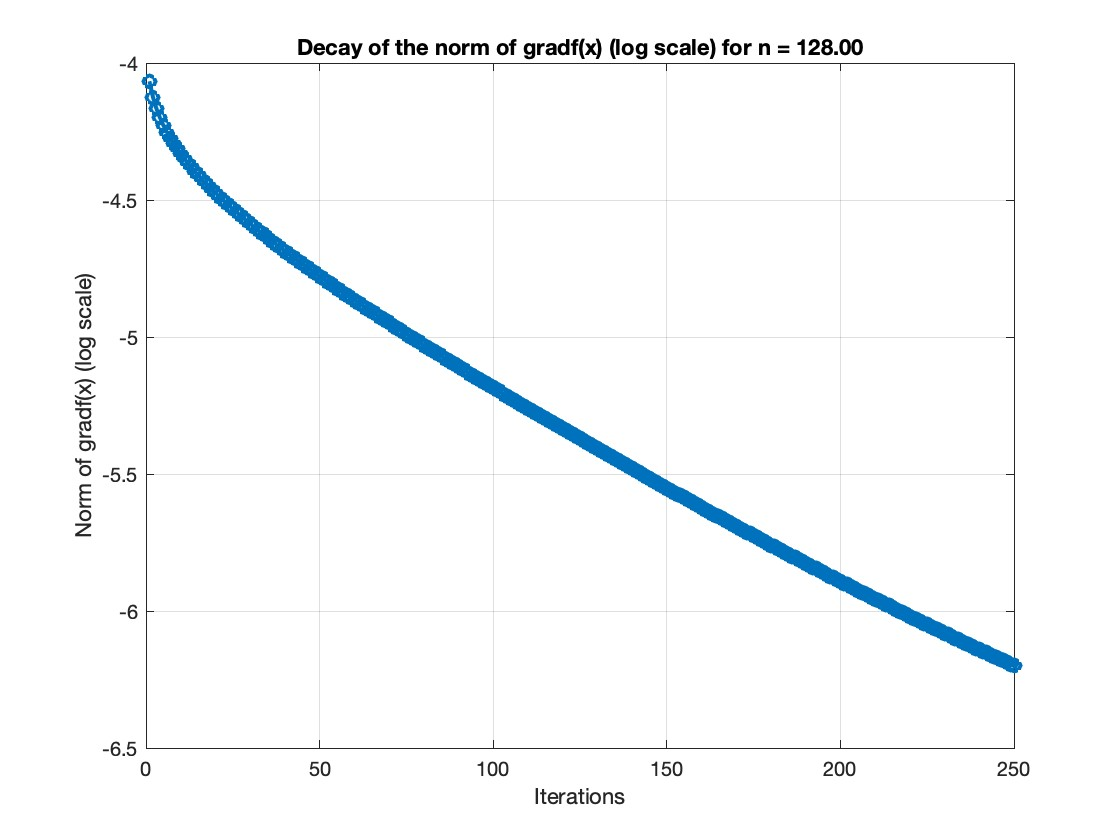
\includegraphics[width=\textwidth]{3g2.jpg}
    \end{subfigure}
    \caption{Experiment $2$ for $(3, 128)$, corresponding to the best configuration obtained}
    \label{fig:32}
    
    %\newpage

    %\begin{subfigure}[b]{0.45\textwidth}
    %    \centering
    %    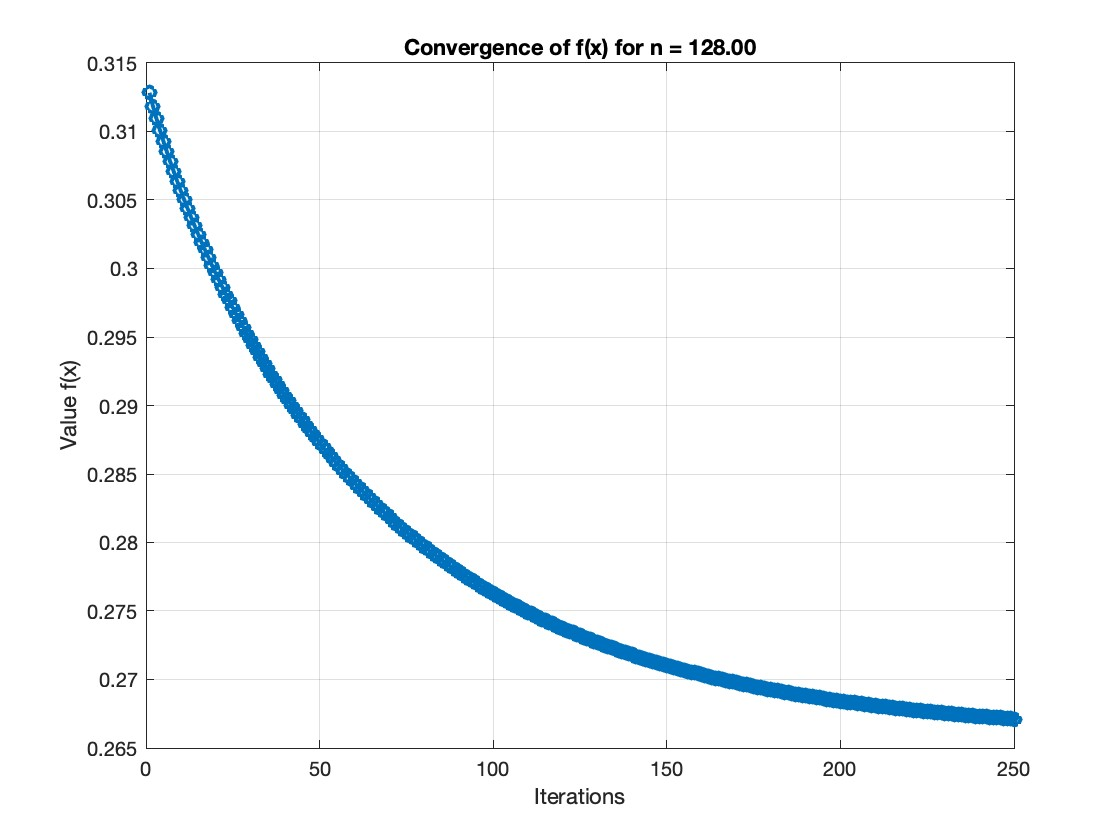
\includegraphics[width=\textwidth]{3f3.jpg}
    %\end{subfigure}
    %\begin{subfigure}[b]{0.45\textwidth}
    %    \centering
    %    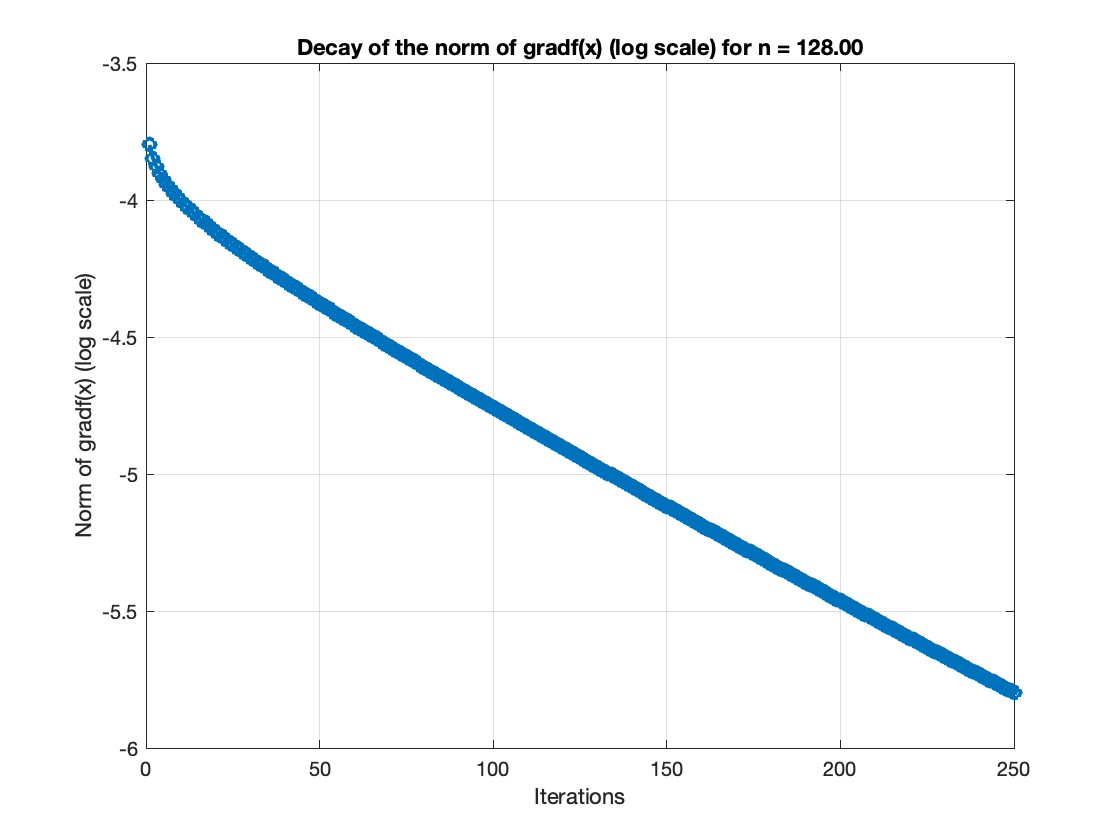
\includegraphics[width=\textwidth]{3g3.jpg}
    %\end{subfigure}
    %\caption{Experiment $3$ for $(3, 128)$}

    %\newpage

    %\begin{subfigure}[b]{0.45\textwidth}
    %    \centering
    %    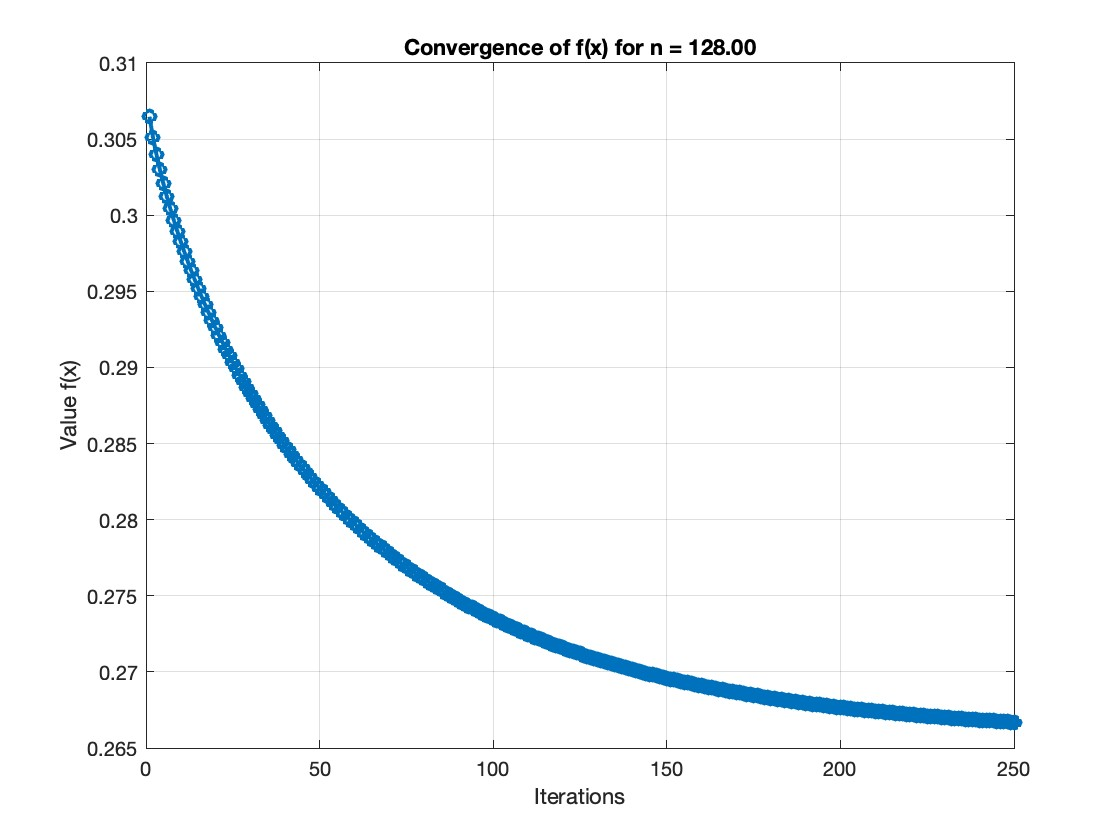
\includegraphics[width=\textwidth]{3f4.jpg}
    %\end{subfigure}
    %\begin{subfigure}[b]{0.45\textwidth}
    %    \centering
    %    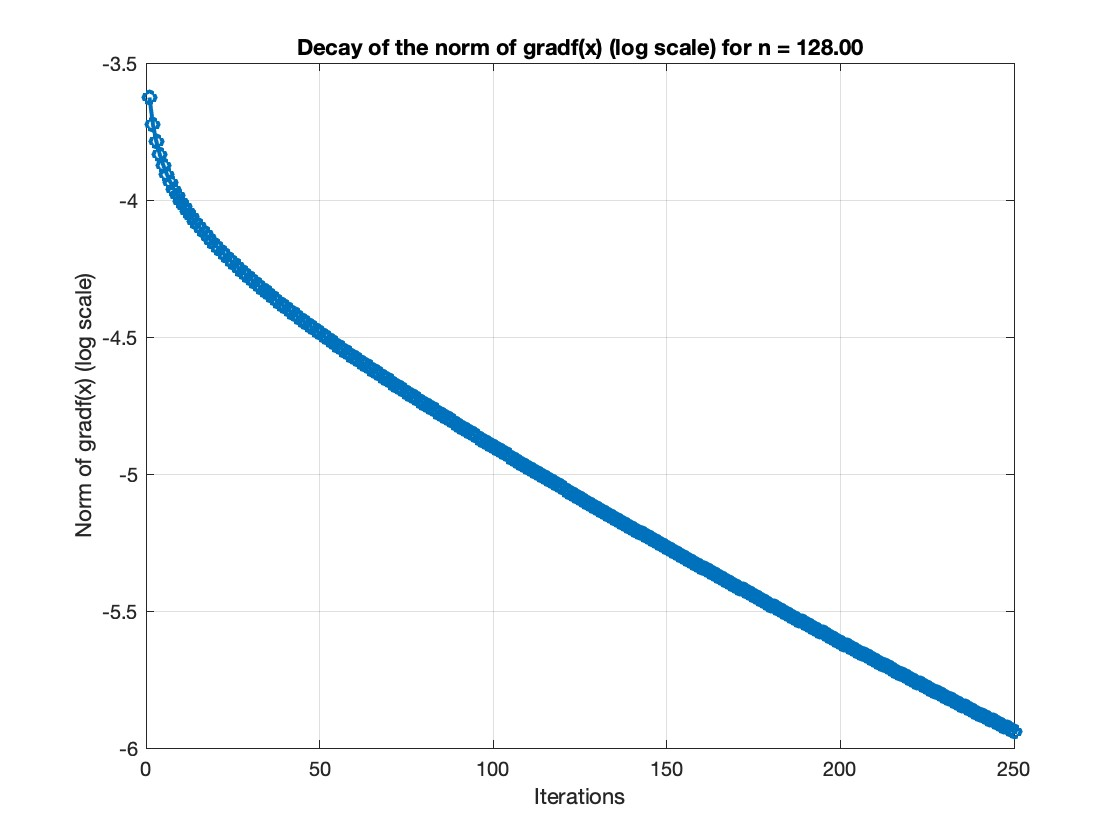
\includegraphics[width=\textwidth]{3g4.jpg}
    %\end{subfigure}
    %\caption{Experiment $4$ for $(3, 128)$}
\end{figure}
%\begin{figure}
%    \centering
%    \begin{subfigure}[b]{0.45\textwidth}
%        \centering
%        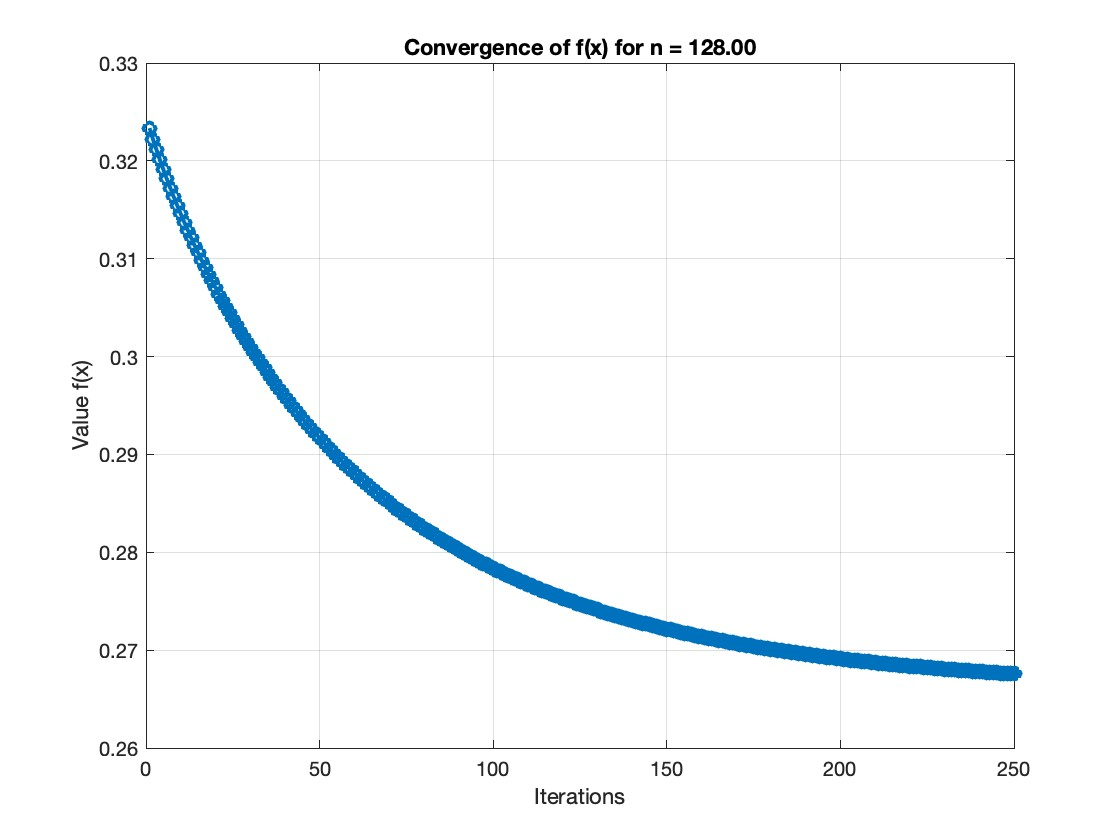
\includegraphics[width=\textwidth]{3f5.jpg}
%    \end{subfigure}
%    \begin{subfigure}[b]{0.45\textwidth}
%        \centering
%        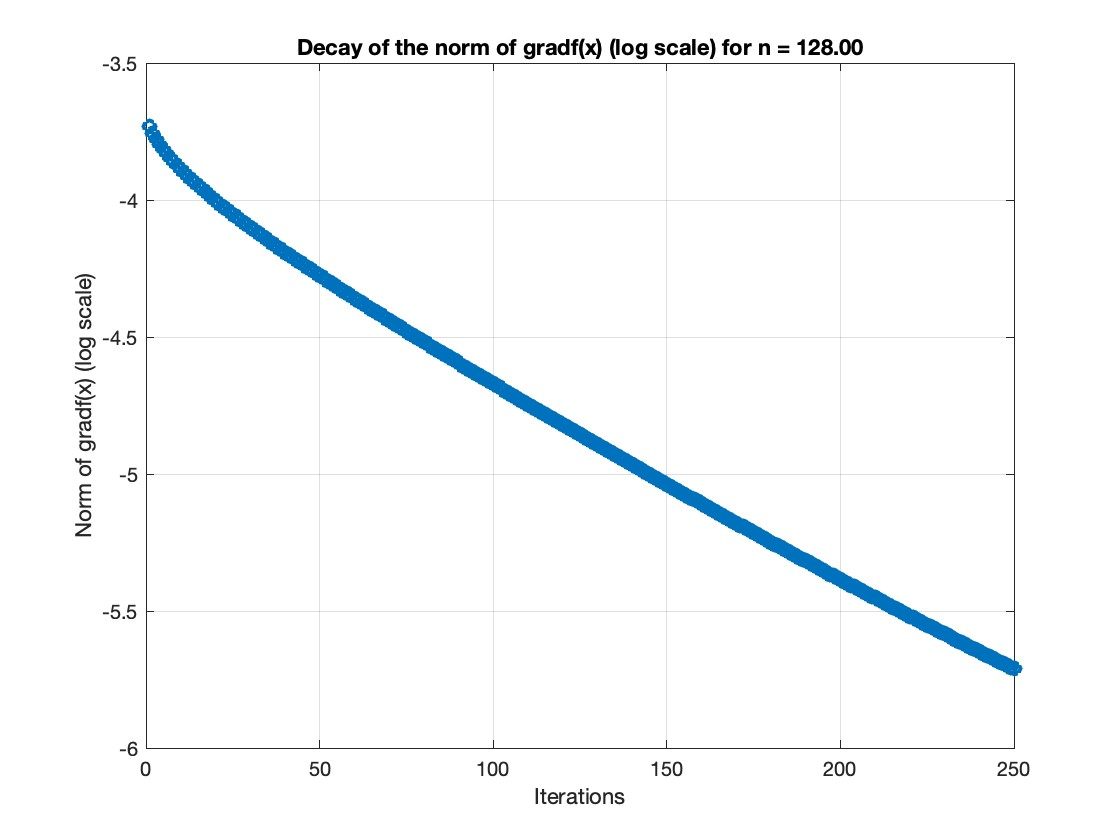
\includegraphics[width=\textwidth]{3g5.jpg}
%    \end{subfigure}
%    \caption{Experiment $5$ for $(3, 128)$}

%    \newpage

%    \begin{subfigure}[b]{0.45\textwidth}
%        \centering
%        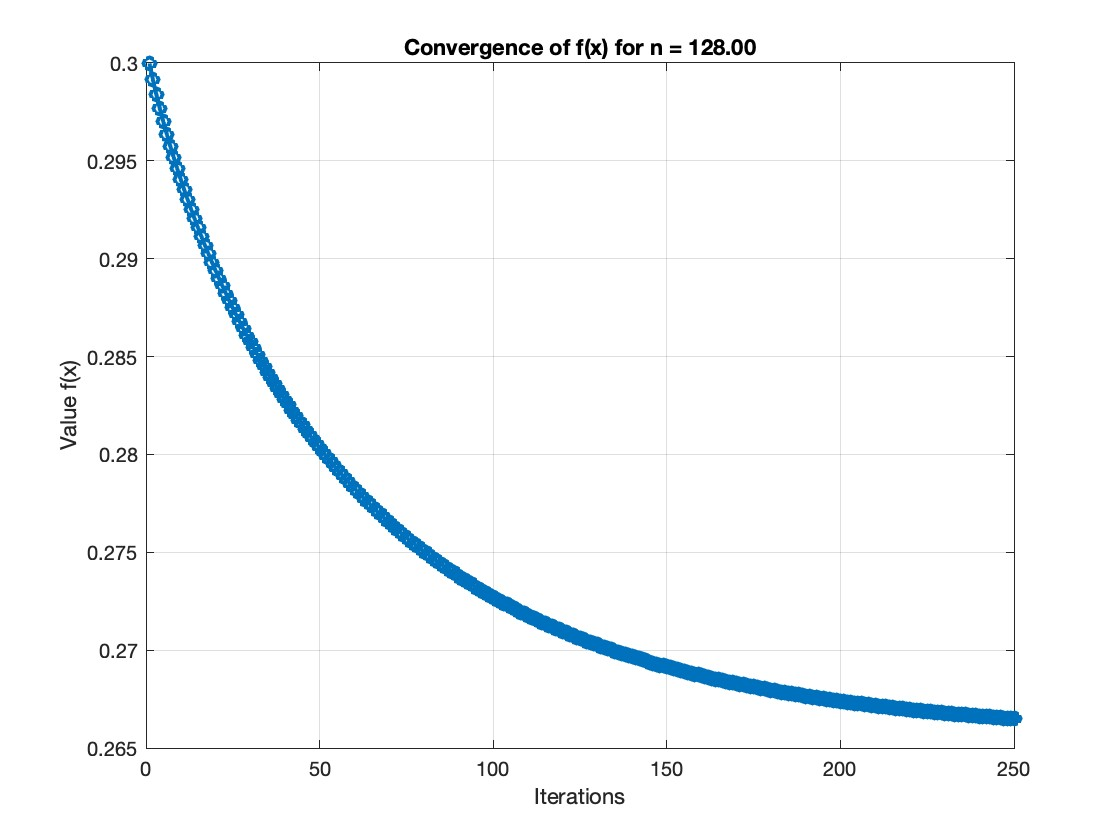
\includegraphics[width=\textwidth]{3f6.jpg}
%    \end{subfigure}
%    \begin{subfigure}[b]{0.45\textwidth}
%        \centering
%        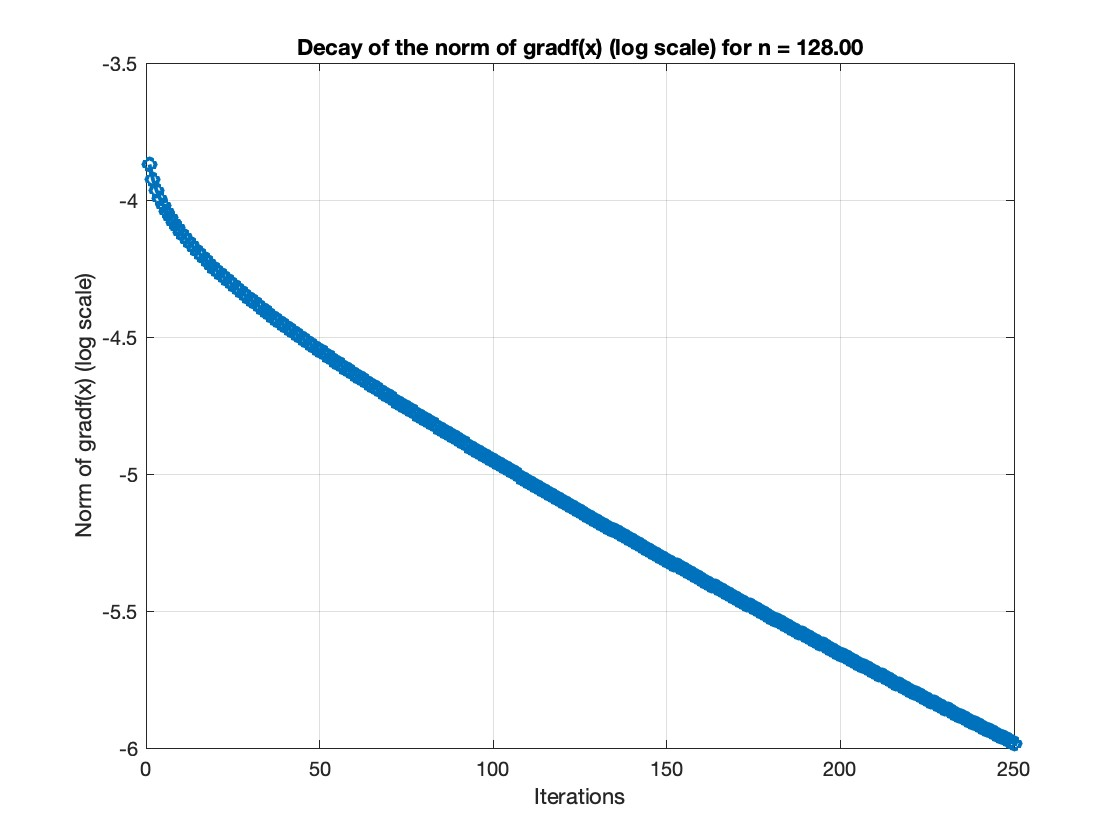
\includegraphics[width=\textwidth]{3g6.jpg}
%    \end{subfigure}
%    \caption{Experiment $6$ for $(3, 128)$}

%    \newpage

%    \begin{subfigure}[b]{0.45\textwidth}
%        \centering
%        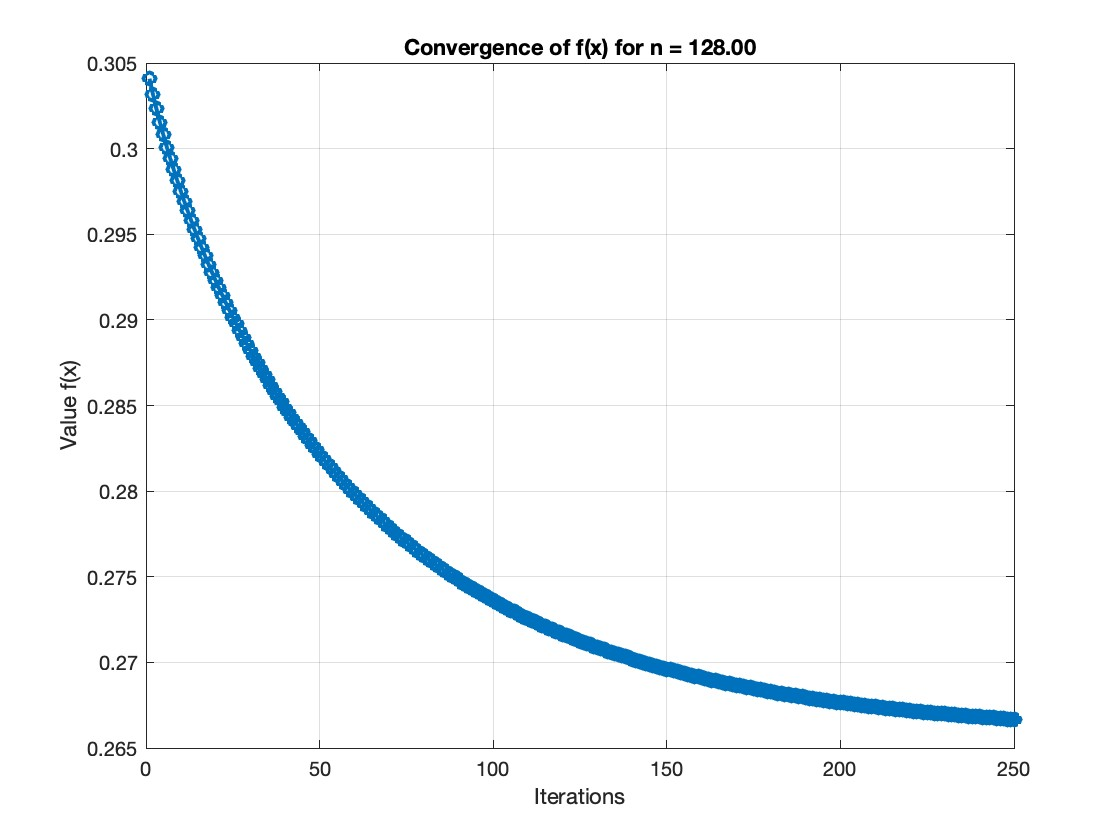
\includegraphics[width=\textwidth]{3f7.jpg}
%    \end{subfigure}
%    \begin{subfigure}[b]{0.45\textwidth}
%        \centering
%        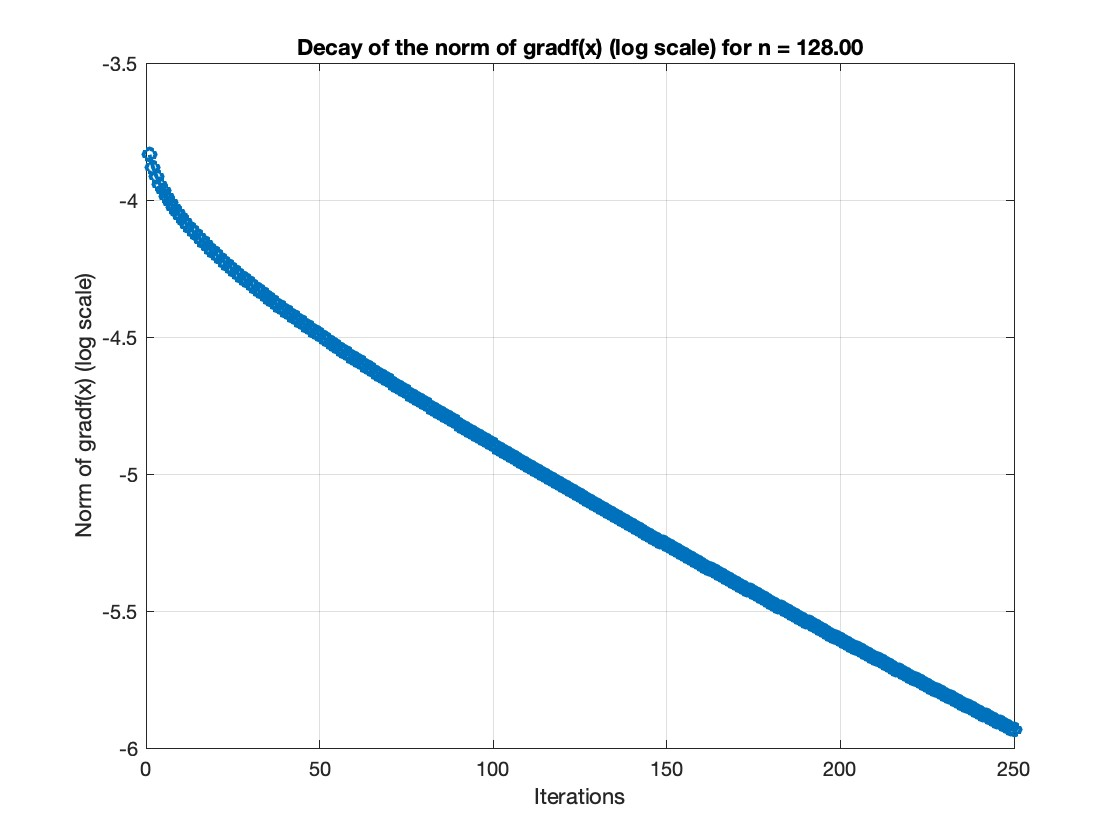
\includegraphics[width=\textwidth]{3g7.jpg}
%    \end{subfigure}
%    \caption{Experiment $7$ for $(3, 128)$}

%    \newpage

%    \begin{subfigure}[b]{0.45\textwidth}
%        \centering
%        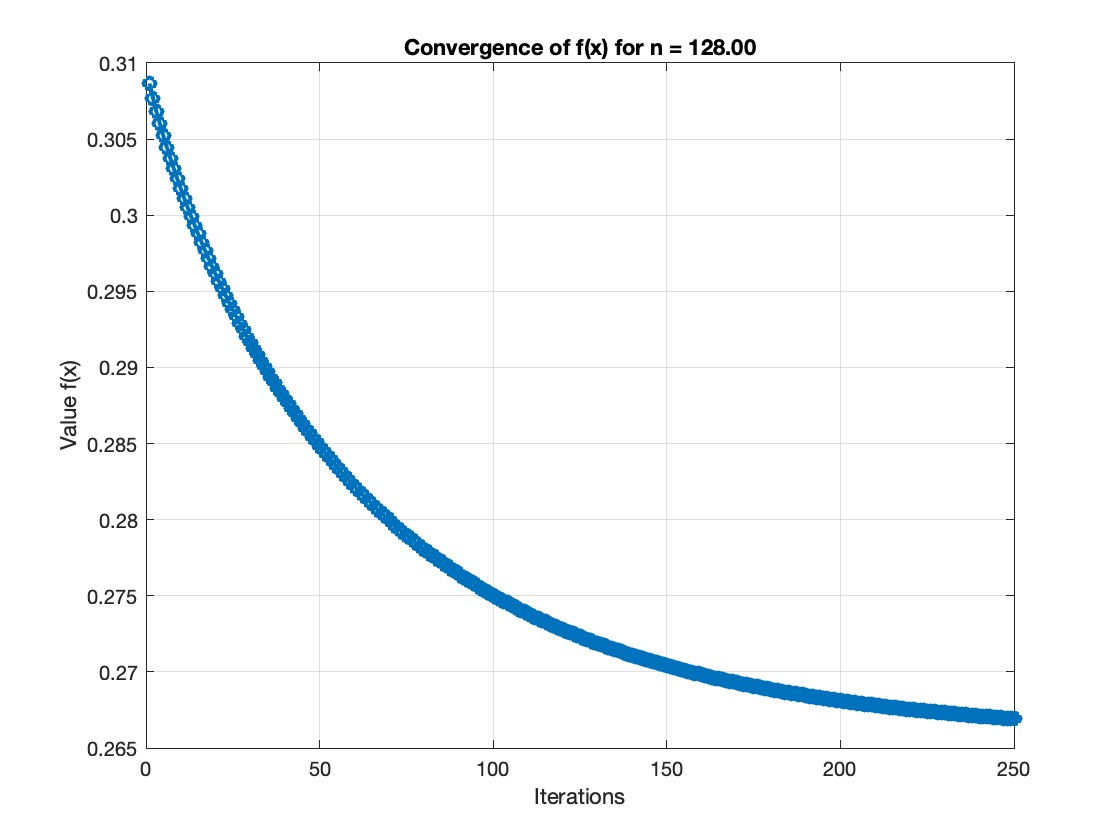
\includegraphics[width=\textwidth]{3f8.jpg}
%    \end{subfigure}
%    \begin{subfigure}[b]{0.45\textwidth}
%        \centering
%        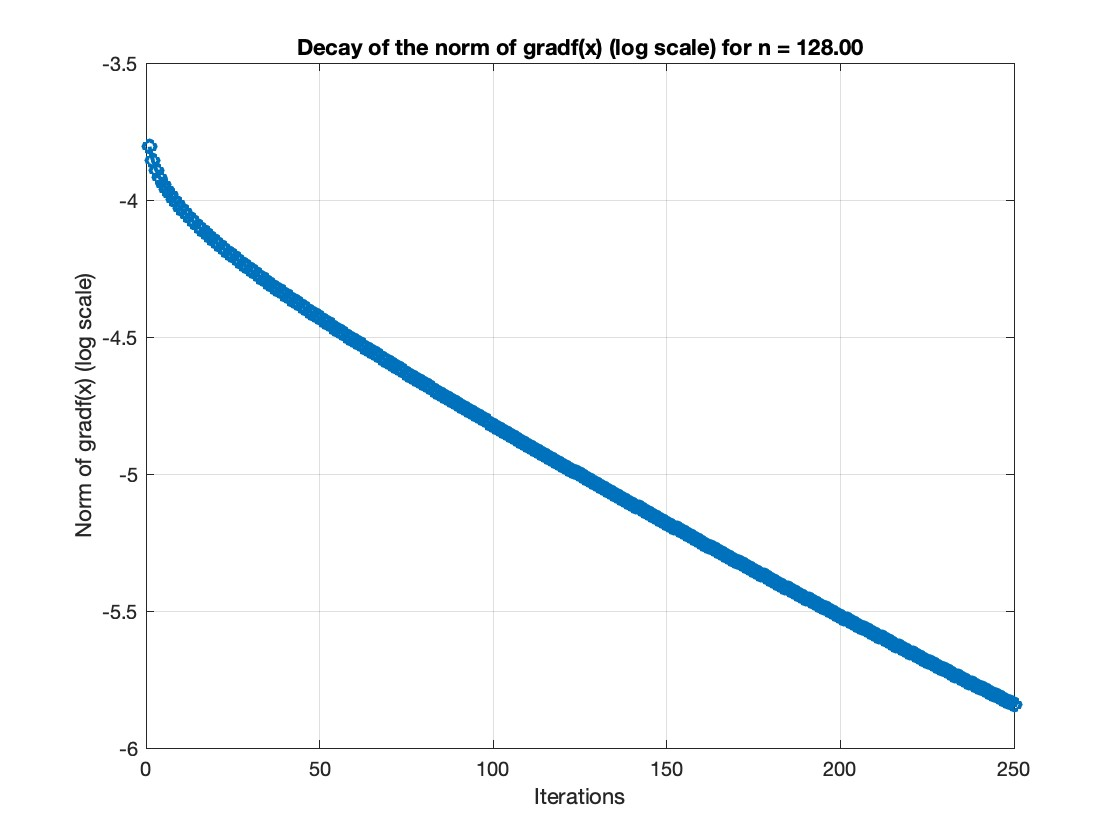
\includegraphics[width=\textwidth]{3g8.jpg}
%    \end{subfigure}
%    \caption{Experiment $8$ for $(3, 128)$}
%\end{figure}
%\begin{figure}
%    \centering
%    \begin{subfigure}[b]{0.45\textwidth}
%        \centering
%        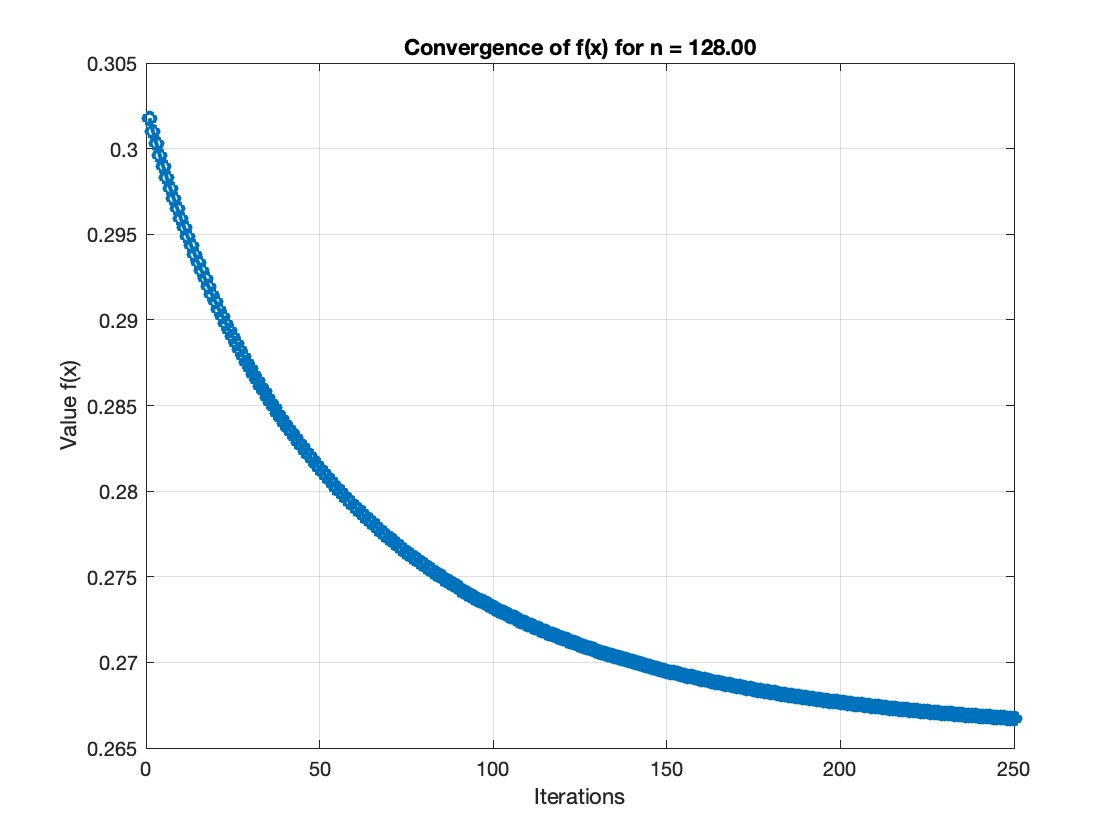
\includegraphics[width=\textwidth]{3f9.jpg}
%    \end{subfigure}
%    \begin{subfigure}[b]{0.45\textwidth}
%        \centering
%        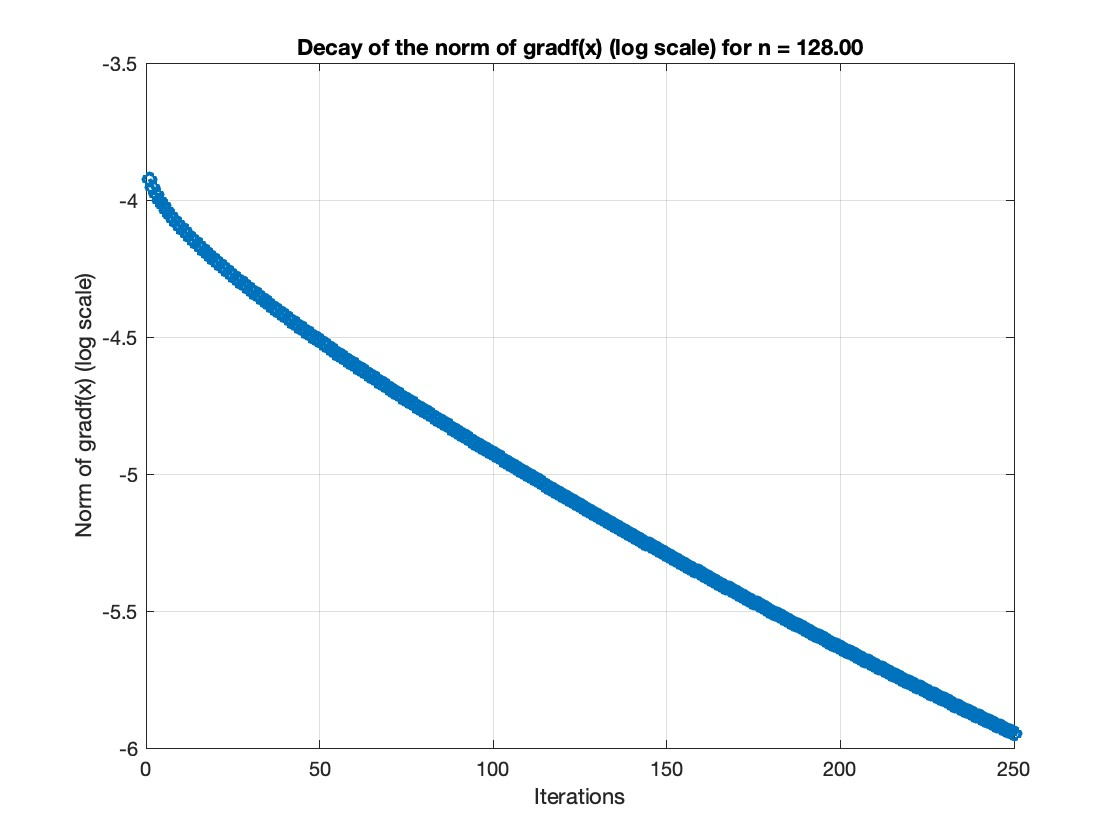
\includegraphics[width=\textwidth]{3g9.jpg}
%    \end{subfigure}
%    \caption{Experiment $9$ for $(3, 128)$}

%    \newpage

%    \begin{subfigure}[b]{0.45\textwidth}
%        \centering
%        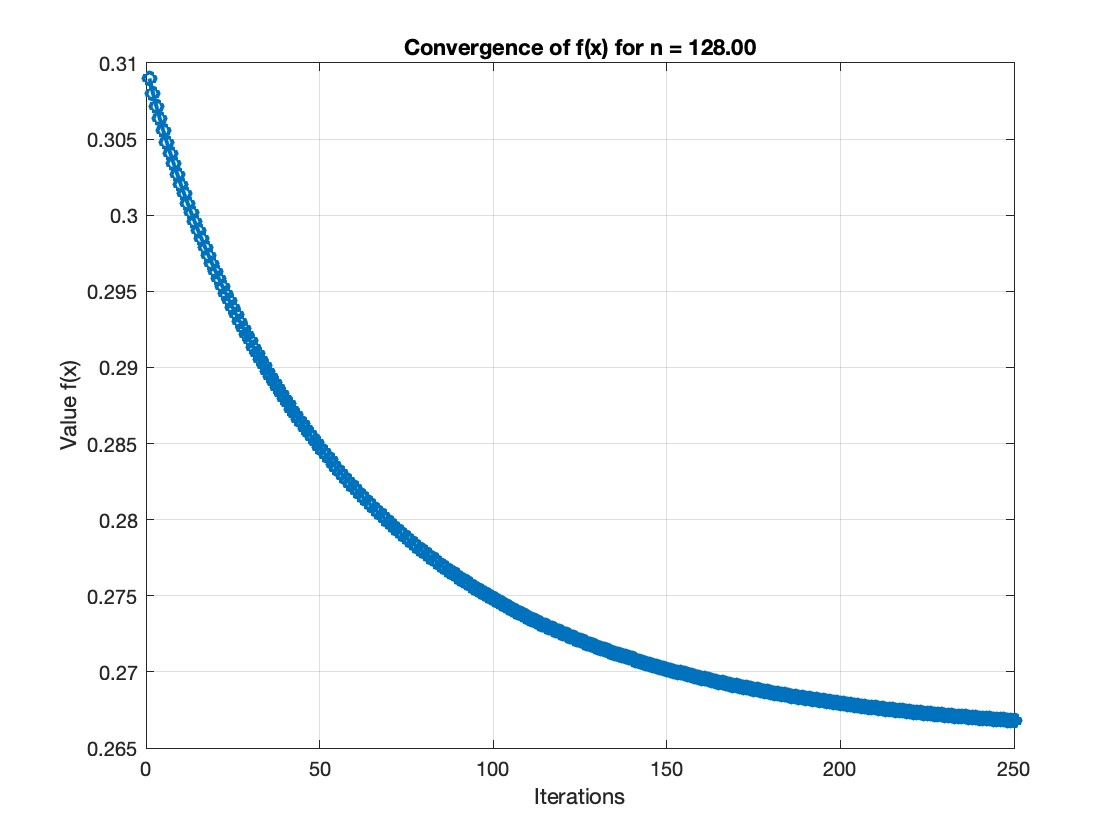
\includegraphics[width=\textwidth]{3f10.jpg}
%    \end{subfigure}
%    \begin{subfigure}[b]{0.45\textwidth}
%        \centering
%        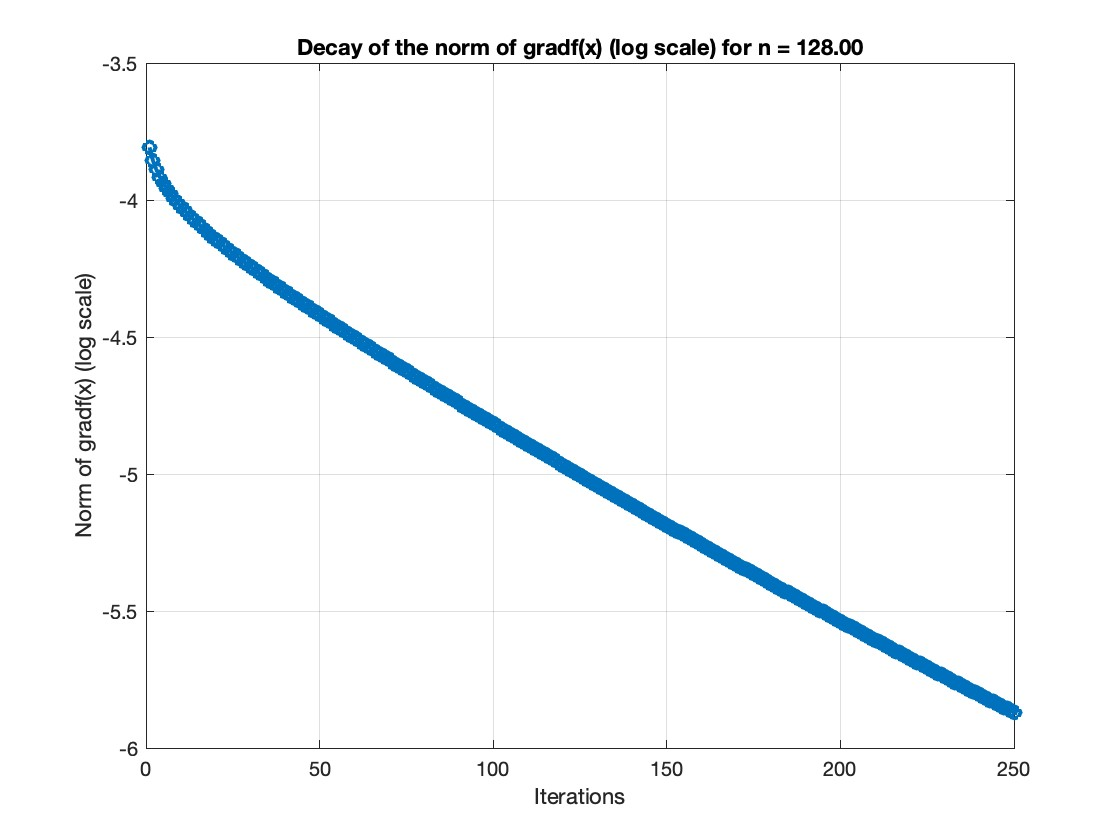
\includegraphics[width=\textwidth]{3g10.jpg}
%    \end{subfigure}
%    \caption{Experiment $10$ for $(3, 128)$}

%    \newpage

%    \begin{subfigure}[b]{0.45\textwidth}
%        \centering
%        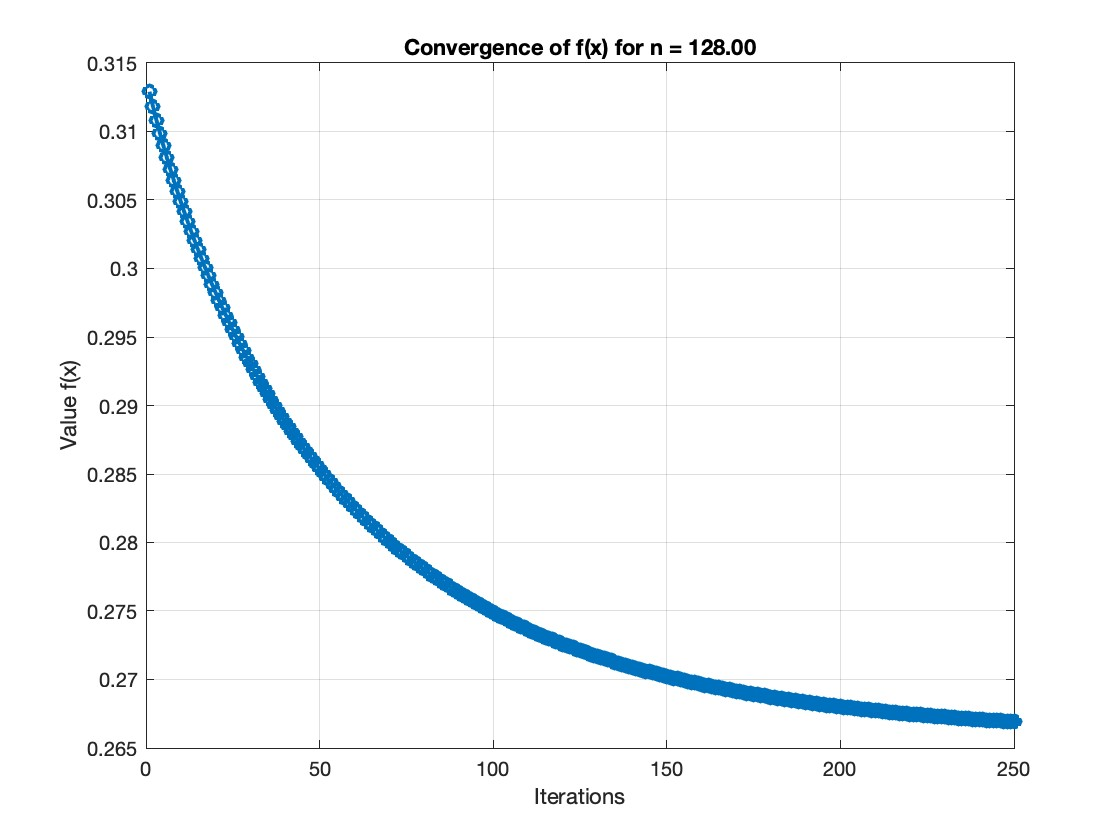
\includegraphics[width=\textwidth]{3f11.jpg}
%    \end{subfigure}
%    \begin{subfigure}[b]{0.45\textwidth}
%        \centering
%        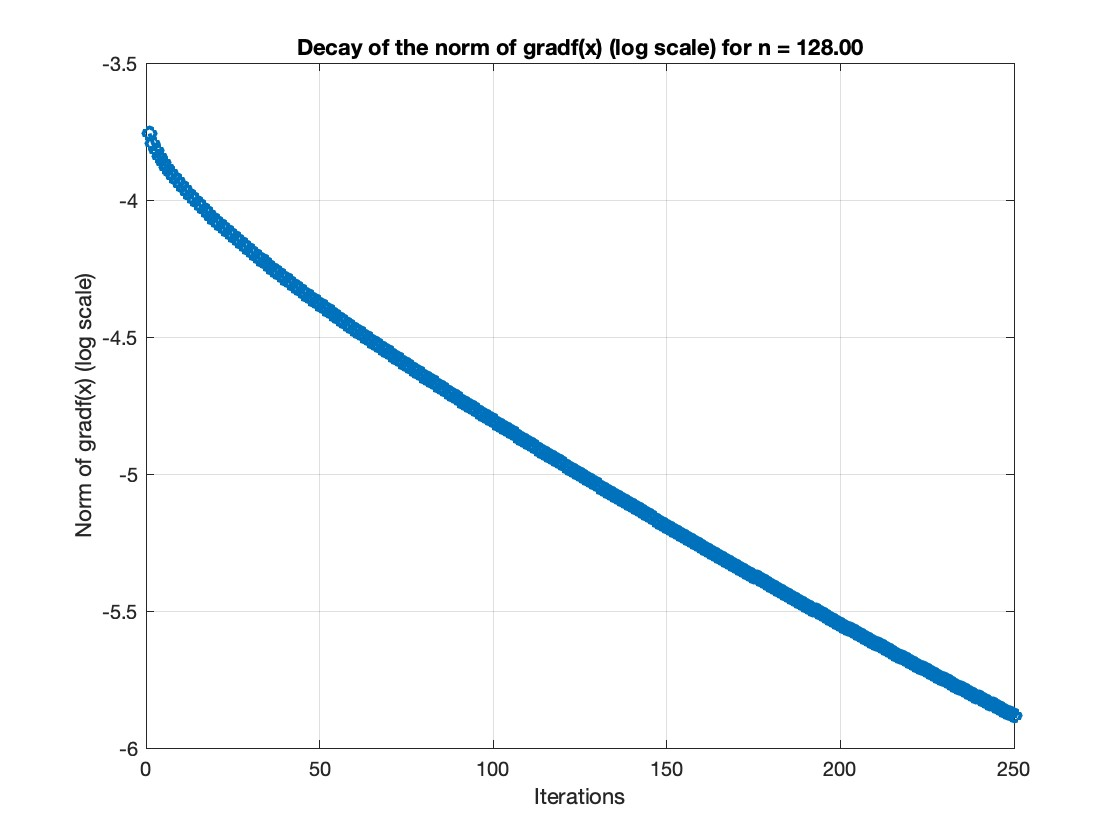
\includegraphics[width=\textwidth]{3g11.jpg}
%    \end{subfigure}
%    \caption{Experiment $11$ for $(3, 128)$}

%    \newpage

%    \begin{subfigure}[b]{0.45\textwidth}
%        \centering
%        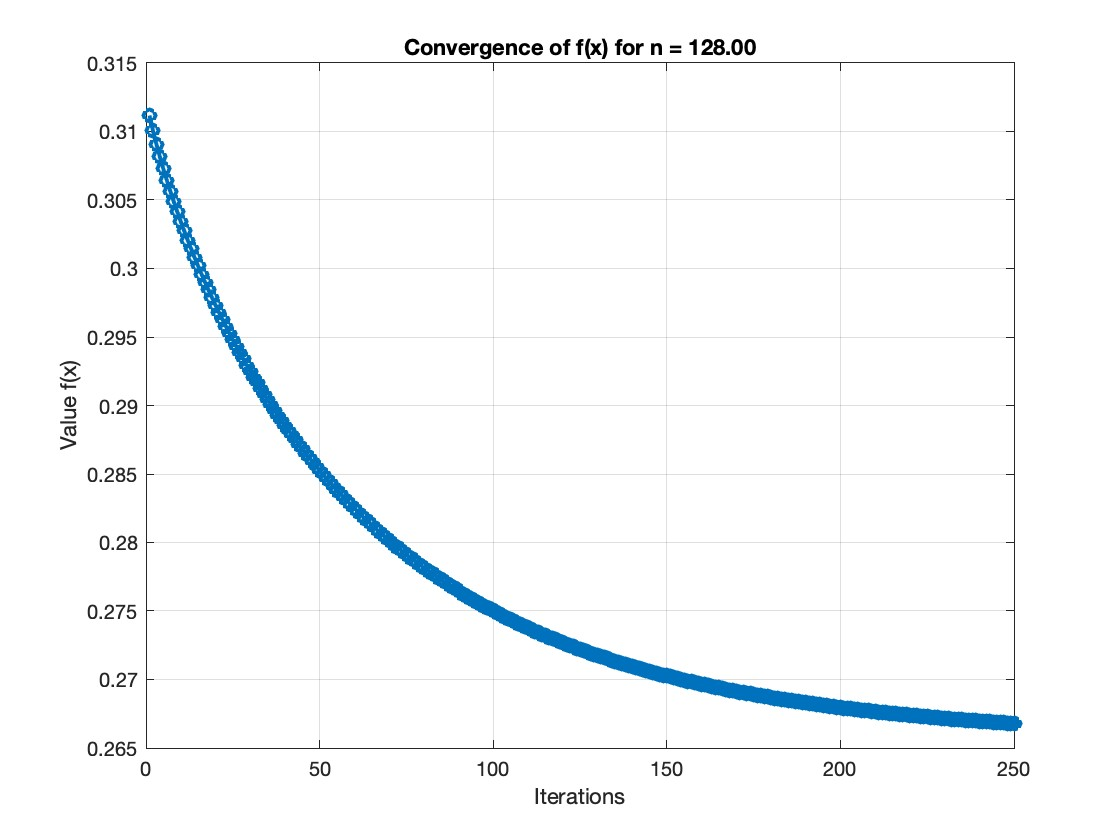
\includegraphics[width=\textwidth]{3f12.jpg}
%    \end{subfigure}
%    \begin{subfigure}[b]{0.45\textwidth}
%        \centering
%        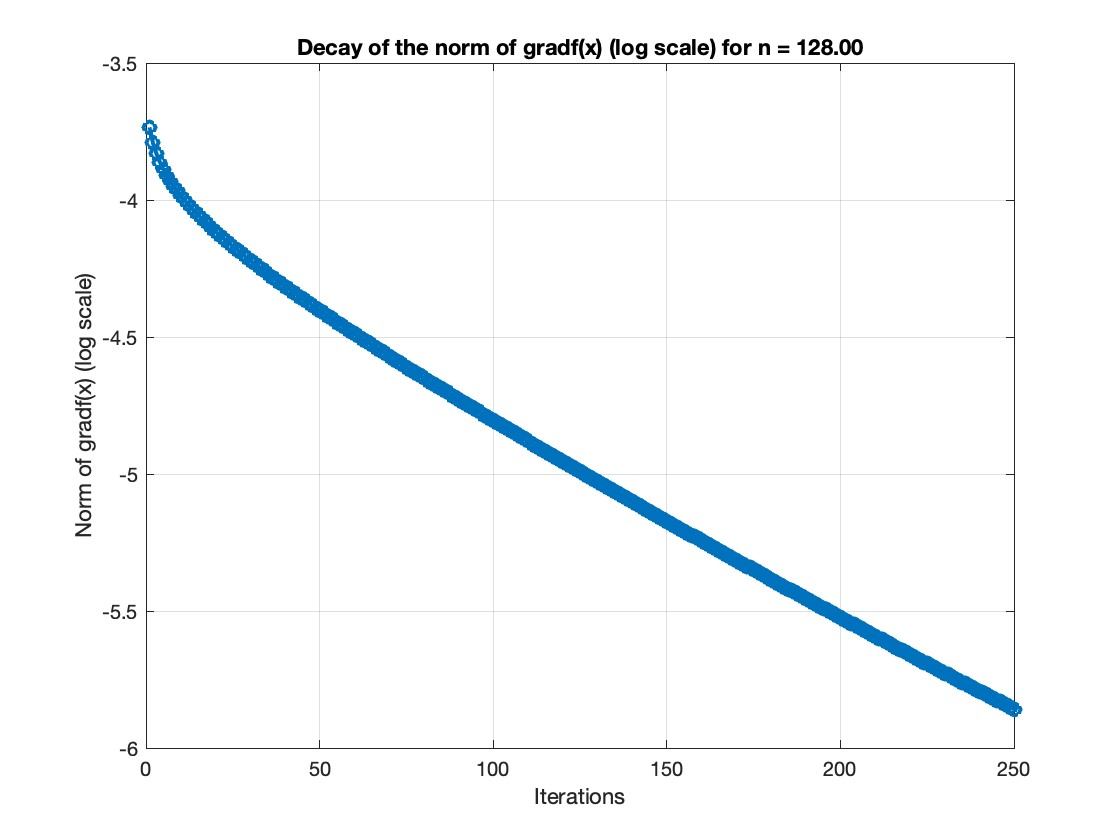
\includegraphics[width=\textwidth]{3g12.jpg}
%    \end{subfigure}
%    \caption{Experiment $12$ for $(3, 128)$}
%\end{figure}
%\begin{figure}
%    \centering
%    \begin{subfigure}[b]{0.45\textwidth}
%        \centering
%        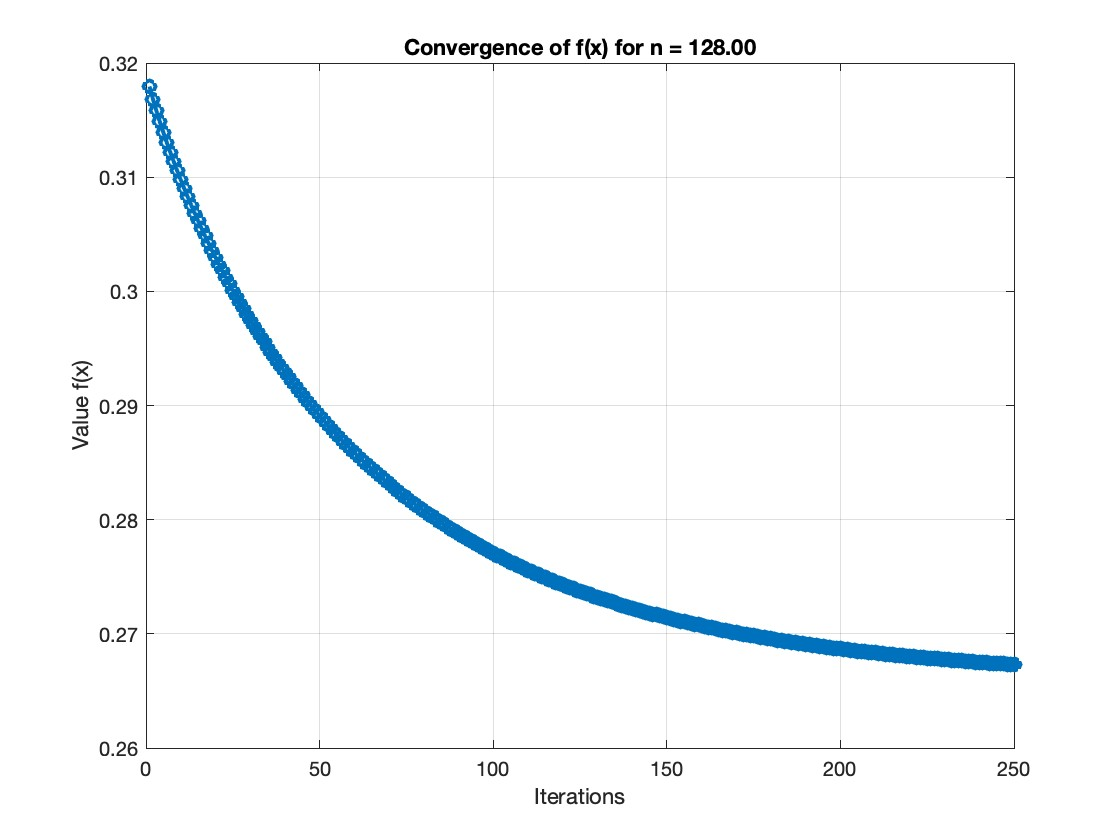
\includegraphics[width=\textwidth]{3f13.jpg}
%    \end{subfigure}
%    \begin{subfigure}[b]{0.45\textwidth}
%        \centering
%        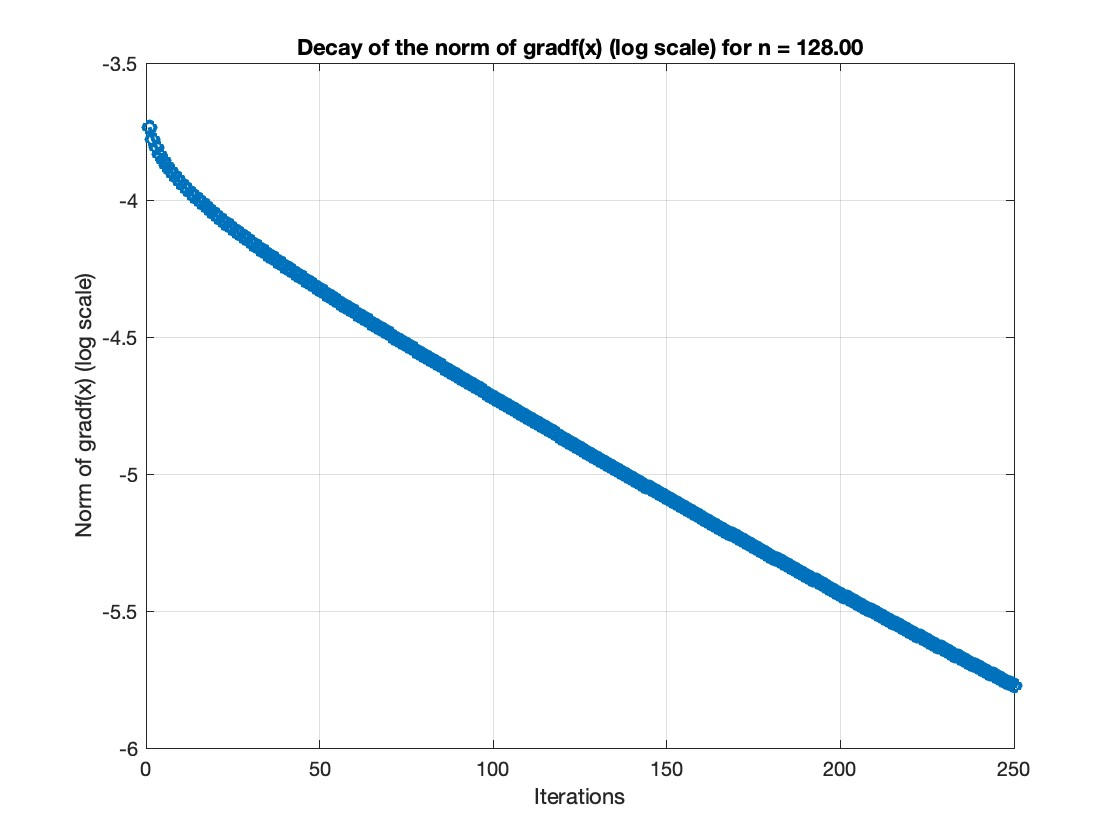
\includegraphics[width=\textwidth]{3g13.jpg}
%    \end{subfigure}
%    \caption{Experiment $13$ for $(3, 128)$}

%    \newpage

%    \begin{subfigure}[b]{0.45\textwidth}
%        \centering
%        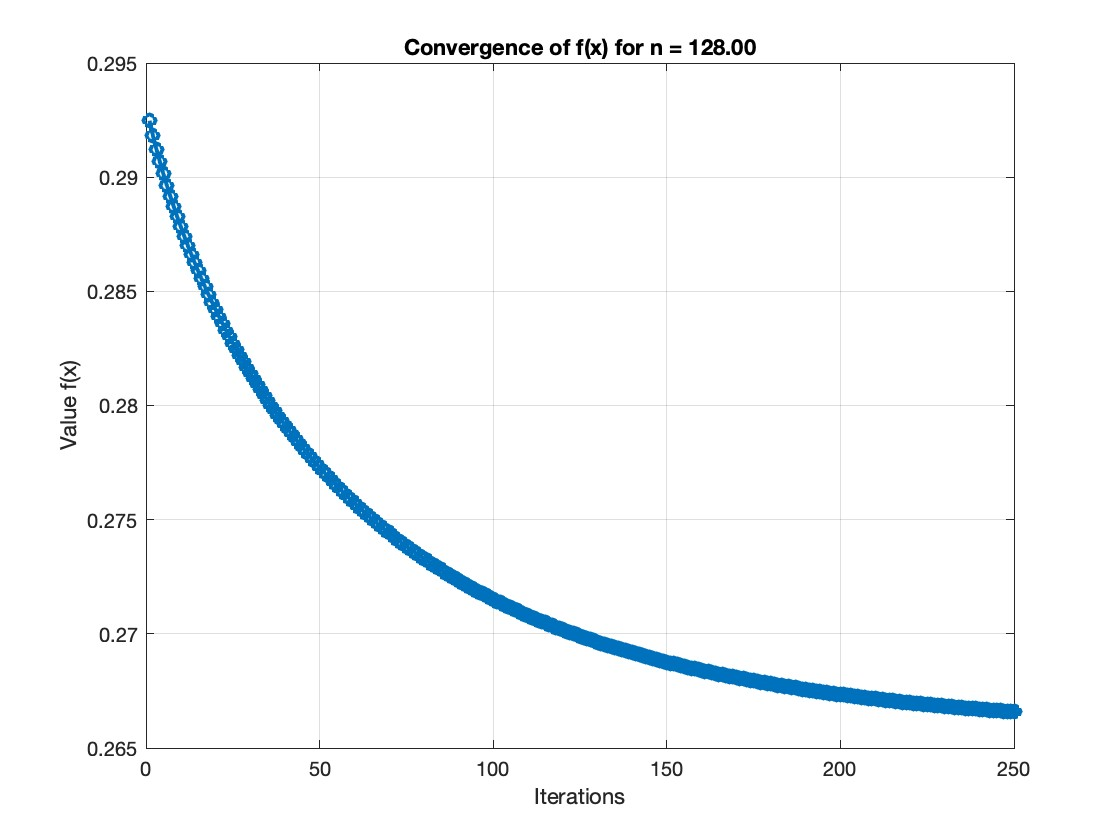
\includegraphics[width=\textwidth]{3f14.jpg}
%    \end{subfigure}
%    \begin{subfigure}[b]{0.45\textwidth}
%        \centering
%        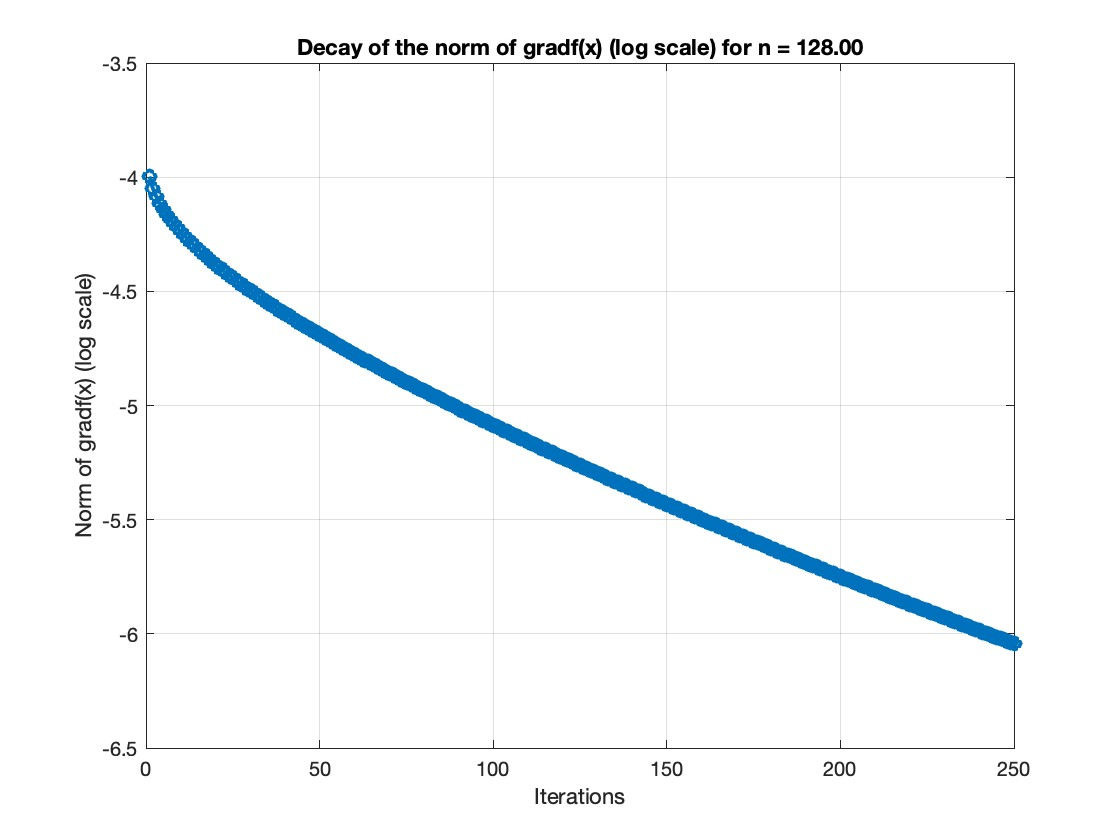
\includegraphics[width=\textwidth]{3g14.jpg}
%    \end{subfigure}
%    \caption{Experiment $14$ for $(3, 128)$}

%    \newpage

%    \begin{subfigure}[b]{0.45\textwidth}
%        \centering
%        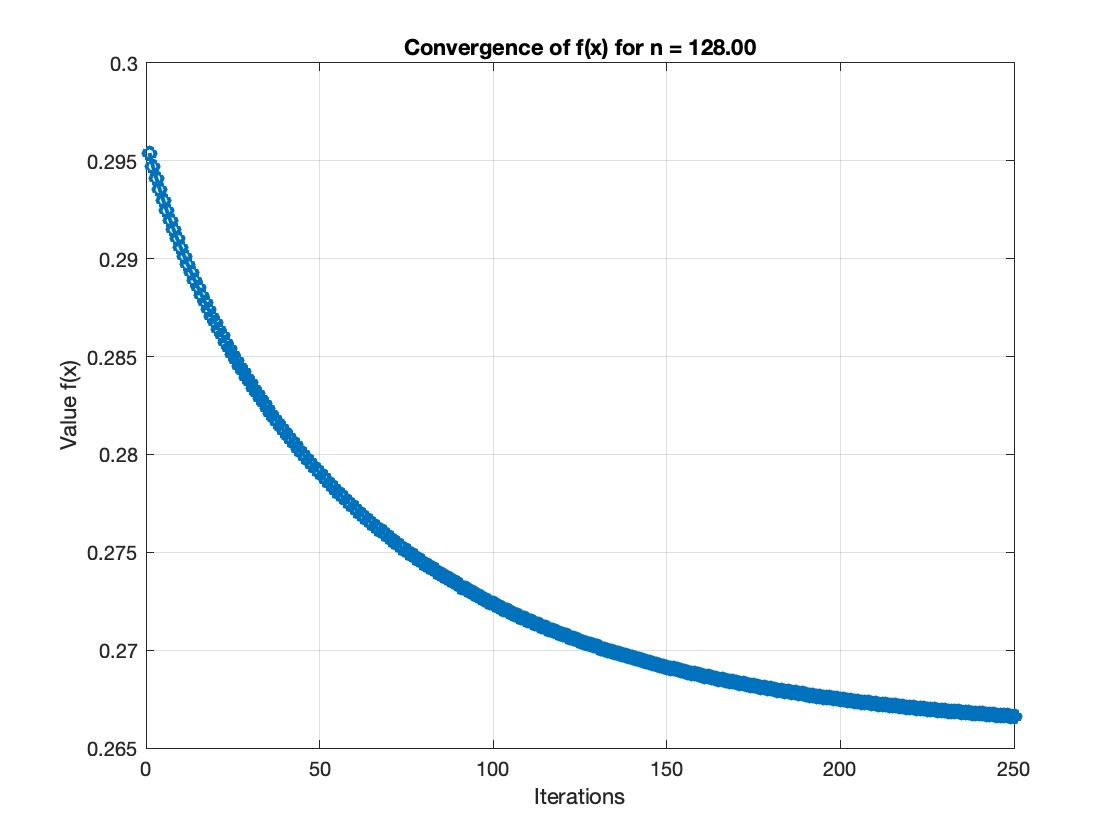
\includegraphics[width=\textwidth]{3f15.jpg}
%    \end{subfigure}
%    \begin{subfigure}[b]{0.45\textwidth}
%        \centering
%        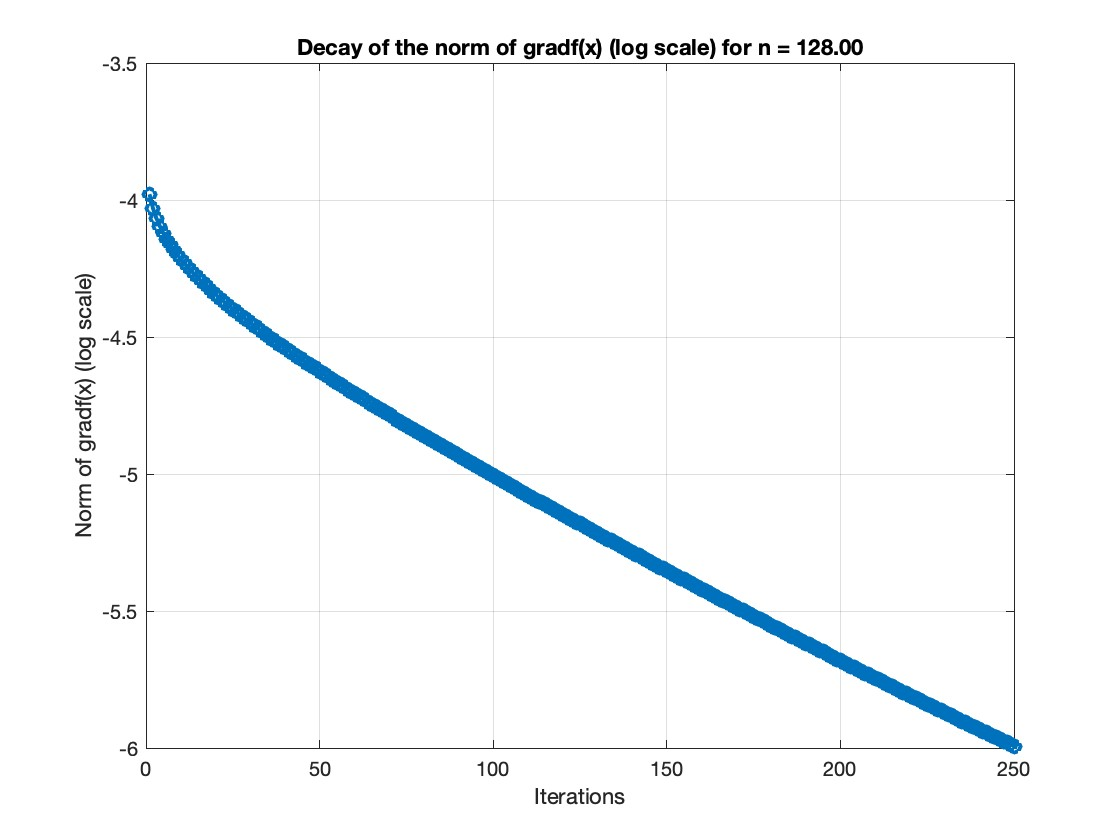
\includegraphics[width=\textwidth]{3g15.jpg}
%    \end{subfigure}
%    \caption{Experiment $15$ for $(3, 128)$}

%    \newpage

%    \begin{subfigure}[b]{0.45\textwidth}
%        \centering
%        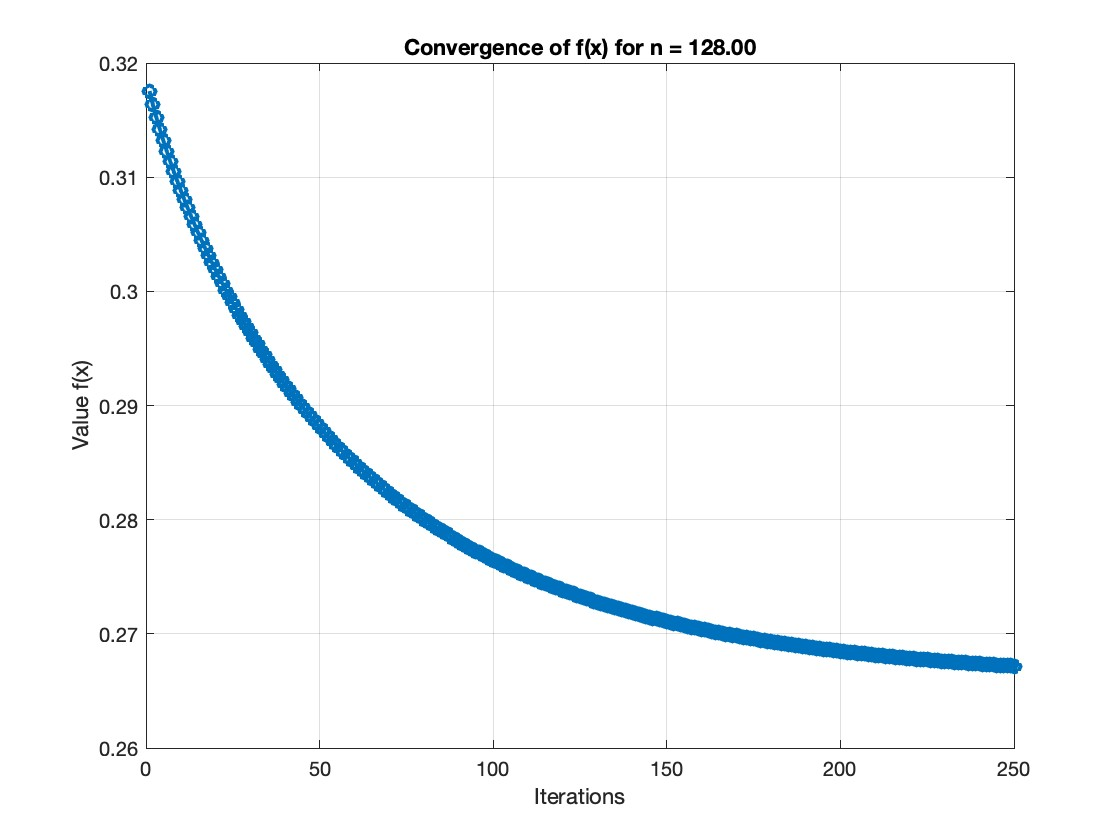
\includegraphics[width=\textwidth]{3f16.jpg}
%    \end{subfigure}
%    \begin{subfigure}[b]{0.45\textwidth}
%        \centering
%        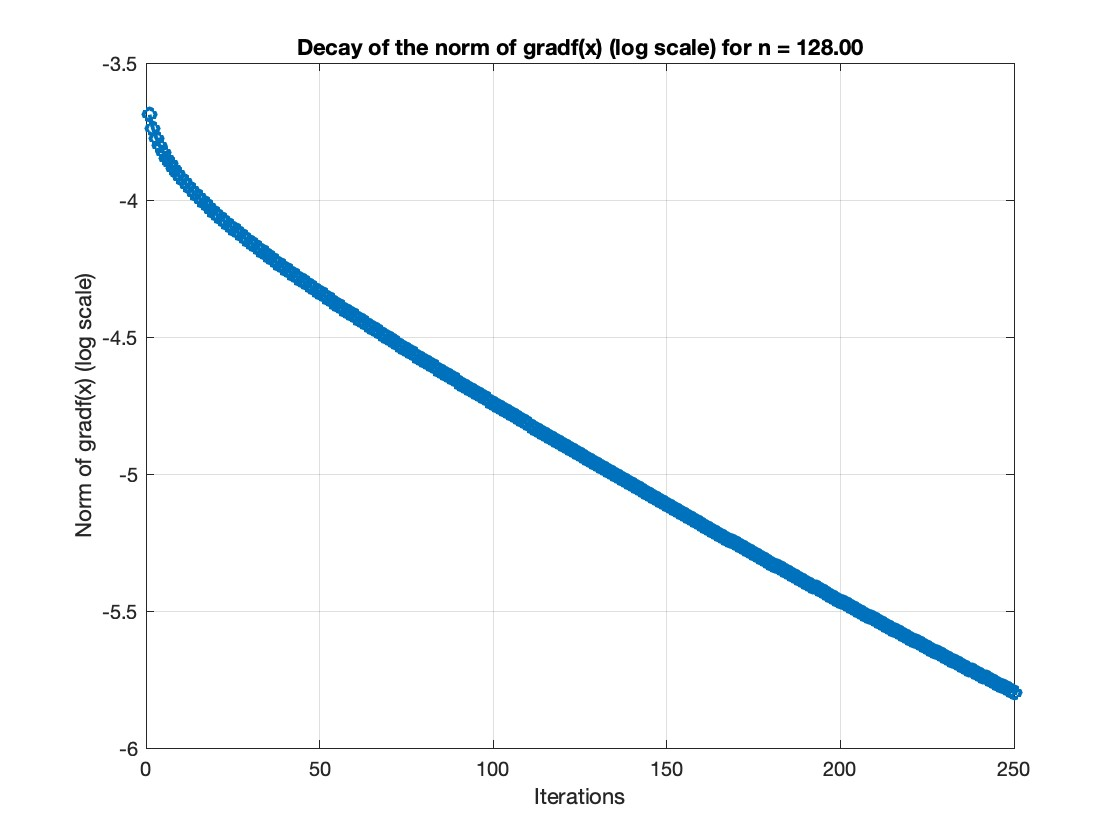
\includegraphics[width=\textwidth]{3g16.jpg}
%    \end{subfigure}
%    \caption{Experiment $16$ for $(3, 128)$}
%\end{figure}
%\begin{figure}
%    \centering
%    \begin{subfigure}[b]{0.45\textwidth}
%        \centering
%        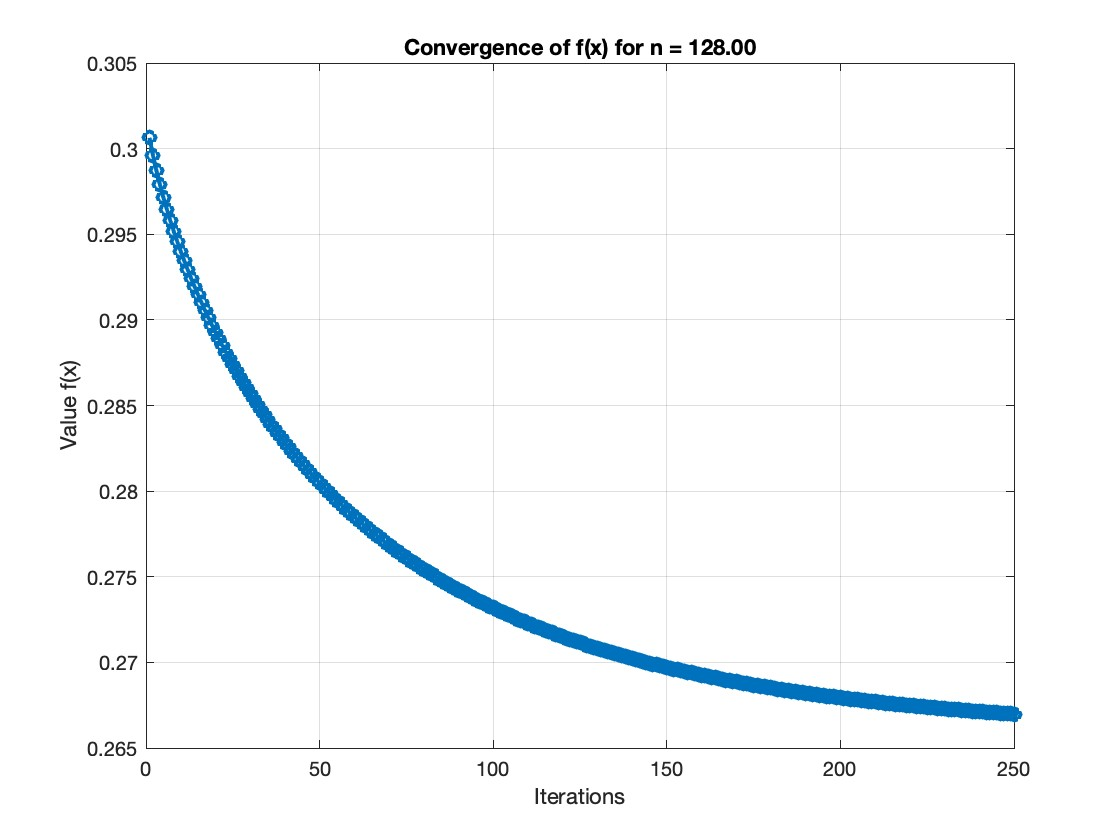
\includegraphics[width=\textwidth]{3f17.jpg}
%    \end{subfigure}
%    \begin{subfigure}[b]{0.45\textwidth}
%        \centering
%        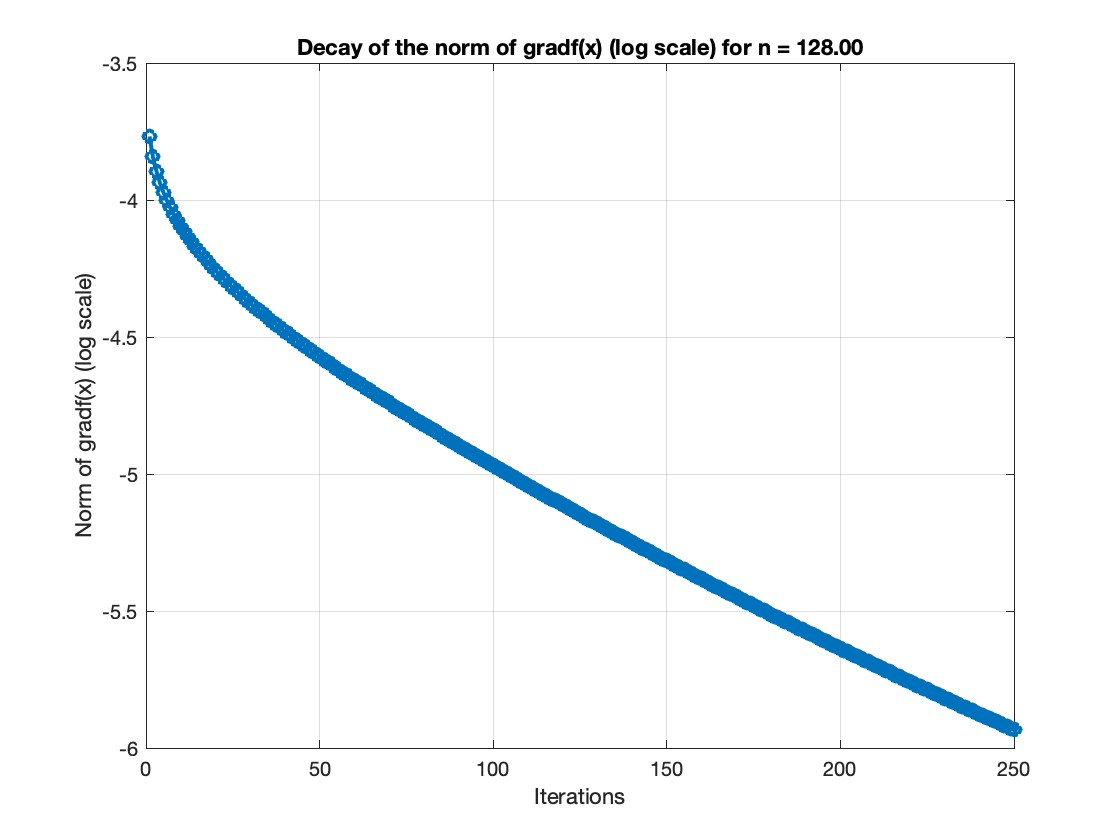
\includegraphics[width=\textwidth]{3g17.jpg}
%    \end{subfigure}
%    \caption{Experiment $17$ for $(3, 128)$}

%    \newpage

%    \begin{subfigure}[b]{0.45\textwidth}
%        \centering
%        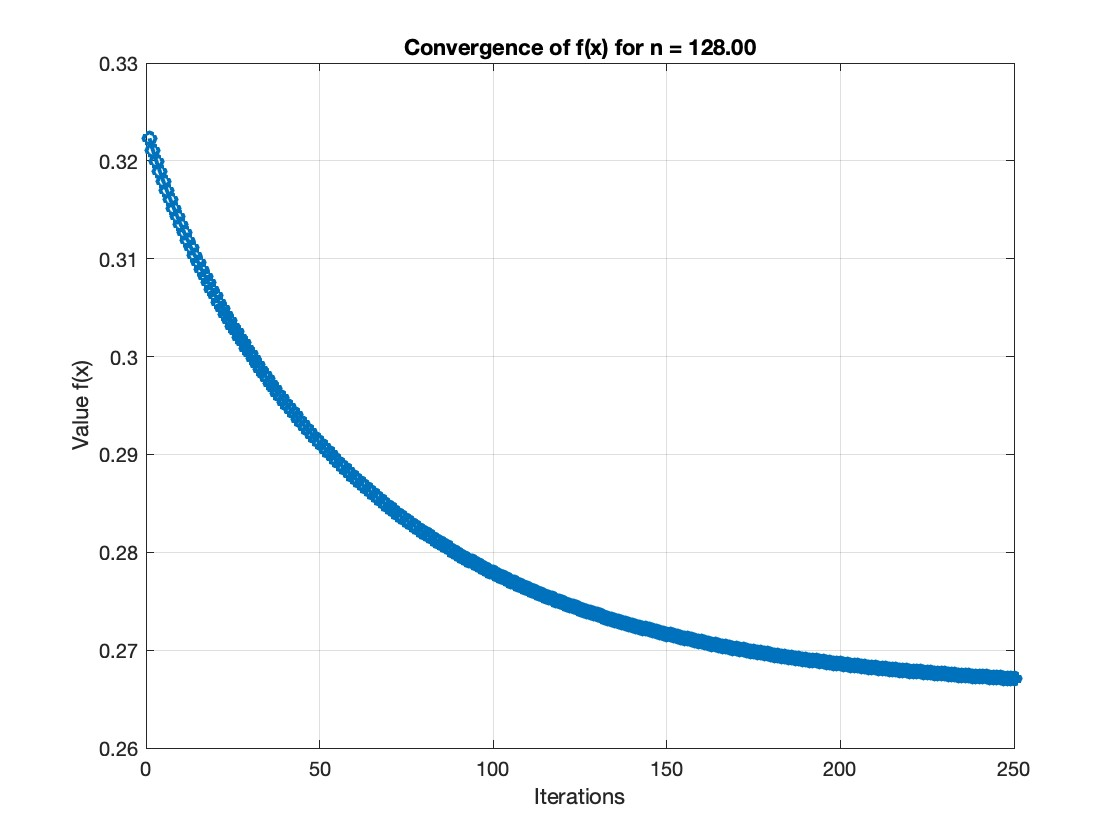
\includegraphics[width=\textwidth]{3f18.jpg}
%    \end{subfigure}
%    \begin{subfigure}[b]{0.45\textwidth}
%        \centering
%        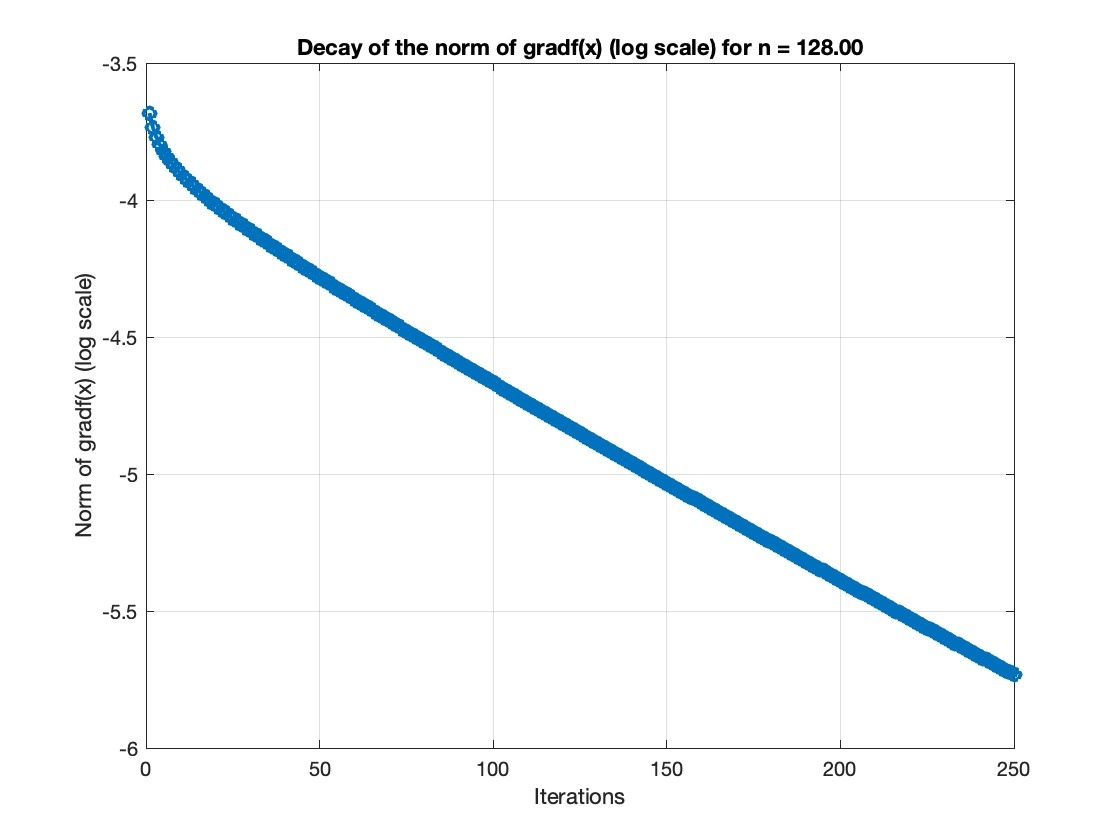
\includegraphics[width=\textwidth]{3g18.jpg}
%    \end{subfigure}
%    \caption{Experiment $18$ for $(3, 128)$}

%    \newpage

%    \begin{subfigure}[b]{0.45\textwidth}
%        \centering
%        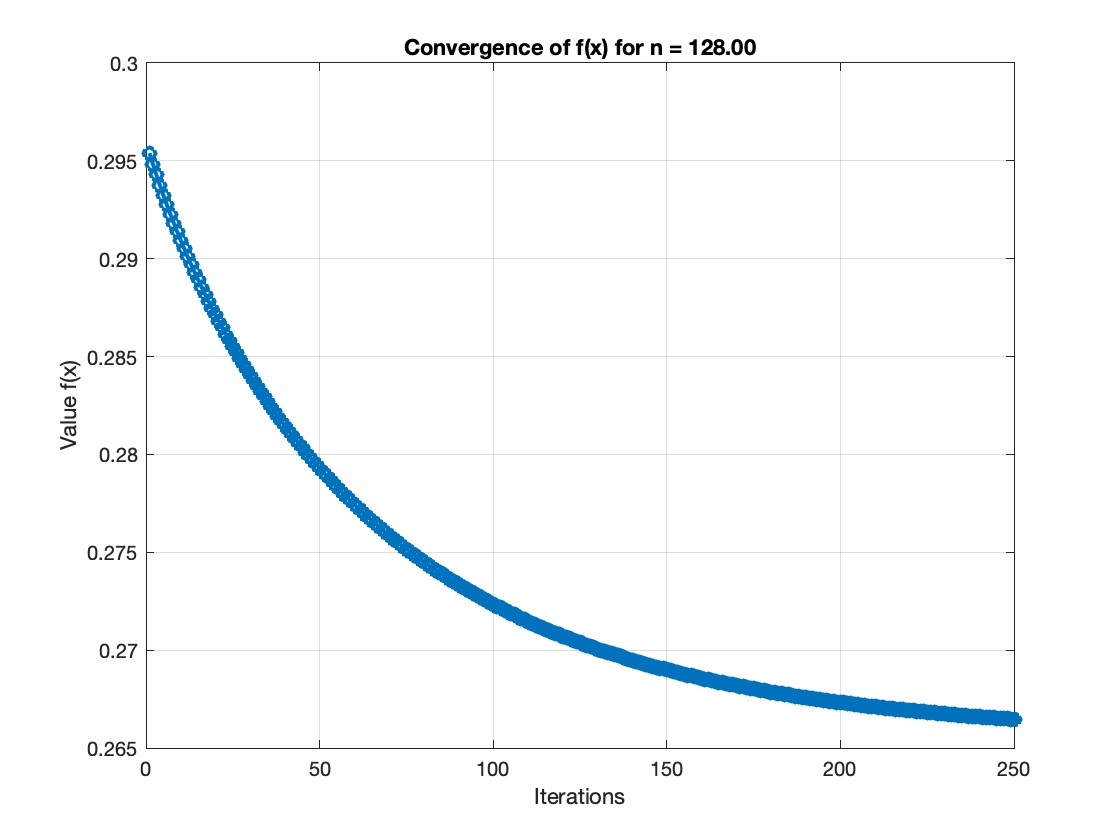
\includegraphics[width=\textwidth]{3f19.jpg}
%    \end{subfigure}
%    \begin{subfigure}[b]{0.45\textwidth}
%        \centering
%        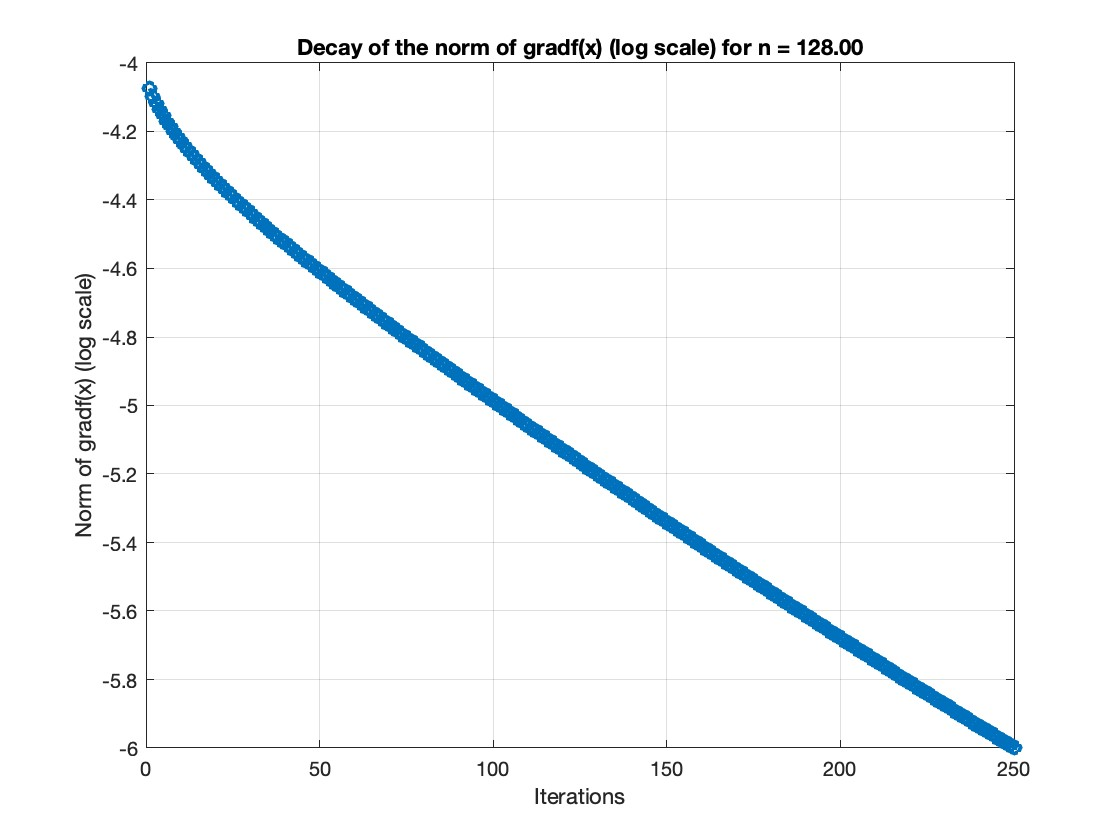
\includegraphics[width=\textwidth]{3g19.jpg}
%    \end{subfigure}
%    \caption{Experiment $19$ for $(3, 128)$}

%    \newpage

%    \begin{subfigure}[b]{0.45\textwidth}
%        \centering
%        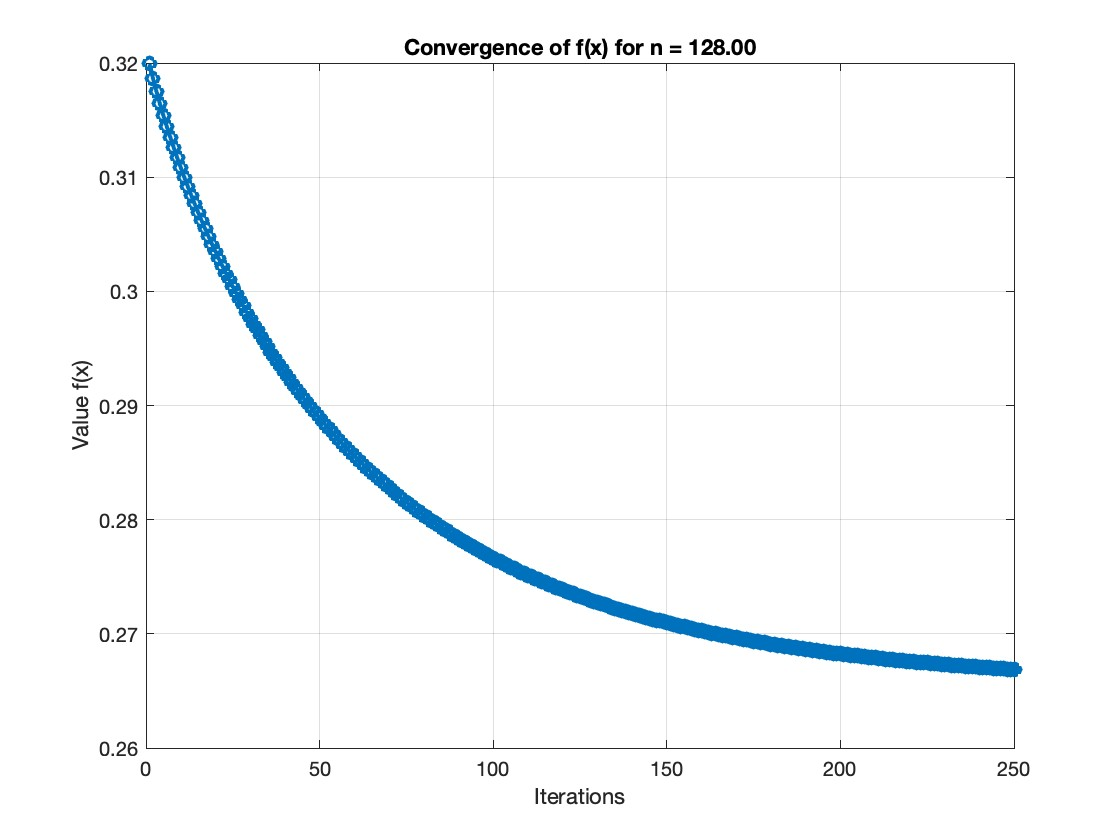
\includegraphics[width=\textwidth]{3f20.jpg}
%    \end{subfigure}
%    \begin{subfigure}[b]{0.45\textwidth}
%        \centering
%        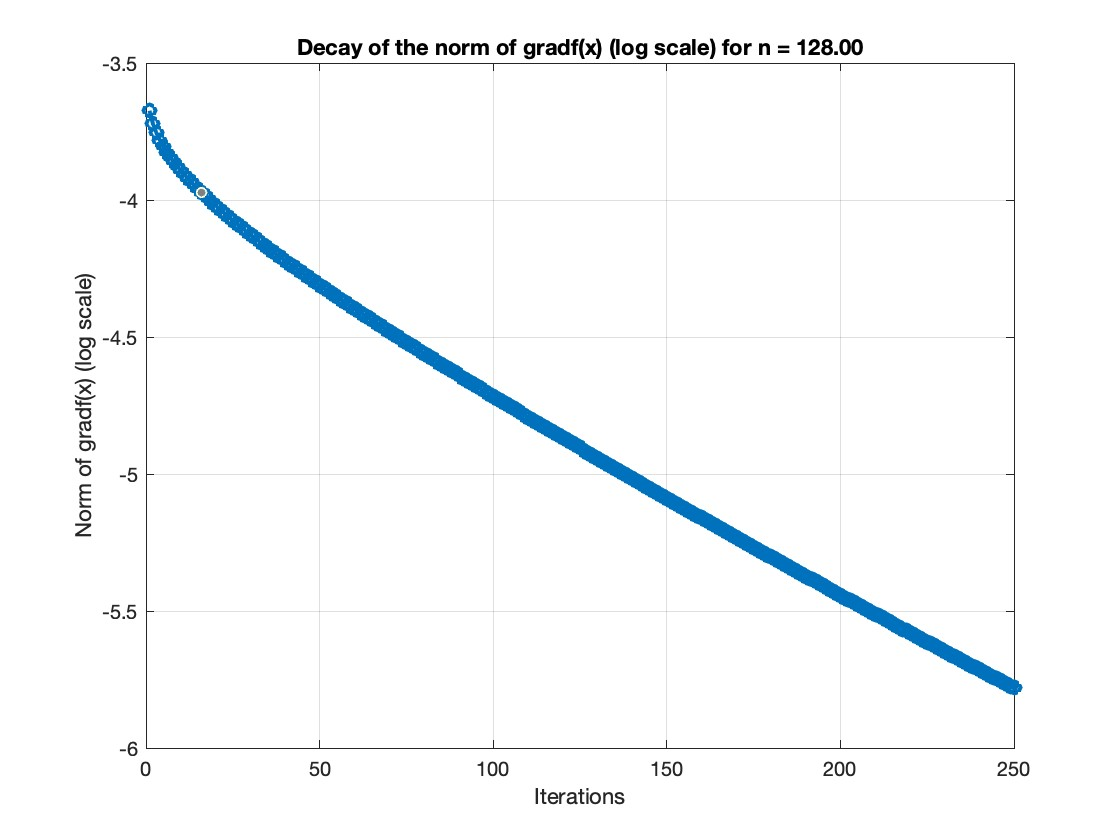
\includegraphics[width=\textwidth]{3g20.jpg}
%    \end{subfigure}
%    \caption{Experiment $20$ for $(3, 128)$}
%\end{figure}
%\begin{figure}
%    \centering
%    \begin{subfigure}[b]{0.45\textwidth}
%        \centering
%        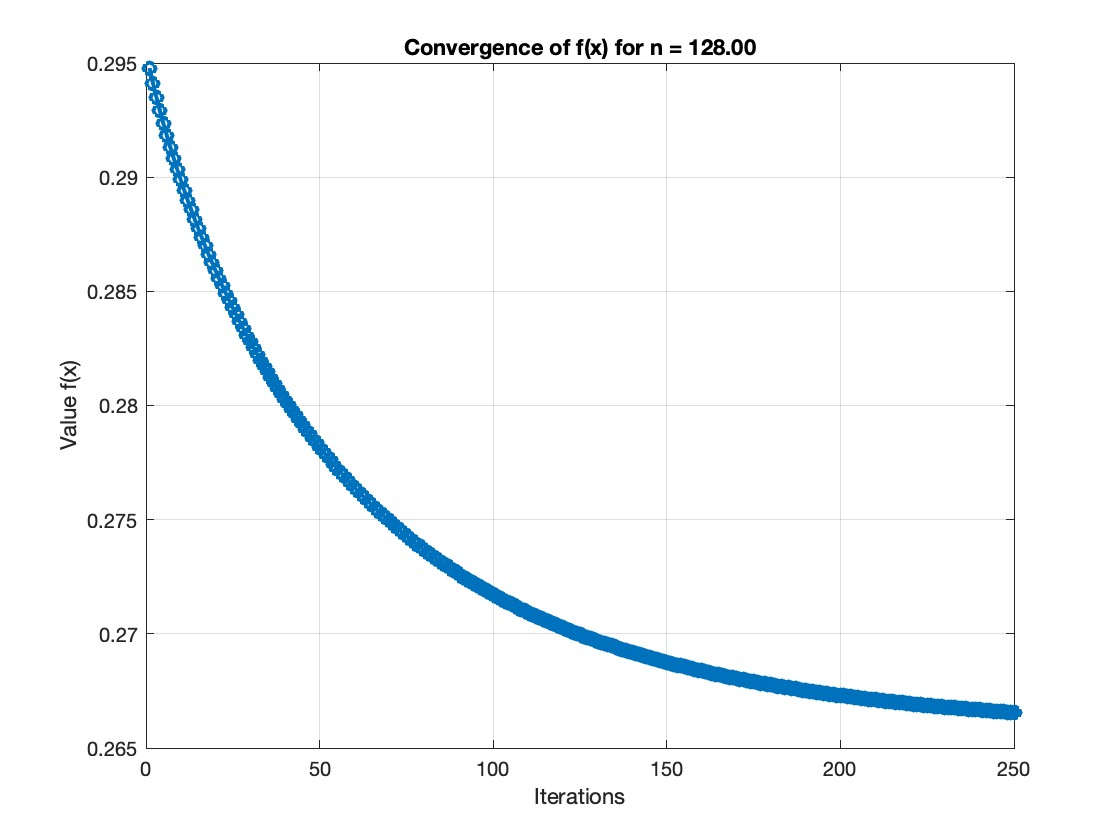
\includegraphics[width=\textwidth]{3f21.jpg}
%    \end{subfigure}
%    \begin{subfigure}[b]{0.45\textwidth}
%        \centering
%        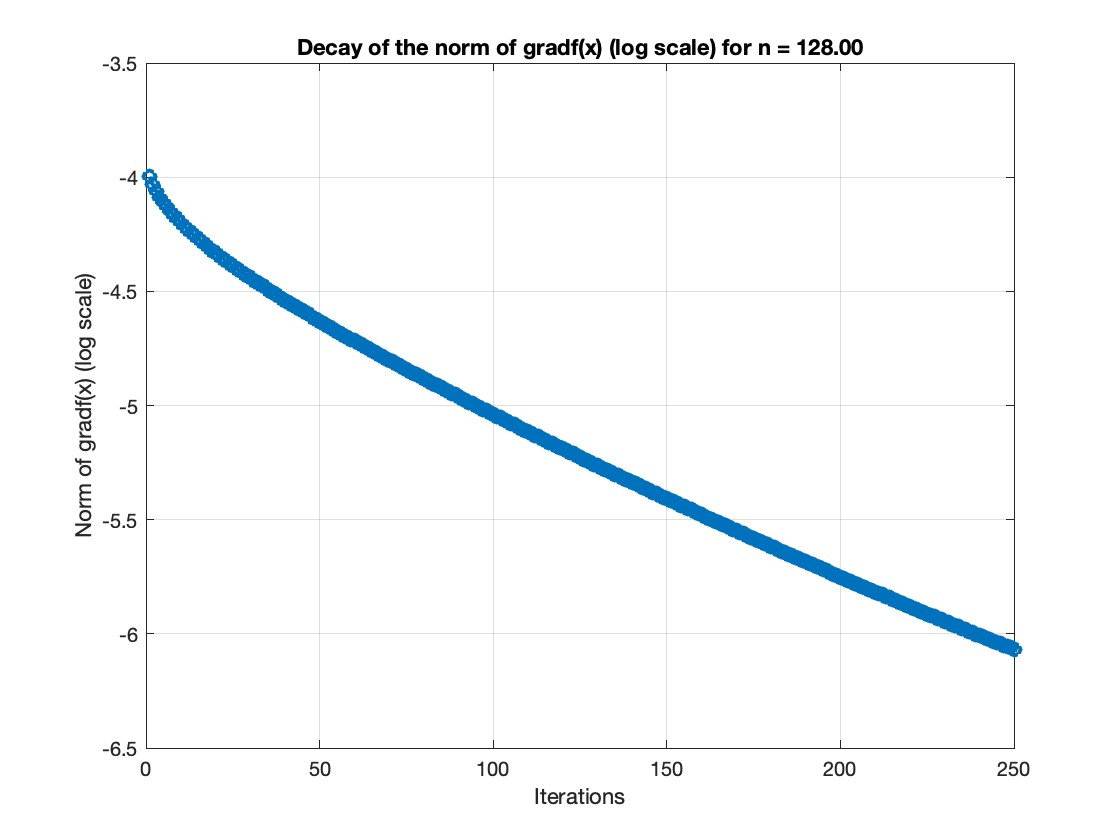
\includegraphics[width=\textwidth]{3g21.jpg}
%    \end{subfigure}
%    \caption{Experiment $21$ for $(3, 128)$}

%    \newpage

%    \begin{subfigure}[b]{0.45\textwidth}
%        \centering
%        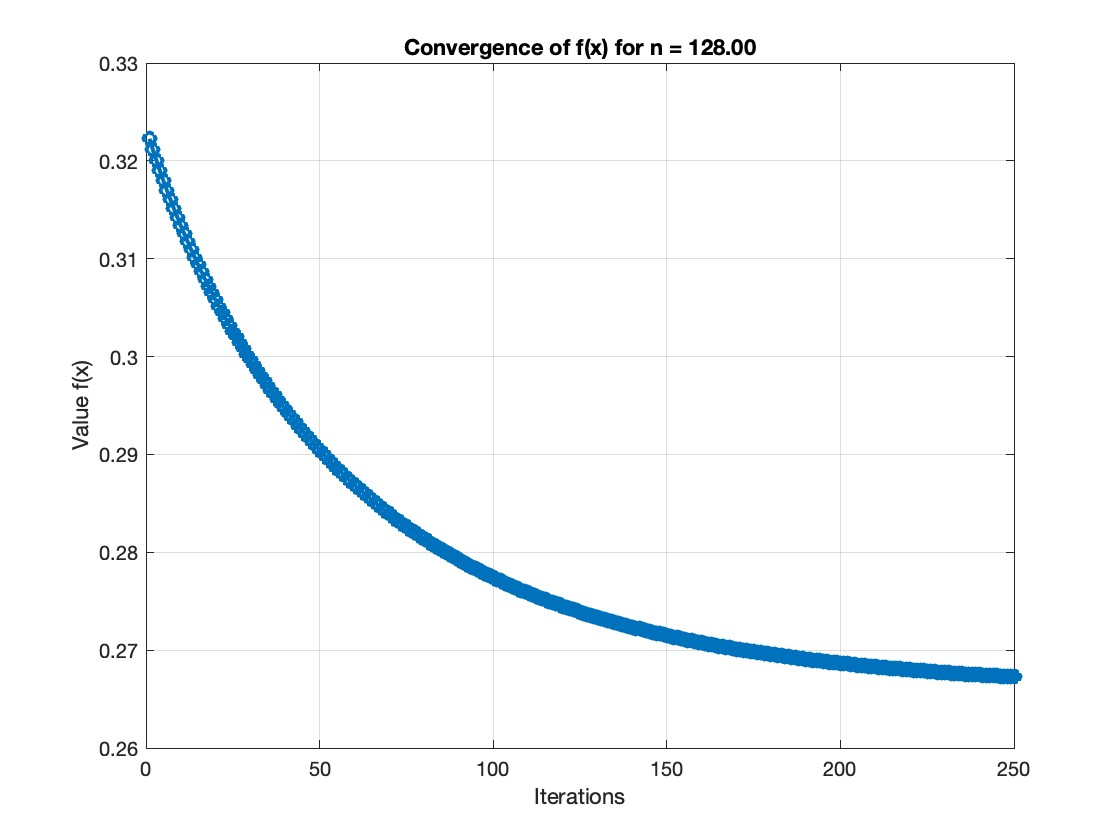
\includegraphics[width=\textwidth]{3f22.jpg}
%    \end{subfigure}
%    \begin{subfigure}[b]{0.45\textwidth}
%        \centering
%        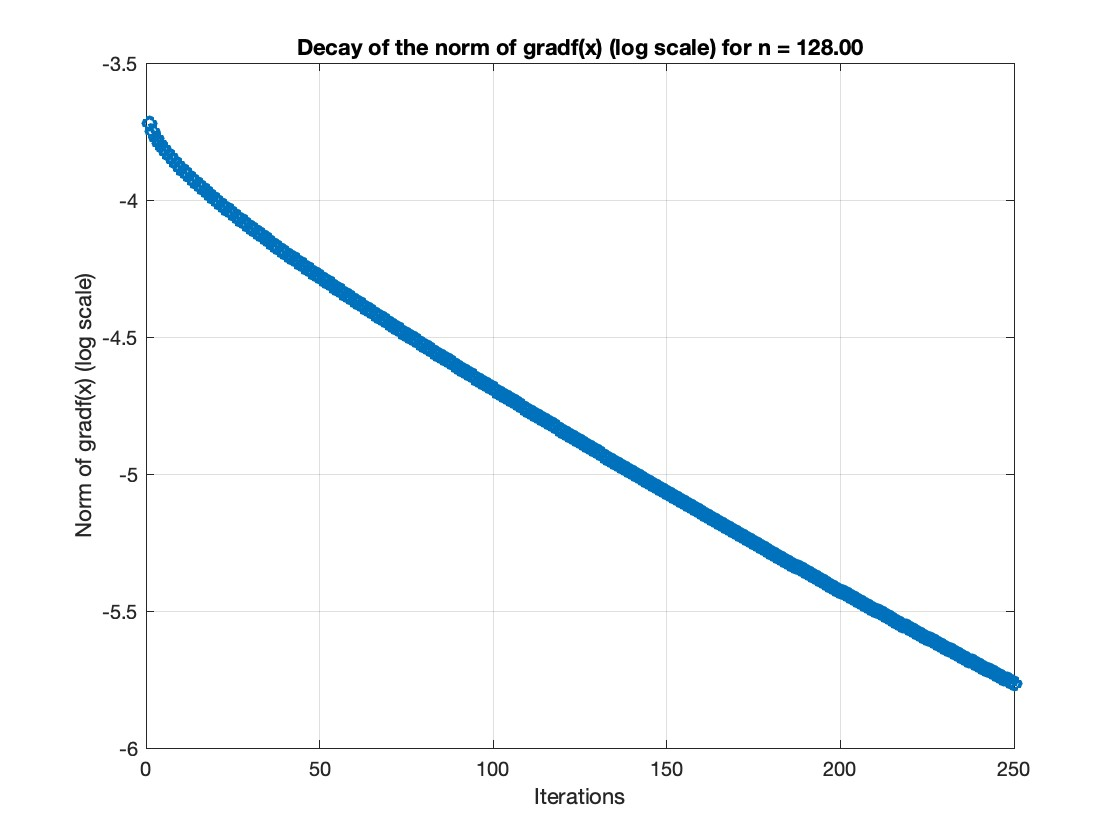
\includegraphics[width=\textwidth]{3g22.jpg}
%    \end{subfigure}
%    \caption{Experiment $22$ for $(3, 128)$}

%    \newpage

%    \begin{subfigure}[b]{0.45\textwidth}
%        \centering
%        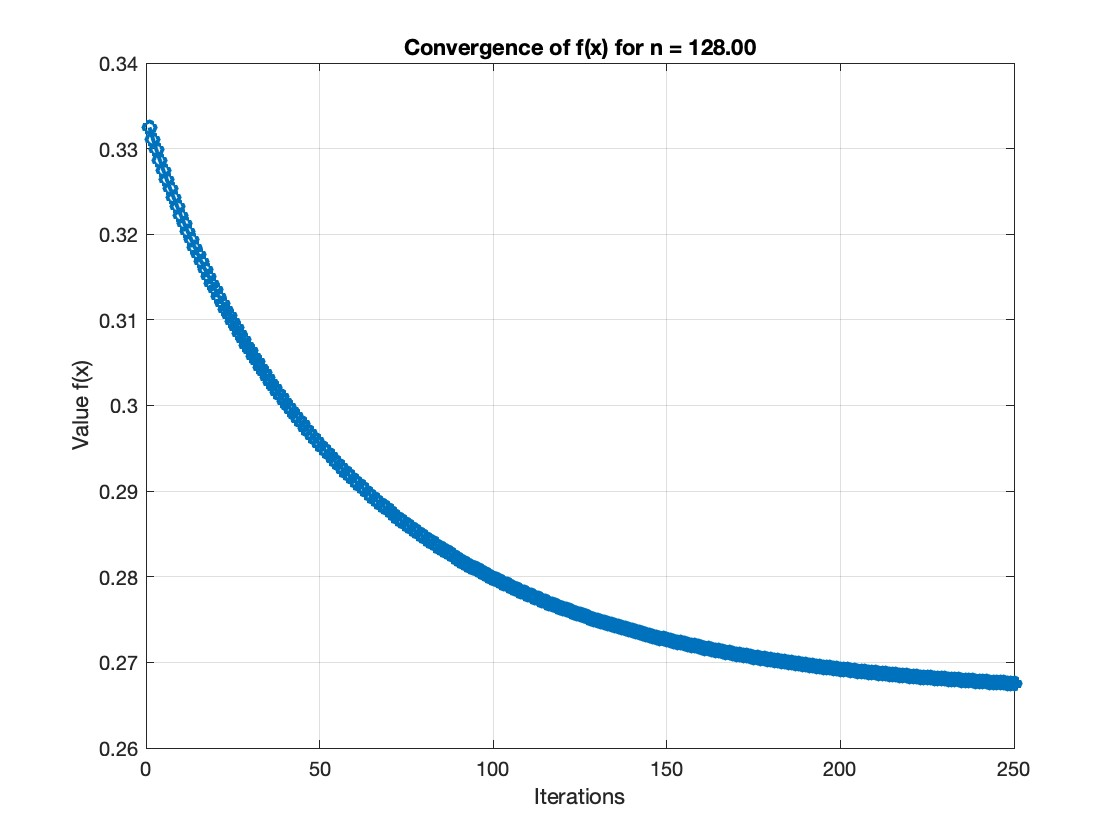
\includegraphics[width=\textwidth]{3f23.jpg}
%    \end{subfigure}
%    \begin{subfigure}[b]{0.45\textwidth}
%        \centering
%        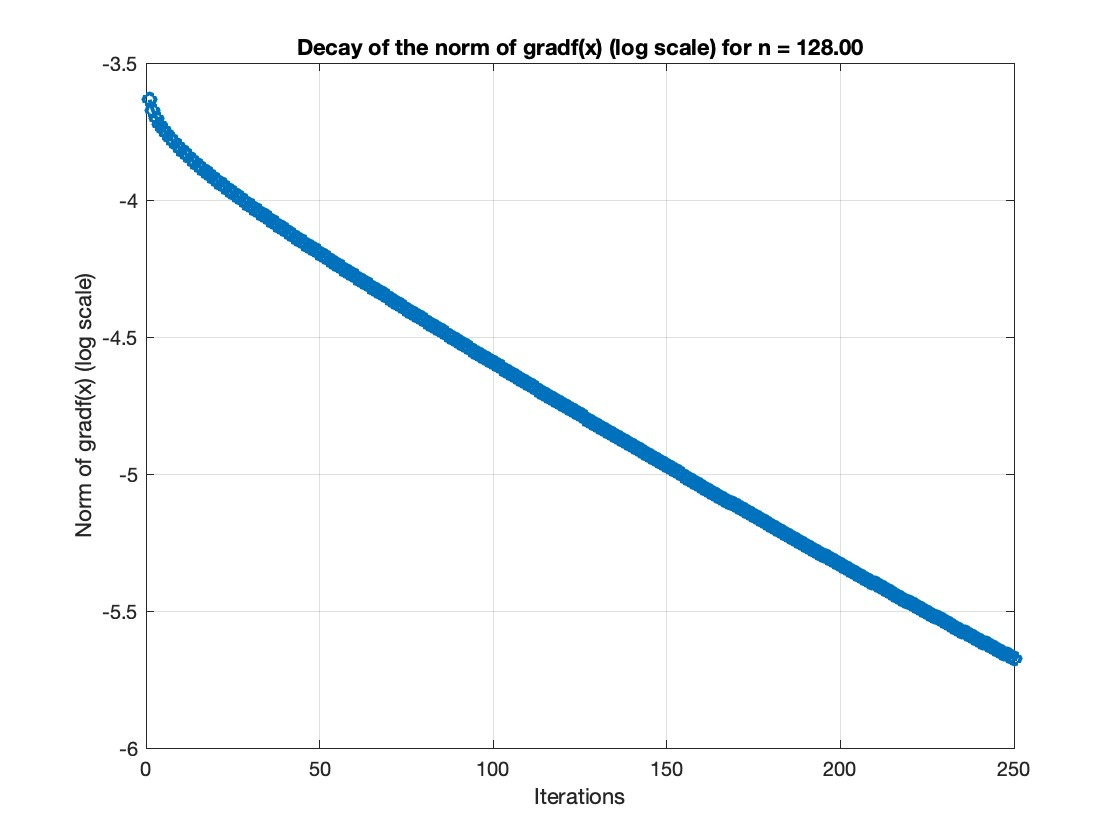
\includegraphics[width=\textwidth]{3g23.jpg}
%    \end{subfigure}
%    \caption{Experiment $23$ for $(3, 128)$}

%    \newpage

%    \begin{subfigure}[b]{0.45\textwidth}
%        \centering
%        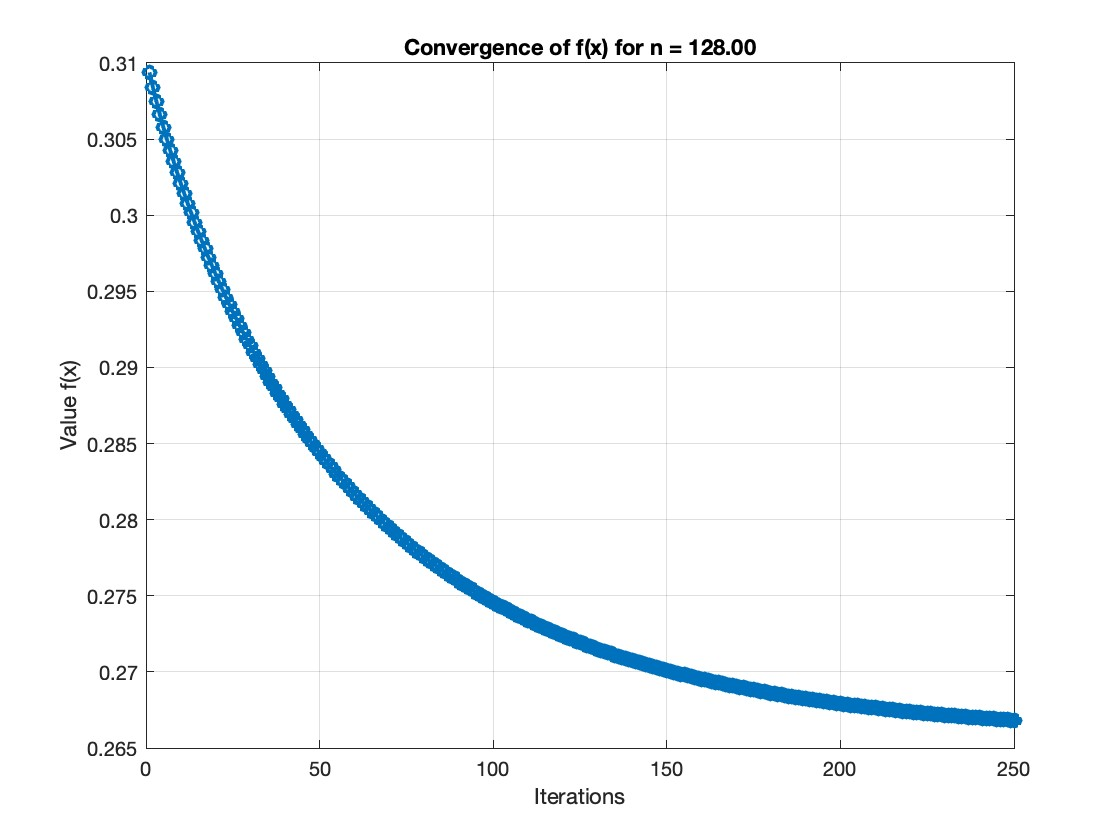
\includegraphics[width=\textwidth]{3f24.jpg}
%    \end{subfigure}
%    \begin{subfigure}[b]{0.45\textwidth}
%        \centering
%        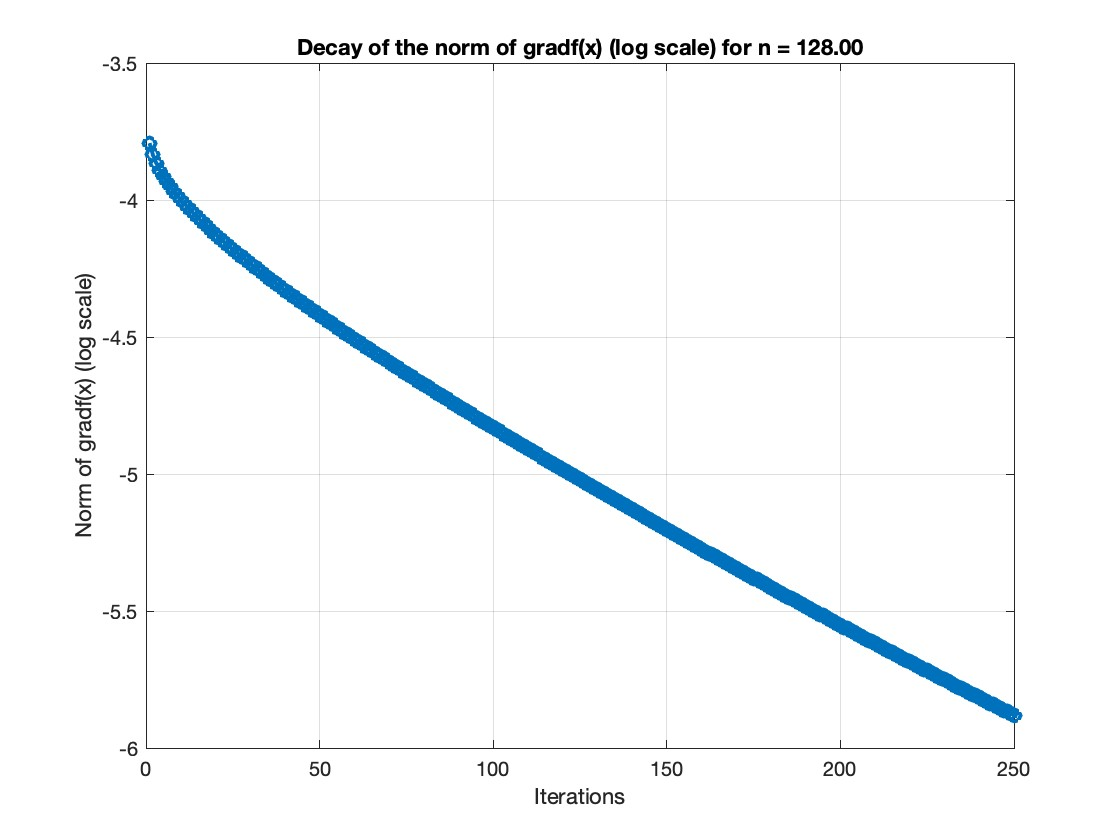
\includegraphics[width=\textwidth]{3g24.jpg}
%    \end{subfigure}
%    \caption{Experiment $24$ for $(3, 128)$}
%\end{figure}
%\begin{figure}
%    \centering
%    \begin{subfigure}[b]{0.45\textwidth}
%        \centering
%        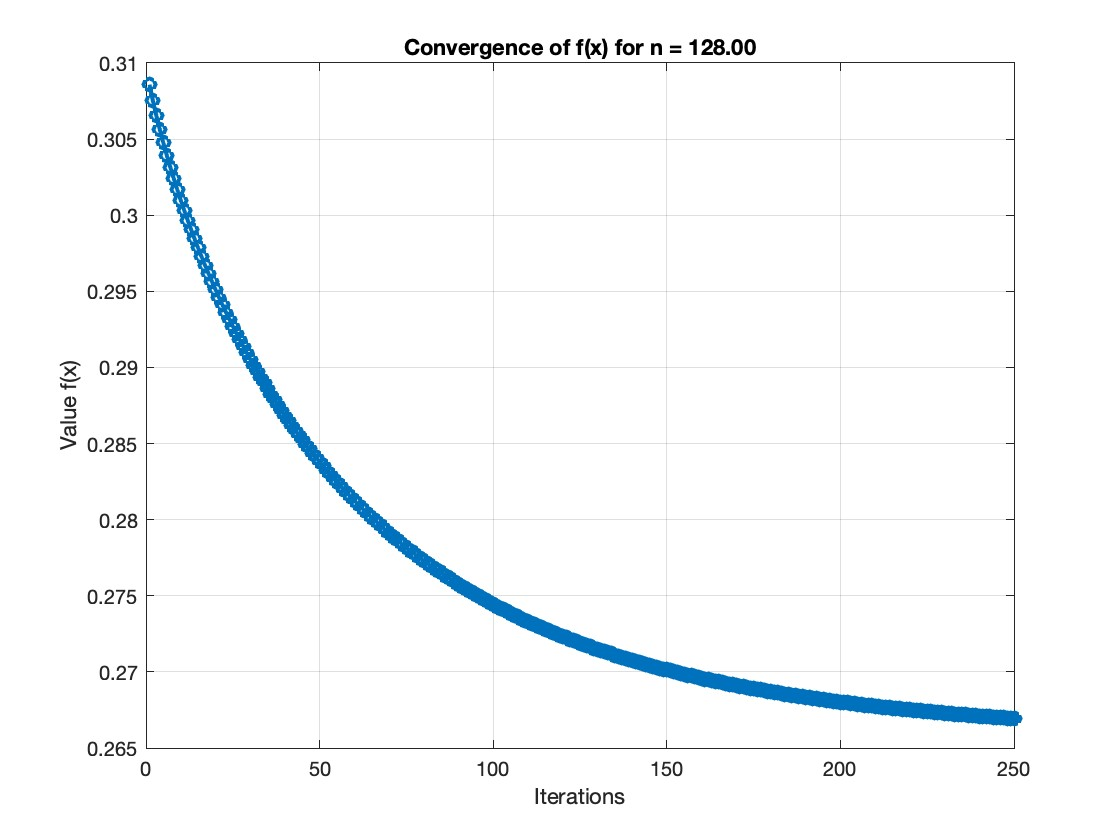
\includegraphics[width=\textwidth]{3f25.jpg}
%    \end{subfigure}
%    \begin{subfigure}[b]{0.45\textwidth}
%        \centering
%        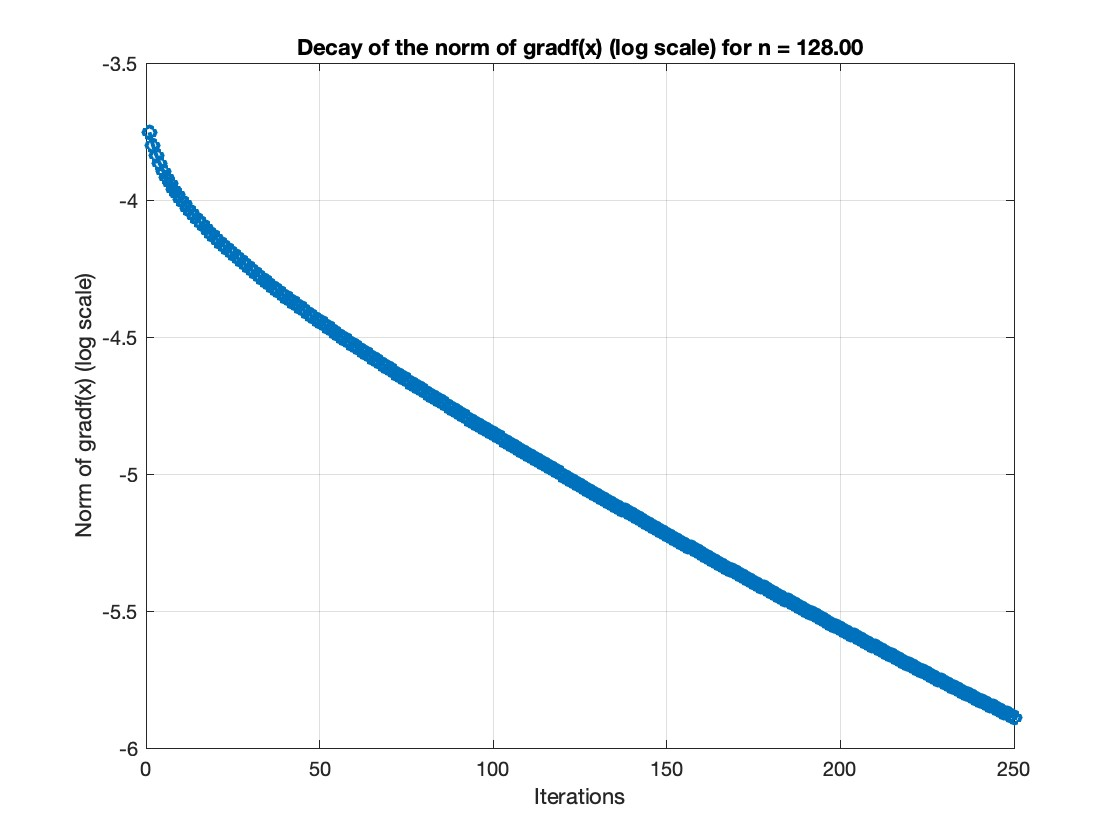
\includegraphics[width=\textwidth]{3g25.jpg}
%    \end{subfigure}
%    \caption{Experiment $25$ for $(3, 128)$}

%    \newpage

%    \begin{subfigure}[b]{0.45\textwidth}
%        \centering
%        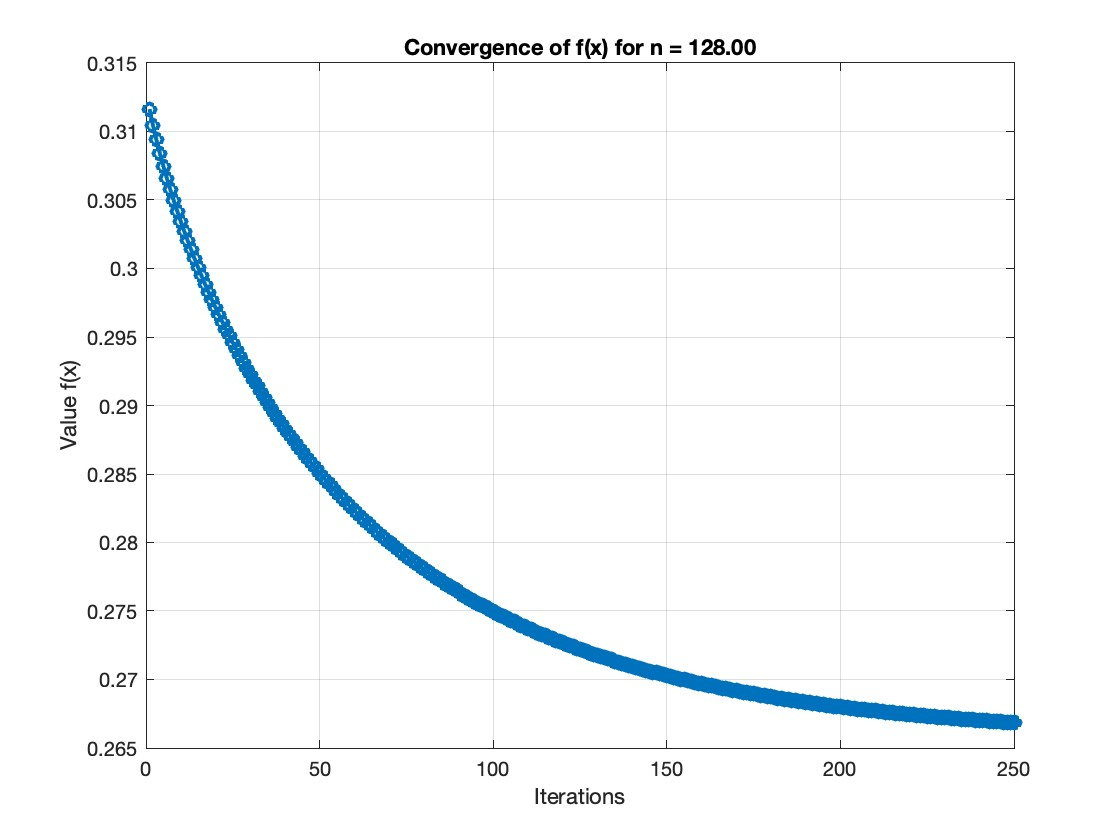
\includegraphics[width=\textwidth]{3f26.jpg}
%    \end{subfigure}
%    \begin{subfigure}[b]{0.45\textwidth}
%        \centering
%        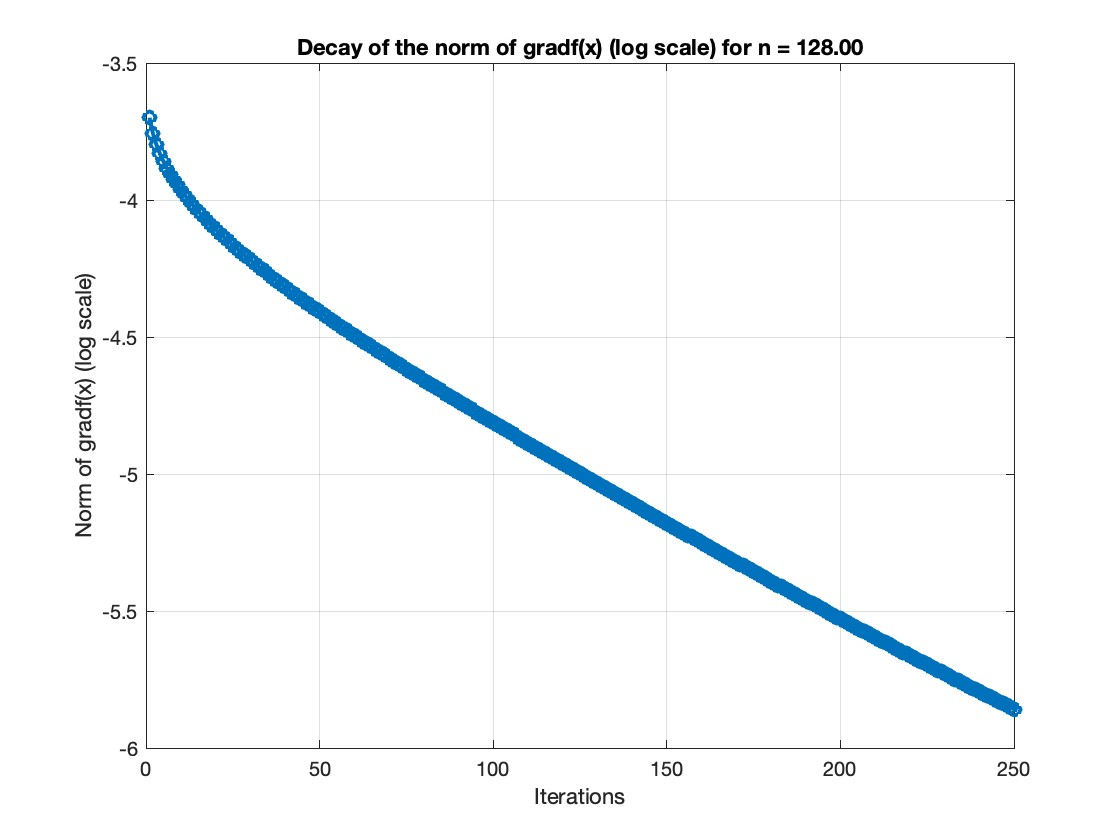
\includegraphics[width=\textwidth]{3g26.jpg}
%    \end{subfigure}
%    \caption{Experiment $26$ for $(3, 128)$}

%    \newpage

%    \begin{subfigure}[b]{0.45\textwidth}
%        \centering
%        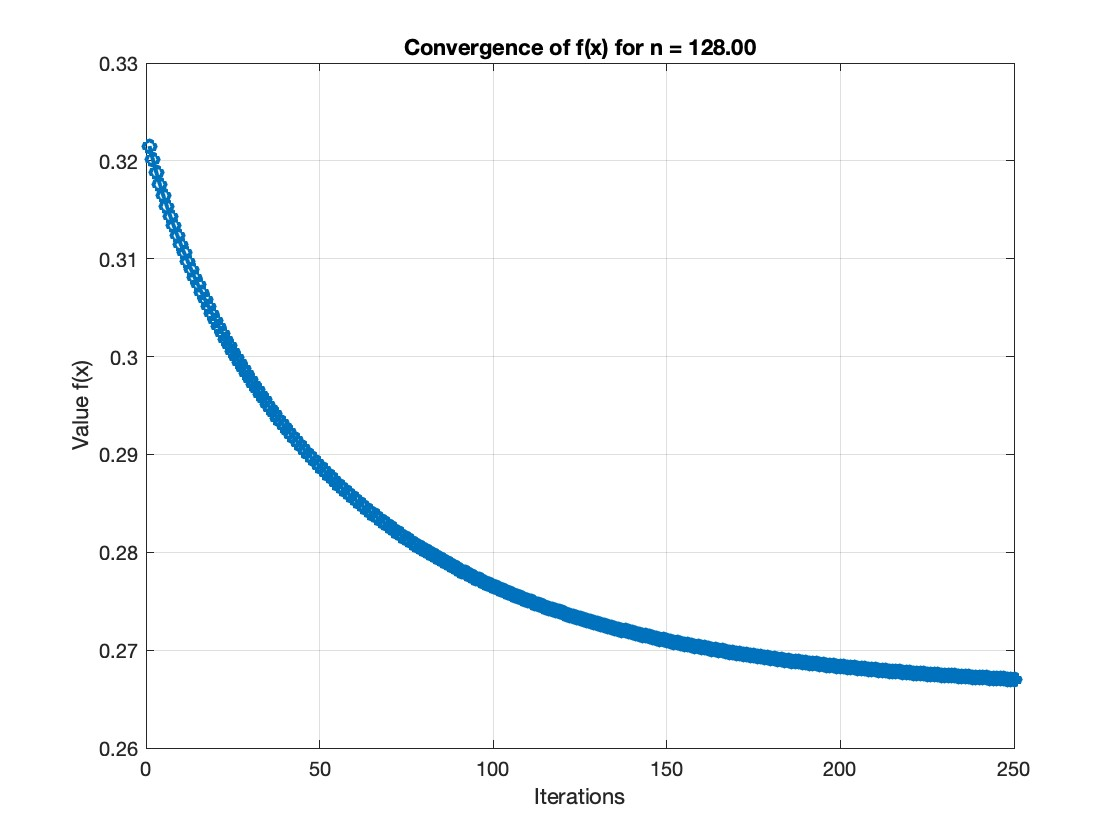
\includegraphics[width=\textwidth]{3f27.jpg}
%    \end{subfigure}
%    \begin{subfigure}[b]{0.45\textwidth}
%        \centering
%        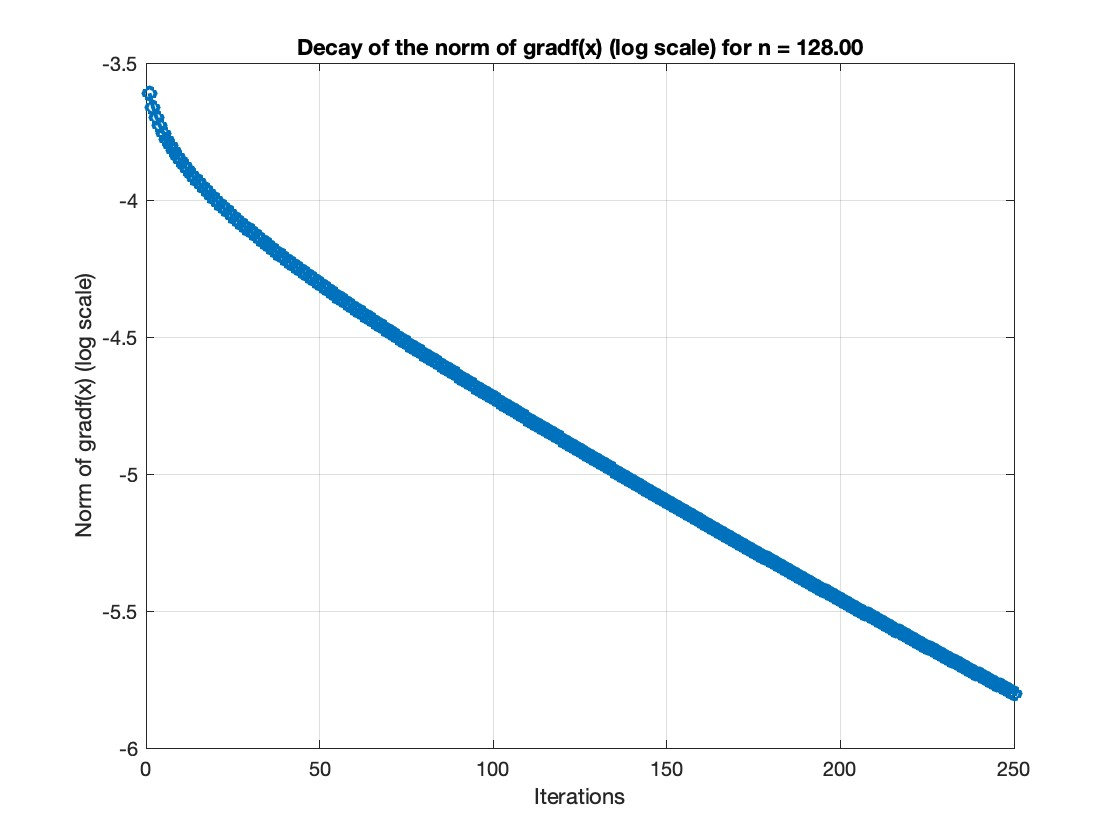
\includegraphics[width=\textwidth]{3g27.jpg}
%    \end{subfigure}
%    \caption{Experiment $27$ for $(3, 128)$}

%    \newpage

%    \begin{subfigure}[b]{0.45\textwidth}
%        \centering
%        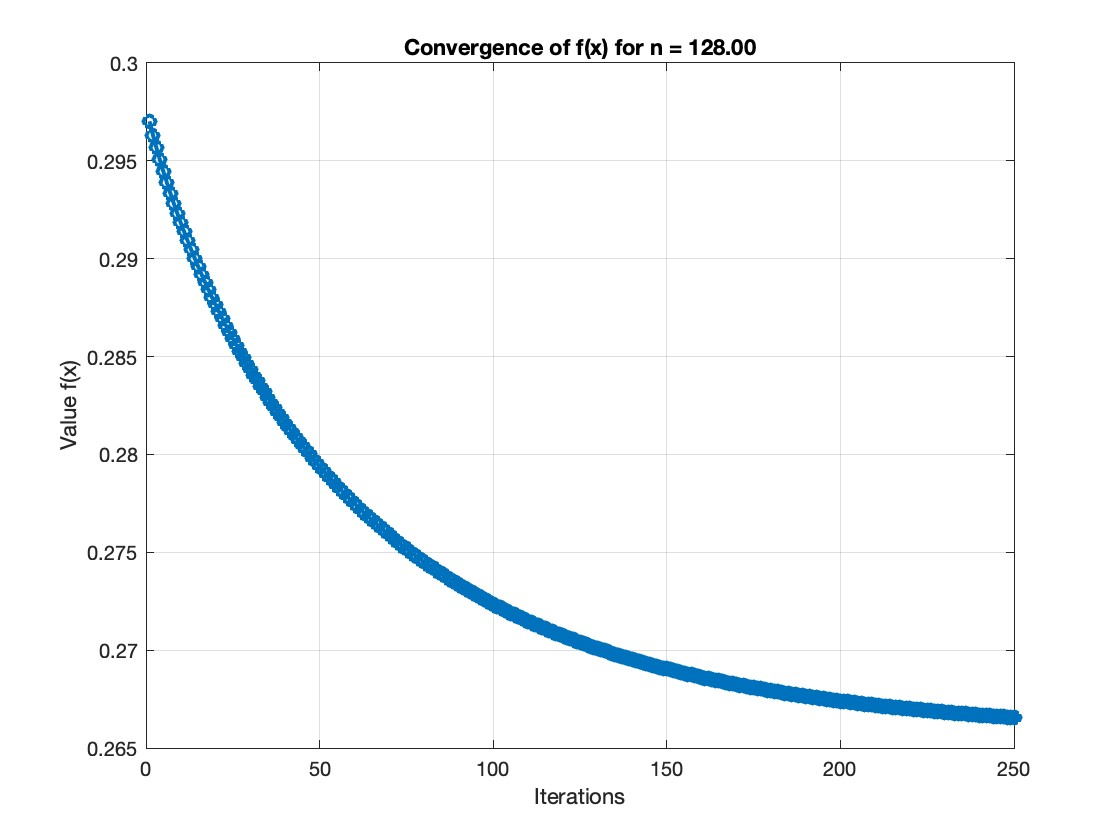
\includegraphics[width=\textwidth]{3f28.jpg}
%    \end{subfigure}
%    \begin{subfigure}[b]{0.45\textwidth}
%        \centering
%        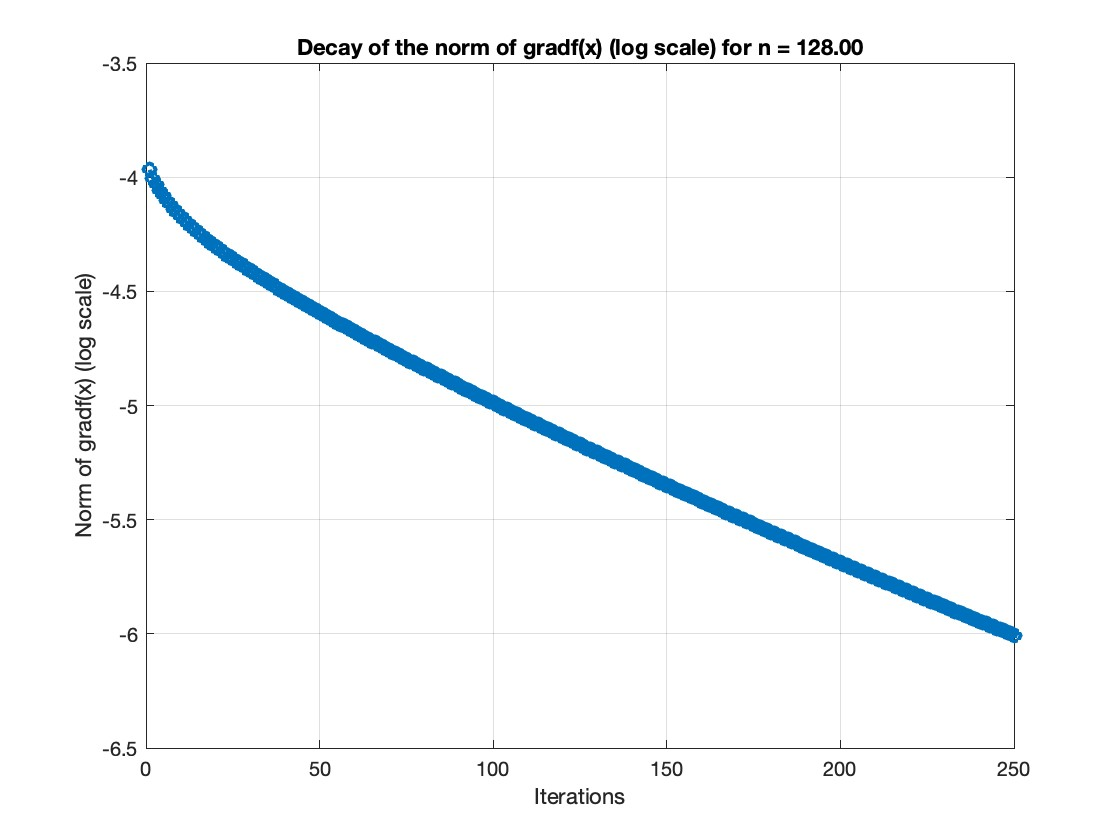
\includegraphics[width=\textwidth]{3g28.jpg}
%    \end{subfigure}
%    \caption{Experiment $28$ for $(3, 128)$}
%\end{figure}
%\begin{figure}
%    \centering
%    \begin{subfigure}[b]{0.45\textwidth}
%        \centering
%        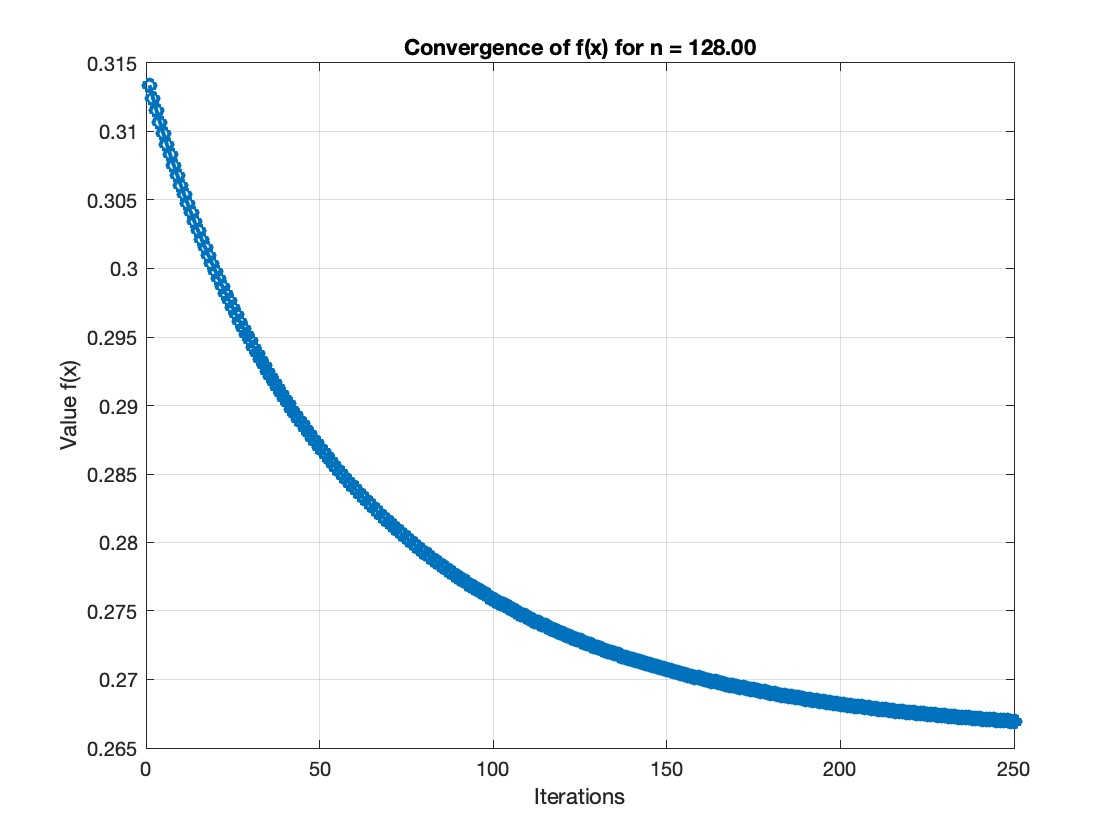
\includegraphics[width=\textwidth]{3f29.jpg}
%    \end{subfigure}
%    \begin{subfigure}[b]{0.45\textwidth}
%        \centering
%        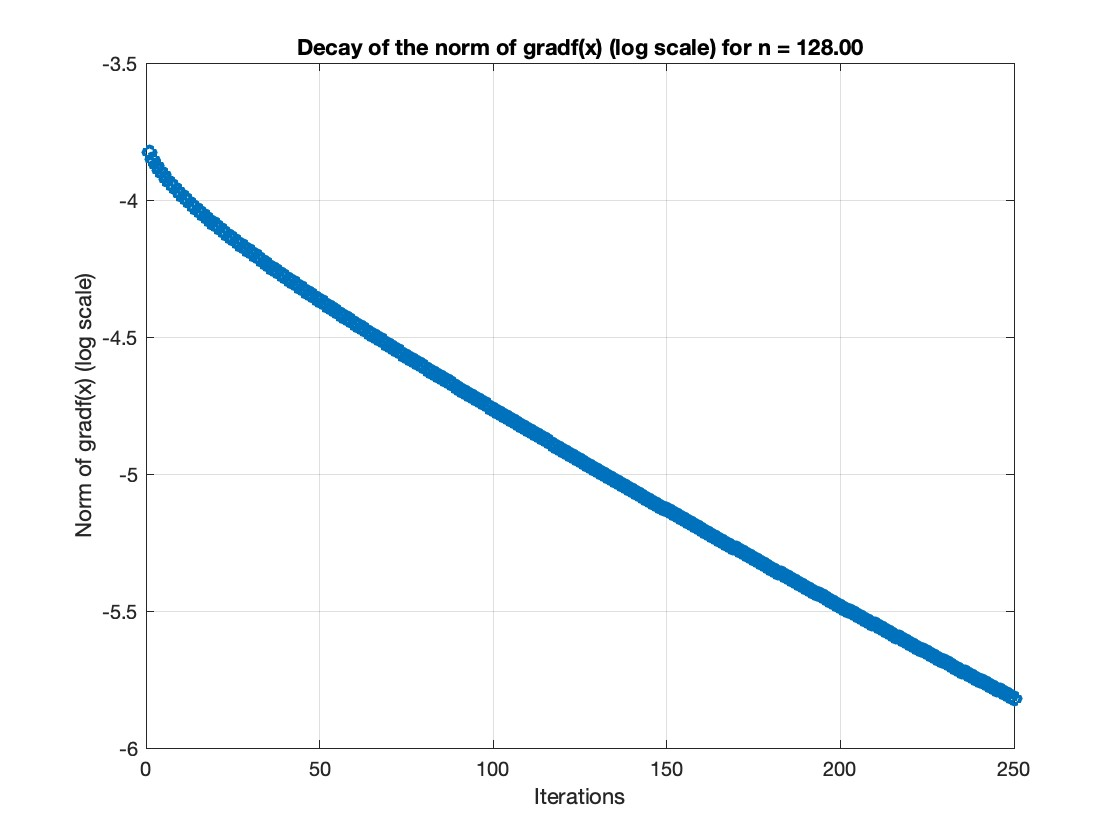
\includegraphics[width=\textwidth]{3g29.jpg}
%    \end{subfigure}
%    \caption{Experiment $29$ for $(3, 128)$}

%    \newpage

%    \begin{subfigure}[b]{0.45\textwidth}
%        \centering
%        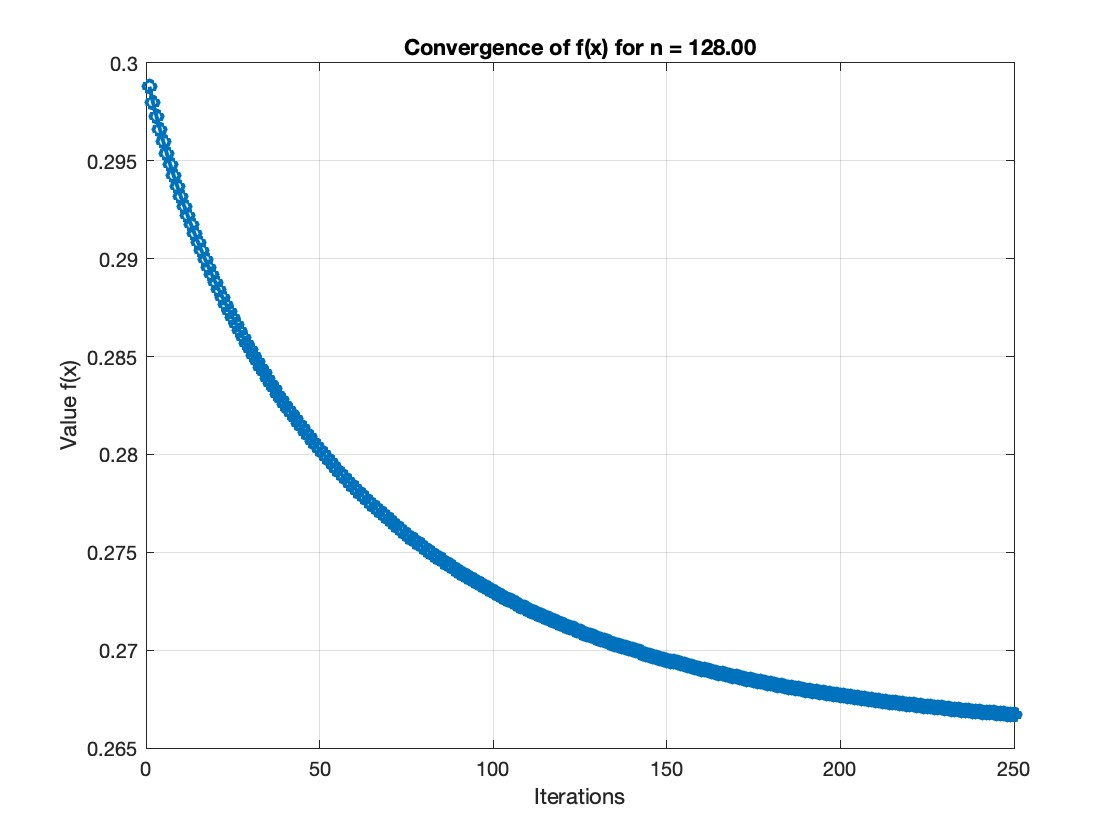
\includegraphics[width=\textwidth]{3f30.jpg}
%    \end{subfigure}
%    \begin{subfigure}[b]{0.45\textwidth}
%        \centering
%        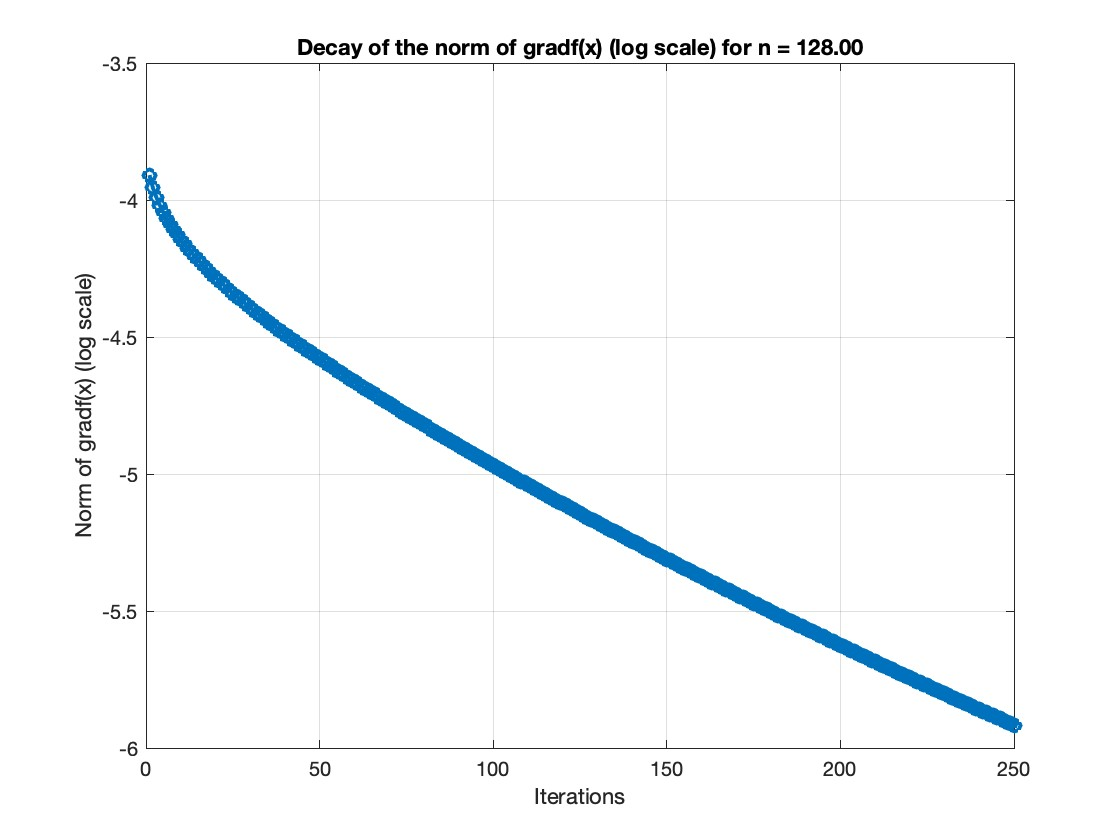
\includegraphics[width=\textwidth]{3g30.jpg}
%    \end{subfigure}
%    \caption{Experiment $30$ for $(3, 128)$}
%    \label{fig:330}
%\end{figure}
The code used to run the experiments and obtain the plots in this question is showed below. It is in the file \texttt{run\_experiments.m}. As a lot of plots are created, we suggest running this code line by line.
\begin{lstlisting}[style=Matlab-editor, numbers=left, frame=single, backgroundcolor=\color{gray!5}]
% We suggest running this code line by line, as there are a lot of plots
% being created at each line

% For reproducibility
rng(2)

% Run the experiments for d=2
[costs2_3, X2_3, ~] = Experiments(2, 3, 250, 1, true);
[costs2_4, X2_4, ~] = Experiments(2, 4, 250, 1, true);
[costs2_5, X2_5, ~] = Experiments(2, 5, 250, 1, true);
[costs2_6, X2_6, ~] = Experiments(2, 6, 250, 1, true);
[costs2_20, X2_20, ~] = Experiments(2, 20, 250, 1, true);
[costs2_100, X2_100, i2_100] = Experiments(2, 100, 250, 1, true);

% Run the experiments for d=3
[costs3_2, X3_2, ~] = Experiments(3, 2, 250, 1, true);
[costs3_3, X3_3, ~] = Experiments(3, 3, 250, 1, true);
[costs3_4, X3_4, ~] = Experiments(3, 4, 250, 1, true);
[costs3_5, X3_5, ~] = Experiments(3, 5, 250, 1, true);
[costs3_6, X3_6, ~] = Experiments(3, 6, 250, 1, true);
[costs3_12, X3_12, ~] = Experiments(3, 12, 250, 1, true);
[costs3_16, X3_16, ~] = Experiments(3, 16, 250, 1, true);
[costs3_50, X3_50, ~] = Experiments(3, 50, 250, 1, true);
[costs3_128, X3_128, i3_128] = Experiments(3, 128, 250, 1, true);

% Create table of min and max final cost function values for d=2
n = [3; 4; 5; 6; 20; 100];
Minimum = [min(costs2_3); min(costs2_4); min(costs2_5); min(costs2_6); min(costs2_20); min(costs2_100)];
Maximum = [max(costs2_3); max(costs2_4); max(costs2_5); max(costs2_6); max(costs2_20); max(costs2_100)];
Minimum = round(Minimum, 4);
Maximum = round(Maximum, 4);
table(n, Minimum, Maximum)

% Create table of min and max final cost function values for d=3
n = [2; 3; 4; 5; 6; 12; 16; 50; 128];
Minimum = [min(costs3_2); min(costs3_3); min(costs3_4); min(costs3_5); min(costs3_6); min(costs3_12); min(costs3_16); min(costs3_50); min(costs3_128)];
Maximum = [max(costs3_2); max(costs3_3); max(costs3_4); max(costs3_5); max(costs3_6); max(costs3_12); max(costs3_16); max(costs3_50); max(costs3_128)];
Minimum = round(Minimum, 4);
Maximum = round(Maximum, 4);
table(n, Minimum, Maximum)

% Visualize the best configurations for each pair
visualize(X2_3)
visualize(X2_4)
visualize(X2_5)
visualize(X2_6)
visualize(X2_20)
visualize(X2_100)
visualize(X3_2)
visualize(X3_3)
visualize(X3_4)
visualize(X3_5)
visualize(X3_6)
visualize(X3_12)
visualize(X3_16)
visualize(X3_50)
visualize(X3_128)

% Obtain the iteration number corresponding to the best configuration for
% (2, 100) and (3, 128)
i2_100
i3_128

% Visualize substantially distinct configurations obtained for n < 20
%For d = 2:
for n = [3, 4, 5, 6]
    X0 = SampleOB(2, n);
    for i = 1:15
        [X, ~, ~, ~] = RGD_BLS(X0, 1, i);
        figure;
        visualize(X)
    end
end
% For d = 3:
for n = [2, 3, 4, 5, 6, 12, 16]
    X0 = SampleOB(3, n);
    for i = [1, 2, 3, 4, 5, 10, 15, 20, 30, 40, 50, 100, 200]
        [X, ~, ~, ~] = RGD_BLS(X0, 1, i);
        figure;
        visualize(X)
    end
end
\end{lstlisting}

\subsection*{Question 13}
When running the experiments for $d=2$, we notice that the function values converge exponentially fast to the minimum. In particular they are decreasing, showing that the RGD algorithm indeed decreases the value of $f$ after each iteration. Moreover, for smaller values of $n$, the function values stabilize after very few steps. The gradient norm decreases linearly (in the log scale), except for larger values of $n$, e.g. $n=20, 100$, where it starts to decay exponentially and sometimes oscillate before following a linear decrease. Sometimes, the gradient norm oscillates within the very first iterations. This could happen because of a too high value for $\alpha$, which can cause the gradient to change too much in one iteration. This in particular depends on the initial generated point $X_0$.\\
The algorithm converged for $n\in\{3, 4, 5, 6, 20\}$ and took approximately around $30$ iterations for $n=3$, around $40$\textendash$45$ for $n=4$, around $50$\textendash$60$ for $n=5$, around $60$\textendash$70$ for $n=6$ and finally over $200$, but less than $250$ iterations, for $n=20$. For $n=100$, the algorithm did not converge after $250$ iterations. The larger $n$ is, the more iterations are needed until convergence, as we have much more points and much larger matrices.\\
Table \ref{tab:d2} shows that the minimum and maximum cost function values obtained for $n\in\{3, 4, 5, 6, 20\}$ are the same. This is a consequence of the fact that the algorithm converged for these values. For $n=100$, since there was no convergence, we observe a small difference between the minimum and maximum final cost function values, which differ by $0.0004$, an error of the order of $10^{-4}$.\\
The optimal configuration obtained for a given $n$ yields a distribution of the points on the circle forming the vertices of a regular polygon with $n$ vertices, as illustrated in Figure \ref{fig:opt2_group}: we get an equilateral triangle for $n=3$, a square for $n=4$, a pentagon for $n=5$, an hexagon for $n=6$, an icosagon for $n=20$ and finally a hectogon for $n=100$. Since $f$ is a sum of functions which are increasing on $[-1, 1)$ ($f$ is a sum of $-\log(1-x_i^Tx_j)$ for $x_i^Tx_j\in [-1, 1)$, since $X\in\text{OB}(d, n)\backslash\Delta$), the closer the points are, the smaller their scalar product $x_i^Tx_j$ is, and thus the larger those functions are. As a consequence, for larger $n$, since the points are closer to each other, the minimum value for $f$ is higher; this is indeed what we observe in Table \ref{tab:d2}, with final cost function values increasing with $n$.

\subsection*{Question 14}
For the case $d=3$, the conclusions are similar to the case $d=2$, except that for the same $n$ the algorithm needs more steps until convergence, since we are dealing with larger matrices.\\
The function values still decrease monotonically as the number of iterations increases, at an exponential rate, once again showing that the RGD algorithm correctly reduces the value of $f$ after each iteration. The norm of the gradient decays first exponentially within the very first iterations and then starts to decrease linearly (in the log scale) for small $n$. For $n\geq 4$, the norm starts to behave differently in some experiments, where it starts by decreasing exponentially, then increases a little and starts decreasing again. This can happen due to the backtracking line search algorithm changing the value of $\alpha$, which might have been too big. It can also happen if the algorithm is following the wrong direction, maybe a saddle point. Nonetheless, the function $f$ still decreases and the gradient norm ends up decreasing as well.\\
The algorithm converged for $n\in\{2, 3, 4\}$ and took approximately around $15$\textendash$20$ iterations for $n=2$, around $30$\textendash$35$ for $n=3$ and more than $80$ for $n=4$. For $n\in\{5, 6, 12, 16, 50, 128\}$, the algorithm did not converge after $250$ iterations. However, for $n<128$, the function $f$ stabilized near the minimum.\\
Table \ref{tab:d3} gives the minimum and maximum cost function values obtained for each $n$. For $n\in\{2, 3, 4\}$, the minimum and maximum values are the same, since the algorithm has converged. For the remaining values of $n$, we observe a small difference, explained by the fact that the algorithm has not converged after the $250$ iterations.\\
The optimal configurations that we obtained give points which are as far from each other as possible, except for larger $n$ where the algorithm has not converged and thus the obtained configuration is not yet optimal. In particular, for $n=2$ we get two antipodal points, for $n=3$ an equilateral triangle on an equator, for $n=4$ a regular tetrahedron, for $n=5$ two antipodal points together with an equilateral triangle on the equator, for $n=6$ a regular octahedron and for $n=12$ a regular icosahedron. These correspond precisely the the known optimal configurations, which suggests that our algorithm correctly performed the minimization of $f$. Once again, we notice that the distances between the points decrease when there are more points, yielding to an increase of the cost function values. This occurs due to the properties of $f$ discussed in the previous question.\\
\newline
We now proceed to compute the value of $f$ for the known optimal configurations for $n\in\{2, 3, 4, 5, 6, 12\}$. To this end, and since the result is unique up to rotation, we can freely choose the coordinates of the points $x_i$ as long as they give the optimal configuration. Indeed, two configurations differing only by rotation still have the same distances between the points and thus the value of $f$ at both configurations is the same.\\
\setcounter{MaxMatrixCols}{12}
\begin{itemize}
    \item For $n=2$, a matrix corresponding to the optimal configuration is given by
          $$
          X_2 = \begin{pmatrix}1 & -1\\ 0 & 0 \\ 0 & 0\end{pmatrix}.
          $$
          Using our function \texttt{Computefgradf}, we compute the value of $f$ at this point and obtain $-0.6931$.
    \item For $n=3$, a matrix giving the optimal configuration is given by
          $$
          X_3 = \begin{pmatrix}1 & -1/2 & -1/2\\ 0 & \sqrt{3}/2 & -\sqrt{3}/2\\ 0 & 0 & 0 \end{pmatrix}.
          $$
          Evaluating $f$ at this point then yields $-0.4055$.
    \item For $n=4$, a matrix for the optimal configuration is given by
          $$
          X_4 = \begin{pmatrix} 1/\sqrt{3} & 1/\sqrt{3} & -1/\sqrt{3} & -1/\sqrt{3} \\ 1/\sqrt{3} & -1/\sqrt{3} & 1/\sqrt{3} & -1/\sqrt{3} \\ 1/\sqrt{3} & -1/\sqrt{3} & -1/\sqrt{3} & 1/\sqrt{3}\end{pmatrix}.
          $$
          Evaluating $f$ at $X_4$ gives $-0.2877$.
    \item For $n=5$, a matrix giving the optimal configuration is given by
          $$
          X_5 = \begin{pmatrix} 0 & 0 & 1 & -1/2 & -1/2 \\ 0 & 0 & 0 & \sqrt{3}/2 & -\sqrt{3}/2 \\ 1 & -1 & 0 & 0 & 0\end{pmatrix}.
          $$
          Evaluating $f$ at $X_5$ gives $-0.1910$.
    \item For $n=6$, a matrix giving the optimal configuration is given by
          $$
          X_6 = \begin{pmatrix} 0 & 0 & \sqrt{2}/2 & \sqrt{2}/2 & -\sqrt{2}/2 & -\sqrt{2}/2 \\ 1 & -1 & 0 & 0 & 0 & 0 \\ 0 & 0 & \sqrt{2}/2 & -\sqrt{2}/2 & \sqrt{2}/2 & -\sqrt{2}/2 \end{pmatrix}.
          $$
          Evaluating $f$ at $X_6$ yields $-0.1386$.
    \item For $n=12$, a matrix corresponding to the optimal configuration is given by
          $$
          X_{12} = \frac{1}{\sqrt{1+\varphi^2}}
          \begin{pmatrix}
          \varphi & -\varphi & \varphi & -\varphi & 1 & -1 & 1 & -1 & 0 & 0 & 0 & 0 \\ 1 & 1 & -1 & -1 & 0 & 0 & 0 & 0 & \varphi & -\varphi & \varphi & -\varphi \\ 0 & 0 & 0 & 0 & \varphi & \varphi & -\varphi & -\varphi & 1 & 1 & -1 & -1
          \end{pmatrix}
          $$
          where $\varphi = \frac{1+\sqrt{5}}{2}$ \cite{wiki:Icosaèdre}. Evaluating $f$ at $X_{12}$ gives $0.0384$.
\end{itemize}
Altogether, Table \ref{tab:opt} shows the minima of $f$ for the optimal configurations for $n\in\{2, 3, 4, 5, 6, 12\}$. Comparing with Table \ref{tab:d3}, we notice that for $n<12$, they correspond exactly to the minimal cost function values we obtained by optimization. For $n=12$, the optimal value of $f$ is just $0.0001$ less than the minimal value we obtained. This suggests that our optimization algorithm performed correctly and converged correctly to the optimal configurations, as our visualizations in Figure \ref{fig:opt3_group} had already suggested.
\begin{table}[H]
\centering
\begin{tabular}{|c|c|c|}
\hline
$n$ & Optimal value of $f$ \\ \hline
2 & -0.6931 \\
3 & -0.4055 \\
4 & -0.2877 \\
5 & -0.1910 \\
6 & -0.1386 \\
12 & 0.0384 \\
\end{tabular}
\caption{Values of $f$ for the optimal configurations when $d=3$ and $n\in\{2, 3, 4, 5, 6, 12\}$}
\label{tab:opt}
\end{table}
The following code was used to compute the optimal configurations. It can be found in the file \texttt{opt\_conf.m}.\\
\begin{lstlisting}[style=Matlab-editor, numbers=left, frame=single, backgroundcolor=\color{gray!5}]
X_2 = [1, -1; 0, 0; 0, 0];
Computefgradf(X_2, false)

X_3 = [1, -1/2, -1/2; 0, sqrt(3)/2, -sqrt(3)/2; 0, 0, 0];
Computefgradf(X_3, false)

X_4 = [1/sqrt(3), 1/sqrt(3), -1/sqrt(3), -1/sqrt(3); 1/sqrt(3), -1/sqrt(3), 1/sqrt(3), -1/sqrt(3); 1/sqrt(3), -1/sqrt(3), -1/sqrt(3), 1/sqrt(3)];
Computefgradf(X_4, false)

X_5 = [0, 0, 1, -1/2, -1/2; 0, 0, 0, sqrt(3)/2, -sqrt(3)/2; 1, -1, 0, 0, 0];
Computefgradf(X_5, false)

X_6 = [0, 0, sqrt(2)/2, sqrt(2)/2, -sqrt(2)/2, -sqrt(2)/2; 1, -1, 0, 0, 0, 0; 0, 0, sqrt(2)/2, -sqrt(2)/2, sqrt(2)/2, -sqrt(2)/2];
Computefgradf(X_6, false)

phi = (1+sqrt(5))/2;
X_12 = [phi, -phi, phi, -phi, 1, -1, 1, -1, 0, 0, 0, 0; 1, 1, -1, -1, 0, 0, 0, 0, phi, -phi, phi, -phi; 0, 0, 0, 0, phi, phi, -phi, -phi, 1, 1, -1, -1];
X_12 = X_12 / sqrt(1+phi^2);
Computefgradf(X_12, false)
\end{lstlisting}

\newpage

\section*{Proof of optimality for $d=3$ and $n\in\{2, 3\}$}
\addcontentsline{toc}{section}{\protect\numberline{}Proof of optimality for $d=3$ and $n\in\{2, 3\}$}

\subsection*{Question 15}

The function \( f \) is a composition of smooth functions, which we will show step by step.

\begin{enumerate}
    \item The logarithm function \( \log(x) \) is smooth (i.e., \( C^\infty \)) on \( \R^+_* \). 
    
    \item The inner product \( x_i^\top x_j \) is bilinear and smooth in \( \R^d \), ensuring that \( 1 - x_i^\top x_j \) is also smooth for all \( i, j \). Since the expression \( 1 - x_i^\top x_j \) is smooth, its composition with the logarithm, \( \log(1 - x_i^\top x_j) \), remains smooth on $\R^{nd} \setminus \Delta$ (since the composition of smooth functions remains smooth).
\end{enumerate}

Thus, \( f \) is \( C^\infty \) on \( \R^{nd} \setminus \Delta \). So \( f \) is smooth on $\mathcal{M}$.

We fix \( n \in \N \),
\[
f(x_1, \ldots, x_n) = -\frac{2}{n(n-1)} \sum_{i<j} \log(1-x_i^T x_j).
\]

Let's define \( H \),
\[
H = \{x \in \R^{dn} \text{ such that there exists } i,j \text{ so that } 1-x_i^T x_j < \exp(-(n+1)n\log(2)/2)\ \text{with $x_i, x_j \in R^d$} \}
\]

\begin{align}
    h: \mathbb{R}^{dn} &\to \mathbb{R}^{\frac{n(n-1)}{2}} \\
    x &\mapsto \big(1 - x_i^\top x_j \big)_{\substack{i<j \\ i,j \in [n]}}.
\end{align}


Let \( K_k = \R \times \R \times \cdots \times ]-\infty, \exp(-(n+1)\log(2)n/2[ \times \R \times \cdots \times \R \) (where \( K_k \) is included in \( \R^{n(n+1)/2} \) and has its \( k \)-th component as the set \( ]-\infty, \exp(-(n+1)n\log(2)/2)\)[ . 

By product of open sets in \( \R^{n(n+1)/2} \), \( K_k \) is an open set, and by union of open sets, \( \bigcup K_k \) is an open set in \( \R^{n(n+1)/2} \). Since \( f \) is smooth composition of an affine function, an inner product and a linear function, thus \( f^{-1}(\bigcup K_k) = H \) is open in \( \R^d \). So \( H^c = \R^d \setminus H \) is closed.

\( Ob(d,n) \) by product of spheres (the sphere is bounded by 1 and closed since \( r^{-1}(1) = S \) where \( r \) is the inner product, which is continuous; in finite dimension this is compact) is compact.

So \( Ob(d,n) \cap H^c \) is compact (intersection of two closed sets remains closed and since the intersection is in \( Ob(d,n) \), which is bounded, it remains bounded; we are in finite dimension so we conclude that \( Ob(d,n) \cap H^c \) is compact).

For \( x \in Ob(d,n) \cap H^c \), suppose that \( x \in \Delta \). Then there exists \( i_0,j_0 \) such that \( x_{i_0} = x_{j_0} \), so \( 1-x_{i_0}^T x_{j_0} = 0 \). But since \( x \in H^c \), for every \( i,j \) (in particular for \( i_0,j_0 \)) we have  \( 0< \exp(-(n+1)n\log(2)/2) \leq 1 - x_i^T x_j \), leading to a contradiction. 

Thus, if \( x \in Ob(d,n) \cap H^c \), then \( x \notin \Delta \). Hence \( Ob(d,n) \cap H^c \subseteq M \).

We have just shown above that \( f \) is continuous on \( M \) so \( f \) is continuous on \( Ob(d,n) \cap H^c \). Moreover, \( Ob(d,n) \cap H^c \) is compact. Hence, according to Weierstrass Theorem, \( f \) is bounded and attains its bounds on this compact, with minimizers that we denote by \( x^* \).

Take \( x_1 \in S(\R^d) \), \( x_2 = -x_1 \), and \( x_i = 0 \) for \( i > 2 \). Let \( x' = (x_1, \ldots, x_n) \). Then \( x' \) is in \( Ob(d,n) \cap H^c \) by construction, and
\[
f(x') = -\log(2) \cdot \frac{2}{n(n-1)}.
\]

For \( x \in Ob(d,n) \setminus (Ob(d,n) \cap H^c) \), let \( i_0,j_0 \) be the coordinates where the condition fails. Then (first inequality is given by the definition of H):
\[
\frac{n(n-1)}{2}f(x) = -\log(1-x_{i_0}^T x_{j_0}) + \sum_{\substack{i<j \\ (i,j)\neq(i_0,j_0)}} -\log(1-x_i^T x_j) \geq -\frac{n(n+1)\log(2)}{2} -\sum_{i<j} \log(1-x_i^T x_j) \geq -\frac{n(n+1)\log(2)}{2} + \frac{n(n+1)}{2} = 0
\]


Justification of the second inequality:

By the Cauchy-Schwarz inequality, we have  
\[
x_i^\top x_j \leq \|x_i\| \|x_j\| = 1.
\]
Thus,  
\[
0 < 1 - x_i^\top x_j < 2.
\]
Since the function \( t \mapsto -\log(t) \) is decreasing, it follows that  
\[
-\log(2) < -\log(1 - x_i^\top x_j).
\]

Thus \( f(x) \geq 0 > f(x') \geq f(x^*) \)  (1)

Therefore, for any \( x \in Ob(d,n) \):
\begin{itemize}
    \item If \( x \in Ob(d,n) \cap H^c \), by definition of minimizer on \( Ob(d,n) \cap H^c \), \( f(x) \geq f(x^*) \).
    \item If \( x \in Ob(d,n) \setminus (Ob(d,n) \cap H^c) \), we just showed \( f(x) > f(x^*) \) in (1).
\end{itemize}



Thus for every \( x \in Ob(d,n) \), \( f(x) \geq f(x^*) \), so \( x^* \) is a minimizer on \( Ob(d,n) \). So f has a minimizer on \( Ob(d,n) \).



If \( x \) is a minimizer and \( x \in Ob(d,n) \setminus (Ob(d,n) \cap H^c) \), (1) shows \( f(x) > f(x') \), which contradicts the definition of a minimizer. So \( x \) cannot be a minimizer on \( Ob(d,n) \). Thus, we have showed that minimizers are  not in \(Ob(d,n) \setminus (Ob(d,n) \cap H^c) \) so in \( Ob(d,n) \cap H^c \).

And \( (Ob(d,n) \cap H^c) \subseteq M \). So minimizers of \( f \) are in \( M \).


\subsection*{Question 16}
Define the set:
\begin{equation}
    H = \{ x = (x_1, -x_1) \mid x_1 \in \mathbb{R}^d \}.
\end{equation}

We will prove that H is the set of minimizer of f.


For \( n = 2 \), the cost function simplifies to:  
\[
f(x_1, x_2) = -\frac{2}{2(2-1)} \log(1 - x_1^\top x_2) = -\log(1 - x_1^\top x_2).
\]



According to Question 15, the function $f$ has a minimum at $x^* = (x_1^*, x_2^*)$ on $\mathcal{M}$. 

The function $h(t) = -\log(1 - t)$ is decreasing on $\mathbb{R}$, so $h$ is minimized when $t$ is minimized. Thus, minimizing $f$ is equivalent to minimizing $x_1^\top x_2$, meaning $x^*$ minimizes $h(x) = x_1^\top x_2$.

On the one hand, by the Cauchy-Schwarz inequality, we have:
\begin{equation}
    |x_1^\top x_2| \leq (\|x_1\| \|x_2\|)^{\frac{1}{2}} = 1.
\end{equation}
Equality holds if and only if $x_1 = \alpha x_2$ for some $\alpha \in \mathbb{R}$. Since $x_1$ and $x_2$ lie on the unit sphere, we obtain:
\begin{equation}
    1 = \|x_1\|^2 = \|\alpha x_2\|^2 = \alpha^2 \|x_2\|^2 = \alpha^2,
\end{equation}
which implies $\alpha \in \{-1,1\}$.

Since $h(x^*) \leq h(y)$ for every $y \in \mathcal{M}$, consider $y = (x_1^*, -x_1^*)$, yielding:
\begin{equation}
    h(x^*) \leq -1.
\end{equation}
However, the Cauchy-Schwarz inequality states that $h(y) \geq -1$ for all $y \in \mathcal{M}$, and in particular for $y = x^*$. Thus, we conclude:
\begin{equation}
    h(x^*) = -1.
\end{equation}
By the equality condition of Cauchy-Schwarz, we obtain $x_1^* = x_2^*$ or $x_1^* = -x_2^*$. The first case leads to $h(x^*) = 1$, contradicting our inequality, so we must have $x_1^* = -x_2^*$. 
Hence, x* $\in$ H. 


Conversely, consider any $x \in H$:
\begin{equation}
    f(x) = -\log(1 - (-1)) = -\log(2).
\end{equation}
Thus, $f$ is constant over $H$, and in particular (since $x^*$ in H as proved above), $f(x) = f(x^*) \leq f(y)$ for every $y \in \mathcal{M}$. Hence, by definition x i also a minimizer of f on $\mathcal{M}$.


Hence, $x$ is a minimizer of $f$ in $OB(d,n)$ if and only if $x = (x_1, -x_1)$ for some $x_1 \in S^{d-1}$ which proves the result found in question 14. 

For \( n = 3 \), see below Question 19.

\subsection*{Question 17}  
    Since we have  
\[
\operatorname{grad} f(X) = \frac{1}{n(n-1)}  
\left[  
(I - x_1 x_1^T) \sum_{j \neq 1} \frac{1}{1 - x_1^T x_j} x_j,  
\ldots,  
(I - x_n x_n^T) \sum_{j \neq n} \frac{1}{1 - x_n^T x_j} x_j  
\right].
\]  

Setting \( \operatorname{grad} f(X) = 0 \), we obtain  
\[
\forall i \in \{1, \dots, n\}, \quad  (I - x_i x_i^T) \sum_{j \neq i} \frac{x_j}{1 - x_i^T x_j} = 0,  
\]
since \( x_i, x_j \notin \Delta \).

Moreover, using the identity
\[
\langle x_i, x_j \rangle = \frac{1}{2} (||x_i||^2 + ||x_j||^2 - ||x_i - x_j||^2),
\]
we obtain
\[
1 - x_i^T x_j = \frac{||x_i - x_j||^2}{2}.
\]
Thus,
\[
h(x_i, x_j) = \log (1 - x_i^T x_j) = \log(||x_i - x_j||^2) - \log(2).
\]
Differentiating, we get
\[
\nabla h(x_i, x_j) = \frac{x_i - x_j}{||x_i - x_j||^2}.
\]
Applying this to our gradient equation,
\[
\forall i \in \{1, \dots, n\}, \quad (I - x_i x_i^T) \sum_{j \neq i} \frac{x_i - x_j}{||x_i - x_j||^2} = 0.
\]
Expanding the term,
\[
x_i x_i^T \frac{x_i - x_j}{||x_i - x_j||^2} = \frac{x_i x_i^T x_i - x_i x_i^T x_j}{||x_i - x_j||^2} = \frac{x_i (1 - x_i^T x_j)}{||x_i - x_j||^2} = \frac{x_i \cdot (||x_i - x_j||^2 / 2)}{||x_i - x_j||^2} = \frac{x_i}{2}.
\]
Thus, we finally obtain
\[
\forall i \in \{1, \dots, n\}, \quad \sum_{j \neq i} \frac{x_i - x_j}{||x_i - x_j||^2} - \sum_{j \neq i} \frac{x_i}{2} = 0.
\]
Simplifying,
\[
\forall i \in \{1, \dots, n\}, \quad \sum_{j \neq i} \frac{x_i - x_j}{||x_i - x_j||^2} - \frac{(N-1) x_i}{2} = 0.
\]
Rearranging, we conclude:
\[
\sum_{j \neq i} \frac{x_i - x_j}{||x_i - x_j||^2} = \frac{(N-1) x_i}{2}.
\]


\subsection*{Question 18}

Since we sum the previous equality over \( i \), we obtain:
\[
\sum_{i=1}^{N}  \sum_{j \neq i} \frac{x_i - x_j}{||x_i - x_j||^2} = \sum_{i=1}^{N}\frac{(N-1) x_i}{2}.
\]
Rewriting the summation,
\[
\sum_{i =1}^{N} \sum_{j<i} \frac{x_i - x_j}{||x_i - x_j||^2} + \sum_{i=1}^{N} \sum_{j>i} \frac{x_i - x_j}{||x_i - x_j||^2} =\sum_{i =1}^{N} \sum_{j<i} \frac{x_i - x_j}{||x_i - x_j||^2} - \sum_{i =1}^{N} \sum_{j<i} \frac{x_i - x_j}{||x_i - x_j||^2} = \sum_{i=1}^{N}\frac{(N-1) x_i}{2}.
\]
Hence,
\[
\sum_{i=1}^{N}\frac{(N-1) x_i}{2} = 0.
\]
Thus, we obtain the result:
\[
\sum_{i=1}^{N} x_i = 0.
\]




\subsection*{Question 19}

On the one hand, according to question 17, we have:
\[
||x - x_j||^2 = 2 (1 - \langle x, x_j \rangle).
\]
Furthermore, using the result from question 18:
\[
\sum_{j=1}^{N} \langle x, x_j \rangle = \langle x, \sum_{j=1}^{N} x_j \rangle = 0, \quad \text{since } \sum_{j=1}^{N} x_j = 0.
\]
Thus, we obtain:
\[
\sum_{j=1}^{N} ||x - x_j||^2 = \sum_{j=1}^{N} 2 = 2N.
\]


\subsection*{Question 16}
Let's prove the case $n=3$. According to Question 15, the function $f$ has a minimizer $x^*$ on $\mathcal{M}$, and from the course, we know that $x^* = (x_1, x_2, x_3)$ is a critical point. 

From Question 18, we have the constraint:
\begin{equation}
    x_1 + x_2 + x_3 = 0.
\end{equation}
For any indices $i, j, k \in \{1,2,3\}$, we also know that:
\begin{equation}
    \| -x_i - x_j \|^2 = \| x_k \|^2 = 1.
\end{equation}
Expanding the norm squared:
\begin{align*}
    \| x_i + x_j \|^2 &= \| x_i \|^2 + \| x_j \|^2 + 2 \langle x_i, x_j \rangle \\
    &= 2 + 2 \langle x_i, x_j \rangle.
\end{align*}
Hence
\begin{equation}
    2\langle x_i, x_j \rangle = 1-2 \implies \langle x_i, x_j \rangle=-\frac{1}{2}
\end{equation}

Thus, the minimizer is a point on the equilateral triangle inscribed on the sphere.

Define the set:
\begin{equation}
    H = \left\{ x = (x_1, x_2, x_3) \in \mathbb{R}^{3d} \mid \langle x_i, x_j \rangle = -\frac{1}{2}, \quad \forall i \neq j \right\}.
\end{equation}
We have proven that if $x^*$ is a minimizer of $f$, then $x^* \in H$. Now, we show that any element of $H$ is a minimizer of $f$ (using the fact that $x^*$ exists according to question 15 and its minimal property).

Let $x \in H$, then:
\begin{align*}
    f(x) &= -\frac{1}{3} \left( \log(1 - (-1/2)) + \log(1 - (-1/2)) + \log(1 - (-1/2)) \right) \\
         &= -\frac{1}{3} \left( 3 \log(3/2) \right) \\
         &= \log(2/3).
\end{align*}
Thus, $f$ is constant on $H$, meaning that:
\begin{equation}
    f(x) = f(x^*) \leq f(y), \quad \forall y \in \mathcal{M}.
\end{equation}
By the definition of a minimum, $x$ is a minimizer of $f$ on $\mathcal{M}$.

We have shown that $x$ is a minimizer of $f$ if and only if $x \in H$. This proves that the minimizers in the case $n=3$ are the points forming an equilateral triangle on the sphere or in other words satisfying:
\begin{equation}
    \langle x_i, x_j \rangle = \cos(120^\circ) = -\frac{1}{2}.
\end{equation}







\subsection*{Question 20}


Let $\mathcal{H}$ denote the set of critical points of $f$, x $\in \mathcal{M}$. From the condition $\sum_{i=1}^n x_i = 0$ and the other critical point conditions, we deduce that $\langle x_i, x_j \rangle = c$ for some constant $c$. Consequently, since $f$ depends only on the pairwise inner products $\langle x_i, x_j \rangle$ then $f$ is therefore constant over $\mathcal{H}$. 

This implies that the set of critical points of $f$ coincides with its set of global minima (by the same reasoning as in Question~16). Hence, all critical points are minima, and Riemannian gradient descent converges to a global minimum of $f$.

Furthermore, $f$ satisfies the \textit{sufficient decrease property} locally (by Taylor expansion arguments), which guarantees that Riemannian gradient descent with an adaptive step size converges to a critical point. 



\newpage

\section*{Using Manopt}
\addcontentsline{toc}{section}{\protect\numberline{}Using Manopt}

\subsection*{Question 21}
We implemented the same optimization algorithm using PyManopt. We defined the manifold as follows. 

\begin{lstlisting}[style=Python-editor]
d = 2  # Dimension of each column vector
n = 3  # Number of columns in matrix X

manifold = Oblique(d, n)

\end{lstlisting}
We defined the same cost function as before.
\begin{lstlisting}[style=Python-editor]
@pymanopt.function.numpy(manifold)
def cost(X):
    d, n = X.shape
    M = X.T @ X  # Compute the Gram matrix (n, n)
    i_idx, j_idx = np.triu_indices(n, k=1)  # Get indices where i < j
    sum_log = np.sum(np.log(1 - M[i_idx, j_idx]))
    return -2 * sum_log / (n * (n - 1))

manifold = Oblique(d, n)

\end{lstlisting}

When performing optimization with Pymanopt, you can either analytically compute the Riemannian gradient and pass it as input to the "Problem", or provide the Euclidean gradient and let Pymanopt automatically project it onto the tangent space. Below, both approaches are implemented.
\subsubsection*{Automatic Projection of Euclidean Gradient}
\begin{lstlisting}[style=Python-editor]
@pymanopt.function.numpy(manifold)
def grad(X):
    d, n = X.shape
    gradX = np.zeros_like(X)
    M = X.T @ X  # Compute Gram matrix
    for i in range(n):
        v = np.zeros(d)
        for j in range(n):
            if i != j:
                v += X[:, j] / (1 - M[i, j])
        gradX[:, i] = v
    return 2 * gradX / (n * (n - 1))
    problem = Problem(manifold=manifold, cost=cost, euclidean_gradient=grad)
    check_gradient(problem)  #Verify gradient correctness

    optimizer = optimizers.SteepestDescent(log_verbosity=2)
    result = optimizer.run(problem)
\end{lstlisting}

\begin{figure}[H]
    \centering
    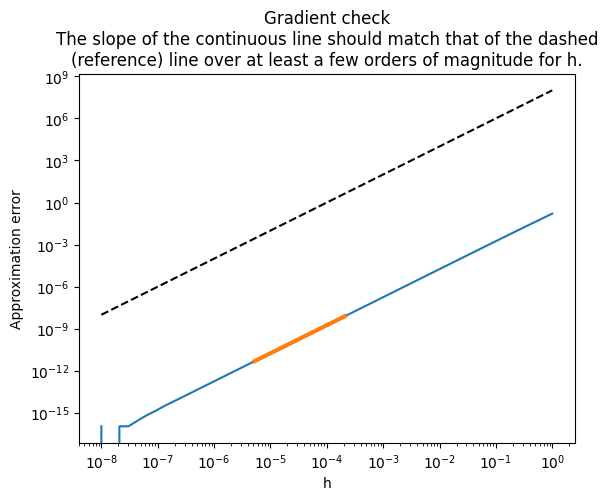
\includegraphics[width=0.8\textwidth]{euc_gradcheck21.png}
    \caption{The comparison of the numerical gradient and the projection of analytical gradient}
    \label{fig:example}
\end{figure}

\begin{figure}[H]
    \centering
    \includegraphics[width=0.8\textwidth]{euc_gradconv21.png}
    \caption{Convergence of gradient norm and cost value}
    \label{fig:example}
\end{figure}
\begin{figure}[H]
    \centering
    \includegraphics[width=0.8\textwidth]{euc_pint21.png}
    \caption{Configuration of optimal point}
    \label{fig:example}
\end{figure}
\subsubsection*{Analytical Riemannian Gradient}
\begin{lstlisting}[style=Python-editor]
@pymanopt.function.numpy(manifold)
def rie_grad(X):
    d, n = X.shape
    gradX = np.zeros_like(X)
    M = X.T @ X  
    for i in range(n):
        v = np.zeros(d)
        for j in range(n):
            if i != j:
                v += X[:, j] / (1 - M[i, j])
        gradX[:, i] = v - X[:, i] * (X[:, i].dot(v)) 
    return 2*gradX / (n * (n - 1))
    problem = Problem(manifold=manifold, cost=cost, riemannian_gradient=rie_grad)
    check_gradient(problem)  # Verify gradient correctness

    optimizer = optimizers.SteepestDescent(log_verbosity=2)
    result = optimizer.run(problem)

\end{lstlisting}
\begin{figure}[H]
    \centering
    \includegraphics[width=0.8\textwidth]{rie_gradcheck21.png}
    \caption{The comparison of the numerical gradient and the projection of analytical gradient}
    \label{fig:example}
\end{figure}
\begin{figure}[H]
    \centering
    \includegraphics[width=0.8\textwidth]{rie_gradconv21.png}
    \caption{Convergence of gradient norm and cost value}
    \label{fig:example}
\end{figure}
\begin{figure}[H]
    \centering
    \includegraphics[width=0.8\textwidth]{rie_point21.png}
    \caption{Configuration of optimal point}
    \label{fig:example}
\end{figure}
The value of the cost function after optimization is $-4.0546$ for both methods, which is generally consistent with the result from the previous question.
\subsection*{Question 22}
The same optimization was conducted using the Automatic Projection of the Euclidean Gradient with parameters $d=3$ and $n=128$.
\begin{lstlisting}[style=Python-editor]
d = 3     
n = 128     
manifold_2 = Oblique(d, n)
@pymanopt.function.numpy(manifold_2)
def cost(X):
    d, n = X.shape
    M = X.T @ X  
    i_idx, j_idx = np.triu_indices(n, k=1)
    sum_log = np.sum(np.log(1 - M[i_idx, j_idx]))
    return -2*sum_log / (n * (n - 1))

@pymanopt.function.numpy(manifold_2)
def grad(X):
    d, n = X.shape
    gradX = np.zeros_like(X)
    M = X.T @ X  
    for i in range(n):
        v = np.zeros(d)
        for j in range(n):
            if i != j:
                v += X[:, j] / (1 - M[i, j])
        gradX[:, i] = v 
    return 2*gradX / (n * (n - 1))

problem = Problem(manifold=manifold_2, cost=cost, euclidean_gradient=grad)
check_gradient(problem)
optimizer = optimizers.SteepestDescent(log_verbosity=2)
result = optimizer.run(problem)

\end{lstlisting}
\begin{figure}[H]
    \centering
    \includegraphics[width=0.8\textwidth]{gradcheck22.png}
    \caption{The comparison of the numerical gradient and the projection of analytical gradient}
    \label{fig:example}
\end{figure}
\begin{figure}[H]
    \centering
    \includegraphics[width=0.8\textwidth]{gradconv22.png}
    \caption{Convergence of gradient norm and cost value}
    \label{fig:example}
\end{figure}
\begin{figure}[H]
    \centering
    \includegraphics[width=0.8\textwidth]{point22.png}
    \caption{Configuration of optimal point}
    \label{fig:example}
\end{figure}
\subsection*{Question 23}
The same optimization problem was solved using the conjugate gradient method.
\begin{lstlisting}[style=Python-editor]
optimizer = optimizers.ConjugateGradient(log_verbosity=2)
result = optimizer.run(problem)

\end{lstlisting}
\begin{figure}[H]
    \centering
    \includegraphics[width=0.8\textwidth]{gradconv23.png}
    \caption{Convergence of gradient and cost value}
    \label{fig:example}
\end{figure}
\begin{figure}[H]
    \centering
    \includegraphics[width=0.8\textwidth]{point23.png}
    \caption{Configuration of optimal point}
    \label{fig:example}
\end{figure}
In Steepest Gradient Descent, the algorithm did not satisfy the convergence condition (gradient norm smaller than $ 10^{-7}$) within the maximum number of iterations (1000). However, in Conjugate Gradient Descent, convergence was achieved in 190 iterations. This indicates that Conjugate Gradient Descent converged faster than Steepest Descent.
\newpage
\section*{Dealing with $\Delta$}
\addcontentsline{toc}{section}{\protect\numberline{}Dealing with $\Delta$}

\subsection*{Question 24}
We are going to construct an example of an initial matrix $X_0 \in\text{OB}(d, n)\backslash\Delta$ and a step size $\alpha$ such that after one step of Riemannian gradient descent $X_0$ is mapped to a point in $\Delta$. We are going to construct such an example for the case $d=2$ and $n=4$, where the optimal configuration is a square on the unit circle. Let $X_0$ be defined by
$$
X_0 = 
\begin{pmatrix}
    -\sqrt{2}/2 & -\sqrt{2}/2 & 1/2 & 1/2 \\
    \sqrt{2}/2 & -\sqrt{2}/2 & \sqrt{3}/2 & -\sqrt{3}/2
\end{pmatrix}.
$$
We can visualize $X_0$ in Figure \ref{fig:q24x0}. Writing $X_0 = [x_1\text{ }x_2\text{ }x_3\text{ }x_4]$, then $x_1$ and $x_2$ are the two points on the left and points $x_3$ and $x_4$ are the two points on the right.
\begin{figure}[H]
    \centering
    \includegraphics[width=8cm]{q24x0.jpg}
    \caption{Visualization of the initial point $X_0$}
    \label{fig:q24x0}
\end{figure}
The idea is the following. After the first iteration in the Riemannian gradient descent, points $x_1$ and $x_2$ won't move a lot, whereas points $x_3$ and $x_4$ will move to the right, in order to maximize their distance with $x_1$ and $x_2$. We then aim at choosing an $\alpha$ such that the intensity by which we move along the opposite of the direction of the gradient of $f$ at $X$ for the coordinates $x_3$ and $x_4$ will move both $x_3$ and $x_4$ to the same point, namely the point with coordinates $(1, 0)$. In this case, the resulting matrix will be in $\Delta$ since its last two columns will be the same. With our choice of retraction, the way to move on the circle along a given direction is to follow the tangent direction and then to project the result orthogonally into the circle. Figure \ref{fig:q24tan} illustrates our aim.
\begin{figure}[H]
    \centering
    \includegraphics[width=10cm]{q24tan.png}
    \caption{Illustration of the desired position (red point) for $x_3$ and $x_4$ after the first step of RGD}
    \label{fig:q24tan}
\end{figure}
After one step of RGD, points $x_3$ and $x_4$ are going to move in the direction of the tangent lines, showed in Figure \ref{fig:q24tan}, towards the right. If we move along those directions until intersecting the $x$-axis, the orthogonal projection will give point $(1, 0)$. Since $x_3$ and $x_4$ are symmetric with respect to the $x$-axis, there must be an $\alpha$ leading both points to $(1, 0)$. Such an alpha must satisfy
\begin{align*}
    & (x_3 - \alpha \cdot\text{grad}f(X_0)_{23})_2 = 0\\
    & (x_4 - \alpha\cdot\text{grad}f(X_0)_{24})_2 = 0
\end{align*}
where $\text{grad}f(X_0)_{ij}$ denotes the element in the $i^{\text{th}}$ row and $j^{\text{th}}$ column of $\text{grad}f(X_0)$ and the subscript $2$ means we look at the second coordinate of the vector. In particular, by symmetry of our initial configuration, the two expressions are equal up to sign flip (since the second coordinate of $x_3$ is minus the second coordinate of $x_4$ and the gradient at $x_3$ has a slope equal to minus the slope of the gradient at $x_4$). Hence, an expression for $\alpha$ is given by
$$
\alpha = \frac{(x_3)_2}{\text{grad}f(X_0)_{23}}.
$$
The code below, which can be found in the file \texttt{counter\_example.m}, creates the matrix $X_0$ and computes the gradient of $f$ at $X_0$ and the value of $\alpha$ given by the expression above. It then computes the retraction
$$
R_{X_0}(-\alpha\cdot \text{grad}f(X_0))
$$
as is done in the first step of the Riemannian gradient descent. The output is the matrix
$$
R_{X_0}(-\alpha\cdot \text{grad}f(X_0)) =
\begin{pmatrix}
    -0.8997 & -0.8997 & 1 & 1 \\
    0.4366 & -0.4366 & 0 & 0
\end{pmatrix}
$$
which indeed belongs to $\Delta$, as the last two columns are identical.\\
Applying then RGD with $1$ iteration returns the matrix above and a function value of infinity. This is not surprising as, since the matrix is in $\Delta$, the logarithm is equal to zero for $i=3, j=4$ and thus goes to $-\infty$, which implies that $f$ goes to $+\infty$. Applying RGD with $2$ iterations then gives NaN for the last two columns of the matrix and also for the function value.\\
\begin{lstlisting}[style=Matlab-editor, numbers=left, frame=single, backgroundcolor=\color{gray!5}]
% Example where X_0 is mapped to Delta after one step of RGD

% Initial matrix
X_0 = [-sqrt(2)/2, -sqrt(2)/2, 1/2, 1/2; sqrt(2)/2, -sqrt(2)/2, sqrt(3)/2, -sqrt(3)/2];

% Gradient
[~, gradf] = Computefgradf(X_0, true);

% Value for alpha
alpha = sqrt(3) / (2 * gradf(2, 3));

% Retraction
Retraction(X_0, -alpha*gradf)

% Apply RGD with 1 and then 2 iterations to see what happens
RGD_BLS(X_0, alpha, 1)
RGD_BLS(X_0, alpha, 2)
\end{lstlisting}

\newpage


\clearpage
\bibliographystyle{plain}
\bibliography{biblio}


\end{document}